% -*- Mode:TeX -*-


% IMPORTANT: The official thesis specifications are available at:
%
%            http://libraries.mit.edu/archives/thesis-specs/


% **************************************************************************************************************
% A Classic Thesis Style
% An Homage to The Elements of Typographic Style
%
% Copyright (C) 2015 André Miede http://www.miede.de
%
% If you like the style then I would appreciate a postcard. My address 
% can be found in the file ClassicThesis.pdf. A collection of the 
% postcards I received so far is available online at 
% http://postcards.miede.de
%
% License:
% This program is free software; you can redistribute it and/or modify
% it under the terms of the GNU General Public License as published by
% the Free Software Foundation; either version 2 of the License, or
% (at your option) any later version.
%
% This program is distributed in the hope that it will be useful,
% but WITHOUT ANY WARRANTY; without even the implied warranty of
% MERCHANTABILITY or FITNESS FOR A PARTICULAR PURPOSE.  See the
% GNU General Public License for more details.
%
% You should have received a copy of the GNU General Public License
% along with this program; see the file COPYING.  If not, write to
% the Free Software Foundation, Inc., 59 Temple Place - Suite 330,
% Boston, MA 02111-1307, USA.
%
% **************************************************************************************************************
\RequirePackage{fix-cm} % fix some latex issues see: http://texdoc.net/texmf-dist/doc/latex/base/fixltx2e.pdf
\documentclass[ twoside,openright,titlepage,numbers=noenddot,headinclude,%1headlines,% letterpaper a4paper
                footinclude=true,cleardoublepage=empty,abstractoff, % <--- obsolete, remove (todo)
                BCOR=5mm,paper=letter,fontsize=11pt,%
                ngerman,american,%
                ]{scrreprt}


% ***************************************
% Note: Make all your adjustments in here
% ***************************************
% \pdfminorversion=4  % For compatibility w/ Miklos' Acrobat installation...
% ****************************************************************************************************
% classicthesis-config.tex
% formerly known as loadpackages.sty, classicthesis-ldpkg.sty, and classicthesis-preamble.sty
% Use it at the beginning of your ClassicThesis.tex, or as a LaTeX Preamble
% in your ClassicThesis.{tex,lyx} with % ****************************************************************************************************
% classicthesis-config.tex
% formerly known as loadpackages.sty, classicthesis-ldpkg.sty, and classicthesis-preamble.sty
% Use it at the beginning of your ClassicThesis.tex, or as a LaTeX Preamble
% in your ClassicThesis.{tex,lyx} with % ****************************************************************************************************
% classicthesis-config.tex
% formerly known as loadpackages.sty, classicthesis-ldpkg.sty, and classicthesis-preamble.sty
% Use it at the beginning of your ClassicThesis.tex, or as a LaTeX Preamble
% in your ClassicThesis.{tex,lyx} with \input{classicthesis-config}
% ****************************************************************************************************
% If you like the classicthesis, then I would appreciate a postcard.
% My address can be found in the file ClassicThesis.pdf. A collection
% of the postcards I received so far is available online at
% http://postcards.miede.de
% ****************************************************************************************************

% ****************************************************************************************************
% 1. Configure classicthesis for your needs here, e.g., remove "drafting" below
% in order to deactivate the time-stamp on the pages
% ****************************************************************************************************
%\PassOptionsToPackage{eulerchapternumbers,%drafting,%
%				 pdfspacing,%floatperchapter,%linedheaders,%
%				 subfig,beramono,eulermath}{classicthesis}		

\PassOptionsToPackage{eulerchapternumbers,drafting,%
				 pdfspacing,%floatperchapter,%linedheaders,%
				 subfig,eulermath}{classicthesis}									
% ********************************************************************
% Available options for classicthesis.sty
% (see ClassicThesis.pdf for more information):
% drafting
% parts nochapters linedheaders
% eulerchapternumbers beramono eulermath pdfspacing minionprospacing
% tocaligned dottedtoc manychapters
% listings floatperchapter subfig
% ********************************************************************

% ********************************************************************
% Triggers for this config
% ********************************************************************
\usepackage{ifthen}
\newboolean{enable-backrefs} % enable backrefs in the bibliography
\setboolean{enable-backrefs}{false} % true false
% ****************************************************************************************************


\usepackage{geometry}%[showframe] allows differnt margins on title page, DB

% ****************************************************************************************************
% 2. Personal data and user ad-hoc commands
% ****************************************************************************************************
\newcommand{\myTitle}{\xspace}
\newcommand{\myDegree}{Doctor of Philosophy\xspace}
\newcommand{\myName}{Evan M. Davis\xspace}
\newcommand{\myDepartment}{Department of Physics\xspace}
\newcommand{\myUni}{Massachusetts Institute of Technology\xspace}
\newcommand{\myLocation}{Boston, MA\xspace}
\newcommand{\myTime}{January 2018\xspace}
\newcommand{\myVersion}{version 6.2\xspace}
\usepackage{stmaryrd}

% ********************************************************************
% Setup, finetuning, and useful commands
% ********************************************************************
\newcounter{dummy} % necessary for correct hyperlinks (to index, bib, etc.)
\newlength{\abcd} % for ab..z string length calculation
\providecommand{\mLyX}{L\kern-.1667em\lower.25em\hbox{Y}\kern-.125emX\@}
\newcommand{\ie}{i.\,e.,\;}
\newcommand{\Ie}{I.\,e.,\;}
\newcommand{\eg}{e.\,g.,\;}
\newcommand{\Eg}{E.\,g.,\;}
\newcommand{\cf}{\emph{cf.}\;}
\newcommand{\Cf}{\emph{Cf.}\;}
\newcommand{\etal}{\emph{et al.}\;}
% ****************************************************************************************************


% ****************************************************************************************************
% 3. Loading some handy packages
% ****************************************************************************************************
% ********************************************************************
% Packages with options that might require adjustments
% ********************************************************************
% \PassOptionsToPackage{utf8}{inputenc}	% latin9 (ISO-8859-9) = latin1+"Euro sign"
%  \usepackage{inputenc}				

% \PassOptionsToPackage{russian,american}{babel}   % change this to your language(s)
% % Spanish languages need extra options in order to work with this template
% %\PassOptionsToPackage{spanish,es-lcroman}{babel}
%  \usepackage{babel}					

\PassOptionsToPackage{square,numbers,sort}{natbib}
 \usepackage{natbib}	
 
% \usepackage[backend=bibtex,natbib=true,maxnames=5,minnames=5]{biblatex}

\PassOptionsToPackage{fleqn}{amsmath}		% math environments and more by the AMS
 \usepackage{amsmath}

% ********************************************************************
% General useful packages
% ********************************************************************
\PassOptionsToPackage{T1}{fontenc} % T2A for cyrillics
	\usepackage{fontenc}
\PassOptionsToPackage{utf8}{inputenc}	% latin9 (ISO-8859-9) = latin1+"Euro sign"
	\usepackage{inputenc}	
\usepackage{textcomp} % fix warning with missing font shapes
\usepackage{scrhack} % fix warnings when using KOMA with listings package
\usepackage{xspace} % to get the spacing after macros right
\usepackage{mparhack} % get marginpar right
\usepackage{fixltx2e} % fixes some LaTeX stuff
\usepackage[detect-all]{siunitx}%convenient units, DB
\sisetup{mode=text,range-phrase = {\text{~to~}}}%allows ranges to be used in math%DB
\sisetup{inter-unit-product = \ensuremath{ {} \cdot {} }}
\usepackage{setspace}%allows double spacing for draft, DB
\usepackage{bm}%allows bold math, DB
%\usepackage{mcaption}%allows captions in margins, DB
\PassOptionsToPackage{printonlyused,smaller}{acronym}
	\usepackage{acronym} % nice macros for handling all acronyms in the thesis
%\renewcommand*{\acsfont}[1]{\textssc{#1}} % for MinionPro
% \renewcommand{\bflabel}[1]{{#1}\hfill} % fix the list of acronyms
\usepackage{xcolor}

\PassOptionsToPackage{russian,american}{babel}   % change this to your language(s)
% Spanish languages need extra options in order to work with this template
%\PassOptionsToPackage{spanish,es-lcroman}{babel}
 \usepackage{babel}
% ****************************************************************************************************
%
% Some new commands that I like, DB
%
\renewcommand{\sup}[1]{\ensuremath{^{\mathrm{#1}}}}%DB
\newcommand  {\sub}[1]{\ensuremath{_{\mathrm{#1}}}}%DB
\newcommand  {\e}[1]{\ensuremath{\operatorname{e}^{#1}}}%DB
\newcommand  {\EcrossB}{\ensuremath{\vec{E}\times\vec{B}\;}}%DB
\newcommand  {\JcrossB}{\ensuremath{\vec{J}\times\vec{B}\;}}%DB
\newcommand  {\gradB}{\ensuremath{\nabla B\;}}%DB
\newcommand  {\infinity}{\ensuremath{\infty}}%DB
\newcommand  {\differential}[2]{\ensuremath{{\operatorname{d}\!{#1}\over\operatorname{d}\!{#2}}}}
\newcolumntype{x}[1]{>{\centering\hspace{0pt}}m{#1}}%DB
\newcolumntype{y}[1]{>{\raggedright\hspace{0pt}}m{#1}}%DB
\DeclareSIUnit{\atmosphere}{atm}%DB
\DeclareSIUnit{\amp}{A}%DB
\DeclareSIUnit{\torr}{torr}%DB
\DeclareSIUnit{\gauge}{AWG}%DB
\newcommand  {\Kocan}{Ko\v{c}an}%DB
\newcommand  {\inch}{\ensuremath{^{''}}}%DB
\newcommand  {\foot}{\ensuremath{^{'}}}%DB
\mathchardef\mhyphen="2D%DB good hyphen in math
\newcommand{\IV}{\ensuremath{I\mhyphen V}}%DB
\newcommand{\IVs}{\ensuremath{I\mhyphen V}s}%DB
\newcommand{\liningnums}[1]{{\fontfamily{pplx}\selectfont #1}}%DB
\newcommand{\CMod}{\mbox{C-Mod}}

\definecolor{myred}{rgb}{0.988,0.25,0.25}
\definecolor{RoyalBlue}{rgb}{0.988,0.25,0.25}

\makeatletter%DB
	\providecommand*{\diff}%
		{\@ifnextchar^{\DIfF}{\DIfF^{}}}
	\def\DIfF^#1{%
		\mathop{\mathrm{\mathstrut d}}%
			\nolimits^{#1}\gobblespace}
	\def\gobblespace{%
		\futurelet\diffarg\opspace}
	\def\opspace{%
		\let\DiffSpace\!%
		\ifx\diffarg(%
			\let\DiffSpace\relax
		\else
			\ifx\diffarg[%
				\let\DiffSpace\relax
			\else
				\ifx\diffarg\{%
					\let\DiffSpace\relax
				\fi\fi\fi\DiffSpace}
\newcommand*{\deriv}[3][]{%
	\frac{\diff^{#1}#2}{\diff #3^{#1}}}
\providecommand*{\pderiv}[3][]{%
	\frac{\partial^{#1}#2}%
		{\partial #3^{#1}}}
\makeatother

\newcommand*\myhrulefill{%
   \leavevmode\leaders\hrule depth-2pt height 2.4pt\hfill\kern0pt}

\newcommand\niceending[1]{%
  \begin{center}%
    \LARGE \myhrulefill \hspace{0.2cm} #1 \hspace{0.2cm} \myhrulefill%
  \end{center}}

\newcommand*\nicesectionending{\hfill\textcolor{myred}{$\bullet$}}
\newcommand*\nicechapterending{\hfill\textcolor{myred}{$\star$}}


% ****************************************************************************************************
% 4. Setup floats: tables, (sub)figures, and captions
% ****************************************************************************************************
\usepackage{tabularx} % better tables
	\setlength{\extrarowheight}{3pt} % increase table row height
\newcommand{\tableheadline}[1]{\multicolumn{1}{c}{\spacedlowsmallcaps{#1}}}
\newcommand{\myfloatalign}{\centering} % to be used with each float for alignment
%\usepackage{caption}
%\captionsetup{format=hang,font=small}
\usepackage{longtable}
\usepackage[normal,bf,font=footnotesize,justification=raggedright]{caption}%DB
\usepackage{subfig}
\usepackage{array}
% ****************************************************************************************************


% ****************************************************************************************************
% 5. Setup code listings
% ****************************************************************************************************
\usepackage{listings}
%\lstset{emph={trueIndex,root},emphstyle=\color{BlueViolet}}%\underbar} % for special keywords
\lstset{language=[LaTeX]Tex,%C++,
    keywordstyle=\color{RoyalBlue},%\bfseries,
    basicstyle=\small\ttfamily,
    %identifierstyle=\color{NavyBlue},
    commentstyle=\color{Green}\ttfamily,
    stringstyle=\rmfamily,
    numbers=none,%left,%
    numberstyle=\scriptsize,%\tiny
    stepnumber=5,
    numbersep=8pt,
    showstringspaces=false,
    breaklines=true,
    frameround=ftff,
    frame=single,
    belowcaptionskip=.75\baselineskip
    %frame=L
}
% ****************************************************************************************************    		 


% ****************************************************************************************************
% 6. PDFLaTeX, hyperreferences and citation backreferences
% ****************************************************************************************************
% ********************************************************************
% Using PDFLaTeX
% ********************************************************************
\PassOptionsToPackage{pdftex,hyperfootnotes=false,pdfpagelabels}{hyperref}
	\usepackage{hyperref}  % backref linktocpage pagebackref
\pdfcompresslevel=9
\pdfadjustspacing=1
\PassOptionsToPackage{pdftex}{graphicx}
	\usepackage{graphicx}

% ********************************************************************
% Setup the style of the backrefs from the bibliography
% (translate the options to any language you use)
% ********************************************************************
\newcommand{\backrefnotcitedstring}{\relax}%(Not cited.)
\newcommand{\backrefcitedsinglestring}[1]{(Cited on page~#1.)}
\newcommand{\backrefcitedmultistring}[1]{(Cited on pages~#1.)}
\ifthenelse{\boolean{enable-backrefs}}%
{%
		\PassOptionsToPackage{hyperpageref}{backref}
		\usepackage{backref} % to be loaded after hyperref package
		   \renewcommand{\backreftwosep}{ and~} % separate 2 pages
		   \renewcommand{\backreflastsep}{, and~} % separate last of longer list
		   \renewcommand*{\backref}[1]{}  % disable standard
		   \renewcommand*{\backrefalt}[4]{% detailed backref
		      \ifcase #1 %
		         \backrefnotcitedstring%
		      \or%
		         \backrefcitedsinglestring{#2}%
		      \else%
		         \backrefcitedmultistring{#2}%
		      \fi}%
}{\relax}

% ********************************************************************
% Hyperreferences
% ********************************************************************
\hypersetup{%
    %draft,	% = no hyperlinking at all (useful in b/w printouts)
    colorlinks=true, linktocpage=true, pdfstartpage=1, pdfstartview=FitV,%
    % uncomment the following line if you want to have black links (e.g., for printing)
    %colorlinks=false, linktocpage=false, pdfborder={0 0 0}, pdfstartpage=3, pdfstartview=FitV,%
    breaklinks=true, pdfpagemode=UseNone, pageanchor=true, pdfpagemode=UseOutlines,%
    plainpages=false, bookmarksnumbered, bookmarksopen=false, bookmarksopenlevel=1,%
    hypertexnames=true, pdfhighlight=/O,%nesting=true,%frenchlinks,%
    urlcolor=webbrown, linkcolor=RoyalBlue, citecolor=webgreen, %pagecolor=RoyalBlue,%
    %urlcolor=Black, linkcolor=Black, citecolor=Black, %pagecolor=Black,%
    pdftitle={\myTitle},%
    pdfauthor={\textcopyright\ \myName, \myDepartment, \myUni},%
    pdfsubject={},%
    pdfkeywords={},%
    pdfcreator={pdfLaTeX},%
    pdfproducer={LaTeX with hyperref and classicthesis}%
}

% ********************************************************************
% Setup autoreferences
% ********************************************************************
% There are some issues regarding autorefnames
% http://www.ureader.de/msg/136221647.aspx
% http://www.tex.ac.uk/cgi-bin/texfaq2html?label=latexwords
% you have to redefine the makros for the
% language you use, e.g., american, ngerman
% (as chosen when loading babel/AtBeginDocument)
% ********************************************************************
\makeatletter
\@ifpackageloaded{babel}%
    {%
       \addto\extrasamerican{%
					\renewcommand*{\figureautorefname}{Figure}%
					\renewcommand*{\tableautorefname}{Table}%
					\renewcommand*{\partautorefname}{Part}%
					\renewcommand*{\chapterautorefname}{Chapter}%
					\renewcommand*{\sectionautorefname}{Section}%
					\renewcommand*{\subsectionautorefname}{Section}%
					\renewcommand*{\subsubsectionautorefname}{Section}% 	
				}%
%        \addto\extrasngerman{%
% 					\renewcommand*{\paragraphautorefname}{Absatz}%
% 					\renewcommand*{\subparagraphautorefname}{Unterabsatz}%
% 					\renewcommand*{\footnoteautorefname}{Fu\"snote}%
% 					\renewcommand*{\FancyVerbLineautorefname}{Zeile}%
% 					\renewcommand*{\theoremautorefname}{Theorem}%
% 					\renewcommand*{\appendixautorefname}{Anhang}%
% 					\renewcommand*{\equationautorefname}{Gleichung}%
% 					\renewcommand*{\itemautorefname}{Punkt}%
% 				}%	
			% Fix to getting autorefs for subfigures right (thanks to Belinda Vogt for changing the definition)
			\providecommand{\subfigureautorefname}{\figureautorefname}%  			
    }{\relax}
\makeatother

% ****************************************************************************************************
% 7. Last calls before the bar closes
% ****************************************************************************************************
% ********************************************************************
% Development Stuff
% ********************************************************************
\listfiles
%\PassOptionsToPackage{l2tabu,orthodox,abort}{nag}
%	\usepackage{nag}
%\PassOptionsToPackage{warning, all}{onlyamsmath}
%	\usepackage{onlyamsmath}

% ********************************************************************
% Last, but not least...
% ********************************************************************
\usepackage{classicthesis}
% ****************************************************************************************************
\usepackage[capbesideposition={top}]{floatrow}   %allows adjustment of captions to fit figures %DB
\usepackage{wrapfig}    %allows figures to start in marge in protrude into text
\usepackage{calc}

\usepackage{changepage}
\newcommand{\pushtooutside}{%Checks if on odd or even page, pushes to align with outside margin of page
\strictpagecheck

\checkoddpage
\ifoddpage
  \hskip+2.0\marginspace
\else
  \hskip-2.0\marginspace
\fi
}

\newlength{\marginspace}
\setlength{\marginspace}{\marginparwidth+\marginparsep}
\setlength{\wrapoverhang}{\marginspace+\columnsep}

\makeatletter
\newcommand\margincaption[1]{%
  \par
  \setbox\@tempboxa=\hbox{\parbox{\marginparwidth}{\caption{#1}}}
  \@tempdima=\dimexpr\ht\@tempboxa+\dp\@tempboxa\relax
  \par\null\hfill\usebox\@tempboxa\par
  \vspace*{\dimexpr-\@tempdima-\baselineskip\relax}
}
\makeatother

\makeatletter
\newcommand*\smashcaption{%
        \def\FR@makecaption##1##2{%
                \vbox to\z@{%
                        \vss
                        \captionfont
                        {\captionlabelfont##1}\caption@lsep##2%
                        \par
                }%
        }%
        \caption
}
\makeatother

\setcounter{secnumdepth}{2}%number sections and subsections
\setcounter{tocdepth}{3}%include all levels in toc %DB

\usepackage[margincaption,outercaption,ragged,wide]{sidecap}

% rigth placed wrapfigure with right side caption
% wrapfigureScaption & wrapfigureRotScaption version 0.001
\newsavebox{\wImg}
\newsavebox{\wCap}
\newlength{\wImgH}
\newlength{\wImgW}
\newlength{\wCapH}
\newlength{\wCapW}
\newlength{\wImgTW}

\newcommand{\wrapfigureScaption}[3]{%
  \savebox{\wImg}{#1}
  \setlength{\wImgW}{\wd\wImg}
  \setlength{\wImgTW}{\wImgW}
  \setlength{\wCapW}{#3}
  \addtolength{\wImgTW}{\wCapW}
  \addtolength{\wImgTW}{10pt}
  \begin{wrapfigure}{r}{\wImgTW}
    \begin{minipage}[c]{\wImgW}
        \usebox{\wImg}
    \end{minipage}
    \hfill
    \begin{minipage}[c]{\wCapW}
        \caption{#2}
    \end{minipage}
  \end{wrapfigure}
}

%
% All the packages that I like, DB
%
\usepackage{amssymb}
\usepackage[page]{appendix}
\usepackage[loose]{units}
\usepackage[textwidth=2.5cm,textsize=small]{todonotes}
\usepackage{booktabs}
\usepackage{tabu}
\usepackage{supertabular}
\usepackage{pdflscape}
\usepackage{color}
\usepackage{chapterbib}
\usepackage{doi}


% Here's Gildea's Boilerplate Stuff.
% Copyright (c) 1987 by Stephen Gildea
% Permission to copy all or part of this work is granted, provided
% that the copies are not made or distributed for resale, and that
% the copyright notice and this notice are retained.

\makeatletter

\def\choosecase#1{#1}

%% Define all the pieces that go on the title page and the abstract.

% \title and \author already exist

\def\prevdegrees#1{\gdef\@prevdegrees{#1}}
\def\@prevdegrees{}

\def\department#1{\gdef\@department{#1}}

% If you are getting two degrees, use \and between the names.
\def\degree#1{\setbox0\hbox{#1}	 %for side effect of setting \@degreeword
  \gdef\@degree{#1}}

% \and is used inside the \degree argument to separate two degrees
\def\and{\gdef\@degreeword{degrees} \par and \par}
\def\@degreeword{degree}

% The copyright notice stuff is a tremendous mess.
%
% \@copyrightnotice is used by \maketitle to actually put text on the
% page; it defaults to ``Copyright MIT 19xx.  All rights reserved.''
% \copyrightnoticetext takes an argument and defined \@copyrightnotice
% to that argument.  \copyrightnotice takes an argument, and calls
% \copyrightnoticetext with that argument, preceeded by a copyright
% symbol and followed by ``All rights reserved.'' and the standard
% permission notice.
%
% If you use the 'vi' option, \copyrightnoticetext is used to set the
% copyright to ``(C) Your Name, Current Year in Roman Numerals.''
% followed by the permission notice.

% If there is no \copyrightnotice command, it is asssumed that MIT
% holds the copyright.  This commands adds the copyright symbol to the
% beginning, and puts the standard permission notice below.
%% ``All rights reserved'' added.  Krishna Sethuraman (1990)
\def\copyrightnotice#1{\copyrightnoticetext{\copyright\ #1.  All rights
reserved.\par\permission}}

% Occacionally you will need to exactly specify the text of the
% copyright notice.  The \copyrightnoticetext command is then useful.
\long\def\copyrightnoticetext#1{\gdef\@copyrightnotice{#1}}
\def\@copyrightnotice{\copyright\ \Mit\ \@degreeyear.  All rights reserved.}

%% `vi' documentclass option: Specifying this option automatically
%% copyrights the thesis to the author and gives MIT permission to copy and
%% distribute the document.  If you want, you can still specify
%% \copyrightnotice{stuff} to copyright to someone else, or
%% \copyrightnoticetext{stuff} to specify the exact text of the copyright
%% notice.
%%\ifodd\vithesis \copyrightnoticetext{\copyright\ \@author,
%%\uppercase\expandafter{\romannumeral\@degreeyear}.  All rights reserved.\par\permission}
%% or just
%%\@degreeyear}}
%%\typeout{Copyright given to author,
%%	permission to copy/distribute given to MIT.}
%%\else \typeout{Thesis document copyright MIT unless otherwise (manually) specified}
%%\fi

\def\thesisdate#1{\gdef\@thesisdate{#1}}

% typically just a month and year
\def\degreemonth#1{\gdef\@degreemonth{#1}}
\def\degreeyear#1{\gdef\@degreeyear{#1}}

% Usage: \supervisor{name}{title}
%        \chairman{name}{title}

% since there can be more than one supervisor,
% we build the appropriate boxes for the titlepage and
% the abstractpage as the user makes multiple calls
% to \supervisor
%\newbox\@titlesupervisor 	\newbox\@abstractsupervisor
%
%\def\supervisor#1#2{\setbox\@titlesupervisor\vbox
%  {\unvbox\@titlesupervisor \vskip 10pt% plus 1fil minus 1fil
%  \def\baselinestretch{1}\large
%  \signature{Certified by}{#1 \\ #2 \\ Thesis Supervisor}}
%  \setbox\@abstractsupervisor\vbox{\unvbox\@abstractsupervisor
%  \vskip\baselineskip \def\baselinestretch{1}\@normalsize
%  \par\noindent Thesis Supervisor: #1 \\ Title: #2}}

% supervisor
\def\supervisor#1#2{\gdef\@supervisorname{#1}\gdef\@supervisortitle{#2}}

% reader
% \def\reader#1#2{\gdef\@readername{#1}\gdef\@readertitle{#2}}

% department chairman, not thesis committee chairman
\def\chairman#1#2{\gdef\@chairmanname{#1}\gdef\@chairmantitle{#2}}

%% `upcase' documentclass option: \choosecase is defined either as a dummy or
%% a macro to change the (expanded) argument to uppercase.
\def\maketitle{\begin{titlepage}
\large
{\def\baselinestretch{1.2}\Large\bfseries \choosecase{\@title} \par}
by\par
{\Large  \choosecase{\@author}}
\par
\@prevdegrees
\par
\choosecase{Submitted to the} \choosecase{\@department} \\
\choosecase{in partial fulfillment of the requirements for the}
\choosecase{\@degreeword}
\choosecase{of}
\par
\choosecase{\@degree}
\par
at the
\par\MIT\par
\@degreemonth\ \@degreeyear
\par
\@copyrightnotice
\par
\vskip 3\baselineskip
\signature{Author}{\@department \\ \@thesisdate}
\par
\vfill
\signature{Certified by}{\@supervisorname \\ \@supervisortitle \\ Thesis Supervisor}
\par
\vfill
% \signature{Certified by}{\@readername \\ \@readertitle \\ Thesis Reader}
% \par
% \vfill
\signature{Accepted by}{\@chairmanname \\ \@chairmantitle}
\vfill
\end{titlepage}}

% this environment should probably be called abstract,
% but we want people to also be able to get at the more
% basic abstract environment
\def\abstractpage{\cleardoublepage
\begin{center}{\large{\bfseries \@title} \\
by \\
\@author \\[\baselineskip]}
\par
\def\baselinestretch{1}\@normalsize
Submitted to the \@department \\
on \@thesisdate, in partial fulfillment of the \\
requirements for the \@degreeword\ of \\
\@degree
\end{center}
\par
\begin{abstract}}

%% Changed from \unvbox to \unvcopy for use with multiple copies of abstract
%% page.
%% Krishna Sethuraman (1990)
\def\endabstractpage{\end{abstract}\noindent
    \vskip\baselineskip \def\baselinestretch{1}\@normalsize
    \par\noindent Thesis Supervisor: \@supervisorname \\ \@supervisortitle
    \vskip\baselineskip \def\baselinestretch{1}\@normalsize
    % \par\noindent Thesis Reader: \@readername \\ \@readertitle
    \newpage
    }

%% This counter is used to save the page number for the second copy of
%% the abstract.
\newcounter{savepage}

% You can use the titlepage environment to do it all yourself if you
% don't want to use \maketitle.  If the titlepage environment, the
% paragraph skip is infinitely stretchable, so if you leave a blank line
% between lines that you want space between, the space will stretch so
% that the title page fills up the entire page.
\def\titlepage{\cleardoublepage\centering
  \thispagestyle{empty}
  \parindent 0pt \parskip 10pt plus 1fil minus 1fil
  \def\baselinestretch{1}\@normalsize\vbox to \vsize\bgroup\vbox to 9in\bgroup}
% The \kern0pt pushes any depth into the height.  Thanks to Richard Stone.
\def\endtitlepage{\par\kern 0pt\egroup\vss\egroup\newpage}

\def\MIT{MASSACHUSETTS INSTITUTE OF TECHNOLOGY}
\def\Mit{Massachusetts Institute of Technology}

\def\permission{\par\noindent{\centering
   The author hereby grants to MIT permission to reproduce and
   distribute publicly paper and electronic copies of this thesis
   document in whole or in part.}\par}

\def\signature#1#2{\par\noindent#1\dotfill\null\\*
  {\raggedleft #2\par}}

\def\abstract{\subsection*{Abstract}\small\def\baselinestretch{1}\@normalsize}
\def\endabstract{\par}

\makeatother

% ****************************************************************************************************
% 8. Further adjustments (experimental)
% ****************************************************************************************************
% ********************************************************************
% Changing the text area
% ********************************************************************
%\linespread{1.05} % a bit more for Palatino
%\areaset[current]{312pt}{761pt} % 686 (factor 2.2) + 33 head + 42 head \the\footskip
%\setlength{\marginparwidth}{7em}%
%\setlength{\marginparsep}{2em}%

% ********************************************************************
% Using different fonts
% ********************************************************************
%\usepackage[oldstylenums]{kpfonts} % oldstyle notextcomp
%\usepackage[osf]{libertine}
%\usepackage{hfoldsty} % Computer Modern with osf
%\usepackage[light,condensed,math]{iwona}
%\renewcommand{\sfdefault}{iwona}
%\usepackage{lmodern} % <-- no osf support :-(
%\usepackage[urw-garamond]{mathdesign} <-- no osf support :-(
% ****************************************************************************************************


% ****************************************************************************************************
% If you like the classicthesis, then I would appreciate a postcard.
% My address can be found in the file ClassicThesis.pdf. A collection
% of the postcards I received so far is available online at
% http://postcards.miede.de
% ****************************************************************************************************

% ****************************************************************************************************
% 1. Configure classicthesis for your needs here, e.g., remove "drafting" below
% in order to deactivate the time-stamp on the pages
% ****************************************************************************************************
%\PassOptionsToPackage{eulerchapternumbers,%drafting,%
%				 pdfspacing,%floatperchapter,%linedheaders,%
%				 subfig,beramono,eulermath}{classicthesis}		

\PassOptionsToPackage{eulerchapternumbers,drafting,%
				 pdfspacing,%floatperchapter,%linedheaders,%
				 subfig,eulermath}{classicthesis}									
% ********************************************************************
% Available options for classicthesis.sty
% (see ClassicThesis.pdf for more information):
% drafting
% parts nochapters linedheaders
% eulerchapternumbers beramono eulermath pdfspacing minionprospacing
% tocaligned dottedtoc manychapters
% listings floatperchapter subfig
% ********************************************************************

% ********************************************************************
% Triggers for this config
% ********************************************************************
\usepackage{ifthen}
\newboolean{enable-backrefs} % enable backrefs in the bibliography
\setboolean{enable-backrefs}{false} % true false
% ****************************************************************************************************


\usepackage{geometry}%[showframe] allows differnt margins on title page, DB

% ****************************************************************************************************
% 2. Personal data and user ad-hoc commands
% ****************************************************************************************************
\newcommand{\myTitle}{\xspace}
\newcommand{\myDegree}{Doctor of Philosophy\xspace}
\newcommand{\myName}{Evan M. Davis\xspace}
\newcommand{\myDepartment}{Department of Physics\xspace}
\newcommand{\myUni}{Massachusetts Institute of Technology\xspace}
\newcommand{\myLocation}{Boston, MA\xspace}
\newcommand{\myTime}{January 2018\xspace}
\newcommand{\myVersion}{version 6.2\xspace}
\usepackage{stmaryrd}

% ********************************************************************
% Setup, finetuning, and useful commands
% ********************************************************************
\newcounter{dummy} % necessary for correct hyperlinks (to index, bib, etc.)
\newlength{\abcd} % for ab..z string length calculation
\providecommand{\mLyX}{L\kern-.1667em\lower.25em\hbox{Y}\kern-.125emX\@}
\newcommand{\ie}{i.\,e.,\;}
\newcommand{\Ie}{I.\,e.,\;}
\newcommand{\eg}{e.\,g.,\;}
\newcommand{\Eg}{E.\,g.,\;}
\newcommand{\cf}{\emph{cf.}\;}
\newcommand{\Cf}{\emph{Cf.}\;}
\newcommand{\etal}{\emph{et al.}\;}
% ****************************************************************************************************


% ****************************************************************************************************
% 3. Loading some handy packages
% ****************************************************************************************************
% ********************************************************************
% Packages with options that might require adjustments
% ********************************************************************
% \PassOptionsToPackage{utf8}{inputenc}	% latin9 (ISO-8859-9) = latin1+"Euro sign"
%  \usepackage{inputenc}				

% \PassOptionsToPackage{russian,american}{babel}   % change this to your language(s)
% % Spanish languages need extra options in order to work with this template
% %\PassOptionsToPackage{spanish,es-lcroman}{babel}
%  \usepackage{babel}					

\PassOptionsToPackage{square,numbers,sort}{natbib}
 \usepackage{natbib}	
 
% \usepackage[backend=bibtex,natbib=true,maxnames=5,minnames=5]{biblatex}

\PassOptionsToPackage{fleqn}{amsmath}		% math environments and more by the AMS
 \usepackage{amsmath}

% ********************************************************************
% General useful packages
% ********************************************************************
\PassOptionsToPackage{T1}{fontenc} % T2A for cyrillics
	\usepackage{fontenc}
\PassOptionsToPackage{utf8}{inputenc}	% latin9 (ISO-8859-9) = latin1+"Euro sign"
	\usepackage{inputenc}	
\usepackage{textcomp} % fix warning with missing font shapes
\usepackage{scrhack} % fix warnings when using KOMA with listings package
\usepackage{xspace} % to get the spacing after macros right
\usepackage{mparhack} % get marginpar right
\usepackage{fixltx2e} % fixes some LaTeX stuff
\usepackage[detect-all]{siunitx}%convenient units, DB
\sisetup{mode=text,range-phrase = {\text{~to~}}}%allows ranges to be used in math%DB
\sisetup{inter-unit-product = \ensuremath{ {} \cdot {} }}
\usepackage{setspace}%allows double spacing for draft, DB
\usepackage{bm}%allows bold math, DB
%\usepackage{mcaption}%allows captions in margins, DB
\PassOptionsToPackage{printonlyused,smaller}{acronym}
	\usepackage{acronym} % nice macros for handling all acronyms in the thesis
%\renewcommand*{\acsfont}[1]{\textssc{#1}} % for MinionPro
% \renewcommand{\bflabel}[1]{{#1}\hfill} % fix the list of acronyms
\usepackage{xcolor}

\PassOptionsToPackage{russian,american}{babel}   % change this to your language(s)
% Spanish languages need extra options in order to work with this template
%\PassOptionsToPackage{spanish,es-lcroman}{babel}
 \usepackage{babel}
% ****************************************************************************************************
%
% Some new commands that I like, DB
%
\renewcommand{\sup}[1]{\ensuremath{^{\mathrm{#1}}}}%DB
\newcommand  {\sub}[1]{\ensuremath{_{\mathrm{#1}}}}%DB
\newcommand  {\e}[1]{\ensuremath{\operatorname{e}^{#1}}}%DB
\newcommand  {\EcrossB}{\ensuremath{\vec{E}\times\vec{B}\;}}%DB
\newcommand  {\JcrossB}{\ensuremath{\vec{J}\times\vec{B}\;}}%DB
\newcommand  {\gradB}{\ensuremath{\nabla B\;}}%DB
\newcommand  {\infinity}{\ensuremath{\infty}}%DB
\newcommand  {\differential}[2]{\ensuremath{{\operatorname{d}\!{#1}\over\operatorname{d}\!{#2}}}}
\newcolumntype{x}[1]{>{\centering\hspace{0pt}}m{#1}}%DB
\newcolumntype{y}[1]{>{\raggedright\hspace{0pt}}m{#1}}%DB
\DeclareSIUnit{\atmosphere}{atm}%DB
\DeclareSIUnit{\amp}{A}%DB
\DeclareSIUnit{\torr}{torr}%DB
\DeclareSIUnit{\gauge}{AWG}%DB
\newcommand  {\Kocan}{Ko\v{c}an}%DB
\newcommand  {\inch}{\ensuremath{^{''}}}%DB
\newcommand  {\foot}{\ensuremath{^{'}}}%DB
\mathchardef\mhyphen="2D%DB good hyphen in math
\newcommand{\IV}{\ensuremath{I\mhyphen V}}%DB
\newcommand{\IVs}{\ensuremath{I\mhyphen V}s}%DB
\newcommand{\liningnums}[1]{{\fontfamily{pplx}\selectfont #1}}%DB
\newcommand{\CMod}{\mbox{C-Mod}}

\definecolor{myred}{rgb}{0.988,0.25,0.25}
\definecolor{RoyalBlue}{rgb}{0.988,0.25,0.25}

\makeatletter%DB
	\providecommand*{\diff}%
		{\@ifnextchar^{\DIfF}{\DIfF^{}}}
	\def\DIfF^#1{%
		\mathop{\mathrm{\mathstrut d}}%
			\nolimits^{#1}\gobblespace}
	\def\gobblespace{%
		\futurelet\diffarg\opspace}
	\def\opspace{%
		\let\DiffSpace\!%
		\ifx\diffarg(%
			\let\DiffSpace\relax
		\else
			\ifx\diffarg[%
				\let\DiffSpace\relax
			\else
				\ifx\diffarg\{%
					\let\DiffSpace\relax
				\fi\fi\fi\DiffSpace}
\newcommand*{\deriv}[3][]{%
	\frac{\diff^{#1}#2}{\diff #3^{#1}}}
\providecommand*{\pderiv}[3][]{%
	\frac{\partial^{#1}#2}%
		{\partial #3^{#1}}}
\makeatother

\newcommand*\myhrulefill{%
   \leavevmode\leaders\hrule depth-2pt height 2.4pt\hfill\kern0pt}

\newcommand\niceending[1]{%
  \begin{center}%
    \LARGE \myhrulefill \hspace{0.2cm} #1 \hspace{0.2cm} \myhrulefill%
  \end{center}}

\newcommand*\nicesectionending{\hfill\textcolor{myred}{$\bullet$}}
\newcommand*\nicechapterending{\hfill\textcolor{myred}{$\star$}}


% ****************************************************************************************************
% 4. Setup floats: tables, (sub)figures, and captions
% ****************************************************************************************************
\usepackage{tabularx} % better tables
	\setlength{\extrarowheight}{3pt} % increase table row height
\newcommand{\tableheadline}[1]{\multicolumn{1}{c}{\spacedlowsmallcaps{#1}}}
\newcommand{\myfloatalign}{\centering} % to be used with each float for alignment
%\usepackage{caption}
%\captionsetup{format=hang,font=small}
\usepackage{longtable}
\usepackage[normal,bf,font=footnotesize,justification=raggedright]{caption}%DB
\usepackage{subfig}
\usepackage{array}
% ****************************************************************************************************


% ****************************************************************************************************
% 5. Setup code listings
% ****************************************************************************************************
\usepackage{listings}
%\lstset{emph={trueIndex,root},emphstyle=\color{BlueViolet}}%\underbar} % for special keywords
\lstset{language=[LaTeX]Tex,%C++,
    keywordstyle=\color{RoyalBlue},%\bfseries,
    basicstyle=\small\ttfamily,
    %identifierstyle=\color{NavyBlue},
    commentstyle=\color{Green}\ttfamily,
    stringstyle=\rmfamily,
    numbers=none,%left,%
    numberstyle=\scriptsize,%\tiny
    stepnumber=5,
    numbersep=8pt,
    showstringspaces=false,
    breaklines=true,
    frameround=ftff,
    frame=single,
    belowcaptionskip=.75\baselineskip
    %frame=L
}
% ****************************************************************************************************    		 


% ****************************************************************************************************
% 6. PDFLaTeX, hyperreferences and citation backreferences
% ****************************************************************************************************
% ********************************************************************
% Using PDFLaTeX
% ********************************************************************
\PassOptionsToPackage{pdftex,hyperfootnotes=false,pdfpagelabels}{hyperref}
	\usepackage{hyperref}  % backref linktocpage pagebackref
\pdfcompresslevel=9
\pdfadjustspacing=1
\PassOptionsToPackage{pdftex}{graphicx}
	\usepackage{graphicx}

% ********************************************************************
% Setup the style of the backrefs from the bibliography
% (translate the options to any language you use)
% ********************************************************************
\newcommand{\backrefnotcitedstring}{\relax}%(Not cited.)
\newcommand{\backrefcitedsinglestring}[1]{(Cited on page~#1.)}
\newcommand{\backrefcitedmultistring}[1]{(Cited on pages~#1.)}
\ifthenelse{\boolean{enable-backrefs}}%
{%
		\PassOptionsToPackage{hyperpageref}{backref}
		\usepackage{backref} % to be loaded after hyperref package
		   \renewcommand{\backreftwosep}{ and~} % separate 2 pages
		   \renewcommand{\backreflastsep}{, and~} % separate last of longer list
		   \renewcommand*{\backref}[1]{}  % disable standard
		   \renewcommand*{\backrefalt}[4]{% detailed backref
		      \ifcase #1 %
		         \backrefnotcitedstring%
		      \or%
		         \backrefcitedsinglestring{#2}%
		      \else%
		         \backrefcitedmultistring{#2}%
		      \fi}%
}{\relax}

% ********************************************************************
% Hyperreferences
% ********************************************************************
\hypersetup{%
    %draft,	% = no hyperlinking at all (useful in b/w printouts)
    colorlinks=true, linktocpage=true, pdfstartpage=1, pdfstartview=FitV,%
    % uncomment the following line if you want to have black links (e.g., for printing)
    %colorlinks=false, linktocpage=false, pdfborder={0 0 0}, pdfstartpage=3, pdfstartview=FitV,%
    breaklinks=true, pdfpagemode=UseNone, pageanchor=true, pdfpagemode=UseOutlines,%
    plainpages=false, bookmarksnumbered, bookmarksopen=false, bookmarksopenlevel=1,%
    hypertexnames=true, pdfhighlight=/O,%nesting=true,%frenchlinks,%
    urlcolor=webbrown, linkcolor=RoyalBlue, citecolor=webgreen, %pagecolor=RoyalBlue,%
    %urlcolor=Black, linkcolor=Black, citecolor=Black, %pagecolor=Black,%
    pdftitle={\myTitle},%
    pdfauthor={\textcopyright\ \myName, \myDepartment, \myUni},%
    pdfsubject={},%
    pdfkeywords={},%
    pdfcreator={pdfLaTeX},%
    pdfproducer={LaTeX with hyperref and classicthesis}%
}

% ********************************************************************
% Setup autoreferences
% ********************************************************************
% There are some issues regarding autorefnames
% http://www.ureader.de/msg/136221647.aspx
% http://www.tex.ac.uk/cgi-bin/texfaq2html?label=latexwords
% you have to redefine the makros for the
% language you use, e.g., american, ngerman
% (as chosen when loading babel/AtBeginDocument)
% ********************************************************************
\makeatletter
\@ifpackageloaded{babel}%
    {%
       \addto\extrasamerican{%
					\renewcommand*{\figureautorefname}{Figure}%
					\renewcommand*{\tableautorefname}{Table}%
					\renewcommand*{\partautorefname}{Part}%
					\renewcommand*{\chapterautorefname}{Chapter}%
					\renewcommand*{\sectionautorefname}{Section}%
					\renewcommand*{\subsectionautorefname}{Section}%
					\renewcommand*{\subsubsectionautorefname}{Section}% 	
				}%
%        \addto\extrasngerman{%
% 					\renewcommand*{\paragraphautorefname}{Absatz}%
% 					\renewcommand*{\subparagraphautorefname}{Unterabsatz}%
% 					\renewcommand*{\footnoteautorefname}{Fu\"snote}%
% 					\renewcommand*{\FancyVerbLineautorefname}{Zeile}%
% 					\renewcommand*{\theoremautorefname}{Theorem}%
% 					\renewcommand*{\appendixautorefname}{Anhang}%
% 					\renewcommand*{\equationautorefname}{Gleichung}%
% 					\renewcommand*{\itemautorefname}{Punkt}%
% 				}%	
			% Fix to getting autorefs for subfigures right (thanks to Belinda Vogt for changing the definition)
			\providecommand{\subfigureautorefname}{\figureautorefname}%  			
    }{\relax}
\makeatother

% ****************************************************************************************************
% 7. Last calls before the bar closes
% ****************************************************************************************************
% ********************************************************************
% Development Stuff
% ********************************************************************
\listfiles
%\PassOptionsToPackage{l2tabu,orthodox,abort}{nag}
%	\usepackage{nag}
%\PassOptionsToPackage{warning, all}{onlyamsmath}
%	\usepackage{onlyamsmath}

% ********************************************************************
% Last, but not least...
% ********************************************************************
\usepackage{classicthesis}
% ****************************************************************************************************
\usepackage[capbesideposition={top}]{floatrow}   %allows adjustment of captions to fit figures %DB
\usepackage{wrapfig}    %allows figures to start in marge in protrude into text
\usepackage{calc}

\usepackage{changepage}
\newcommand{\pushtooutside}{%Checks if on odd or even page, pushes to align with outside margin of page
\strictpagecheck

\checkoddpage
\ifoddpage
  \hskip+2.0\marginspace
\else
  \hskip-2.0\marginspace
\fi
}

\newlength{\marginspace}
\setlength{\marginspace}{\marginparwidth+\marginparsep}
\setlength{\wrapoverhang}{\marginspace+\columnsep}

\makeatletter
\newcommand\margincaption[1]{%
  \par
  \setbox\@tempboxa=\hbox{\parbox{\marginparwidth}{\caption{#1}}}
  \@tempdima=\dimexpr\ht\@tempboxa+\dp\@tempboxa\relax
  \par\null\hfill\usebox\@tempboxa\par
  \vspace*{\dimexpr-\@tempdima-\baselineskip\relax}
}
\makeatother

\makeatletter
\newcommand*\smashcaption{%
        \def\FR@makecaption##1##2{%
                \vbox to\z@{%
                        \vss
                        \captionfont
                        {\captionlabelfont##1}\caption@lsep##2%
                        \par
                }%
        }%
        \caption
}
\makeatother

\setcounter{secnumdepth}{2}%number sections and subsections
\setcounter{tocdepth}{3}%include all levels in toc %DB

\usepackage[margincaption,outercaption,ragged,wide]{sidecap}

% rigth placed wrapfigure with right side caption
% wrapfigureScaption & wrapfigureRotScaption version 0.001
\newsavebox{\wImg}
\newsavebox{\wCap}
\newlength{\wImgH}
\newlength{\wImgW}
\newlength{\wCapH}
\newlength{\wCapW}
\newlength{\wImgTW}

\newcommand{\wrapfigureScaption}[3]{%
  \savebox{\wImg}{#1}
  \setlength{\wImgW}{\wd\wImg}
  \setlength{\wImgTW}{\wImgW}
  \setlength{\wCapW}{#3}
  \addtolength{\wImgTW}{\wCapW}
  \addtolength{\wImgTW}{10pt}
  \begin{wrapfigure}{r}{\wImgTW}
    \begin{minipage}[c]{\wImgW}
        \usebox{\wImg}
    \end{minipage}
    \hfill
    \begin{minipage}[c]{\wCapW}
        \caption{#2}
    \end{minipage}
  \end{wrapfigure}
}

%
% All the packages that I like, DB
%
\usepackage{amssymb}
\usepackage[page]{appendix}
\usepackage[loose]{units}
\usepackage[textwidth=2.5cm,textsize=small]{todonotes}
\usepackage{booktabs}
\usepackage{tabu}
\usepackage{supertabular}
\usepackage{pdflscape}
\usepackage{color}
\usepackage{chapterbib}
\usepackage{doi}


% Here's Gildea's Boilerplate Stuff.
% Copyright (c) 1987 by Stephen Gildea
% Permission to copy all or part of this work is granted, provided
% that the copies are not made or distributed for resale, and that
% the copyright notice and this notice are retained.

\makeatletter

\def\choosecase#1{#1}

%% Define all the pieces that go on the title page and the abstract.

% \title and \author already exist

\def\prevdegrees#1{\gdef\@prevdegrees{#1}}
\def\@prevdegrees{}

\def\department#1{\gdef\@department{#1}}

% If you are getting two degrees, use \and between the names.
\def\degree#1{\setbox0\hbox{#1}	 %for side effect of setting \@degreeword
  \gdef\@degree{#1}}

% \and is used inside the \degree argument to separate two degrees
\def\and{\gdef\@degreeword{degrees} \par and \par}
\def\@degreeword{degree}

% The copyright notice stuff is a tremendous mess.
%
% \@copyrightnotice is used by \maketitle to actually put text on the
% page; it defaults to ``Copyright MIT 19xx.  All rights reserved.''
% \copyrightnoticetext takes an argument and defined \@copyrightnotice
% to that argument.  \copyrightnotice takes an argument, and calls
% \copyrightnoticetext with that argument, preceeded by a copyright
% symbol and followed by ``All rights reserved.'' and the standard
% permission notice.
%
% If you use the 'vi' option, \copyrightnoticetext is used to set the
% copyright to ``(C) Your Name, Current Year in Roman Numerals.''
% followed by the permission notice.

% If there is no \copyrightnotice command, it is asssumed that MIT
% holds the copyright.  This commands adds the copyright symbol to the
% beginning, and puts the standard permission notice below.
%% ``All rights reserved'' added.  Krishna Sethuraman (1990)
\def\copyrightnotice#1{\copyrightnoticetext{\copyright\ #1.  All rights
reserved.\par\permission}}

% Occacionally you will need to exactly specify the text of the
% copyright notice.  The \copyrightnoticetext command is then useful.
\long\def\copyrightnoticetext#1{\gdef\@copyrightnotice{#1}}
\def\@copyrightnotice{\copyright\ \Mit\ \@degreeyear.  All rights reserved.}

%% `vi' documentclass option: Specifying this option automatically
%% copyrights the thesis to the author and gives MIT permission to copy and
%% distribute the document.  If you want, you can still specify
%% \copyrightnotice{stuff} to copyright to someone else, or
%% \copyrightnoticetext{stuff} to specify the exact text of the copyright
%% notice.
%%\ifodd\vithesis \copyrightnoticetext{\copyright\ \@author,
%%\uppercase\expandafter{\romannumeral\@degreeyear}.  All rights reserved.\par\permission}
%% or just
%%\@degreeyear}}
%%\typeout{Copyright given to author,
%%	permission to copy/distribute given to MIT.}
%%\else \typeout{Thesis document copyright MIT unless otherwise (manually) specified}
%%\fi

\def\thesisdate#1{\gdef\@thesisdate{#1}}

% typically just a month and year
\def\degreemonth#1{\gdef\@degreemonth{#1}}
\def\degreeyear#1{\gdef\@degreeyear{#1}}

% Usage: \supervisor{name}{title}
%        \chairman{name}{title}

% since there can be more than one supervisor,
% we build the appropriate boxes for the titlepage and
% the abstractpage as the user makes multiple calls
% to \supervisor
%\newbox\@titlesupervisor 	\newbox\@abstractsupervisor
%
%\def\supervisor#1#2{\setbox\@titlesupervisor\vbox
%  {\unvbox\@titlesupervisor \vskip 10pt% plus 1fil minus 1fil
%  \def\baselinestretch{1}\large
%  \signature{Certified by}{#1 \\ #2 \\ Thesis Supervisor}}
%  \setbox\@abstractsupervisor\vbox{\unvbox\@abstractsupervisor
%  \vskip\baselineskip \def\baselinestretch{1}\@normalsize
%  \par\noindent Thesis Supervisor: #1 \\ Title: #2}}

% supervisor
\def\supervisor#1#2{\gdef\@supervisorname{#1}\gdef\@supervisortitle{#2}}

% reader
% \def\reader#1#2{\gdef\@readername{#1}\gdef\@readertitle{#2}}

% department chairman, not thesis committee chairman
\def\chairman#1#2{\gdef\@chairmanname{#1}\gdef\@chairmantitle{#2}}

%% `upcase' documentclass option: \choosecase is defined either as a dummy or
%% a macro to change the (expanded) argument to uppercase.
\def\maketitle{\begin{titlepage}
\large
{\def\baselinestretch{1.2}\Large\bfseries \choosecase{\@title} \par}
by\par
{\Large  \choosecase{\@author}}
\par
\@prevdegrees
\par
\choosecase{Submitted to the} \choosecase{\@department} \\
\choosecase{in partial fulfillment of the requirements for the}
\choosecase{\@degreeword}
\choosecase{of}
\par
\choosecase{\@degree}
\par
at the
\par\MIT\par
\@degreemonth\ \@degreeyear
\par
\@copyrightnotice
\par
\vskip 3\baselineskip
\signature{Author}{\@department \\ \@thesisdate}
\par
\vfill
\signature{Certified by}{\@supervisorname \\ \@supervisortitle \\ Thesis Supervisor}
\par
\vfill
% \signature{Certified by}{\@readername \\ \@readertitle \\ Thesis Reader}
% \par
% \vfill
\signature{Accepted by}{\@chairmanname \\ \@chairmantitle}
\vfill
\end{titlepage}}

% this environment should probably be called abstract,
% but we want people to also be able to get at the more
% basic abstract environment
\def\abstractpage{\cleardoublepage
\begin{center}{\large{\bfseries \@title} \\
by \\
\@author \\[\baselineskip]}
\par
\def\baselinestretch{1}\@normalsize
Submitted to the \@department \\
on \@thesisdate, in partial fulfillment of the \\
requirements for the \@degreeword\ of \\
\@degree
\end{center}
\par
\begin{abstract}}

%% Changed from \unvbox to \unvcopy for use with multiple copies of abstract
%% page.
%% Krishna Sethuraman (1990)
\def\endabstractpage{\end{abstract}\noindent
    \vskip\baselineskip \def\baselinestretch{1}\@normalsize
    \par\noindent Thesis Supervisor: \@supervisorname \\ \@supervisortitle
    \vskip\baselineskip \def\baselinestretch{1}\@normalsize
    % \par\noindent Thesis Reader: \@readername \\ \@readertitle
    \newpage
    }

%% This counter is used to save the page number for the second copy of
%% the abstract.
\newcounter{savepage}

% You can use the titlepage environment to do it all yourself if you
% don't want to use \maketitle.  If the titlepage environment, the
% paragraph skip is infinitely stretchable, so if you leave a blank line
% between lines that you want space between, the space will stretch so
% that the title page fills up the entire page.
\def\titlepage{\cleardoublepage\centering
  \thispagestyle{empty}
  \parindent 0pt \parskip 10pt plus 1fil minus 1fil
  \def\baselinestretch{1}\@normalsize\vbox to \vsize\bgroup\vbox to 9in\bgroup}
% The \kern0pt pushes any depth into the height.  Thanks to Richard Stone.
\def\endtitlepage{\par\kern 0pt\egroup\vss\egroup\newpage}

\def\MIT{MASSACHUSETTS INSTITUTE OF TECHNOLOGY}
\def\Mit{Massachusetts Institute of Technology}

\def\permission{\par\noindent{\centering
   The author hereby grants to MIT permission to reproduce and
   distribute publicly paper and electronic copies of this thesis
   document in whole or in part.}\par}

\def\signature#1#2{\par\noindent#1\dotfill\null\\*
  {\raggedleft #2\par}}

\def\abstract{\subsection*{Abstract}\small\def\baselinestretch{1}\@normalsize}
\def\endabstract{\par}

\makeatother

% ****************************************************************************************************
% 8. Further adjustments (experimental)
% ****************************************************************************************************
% ********************************************************************
% Changing the text area
% ********************************************************************
%\linespread{1.05} % a bit more for Palatino
%\areaset[current]{312pt}{761pt} % 686 (factor 2.2) + 33 head + 42 head \the\footskip
%\setlength{\marginparwidth}{7em}%
%\setlength{\marginparsep}{2em}%

% ********************************************************************
% Using different fonts
% ********************************************************************
%\usepackage[oldstylenums]{kpfonts} % oldstyle notextcomp
%\usepackage[osf]{libertine}
%\usepackage{hfoldsty} % Computer Modern with osf
%\usepackage[light,condensed,math]{iwona}
%\renewcommand{\sfdefault}{iwona}
%\usepackage{lmodern} % <-- no osf support :-(
%\usepackage[urw-garamond]{mathdesign} <-- no osf support :-(
% ****************************************************************************************************


% ****************************************************************************************************
% If you like the classicthesis, then I would appreciate a postcard.
% My address can be found in the file ClassicThesis.pdf. A collection
% of the postcards I received so far is available online at
% http://postcards.miede.de
% ****************************************************************************************************

% ****************************************************************************************************
% 1. Configure classicthesis for your needs here, e.g., remove "drafting" below
% in order to deactivate the time-stamp on the pages
% ****************************************************************************************************
%\PassOptionsToPackage{eulerchapternumbers,%drafting,%
%				 pdfspacing,%floatperchapter,%linedheaders,%
%				 subfig,beramono,eulermath}{classicthesis}		

\PassOptionsToPackage{eulerchapternumbers,drafting,%
				 pdfspacing,%floatperchapter,%linedheaders,%
				 subfig,eulermath}{classicthesis}									
% ********************************************************************
% Available options for classicthesis.sty
% (see ClassicThesis.pdf for more information):
% drafting
% parts nochapters linedheaders
% eulerchapternumbers beramono eulermath pdfspacing minionprospacing
% tocaligned dottedtoc manychapters
% listings floatperchapter subfig
% ********************************************************************

% ********************************************************************
% Triggers for this config
% ********************************************************************
\usepackage{ifthen}
\newboolean{enable-backrefs} % enable backrefs in the bibliography
\setboolean{enable-backrefs}{false} % true false
% ****************************************************************************************************


\usepackage{geometry}%[showframe] allows differnt margins on title page, DB

% ****************************************************************************************************
% 2. Personal data and user ad-hoc commands
% ****************************************************************************************************
\newcommand{\myTitle}{\xspace}
\newcommand{\myDegree}{Doctor of Philosophy\xspace}
\newcommand{\myName}{Evan M. Davis\xspace}
\newcommand{\myDepartment}{Department of Physics\xspace}
\newcommand{\myUni}{Massachusetts Institute of Technology\xspace}
\newcommand{\myLocation}{Boston, MA\xspace}
\newcommand{\myTime}{January 2018\xspace}
\newcommand{\myVersion}{version 6.2\xspace}
\usepackage{stmaryrd}

% ********************************************************************
% Setup, finetuning, and useful commands
% ********************************************************************
\newcounter{dummy} % necessary for correct hyperlinks (to index, bib, etc.)
\newlength{\abcd} % for ab..z string length calculation
\providecommand{\mLyX}{L\kern-.1667em\lower.25em\hbox{Y}\kern-.125emX\@}
\newcommand{\ie}{i.\,e.,\;}
\newcommand{\Ie}{I.\,e.,\;}
\newcommand{\eg}{e.\,g.,\;}
\newcommand{\Eg}{E.\,g.,\;}
\newcommand{\cf}{\emph{cf.}\;}
\newcommand{\Cf}{\emph{Cf.}\;}
\newcommand{\etal}{\emph{et al.}\;}
% ****************************************************************************************************


% ****************************************************************************************************
% 3. Loading some handy packages
% ****************************************************************************************************
% ********************************************************************
% Packages with options that might require adjustments
% ********************************************************************
% \PassOptionsToPackage{utf8}{inputenc}	% latin9 (ISO-8859-9) = latin1+"Euro sign"
%  \usepackage{inputenc}				

% \PassOptionsToPackage{russian,american}{babel}   % change this to your language(s)
% % Spanish languages need extra options in order to work with this template
% %\PassOptionsToPackage{spanish,es-lcroman}{babel}
%  \usepackage{babel}					

\PassOptionsToPackage{square,numbers,sort}{natbib}
 \usepackage{natbib}	
 
% \usepackage[backend=bibtex,natbib=true,maxnames=5,minnames=5]{biblatex}

\PassOptionsToPackage{fleqn}{amsmath}		% math environments and more by the AMS
 \usepackage{amsmath}

% ********************************************************************
% General useful packages
% ********************************************************************
\PassOptionsToPackage{T1}{fontenc} % T2A for cyrillics
	\usepackage{fontenc}
\PassOptionsToPackage{utf8}{inputenc}	% latin9 (ISO-8859-9) = latin1+"Euro sign"
	\usepackage{inputenc}	
\usepackage{textcomp} % fix warning with missing font shapes
\usepackage{scrhack} % fix warnings when using KOMA with listings package
\usepackage{xspace} % to get the spacing after macros right
\usepackage{mparhack} % get marginpar right
\usepackage{fixltx2e} % fixes some LaTeX stuff
\usepackage[detect-all]{siunitx}%convenient units, DB
\sisetup{mode=text,range-phrase = {\text{~to~}}}%allows ranges to be used in math%DB
\sisetup{inter-unit-product = \ensuremath{ {} \cdot {} }}
\usepackage{setspace}%allows double spacing for draft, DB
\usepackage{bm}%allows bold math, DB
%\usepackage{mcaption}%allows captions in margins, DB
\PassOptionsToPackage{printonlyused,smaller}{acronym}
	\usepackage{acronym} % nice macros for handling all acronyms in the thesis
%\renewcommand*{\acsfont}[1]{\textssc{#1}} % for MinionPro
% \renewcommand{\bflabel}[1]{{#1}\hfill} % fix the list of acronyms
\usepackage{xcolor}

\PassOptionsToPackage{russian,american}{babel}   % change this to your language(s)
% Spanish languages need extra options in order to work with this template
%\PassOptionsToPackage{spanish,es-lcroman}{babel}
 \usepackage{babel}
% ****************************************************************************************************
%
% Some new commands that I like, DB
%
\renewcommand{\sup}[1]{\ensuremath{^{\mathrm{#1}}}}%DB
\newcommand  {\sub}[1]{\ensuremath{_{\mathrm{#1}}}}%DB
\newcommand  {\e}[1]{\ensuremath{\operatorname{e}^{#1}}}%DB
\newcommand  {\EcrossB}{\ensuremath{\vec{E}\times\vec{B}\;}}%DB
\newcommand  {\JcrossB}{\ensuremath{\vec{J}\times\vec{B}\;}}%DB
\newcommand  {\gradB}{\ensuremath{\nabla B\;}}%DB
\newcommand  {\infinity}{\ensuremath{\infty}}%DB
\newcommand  {\differential}[2]{\ensuremath{{\operatorname{d}\!{#1}\over\operatorname{d}\!{#2}}}}
\newcolumntype{x}[1]{>{\centering\hspace{0pt}}m{#1}}%DB
\newcolumntype{y}[1]{>{\raggedright\hspace{0pt}}m{#1}}%DB
\DeclareSIUnit{\atmosphere}{atm}%DB
\DeclareSIUnit{\amp}{A}%DB
\DeclareSIUnit{\torr}{torr}%DB
\DeclareSIUnit{\gauge}{AWG}%DB
\newcommand  {\Kocan}{Ko\v{c}an}%DB
\newcommand  {\inch}{\ensuremath{^{''}}}%DB
\newcommand  {\foot}{\ensuremath{^{'}}}%DB
\mathchardef\mhyphen="2D%DB good hyphen in math
\newcommand{\IV}{\ensuremath{I\mhyphen V}}%DB
\newcommand{\IVs}{\ensuremath{I\mhyphen V}s}%DB
\newcommand{\liningnums}[1]{{\fontfamily{pplx}\selectfont #1}}%DB
\newcommand{\CMod}{\mbox{C-Mod}}

\definecolor{myred}{rgb}{0.988,0.25,0.25}
\definecolor{RoyalBlue}{rgb}{0.988,0.25,0.25}

\makeatletter%DB
	\providecommand*{\diff}%
		{\@ifnextchar^{\DIfF}{\DIfF^{}}}
	\def\DIfF^#1{%
		\mathop{\mathrm{\mathstrut d}}%
			\nolimits^{#1}\gobblespace}
	\def\gobblespace{%
		\futurelet\diffarg\opspace}
	\def\opspace{%
		\let\DiffSpace\!%
		\ifx\diffarg(%
			\let\DiffSpace\relax
		\else
			\ifx\diffarg[%
				\let\DiffSpace\relax
			\else
				\ifx\diffarg\{%
					\let\DiffSpace\relax
				\fi\fi\fi\DiffSpace}
\newcommand*{\deriv}[3][]{%
	\frac{\diff^{#1}#2}{\diff #3^{#1}}}
\providecommand*{\pderiv}[3][]{%
	\frac{\partial^{#1}#2}%
		{\partial #3^{#1}}}
\makeatother

\newcommand*\myhrulefill{%
   \leavevmode\leaders\hrule depth-2pt height 2.4pt\hfill\kern0pt}

\newcommand\niceending[1]{%
  \begin{center}%
    \LARGE \myhrulefill \hspace{0.2cm} #1 \hspace{0.2cm} \myhrulefill%
  \end{center}}

\newcommand*\nicesectionending{\hfill\textcolor{myred}{$\bullet$}}
\newcommand*\nicechapterending{\hfill\textcolor{myred}{$\star$}}


% ****************************************************************************************************
% 4. Setup floats: tables, (sub)figures, and captions
% ****************************************************************************************************
\usepackage{tabularx} % better tables
	\setlength{\extrarowheight}{3pt} % increase table row height
\newcommand{\tableheadline}[1]{\multicolumn{1}{c}{\spacedlowsmallcaps{#1}}}
\newcommand{\myfloatalign}{\centering} % to be used with each float for alignment
%\usepackage{caption}
%\captionsetup{format=hang,font=small}
\usepackage{longtable}
\usepackage[normal,bf,font=footnotesize,justification=raggedright]{caption}%DB
\usepackage{subfig}
\usepackage{array}
% ****************************************************************************************************


% ****************************************************************************************************
% 5. Setup code listings
% ****************************************************************************************************
\usepackage{listings}
%\lstset{emph={trueIndex,root},emphstyle=\color{BlueViolet}}%\underbar} % for special keywords
\lstset{language=[LaTeX]Tex,%C++,
    keywordstyle=\color{RoyalBlue},%\bfseries,
    basicstyle=\small\ttfamily,
    %identifierstyle=\color{NavyBlue},
    commentstyle=\color{Green}\ttfamily,
    stringstyle=\rmfamily,
    numbers=none,%left,%
    numberstyle=\scriptsize,%\tiny
    stepnumber=5,
    numbersep=8pt,
    showstringspaces=false,
    breaklines=true,
    frameround=ftff,
    frame=single,
    belowcaptionskip=.75\baselineskip
    %frame=L
}
% ****************************************************************************************************    		 


% ****************************************************************************************************
% 6. PDFLaTeX, hyperreferences and citation backreferences
% ****************************************************************************************************
% ********************************************************************
% Using PDFLaTeX
% ********************************************************************
\PassOptionsToPackage{pdftex,hyperfootnotes=false,pdfpagelabels}{hyperref}
	\usepackage{hyperref}  % backref linktocpage pagebackref
\pdfcompresslevel=9
\pdfadjustspacing=1
\PassOptionsToPackage{pdftex}{graphicx}
	\usepackage{graphicx}

% ********************************************************************
% Setup the style of the backrefs from the bibliography
% (translate the options to any language you use)
% ********************************************************************
\newcommand{\backrefnotcitedstring}{\relax}%(Not cited.)
\newcommand{\backrefcitedsinglestring}[1]{(Cited on page~#1.)}
\newcommand{\backrefcitedmultistring}[1]{(Cited on pages~#1.)}
\ifthenelse{\boolean{enable-backrefs}}%
{%
		\PassOptionsToPackage{hyperpageref}{backref}
		\usepackage{backref} % to be loaded after hyperref package
		   \renewcommand{\backreftwosep}{ and~} % separate 2 pages
		   \renewcommand{\backreflastsep}{, and~} % separate last of longer list
		   \renewcommand*{\backref}[1]{}  % disable standard
		   \renewcommand*{\backrefalt}[4]{% detailed backref
		      \ifcase #1 %
		         \backrefnotcitedstring%
		      \or%
		         \backrefcitedsinglestring{#2}%
		      \else%
		         \backrefcitedmultistring{#2}%
		      \fi}%
}{\relax}

% ********************************************************************
% Hyperreferences
% ********************************************************************
\hypersetup{%
    %draft,	% = no hyperlinking at all (useful in b/w printouts)
    colorlinks=true, linktocpage=true, pdfstartpage=1, pdfstartview=FitV,%
    % uncomment the following line if you want to have black links (e.g., for printing)
    %colorlinks=false, linktocpage=false, pdfborder={0 0 0}, pdfstartpage=3, pdfstartview=FitV,%
    breaklinks=true, pdfpagemode=UseNone, pageanchor=true, pdfpagemode=UseOutlines,%
    plainpages=false, bookmarksnumbered, bookmarksopen=false, bookmarksopenlevel=1,%
    hypertexnames=true, pdfhighlight=/O,%nesting=true,%frenchlinks,%
    urlcolor=webbrown, linkcolor=RoyalBlue, citecolor=webgreen, %pagecolor=RoyalBlue,%
    %urlcolor=Black, linkcolor=Black, citecolor=Black, %pagecolor=Black,%
    pdftitle={\myTitle},%
    pdfauthor={\textcopyright\ \myName, \myDepartment, \myUni},%
    pdfsubject={},%
    pdfkeywords={},%
    pdfcreator={pdfLaTeX},%
    pdfproducer={LaTeX with hyperref and classicthesis}%
}

% ********************************************************************
% Setup autoreferences
% ********************************************************************
% There are some issues regarding autorefnames
% http://www.ureader.de/msg/136221647.aspx
% http://www.tex.ac.uk/cgi-bin/texfaq2html?label=latexwords
% you have to redefine the makros for the
% language you use, e.g., american, ngerman
% (as chosen when loading babel/AtBeginDocument)
% ********************************************************************
\makeatletter
\@ifpackageloaded{babel}%
    {%
       \addto\extrasamerican{%
					\renewcommand*{\figureautorefname}{Figure}%
					\renewcommand*{\tableautorefname}{Table}%
					\renewcommand*{\partautorefname}{Part}%
					\renewcommand*{\chapterautorefname}{Chapter}%
					\renewcommand*{\sectionautorefname}{Section}%
					\renewcommand*{\subsectionautorefname}{Section}%
					\renewcommand*{\subsubsectionautorefname}{Section}% 	
				}%
%        \addto\extrasngerman{%
% 					\renewcommand*{\paragraphautorefname}{Absatz}%
% 					\renewcommand*{\subparagraphautorefname}{Unterabsatz}%
% 					\renewcommand*{\footnoteautorefname}{Fu\"snote}%
% 					\renewcommand*{\FancyVerbLineautorefname}{Zeile}%
% 					\renewcommand*{\theoremautorefname}{Theorem}%
% 					\renewcommand*{\appendixautorefname}{Anhang}%
% 					\renewcommand*{\equationautorefname}{Gleichung}%
% 					\renewcommand*{\itemautorefname}{Punkt}%
% 				}%	
			% Fix to getting autorefs for subfigures right (thanks to Belinda Vogt for changing the definition)
			\providecommand{\subfigureautorefname}{\figureautorefname}%  			
    }{\relax}
\makeatother

% ****************************************************************************************************
% 7. Last calls before the bar closes
% ****************************************************************************************************
% ********************************************************************
% Development Stuff
% ********************************************************************
\listfiles
%\PassOptionsToPackage{l2tabu,orthodox,abort}{nag}
%	\usepackage{nag}
%\PassOptionsToPackage{warning, all}{onlyamsmath}
%	\usepackage{onlyamsmath}

% ********************************************************************
% Last, but not least...
% ********************************************************************
\usepackage{classicthesis}
% ****************************************************************************************************
\usepackage[capbesideposition={top}]{floatrow}   %allows adjustment of captions to fit figures %DB
\usepackage{wrapfig}    %allows figures to start in marge in protrude into text
\usepackage{calc}

\usepackage{changepage}
\newcommand{\pushtooutside}{%Checks if on odd or even page, pushes to align with outside margin of page
\strictpagecheck

\checkoddpage
\ifoddpage
  \hskip+2.0\marginspace
\else
  \hskip-2.0\marginspace
\fi
}

\newlength{\marginspace}
\setlength{\marginspace}{\marginparwidth+\marginparsep}
\setlength{\wrapoverhang}{\marginspace+\columnsep}

\makeatletter
\newcommand\margincaption[1]{%
  \par
  \setbox\@tempboxa=\hbox{\parbox{\marginparwidth}{\caption{#1}}}
  \@tempdima=\dimexpr\ht\@tempboxa+\dp\@tempboxa\relax
  \par\null\hfill\usebox\@tempboxa\par
  \vspace*{\dimexpr-\@tempdima-\baselineskip\relax}
}
\makeatother

\makeatletter
\newcommand*\smashcaption{%
        \def\FR@makecaption##1##2{%
                \vbox to\z@{%
                        \vss
                        \captionfont
                        {\captionlabelfont##1}\caption@lsep##2%
                        \par
                }%
        }%
        \caption
}
\makeatother

\setcounter{secnumdepth}{2}%number sections and subsections
\setcounter{tocdepth}{3}%include all levels in toc %DB

\usepackage[margincaption,outercaption,ragged,wide]{sidecap}

% rigth placed wrapfigure with right side caption
% wrapfigureScaption & wrapfigureRotScaption version 0.001
\newsavebox{\wImg}
\newsavebox{\wCap}
\newlength{\wImgH}
\newlength{\wImgW}
\newlength{\wCapH}
\newlength{\wCapW}
\newlength{\wImgTW}

\newcommand{\wrapfigureScaption}[3]{%
  \savebox{\wImg}{#1}
  \setlength{\wImgW}{\wd\wImg}
  \setlength{\wImgTW}{\wImgW}
  \setlength{\wCapW}{#3}
  \addtolength{\wImgTW}{\wCapW}
  \addtolength{\wImgTW}{10pt}
  \begin{wrapfigure}{r}{\wImgTW}
    \begin{minipage}[c]{\wImgW}
        \usebox{\wImg}
    \end{minipage}
    \hfill
    \begin{minipage}[c]{\wCapW}
        \caption{#2}
    \end{minipage}
  \end{wrapfigure}
}

%
% All the packages that I like, DB
%
\usepackage{amssymb}
\usepackage[page]{appendix}
\usepackage[loose]{units}
\usepackage[textwidth=2.5cm,textsize=small]{todonotes}
\usepackage{booktabs}
\usepackage{tabu}
\usepackage{supertabular}
\usepackage{pdflscape}
\usepackage{color}
\usepackage{chapterbib}
\usepackage{doi}


% Here's Gildea's Boilerplate Stuff.
% Copyright (c) 1987 by Stephen Gildea
% Permission to copy all or part of this work is granted, provided
% that the copies are not made or distributed for resale, and that
% the copyright notice and this notice are retained.

\makeatletter

\def\choosecase#1{#1}

%% Define all the pieces that go on the title page and the abstract.

% \title and \author already exist

\def\prevdegrees#1{\gdef\@prevdegrees{#1}}
\def\@prevdegrees{}

\def\department#1{\gdef\@department{#1}}

% If you are getting two degrees, use \and between the names.
\def\degree#1{\setbox0\hbox{#1}	 %for side effect of setting \@degreeword
  \gdef\@degree{#1}}

% \and is used inside the \degree argument to separate two degrees
\def\and{\gdef\@degreeword{degrees} \par and \par}
\def\@degreeword{degree}

% The copyright notice stuff is a tremendous mess.
%
% \@copyrightnotice is used by \maketitle to actually put text on the
% page; it defaults to ``Copyright MIT 19xx.  All rights reserved.''
% \copyrightnoticetext takes an argument and defined \@copyrightnotice
% to that argument.  \copyrightnotice takes an argument, and calls
% \copyrightnoticetext with that argument, preceeded by a copyright
% symbol and followed by ``All rights reserved.'' and the standard
% permission notice.
%
% If you use the 'vi' option, \copyrightnoticetext is used to set the
% copyright to ``(C) Your Name, Current Year in Roman Numerals.''
% followed by the permission notice.

% If there is no \copyrightnotice command, it is asssumed that MIT
% holds the copyright.  This commands adds the copyright symbol to the
% beginning, and puts the standard permission notice below.
%% ``All rights reserved'' added.  Krishna Sethuraman (1990)
\def\copyrightnotice#1{\copyrightnoticetext{\copyright\ #1.  All rights
reserved.\par\permission}}

% Occacionally you will need to exactly specify the text of the
% copyright notice.  The \copyrightnoticetext command is then useful.
\long\def\copyrightnoticetext#1{\gdef\@copyrightnotice{#1}}
\def\@copyrightnotice{\copyright\ \Mit\ \@degreeyear.  All rights reserved.}

%% `vi' documentclass option: Specifying this option automatically
%% copyrights the thesis to the author and gives MIT permission to copy and
%% distribute the document.  If you want, you can still specify
%% \copyrightnotice{stuff} to copyright to someone else, or
%% \copyrightnoticetext{stuff} to specify the exact text of the copyright
%% notice.
%%\ifodd\vithesis \copyrightnoticetext{\copyright\ \@author,
%%\uppercase\expandafter{\romannumeral\@degreeyear}.  All rights reserved.\par\permission}
%% or just
%%\@degreeyear}}
%%\typeout{Copyright given to author,
%%	permission to copy/distribute given to MIT.}
%%\else \typeout{Thesis document copyright MIT unless otherwise (manually) specified}
%%\fi

\def\thesisdate#1{\gdef\@thesisdate{#1}}

% typically just a month and year
\def\degreemonth#1{\gdef\@degreemonth{#1}}
\def\degreeyear#1{\gdef\@degreeyear{#1}}

% Usage: \supervisor{name}{title}
%        \chairman{name}{title}

% since there can be more than one supervisor,
% we build the appropriate boxes for the titlepage and
% the abstractpage as the user makes multiple calls
% to \supervisor
%\newbox\@titlesupervisor 	\newbox\@abstractsupervisor
%
%\def\supervisor#1#2{\setbox\@titlesupervisor\vbox
%  {\unvbox\@titlesupervisor \vskip 10pt% plus 1fil minus 1fil
%  \def\baselinestretch{1}\large
%  \signature{Certified by}{#1 \\ #2 \\ Thesis Supervisor}}
%  \setbox\@abstractsupervisor\vbox{\unvbox\@abstractsupervisor
%  \vskip\baselineskip \def\baselinestretch{1}\@normalsize
%  \par\noindent Thesis Supervisor: #1 \\ Title: #2}}

% supervisor
\def\supervisor#1#2{\gdef\@supervisorname{#1}\gdef\@supervisortitle{#2}}

% reader
% \def\reader#1#2{\gdef\@readername{#1}\gdef\@readertitle{#2}}

% department chairman, not thesis committee chairman
\def\chairman#1#2{\gdef\@chairmanname{#1}\gdef\@chairmantitle{#2}}

%% `upcase' documentclass option: \choosecase is defined either as a dummy or
%% a macro to change the (expanded) argument to uppercase.
\def\maketitle{\begin{titlepage}
\large
{\def\baselinestretch{1.2}\Large\bfseries \choosecase{\@title} \par}
by\par
{\Large  \choosecase{\@author}}
\par
\@prevdegrees
\par
\choosecase{Submitted to the} \choosecase{\@department} \\
\choosecase{in partial fulfillment of the requirements for the}
\choosecase{\@degreeword}
\choosecase{of}
\par
\choosecase{\@degree}
\par
at the
\par\MIT\par
\@degreemonth\ \@degreeyear
\par
\@copyrightnotice
\par
\vskip 3\baselineskip
\signature{Author}{\@department \\ \@thesisdate}
\par
\vfill
\signature{Certified by}{\@supervisorname \\ \@supervisortitle \\ Thesis Supervisor}
\par
\vfill
% \signature{Certified by}{\@readername \\ \@readertitle \\ Thesis Reader}
% \par
% \vfill
\signature{Accepted by}{\@chairmanname \\ \@chairmantitle}
\vfill
\end{titlepage}}

% this environment should probably be called abstract,
% but we want people to also be able to get at the more
% basic abstract environment
\def\abstractpage{\cleardoublepage
\begin{center}{\large{\bfseries \@title} \\
by \\
\@author \\[\baselineskip]}
\par
\def\baselinestretch{1}\@normalsize
Submitted to the \@department \\
on \@thesisdate, in partial fulfillment of the \\
requirements for the \@degreeword\ of \\
\@degree
\end{center}
\par
\begin{abstract}}

%% Changed from \unvbox to \unvcopy for use with multiple copies of abstract
%% page.
%% Krishna Sethuraman (1990)
\def\endabstractpage{\end{abstract}\noindent
    \vskip\baselineskip \def\baselinestretch{1}\@normalsize
    \par\noindent Thesis Supervisor: \@supervisorname \\ \@supervisortitle
    \vskip\baselineskip \def\baselinestretch{1}\@normalsize
    % \par\noindent Thesis Reader: \@readername \\ \@readertitle
    \newpage
    }

%% This counter is used to save the page number for the second copy of
%% the abstract.
\newcounter{savepage}

% You can use the titlepage environment to do it all yourself if you
% don't want to use \maketitle.  If the titlepage environment, the
% paragraph skip is infinitely stretchable, so if you leave a blank line
% between lines that you want space between, the space will stretch so
% that the title page fills up the entire page.
\def\titlepage{\cleardoublepage\centering
  \thispagestyle{empty}
  \parindent 0pt \parskip 10pt plus 1fil minus 1fil
  \def\baselinestretch{1}\@normalsize\vbox to \vsize\bgroup\vbox to 9in\bgroup}
% The \kern0pt pushes any depth into the height.  Thanks to Richard Stone.
\def\endtitlepage{\par\kern 0pt\egroup\vss\egroup\newpage}

\def\MIT{MASSACHUSETTS INSTITUTE OF TECHNOLOGY}
\def\Mit{Massachusetts Institute of Technology}

\def\permission{\par\noindent{\centering
   The author hereby grants to MIT permission to reproduce and
   distribute publicly paper and electronic copies of this thesis
   document in whole or in part.}\par}

\def\signature#1#2{\par\noindent#1\dotfill\null\\*
  {\raggedleft #2\par}}

\def\abstract{\subsection*{Abstract}\small\def\baselinestretch{1}\@normalsize}
\def\endabstract{\par}

\makeatother

% ****************************************************************************************************
% 8. Further adjustments (experimental)
% ****************************************************************************************************
% ********************************************************************
% Changing the text area
% ********************************************************************
%\linespread{1.05} % a bit more for Palatino
%\areaset[current]{312pt}{761pt} % 686 (factor 2.2) + 33 head + 42 head \the\footskip
%\setlength{\marginparwidth}{7em}%
%\setlength{\marginparsep}{2em}%

% ********************************************************************
% Using different fonts
% ********************************************************************
%\usepackage[oldstylenums]{kpfonts} % oldstyle notextcomp
%\usepackage[osf]{libertine}
%\usepackage{hfoldsty} % Computer Modern with osf
%\usepackage[light,condensed,math]{iwona}
%\renewcommand{\sfdefault}{iwona}
%\usepackage{lmodern} % <-- no osf support :-(
%\usepackage[urw-garamond]{mathdesign} <-- no osf support :-(
% ****************************************************************************************************



\numberwithin{equation}{chapter}
\numberwithin{figure}{chapter}
\numberwithin{table}{chapter}

\usepackage{nomenlev}\makenomen
\usepackage{verbatim}
\usepackage{url}

\renewcommand{\floatpagefraction}{.8}%

\newcommand{\erf}{\text{erf}}
\newcommand{\atan}{\tan^{-1}}
\newcommand{\atantwo}{\text{atan}2}
\newcommand{\vect}{\boldsymbol}
\newcommand{\cross}{\times}
\newcommand{\ts}{\textsuperscript}
\newcommand{\diiid}{\mbox{DIII-D}}
\newcommand{\sinc}{\text{sinc}}
\newcommand{\sgn}{\text{sgn}}
\newcommand{\real}{\text{Re}}
\newcommand{\imag}{\text{Im}}
\newcommand{\object}{\mathcal{O}}
\newcommand{\image}{\mathcal{I}}
\newcommand{\snr}{\text{SNR}}
\renewcommand{\tilde}{\widetilde}
\renewcommand{\bar}{\overline}
\newcommand{\nom}{\text{nom}}
\newcommand{\trig}{\text{trig}}
\newcommand{\meas}{\text{meas}}
\newcommand{\Ny}{\text{Ny}}
\newcommand{\ExB}{E \times B}
\newcommand{\Beq}{\vect{B}_0}
\newcommand{\beq}{\hat{\vect{b}}_0}
\newcommand{\zhat}{\hat{\vect{z}}}
\newcommand{\Rhat}{\hat{\vect{R}}}
\newcommand{\phihat}{\hat{\vect{\phi}}}
\newcommand{\zetahat}{\hat{\vect{\zeta}}}
\newcommand{\rhohat}{\hat{\vect{\rho}}}
\newcommand{\thetahat}{\hat{\vect{\theta}}}
\newcommand{\khat}{\hat{\vect{k}}}
\newcommand{\kzerohat}{\hat{\vect{k}}_0}
\newcommand{\kpci}{\vect{k}_{\text{pci}}}
\newcommand{\kpcihat}{\hat{\vect{k}}_{\text{pci}}}
\newcommand{\omegapci}{\omega_{\text{pci}}}
\newcommand{\vmag}{\text{v}}
\newcommand{\vph}{\vmag_{\text{ph}}}
\newcommand{\vphpci}{\vmag_{\text{ph}}^{\text{pci}}}
\newcommand{\vphplasma}{\vmag_{\text{ph}}^{\text{plasma}}}
\newcommand{\vperp}{\vect{v}_{\perp}}
\newcommand{\vExB}{\vect{v}_{E}}
\newcommand{\vpciE}{v_{\text{pci}}^E}
\newcommand{\vpcimeas}{v_{\text{pci}}^{\text{meas}}}
\newcommand{\rhoech}{\rho_{\text{ECH}}}


% **************
% Bibliographies
% **************
% \addbibresource{Bibliography.bib}
% \addbibresource[label=ownpubs]{AMiede_Publications.bib}


% ***********
% Hyphenation
% ***********
%\hyphenation{put special hyphenation here}


% \includeonly{FrontBackmatter/Contents}
% \includeonly{Chapters/Introduction/Introduction}
% \includeonly{Chapters/InterferometricMethods/InterferometricMethods}
% \includeonly{Chapters/DesignConsiderations/DesignConsiderations}
% \includeonly{Chapters/Implementation/Implementation}
% \includeonly{Chapters/ToroidalCorrelation/ToroidalCorrelation}
\includeonly{Chapters/TurbulenceMeasurements/TurbulenceMeasurements}
% \includeonly{Appendices/GaussianBeamDiffraction/GaussianBeamDiffraction}
% \includeonly{Appendices/ImagingSystems/ImagingSystems}
% \includeonly{Appendices/PCIResponseIdentities/PCIResponseIdentities}
% \includeonly{Appendices/OscillatorPhaseNoise/OscillatorPhaseNoise}
% \includeonly{Appendices/SoundWaveCharacterization/SoundWaveCharacterization}
% \includeonly{Appendices/SpectralEstimation/SpectralEstimation}
% \includeonly{Appendices/DigitizerSynchronization/DigitizerSynchronization}

% \includeonly{%
%   FrontBackmatter/Contents,
%   Chapters/Introduction/Introduction,
%   Chapters/InterferometricMethods/InterferometricMethods,
%   Chapters/DesignConsiderations/DesignConsiderations,
%   Chapters/Implementation/Implementation,
%   Chapters/ToroidalCorrelation/ToroidalCorrelation,
%   Chapters/TurbulenceMeasurements/TurbulenceMeasurements,
%   Chapters/Conclusions/Conclusions,
%   Appendices/GaussianBeamDiffraction/GaussianBeamDiffraction,
%   Appendices/ImagingSystems/ImagingSystems,
%   Appendices/PCIResponseIdentities/PCIResponseIdentities,
%   Appendices/OscillatorPhaseNoise/OscillatorPhaseNoise,
%   Appendices/SoundWaveCharacterization/SoundWaveCharacterization,
%   Appendices/SpectralEstimation/SpectralEstimation,
%   Appendices/DigitizerSynchronization/DigitizerSynchronization
% }


\begin{document}


\frenchspacing
\raggedbottom
\selectlanguage{american} % american ngerman
%\renewcommand*{\bibname}{new name}
%\setbibpreamble{}
%\pagenumbering{roman}
\pagestyle{plain}


% ***********
% Frontmatter
% ***********
% -*-latex-*-
% 
% For questions, comments, concerns or complaints:
% thesis@mit.edu
% 
%
% $Log: cover.tex,v $
% Revision 1.8  2008/05/13 15:02:15  jdreed
% Degree month is June, not May.  Added note about prevdegrees.
% Arthur Smith's title updated
%
% Revision 1.7  2001/02/08 18:53:16  boojum
% changed some \newpages to \cleardoublepages
%
% Revision 1.6  1999/10/21 14:49:31  boojum
% changed comment referring to documentstyle
%
% Revision 1.5  1999/10/21 14:39:04  boojum
% *** empty log message ***
%
% Revision 1.4  1997/04/18  17:54:10  othomas
% added page numbers on abstract and cover, and made 1 abstract
% page the default rather than 2.  (anne hunter tells me this
% is the new institute standard.)
%
% Revision 1.4  1997/04/18  17:54:10  othomas
% added page numbers on abstract and cover, and made 1 abstract
% page the default rather than 2.  (anne hunter tells me this
% is the new institute standard.)
%
% Revision 1.3  93/05/17  17:06:29  starflt
% Added acknowledgements section (suggested by tompalka)
% 
% Revision 1.2  92/04/22  13:13:13  epeisach
% Fixes for 1991 course 6 requirements
% Phrase "and to grant others the right to do so" has been added to 
% permission clause
% Second copy of abstract is not counted as separate pages so numbering works
% out
% 
% Revision 1.1  92/04/22  13:08:20  epeisach

% NOTE:
% These templates make an effort to conform to the MIT Thesis specifications,
% however the specifications can change.  We recommend that you verify the
% layout of your title page with your thesis advisor and/or the MIT 
% Libraries before printing your final copy.
\title{Measurements and modeling of multiscale electron density fluctuations
  in the DIII-D tokamak}

\author{Evan Michael Davis}
% If you wish to list your previous degrees on the cover page, use the 
% previous degrees command:
%       \prevdegrees{A.A., Harvard University (1985)}
% You can use the \\ command to list multiple previous degrees
%       \prevdegrees{B.S., University of California (1978) \\
%                    S.M., Massachusetts Institute of Technology (1981)}
\prevdegrees{%
  B.S., Physics \\
  B.S. Applied Mathematics \\
  \textsc{University of California, Riverside}, 2010}

\department{Department of Physics}

% If the thesis is for two degrees simultaneously, list them both
% separated by \and like this:
% \degree{Doctor of Philosophy \and Master of Science}
\degree{Doctor of Philosophy}

% As of the 2007-08 academic year, valid degree months are September, 
% February, or June.  The default is June.
\degreemonth{September}
\degreeyear{2016}
\thesisdate{September 1, 2016}

%% By default, the thesis will be copyrighted to MIT.  If you need to copyright
%% the thesis to yourself, just specify the `vi' documentclass option.  If for
%% some reason you want to exactly specify the copyright notice text, you can
%% use the \copyrightnoticetext command.  
%\copyrightnoticetext{\copyright IBM, 1990.  Do not open till Xmas.}

% If there is more than one supervisor, use the \supervisor command
% once for each.
\supervisor{Miklos Porkolab}{Professor of Physics}

% This is the department committee chairman, not the thesis committee
% chairman.  You should replace this with your Department's Committee
% Chairman.
\chairman{Nergis Mavalvala}{%
  Professor of Physics \\
  Associate Department Head for Education}

% Make the titlepage based on the above information.  If you need
% something special and can't use the standard form, you can specify
% the exact text of the titlepage yourself.  Put it in a titlepage
% environment and leave blank lines where you want vertical space.
% The spaces will be adjusted to fill the entire page.  The dotted
% lines for the signatures are made with the \signature command.
\maketitle

% The abstractpage environment sets up everything on the page except
% the text itself.  The title and other header material are put at the
% top of the page, and the supervisors are listed at the bottom.  A
% new page is begun both before and after.  Of course, an abstract may
% be more than one page itself.  If you need more control over the
% format of the page, you can use the abstract environment, which puts
% the word "Abstract" at the beginning and single spaces its text.

%% You can either \input (*not* \include) your abstract file, or you can put
%% the text of the abstract directly between the \begin{abstractpage} and
%% \end{abstractpage} commands.

% First copy: start a new page, and save the page number.
\cleardoublepage%
% Uncomment the next line if you do NOT want a page number on your
% abstract and acknowledgments pages.
% \pagestyle{empty}
\setcounter{savepage}{\thepage}
\begin{abstractpage}
% $Log: abstract.tex,v $
% Revision 1.1  93/05/14  14:56:25  starflt
% Initial revision
%
% Revision 1.1  90/05/04  10:41:01  lwvanels
% Initial revision
%
%
%% The text of your abstract and nothing else (other than comments) goes here.
%% It will be single-spaced and the rest of the text that is supposed to go on
%% the abstract page will be generated by the abstractpage environment.  This
%% file should be \input (not \include 'd) from cover.tex.

A combined phase contrast imaging (PCI) and heterodyne interferometer system
has been implemented on DIII-D, extending the physics capabilities of
the pre-existing PCI and
acting as a prototypical fluctuation diagnostic for next-step devices.
The combined PCI-interferometer uses a single \SI{10.6}{\micro\meter}
laser beam, two interference schemes, and two detectors to measure
$\int \tilde{n}_e dl$ over a large spatiotemporal bandwidth
($\SI{10}{\kilo\hertz} < f < \SI{2}{\mega\hertz}$ and
$0 \leq k \leq \SI{20}{\centi\meter}^{-1}$),
allowing simultaneous measurement of ion- and electron-scale instabilities.
Further, time-correlating our interferometer's measurements with
those of DIII-D's pre-existing, toroidally separated
($\Delta \zeta = 45^{\circ}$) interferometer will allow
novel studies of low-$n$ Alfv\'{e}n eigenmodes.
The combined diagnostic's small port requirements and
minimal access restrictions make it well-suited to
the harsh neutron environments and limited port space
expected in next-step devices.
Measurements from sound wave calibrations and DIII-D operations
will be presented.

\end{abstractpage}

% Additional copy: start a new page, and reset the page number.  This way,
% the second copy of the abstract is not counted as separate pages.
% Uncomment the next 6 lines if you need two copies of the abstract
% page.
% \setcounter{page}{\thesavepage}
% \begin{abstractpage}
% % $Log: abstract.tex,v $
% Revision 1.1  93/05/14  14:56:25  starflt
% Initial revision
% 
% Revision 1.1  90/05/04  10:41:01  lwvanels
% Initial revision
% 
%
%% The text of your abstract and nothing else (other than comments) goes here.
%% It will be single-spaced and the rest of the text that is supposed to go on
%% the abstract page will be generated by the abstractpage environment.  This
%% file should be \input (not \include 'd) from cover.tex.
In this thesis, I designed and implemented a compiler which performs
optimizations that reduce the number of low-level floating point operations
necessary for a specific task; this involves the optimization of chains of
floating point operations as well as the implementation of a ``fixed'' point
data type that allows some floating point operations to simulated with integer
arithmetic.  The source language of the compiler is a subset of C, and the
destination language is assembly language for a micro-floating point CPU.  An
instruction-level simulator of the CPU was written to allow testing of the
code.  A series of test pieces of codes was compiled, both with and without
optimization, to determine how effective these optimizations were.

% \end{abstractpage}

\cleardoublepage%

\section*{Acknowledgments}

This is the acknowledgements section.  You should replace this with your
own acknowledgements.

%%%%%%%%%%%%%%%%%%%%%%%%%%%%%%%%%%%%%%%%%%%%%%%%%%%%%%%%%%%%%%%%%%%%%%
% -*-latex-*-
%
\section*{Acknowledgments}

This is the acknowledgements section.  You should replace this with your
own acknowledgements.
%
\pagestyle{scrheadings}
\cleardoublepage  % -*- Mode:TeX -*-
%% This file simply contains the commands that actually generate the table of
%% contents and lists of figures and tables.  You can omit any or all of
%% these files by simply taking out the appropriate command.  For more
%% information on these files, see appendix C.3.3 of the LaTeX manual. 
\tableofcontents
\newpage
\listoffigures
\newpage
\listoftables

%


% **********
% Mainmatter
% **********
\cleardoublepage\pagenumbering{arabic}%
\chapter{Introduction}
\label{ch:Introduction}


\section{Fusion energy}
Fusion is the energy of the Sun and stars, and,
for the better part of the last century,
thousands of scientists and engineers have striven
to replicate this process in a controlled manner here on Earth
for a source of safe, clean, and virtually inexhaustible energy.
The core principle is simple:
combine (i.e. ``fuse'') the nuclei of two light elements
to make the nucleus of a heavier element,
with the total mass of the resulting products
being slightly less than that of the reactants;
this mass difference $m$
is converted into an enormous amount of energy $E$
via Einstein's famed $E = m c^2$, where
$c$ is the speed of light in vacuum~\cite[Ch.~14]{krane}.

Practically speaking, however, fusion is extremely difficult.
Even for deuterium (D) and tritium (T), the most reactive of nuclei,
the probability of fusing
(quantified by the reaction cross section)
is orders-of-magnitude smaller than
the probability of the positively charged nuclei
repelling and scattering off of each other
(quantified by the Coulomb cross section)
\cite[Sec.~9.3.4]{freidberg_fusion_energy}.
This relatively small fusion cross section explains why
beam-target or beam-beam fusion are incapable of producing net energy.
Instead of using a highly directed beam that is far from thermal equilibrium,
an alternative approach is to employ the thermal energy
of a material at or near thermal equilibrium
to overcome the Coulomb barrier ---
because of its reliance on the thermal energy,
such an approach is referred to as thermonuclear fusion~\cite[Ch.~14]{krane}.

The temperatures required to initiate thermonuclear fusion
dictate that the fuel exists as a hot, ionized gas
referred to as plasma.
Initially, the plasma must be externally heated
to reach fusion-relevant conditions, but
it is envisioned that at some threshold, much like the Sun,
the fusion reactions will become self-sustaining;
this threshold is referred to as \emph{ignition}.
Now, in addition to the thermal energy
required to overcome the Coulomb barrier,
the plasma must also be sufficiently dense and
sufficiently well-confined
to reach ignition.
This threshold for ignition in a D-T plasma is often quantified
by the fusion triple product
\begin{equation}
  n_{i} T_{i} \tau_E
  \geq
  5 \times 10^{21} \, \text{m}^{-3} \cdot \text{keV} \cdot \text{s}
  =
  8 \, \text{atm} \cdot \text{s},
  \label{eq:Introduction:fusion_triple_product}
\end{equation}
where
$n_{i}$ is the peak ion density,
$T_{i}$ is the peak ion temperature, and
$\tau_E$ is the energy confinement time~\cite[Sec.~1.1]{wesson}.
This condition could be reached, for example, at
$n_i = \SI{e20}{\per\meter\cubed}$,
$T_i = \SI{10}{\kilo\eV}$, and
$\tau_E = \SI{3}{\second}$~\cite[Sec.~1.3]{wesson}.

It should be emphasized that $T_i = \SI{10}{\kilo\eV}$
corresponds to approximately $\SI{e6}{\kelvin}$.
No conventional container can confine such a plasma.
While numerous confinement schemes exist,
the only strategy considered in this thesis
is that of tokamak magnetic confinement,
briefly summarized in
Section~\ref{sec:Introduction:FusionEnergy:tokamaks}
While the tokamak's magnetic fields
prevent the hot, core plasma from contacting any material walls,
the outermost portions of the plasma (i.e. ``the edge'')
do contact the reactor walls.
To prevent damage to the reactor walls,
the plasma temperature and density
must decrease to tolerable levels at the edge;
the resulting gradients in density and temperature
provide free energy for numerous coherent and broadband instabilities,
some of which are measured and characterized in this thesis.


\subsection{The tokamak approach to fusion}
\label{sec:Introduction:FusionEnergy:tokamaks}
The tokamak~\cite{wesson} is currently
the leading configuration for a magnetic-confinement fusion reactor.
The tokamak is an axisymmetric toroidal device
characterized by a strong toroidal magnetic field $B_{\zeta}$ and
a toroidal plasma current $I_{\zeta}$.
The toroidal plasma current
produces a poloidal magnetic field $B_{\theta}$,
resulting in a total magnetic field
$\vect{B} = B_{\zeta} \hat{\vect{\zeta}} + B_{\theta} \hat{\vect{\theta}}$
that wraps helically around the torus
in a barber pole-like fashion.
The magnetic force of this helical field balances the plasma pressure,
allowing the establishment of an equilibrium;
the large toroidal field $B_{\zeta}$ provides stability.
Wesson provides a concise historical overview of tokamak research
\cite[Sec.~1.10]{wesson}.
Since the initial success of the USSR's T-3 tokamak in the 1960s,
hundreds of tokamaks of numerous shapes, sizes, and field strengths
have been built all over the world
\cite[Ch.~11,12]{wesson}~\cite{tokamaks_of_the_world}.

The work reported in this thesis was conducted
at the \diiid\space tokamak in San Diego, CA~\cite[Sec.~12.5]{wesson}.
\diiid\space is a mid-size
($R = \SI{1.67}{\meter}$, $a = \SI{0.67}{\meter}$)
diverted tokamak with
maximum toroidal field $B_{\zeta} \leq \SI{2.2}{\tesla}$ and
a maximum achieved plasma current of $I_{\zeta} \leq \SI{3}{\mega\amp}$.
Up to $\SI{20}{\mega\watt}$ of deuterium neutral beam injection (NBI) and
$\SI{6}{\mega\watt}$ of electron cyclotron resonance heating (ECRH)
are available for auxiliary plasma heating.
The ECRH deposition location can be dynamically changed within a single shot,
and the NBI system can be operated in $\beta$ feedback
in an attempt to maintain constant plasma $\beta$
as other plasma parameters change.
\diiid\space is perhaps the best-diagnosed tokamak in the world,
with an extensive suite of equilibrium and fluctuation diagnostics.


\subsection{Fluctuation-induced transport in tokamak plasmas}
As hinted at above, the gradients in a fusion plasma can drive instability.
These instabilities may be broadband or coherent in nature, and
they may be beneficial, benign, or detrimental to confinement.
The brief discussion below is \emph{not}
a thorough or exhaustive survey of these instabilities but
is instead intended to provide a fusion-energy contex
to the diagnostic development pursued in this thesis.

The radial transport of particles, heat, and momentum in a tokamak plasma is
often larger than that predicted by collisional (i.e.\ neoclassical) theory.
There is strong evidence that this ``anomalous'' transport
results from electrostatic drift-wave turbulence
driven by the free energy in the plasma gradients~\cite{horton_drift_waves}.
Due to their large eddy size,
ion-scale ($k_{\theta} \rho_i \lesssim 1$) turbulence is often considered
to be the most detrimental to confinement~\cite{horton_drift_waves}, but
electron-scale ($k_{\theta} \rho_e \lesssim 1$) turbulence
may be capable of forming radially elongated ``streamers''
\cite{dorland_prl00}
capable of driving experimentally relevant electron heat transport
\cite{jenko_prl02}.
Here, $k_{\theta}$ is a typical poloidal wavenumber of the turbulent mode,
$\rho_j = v_{tj} / \Omega_j$ is the gyroradius of species $j$,
$v_{tj} = \sqrt{2 T_j / m_j}$ is the thermal speed of species $j$, and
$\Omega_j = e B / m_j$ is the angular cyclotron frequency of species $j$.
For the reactor-relevant scenario $T_e \sim T_i$,
the characteristic length scale of ion-scale turbulence is a factor
$\sqrt{m_D / m_e} \approx 60$ larger than
the characteristic length scale of electron-scale turbulence,
where the $m_D$ is the deuteron mass.
Until the very recent work of Howard \emph{et al.}
\cite{howard_pp14,howard_nf16},
self-consistently and simultaneously simulating
both ion- and electron-scale turbulence with realistic mass ratios
was computationally intractable.
In a computational \emph{tour de force},
Howard \emph{et al.}'s multiscale simulations indicate
that cross-scale coupling can drive
experimentally relevant levels of electron heat flux~\cite{howard_pp14} and
that this cross-scale coupling becomes stronger
when the ion-scale turbulence is marginally (rather than strongly) unstable
\cite{howard_nf16}.

In addition to broadband turbulence,
coherent fluctuations can also drive transport in a tokamak plasma.
Of note are Alfv\'{e}n waves that are driven unstable
by resonant interactions with superthermal energetic particles
\cite{wesson,heidbrink_pp08}.
Such energetic particles sit in the tail
of the plasma's distribution function, and
they are generated, for example, from
the ionization of injected neutral-beam particles,
the acceleration of ions by intense radio-frequency fields, or
the fusion of two fuel ions.
Nonlinearly, the Alfv\'{e}n instability
results in the loss of energetic particles from the plasma,
decreasing the fusion rate;
further, these lost particles may damage components inside the reactor.
(As an interesting aside, Alfv\'{e}n spectroscopy is an effective diagnostic
for measuring the minimum value of the plasma's safety factor,
$q_{\text{min}}$~\cite{wesson,edlund_prl09,breizman_pp05}).
Of much practical interest to stable tokamak operation
is the neoclassical tearing mode~\cite[Sec.~7.3]{wesson},
which can ``lock'' to the vessel wall~\cite[Sec.~7.10]{wesson}
and result in ``disruption'',
an abrupt, violent termination of the plasma discharge
\cite[Sec.~7.7-7.9]{wesson}.


\section{Optical interferometry}
Following its invention by Michelson in the 1880s~\cite{nobel_prize_michelson},
optical interferometry has had a long and illustrious history
in fundamental and applied sciences, ranging from
the famed Michelson-Morley experiment
disproving the existence of a luminiferous ether~\cite{michelson_ajs1887},
to Zernike's phase-contrast method for imaging phase objects
of wide importance in biology~\cite{nobel_prize_zernike},
to the recent observation of of gravitational waves
by the LIGO collaboration~\cite{ligo_prl16}.
The brief discussion of interferometry below is intended
to provide an instrumentation context
to the diagnostic development pursued in this thesis and
to equip the reader with a foundation
for the more detailed discussion in
Chapter~\ref{ch:InterferometricMethods}.

Interferometry exploits the interference of light
to measure optical path length, defined as the product of
the geometric path length $l$ and
the index of refraction $N$ of the intervening medium.
The phase $\delta \phi$ acquired by light propagating through
optical path length $\delta(Nl)$ is
$\delta\phi = k \delta(NL)$, where
$k$ is the in-medium wavenumber of the light;
integrating over the geometric path
yields the total acquired phase, $\phi$.
Thus, an incident electric field $E_0$
will be phase shifted as $E_0 e^{i \phi}$
after transiting the above optical path.
Note that this phase shift does \emph{not} alter
the field intensity $I \propto |E_0 e^{i \phi}|^2 = |E_0|^2$;
as most detectors are square-law, intensity detectors,
such naive detection of the phase-shifted radiation
provides no information about the phase $\phi$
or the underlying optical path.
However, by interfering the phase-shifted field with
a reference field $E_R = E_0 e^{i \phi_R}$ of
known amplitude $E_0$ and known phase $\phi_R$,
the total field becomes
\begin{equation}
  E_{\text{tot}}
  =
  E_R + E_0 e^{i \phi}
  =
  E_0 \left( e^{i \phi_R} + e^{i \phi} \right),
  \label{eq:Introduction:OpticalInterferometry:generic_interferometer_electric_field}
\end{equation}
with corresponding intensity
\begin{equation}
  I
  \propto
  |E_{\text{tot}}|^2
  =
  2 E_0^2 \left[
    1 + \cos\left( \phi - \phi_R \right)
  \right].
  \label{eq:Introduction:OpticalInterferometry:generic_interferometer_intensity}
\end{equation}
Now, the measurable intensity $I$
is a function of the phase $\phi$.
The specification of the reference field $E_R$
determines the interferometric method.
Below, two interferometric methods ---
heterodyne interferometry and phase contrast imaging (PCI) ---
are briefly discussed.


\subsection{Heterodyne interferometry}
Heterodyne interferometry~\cite{hutchinson_diagnostics}
uses an external reference beam
whose angular frequency has been shifted by $\Delta \omega_0$
(i.e.\ the reference field is $E_R = E_0 e^{-i \Delta \omega_0 t}$)
to produce measurable intensity variations
\begin{equation}
  I_{\text{het}}
  \propto
  2E_0^2 \left[
    1 + \cos \left(\Delta \omega_0 t + \phi \right)
  \right].
  \label{eq:Introduction:OpticalInterferometry:Heterodyne:intensity}
\end{equation}
Note that the desired baseband phase information $\phi$ is shifted
to an intermediate frequency $\Delta \omega_0$;
quadrature heterodyne detection can then be used
to extract an absolute measurement of~$\phi$~\cite{carlstrom_rsi88}.
The technical complications of converting to and from
the intermediate frequency
are often justified by the resulting ability
to overcome the shortcomings of homodyne interferometry
\cite{hutchinson_diagnostics, nazikian_rsi87}.
Heterodyne interferometry is an established technique
for measuring both the bulk and the fluctuating components of plasma density
in contemporary tokamaks
\cite{carlstrom_rsi88, vanzeeland_ppcf05, mlynek_fst12, kasten_rsi12}
and is expected to provide similar capabilities
in ITER~\cite{vanzeeland_TIP_rsi13} and other next-step devices.


\subsection{Phase contrast imaging (PCI)}
\label{sec:Introduction:OpticalInterferometry:pci}
To motivate the development of phase contrast imaging (PCI),
consider a phase $\phi$ that consists of a
uniform, bulk contribution $\bar{\phi}$ and
a small, spatially fluctuating contribution $\tilde{\phi} \ll 1$ such that
$\phi = \bar{\phi} + \tilde{\phi}$.
To lowest order in $\tilde{\phi}$,
the heterodyne intensity
(\ref{eq:Introduction:OpticalInterferometry:Heterodyne:intensity})
becomes
\begin{equation}
  I_{\text{het}}
  \propto
  2 E_0^2 \left\{
    1
    +
    \left[
      \cos \left(\Delta \omega_0 t + \bar{\phi} \right)
      -
      \tilde{\phi} \sin \left( \Delta \omega_0 t + \bar{\phi} \right)
    \right]
  \right\}.
\end{equation}
As $\tilde{\phi} \ll 1$,
the component of the intensity
corresponding to the fluctuation $\tilde{\phi}$
is only a \emph{small fraction} of the total intensity.
Because every physical detector
has a maximum tolerable intensity $I_{\text{max}}$,
this implies that the fluctuation-induced component of the signal
will only occupy a small fraction
of the detector's dynamic range,
establishing a fundamental limit
on the fluctuation sensitivity of a heterodyne interferometer.

If measurement of the fluctuation $\tilde{\phi}$ is of primary importance,
the interference scheme can be reconfigured
to provide better sensitivity to fluctuations.
Examine the phase-shifted field
\begin{equation}
  E_0 e^{i \phi}
  =
  E_0 e^{i \left( \bar{\phi} + \tilde{\phi} \right)}
  \approx
  E_0 e^{i \bar{\phi}} \left( 1 + i \tilde{\phi} \right),
\end{equation}
where only the lowest-order term in $\tilde{\phi}$ has been retained.
In the rightmost expression,
the unity term corresponds to the bulk-phase contribution, while
the $i \tilde{\phi}$ term corresponds to the fluctuating-phase contribution.
Now, imagine prescribing a reference field
\begin{equation}
  E_R = -E_0 e^{i \bar{\phi}} (1 - i \eta)
\end{equation}
for $0 < \eta \leq 1$ such that the total field becomes
\begin{equation}
  E_{\text{tot}}
  =
  E_R + E_0 e^{i \phi}
  \approx
  i E_0 e^{i \bar{\phi}} \left( \eta + \tilde{\phi} \right),
\end{equation}
with corresponding intensity
\begin{equation}
  I_{\text{PCI}}
  \propto
  |E_{\text{tot}}|^2
  \approx
  E_0^2 \left( \eta + 2 \sqrt{\eta} \tilde{\phi} \right),
  \label{eq:Introduction:OpticalInterferometry:PCI:intensity}
\end{equation}
where only the lowest order terms in $\tilde{\phi}$
have been retained in the expressions
for both $E_{\text{tot}}$ and $I_{\text{PCI}}$.
For a given fluctuation $\tilde{\phi}$ and a given detector,
such an interference scheme has an amplitude sensitivity to fluctuations
that is $8 / \sqrt{\eta}$ \emph{better}
than that of a heterodyne interferometer.
Note, however, that information about the bulk phase $\bar{\phi}$ is lost.

While prescription of the above reference field may seem rather academic,
this is precisely the means by which PCI operates,
as may be guessed from the suggestive notation $I_{\text{PCI}}$.
PCI ``prescribes'' such a reference field
by spatially filtering the radiation pattern $E_0 e^{i \phi}$
in the focal plane of a focusing optic.
Typically, the spatial filtering is performed with a ``phase plate'',
an optical element that selectively applies
(due to its geometry and its location at the focal plane)
an appropriate phase delay and attenuation
to the component of the field corresponding to the bulk phase $\bar{\phi}$.
Thus, in contrast to the heterodyne interferometer,
the PCI uses an \emph{internal} reference beam.
Because diffraction limits the focal-plane spot size,
this spatial filtering necessarily involves a low-$k$ cutoff,
which in the ideal, diffraction-limited case corresponds to
$k_{\text{min}}^{\text{PCI}} = 2 / w$,
where $w$ is the 1/e electric field radius of the probe beam
\cite{dorris_rsi09}.
The principles of PCI will be discussed in more detail in
Section~\ref{sec:InterferometricMethods:pci}.

PCI is an established technique for measuring plasma density fluctuations
in contemporary tokamaks
\cite{coda_phd, mazurenko_phd, marinoni_phd}.
PCI measurements have
characterized fluctuations in numerous high-performance regimes
\cite{coda_LH_transition,coda_ELMs,rost_pp14,marinoni_nf15,mazurenko_prl02},
constrained the $q$-profile evolution between sawteeth~\cite{edlund_prl09}, and
provided validation of gyrokinetic~\cite{lin_pp09,rost_pp10,ennever_pp15}
and RF simulations~\cite{tsujii_pp15}.
While not pursued in this thesis,
additional spatial filtering can provide
some degree of spatial localization
to the line-integrated PCI measurement
\cite{dorris_rsi09, lin_rsi06}.


\subsection{Heterodyne interferometry vs.\ PCI}
Colloquially, heterodyne interferometry
is considered a ``low-$k$'' technique, and
PCI is considered a ``high-$k$'' technique.
It is worth pausing here to note that,
for the same probe beam and the same fluctuation $\tilde{\phi}$,
the laser-plasma interaction is \emph{identical} for both techniques.
Further, the high-$k$ optical capabilities of both systems
are governed by the size of the collection optics
and finite sampling-volume effects~\cite{bravenec_rsi95}, as discussed in
Section~\ref{sec:DesignConsiderations:geometric:finite_sampling_volume}.
Thus, there is nothing that intrinsically limits
heterodyne interferometry to low-$k$ measurements ---
a heterodyne interferometer's high-$k$ limit
can be just as high, if not higher,
than that of a given PCI system.
However, as outlined in
Section~\ref{sec:Introduction:OpticalInterferometry:pci},
PCI is \emph{more sensitive} to fluctuations
than a comparable heterodyne interferometer, and,
assuming a Kolmogorov-like fluctuation spectrum
$S(k) \propto k^{-p}$ for some positive $p$,
PCI's superior sensitivity may allow it
to detect high-$k$ fluctuations
that are too weak to be seen by a heterodyne interferometer.
At the low-$k$ side of the spectrum,
PCI is diffraction-limited to $k \geq 2 / w$,
where $w$ is the 1/e electric field radius of the probe beam
\cite{dorris_rsi09},
whereas the heterodyne interferometer's external reference beam
allows detection even at $k = 0$.


\section{Motivation for a combined PCI--interferometer}
This thesis details the design, construction, and operation
of a combined PCI--interferometer on the \diiid\space tokamak.
This first-of-a-kind system uses
a single \SI{10.6}{\micro \meter} probe beam,
two interference schemes, and
two detectors
to measure electron density fluctuations
at large spatiotemporal bandwidth~\cite{davis_rsi16}.
The motivations for this work are threefold:

\begin{itemize}
  \item \diiid's pre-existing PCI system has a low-$k$ cutoff
    $k_{\text{min}}^{\text{PCI}} = \SI{1.5}{\per\centi\meter}$.
    For a $\SI{1}{\kilo\eV}$ temperature typical of \diiid's pedestal,
    this corresponds to $k_{\theta} \rho_i \gtrsim 0.25$,
    with larger values in the higher-temperature core.
    The addition of a heterodyne interferometer
    extends the minimum detectable wavenumber to $k = 0$, allowing
    simultaneous measurement of ion- and electron-scale instabilities.
    Such a capability could provide direct experimental validation
    of the significant cross-scale coupling
    predicted by Howard \emph{et al.}~\cite{howard_pp14,howard_nf16}.
  \item Correlating measurements from the interferometer channel
    with those from \diiid's pre-existing, toroidally separated
    ($\Delta\zeta = 45^{\circ}$) interferometer
    provides a direct toroidal-mode-number ($n$) measurement
    of low-$n$ magnetohydrodynamic (MHD) modes.
    This technique is capable of measuring
    mode numbers of \emph{core-localized} MHD
    that is invisible to the external magnetic probes.
  \item ITER and other next-step devices are expected to have
    harsh neutron environments and limited port space.
    While such devices will almost certainly
    rely on heterodyne interferometry
    for density control and measurement of Alfv\'{e}n instabilities
    \cite{vanzeeland_TIP_rsi13},
    the allocation of port space for a PCI system is less clear.
    It is expected that these next-step devices
    will operate in strongly $\alpha$-heated regimes
    (i.e.\ at or near ignition),
    which may be subject to novel turbulent regimes.
    This first-of-a-kind combined PCI--interferometer
    demonstrates that simultaneous interferometric and PCI measurements
    can be made with a single probe beam and set of ports,
    potentially paving the way for sensitive PCI measurements
    with similar combined systems on ITER and other next-step devices.
\end{itemize}


\section{Thesis outline}
The remainder of this thesis is organized as follows:

\begin{itemize}
  \item Chapter~\ref{ch:InterferometricMethods} discusses
    the theory of optical interferometric methods
    in the context of measuring tokamak-plasma-density fluctuations.
    The laser-plasma interaction is quantified via
    Fraunhofer scalar-diffraction theory, and
    the resulting diffracted field is imaged on a square-law detector.
    Interfering the imaged field with a known reference field
    produces measurable intensity fluctuations;
    the specification of this reference field
    defines the interferometric method.
    Details of two particular interferometric methods ---
    external-reference-beam interferometry and
    phase contrast imaging (PCI) ---
    are discussed, with an emphasis on
    their sensitivity to fluctuations and their spatiotemporal bandwidths.
    Significantly, while PCI can measure fluctuations more sensitively
    than an external-reference-beam interferometer,
    PCI suffers from a low-$k$ cutoff;
    an external-reference-beam interferometer
    does \emph{not} suffer from such a low-$k$ cutoff.
  \item Chapter~\ref{ch:DesignConsiderations} considers the design of an
    external-reference-beam, heterodyne interferometer
    (hereafter referred to as a heterodyne interferometer).
    A criterion for satisfactory wavefront matching
    between the probe beam and the reference beam is developed, and
    finite-sampling-volume effects are shown
    to constrain the heterodyne interferometer's spatial bandwidth.
    The effects of phase noise, amplitude noise, and digitizer bit noise
    are each discussed in the context of
    the heterodyne interferometer's signal-to-noise ratio, and
    the systematic errors resulting from
    imperfect demodulation of the heterodyne interference signal
    are quantified.
  \item Chapter~\ref{ch:Implementation} details
    the addition of a heterodyne interferometer
    to the pre-existing PCI system on the \diiid\space tokamak;
    both systems operate simultaneously,
    sharing a single $\SI{10.6}{\micro\meter}$ probe beam through the plasma.
    Optical-diagnostic access on \diiid\space and the capabilities
    of the pre-existing PCI system are briefly reviewed.
    Referencing the design considerations
    in Chapter~\ref{ch:DesignConsiderations} and
    adopting the philosophy
    that the pre-existing PCI system should be minimally perturbed,
    the optical layout for the heterodyne interferometer is developed;
    the magnification of the interferometer's imaging system
    is selected such that the spatial bandwidths
    of the PCI and interferometer have a mid-$k$ overlap.
    The design, procurement, and installation
    of the new optical and electrical components
    required to make a heterodyne interferometric measurement
    are summarized.
    Of note is the interferometer's radio-frequency local oscillator:
    the phase noise of a crystal oscillator (XO)
    was empirically found to be \emph{too large}
    to make meaningful fluctuation measurements in most tokamak plasmas, but
    the substantially lower phase noise of an
    oven-controlled crystal oscillator (OCXO)
    allows measurements of a whole zoo
    of coherent and broadband fluctuations.
    The multiscale capabilities of the combined PCI-interferometer
    are empirically verified via sound-wave calibrations.
    Finally, some remarks are made regarding
    the use of such a combined PCI-interferometer
    on next-step devices, such as ITER.
  \item Chapter~\ref{ch:ToroidalCorrelation} discusses the correlation
    of the newly installed interferometer with
    \diiid's toroidally separated, pre-existing V2 interferometer.
    Capable of probing the core plasma,
    the interferometers are shown to be sensitive
    to core-localized fluctuations
    that are \emph{invisible} to external magnetic probes.
    The chapter begins with a brief review
    of the two-point correlation technique and
    shows how toroidal mode numbers can be extracted
    from a pair of toroidally separated measurements.
    Meaningful correlation requires that
    the two measurements share the same timebase.
    The digitizers of both interferometers were modified
    to phase lock their clocks, and
    a residual ``trigger offset'' was measured
    and is compensated in software.
    Where comparisons can be made with magnetic probes,
    the interferometer-measured toroidal mode numbers
    are in good agreement.
    Implications of the \SI{4}{\centi\meter} radial offset
    between the beam centers of each interferometer are discussed.
  \item Chapter~\ref{ch:TurbulenceMeasurements} demonstrates
    the ability of the combined PCI-interferometer
    to measure multiscale, broadband fluctuations.
    During a recent \diiid\space experiment,
    the location of electron-cyclotron heating (ECH)
    was moved from $\rho = 0.5 \rightarrow 0.8$,
    altering $T_e / T_i$
    in an attempt to change the coupling between
    the electron-scale and ion-scale turbulence.
    At low frequencies ($f < \SI{200}{\kilo\hertz}$),
    the low-$k$ and high-$k$ responses to the change in ECH location
    are similar;
    however, at higher frequencies, they are \emph{distinct}.
    Measurements are compared to linear predictions
    from the gyro-Landau-fluid code TGLF.
  \item Chapter~\ref{ch:Conclusions} concludes the thesis
    with a summary and discussion of the primary results
    and suggests avenues of future work.
\end{itemize}


\section{Units}
Unless explicitly stated, all formulas in this thesis are written in SI units.
The one notable exception, of course,
is the suppression of the Boltzmann constant
in favor of expressing temperatures in units of energy.


\bibliographystyle{plainurl}
\bibliography{references}
%
\chapter{Interferometric methods for tokamak-plasma fluctuations}


\section{Electromagnetic waves in a plasma}


\subsection{Derivation of the wave equation}
An electromagnetic wave's electric and magnetic fields
are related via Faraday's law
\begin{equation}
  \nabla \cross \vect{E} = - \frac{\partial \vect{B}}{\partial t}
  \label{eq:InterferometricMethods:Faradays_law}
\end{equation}
Taking the curl of (\ref{eq:InterferometricMethods:Faradays_law}) and
using Ampere's law to eliminate $\vect{B}$ yields
the electric field's wave equation
\begin{equation}
  \nabla^2 \vect{E}
  -
  \frac{1}{c^2} \vect{E}
  =
  \nabla(\nabla \cdot \vect{E})
  +
  \mu_0 \frac{\partial \vect{J}}{\partial t}
\end{equation}
where $\mu_0$ is the permeability of free space.
The current density $\vect{J}$ is related to the electric field via
\begin{equation}
  \vect{J} = \vect{\sigma} \cdot \vect{E}
  \label{eq:InterferometricMethods:current_density_sigma_E}
\end{equation}
where $\vect{\sigma}$ is the conductivity of the surrounding medium.
Typically, the electromagnetic wave's oscillations occur on timescales
that are orders-of-magnitude faster than any changes to the medium, and
the wave equation becomes
\begin{equation}
  \nabla^2 \vect{E}
  -
  \frac{1}{c^2} \vect{E}
  =
  \nabla(\nabla \cdot \vect{E})
  +
  \mu_0 \vect{\sigma} \cdot \frac{\partial \vect{E}}{\partial t}
  \label{eq:InterferometricMethods:wave_equation_pde}
\end{equation}


\subsection{Wave equation in a homogeneous medium}
Assume that the medium is homogeneous in space and time such that
the field can be Fourier analyzed~\cite[Sec.~3-2]{stix}
\begin{equation}
  \vect{E}(\vect{r}, t)
  =
  \frac{1}{(2 \pi)^4}
  \int
  \vect{E}(\vect{k}, \omega) d\vect{k} \, d\omega
\end{equation}
Then, (\ref{eq:InterferometricMethods:wave_equation_pde}) reduces
to an algebraic equation for each Fourier component.
In particular, for Fourier mode
$E e^{i(\vect{k} \cdot \vect{r} - \omega t)}$,
the derivative operators become
$\nabla \rightarrow i \vect{k}$ and
$\partial / \partial t \rightarrow -i \omega$, and
the wave equation reduces to an eigenvalue equation
\begin{equation}
  \left[%
    \vect{N}\vect{N}
    -
    N^2\vect{I}
    +
    \left(%
      \vect{I}
      +
      \frac{i \vect{\sigma}}{\varepsilon_0 \omega}
    \right)
  \right]
  \cdot
  \vect{E}
  =
  0
  \label{eq:InterferometricMethods:wave_equation_eigenvalue}
\end{equation}
where
\begin{equation}
  \vect{N} \equiv \frac{c \vect{k}}{\omega}
  \label{eq:InterferometricMethods:refraction_index}
\end{equation}
is the index of refraction seen by the given Fourier mode,
$\varepsilon_0$ is the permittivity of free space, and
$\vect{I}$ is the identity matrix.
To proceed further, a model is needed
for the medium's conductivity $\vect{\sigma}$.


\subsection{The cold-plasma dispersion relation}
Although plasmas in contemporary fusion devices
routinely approach temperatures $\lesssim 100$ million degrees Celsius
($\sim10\times$ the temperature of the core of the sun!),
the thermal velocities of the constituent particles are
still far below the speed of light.
The lightest, and consequently the fastest,
of such a plasma's constituent particles are its electrons,
which have thermal velocities $\lesssim 0.1 c$.
In contrast, as will be shown shortly,
the electromagnetic waves used to make interferometric measurements
in such plasmas have phase velocities very close to the speed of light.
Thus, in the context of the wave-plasma interaction,
the unperturbed plasma can be modeled as a collection
of motionless (i.e.\ zero-temperature or ``cold'') charged particles.
Consequently, the pressure of this model plasma is zero.
For the present application, it is also appropriate
to neglect the perturbed motion of the ions,
whose inertia greatly exceeds that of the electrons, and
to neglect collisions,
which are relatively rare in fusion plasmas.
The electron-fluid momentum equation for such a plasma is
\begin{equation}
  m_e n_e \frac{d \vect{v_e}}{dt}
  =
  -e n_e \left( \vect{E} + \vect{v_e} \cross \vect{B} \right)
  \label{eq:InterferometricMethods:cold_plasma_momentum_equation}
\end{equation}
where $n_e$ is the electron density,
$\vect{v_e}$ is the perturbed electron-fluid velocity, and
$d/dt = \partial / \partial t + (\vect{v_e} \cdot \nabla)$
is the advective time derivative.
Linearizing and Fourier analyzing reduces
(\ref{eq:InterferometricMethods:cold_plasma_momentum_equation}) to
\begin{equation}
  i \omega m_e \vect{v_e}
  =
  e \left( \vect{E} + \vect{v_e} \cross \vect{B_0} \right)
  \label{eq:InterferometricMethods:cold_plasma_momentum_equation_linear_and_Fourier}
\end{equation}
where $\vect{B_0}$ is the equilibrium magnetic field.
Let $\vect{B_0} = B_0 \hat{\vect{z}}$.
Then, the perturbed electron-fluid velocity $\vect{v_e}$
is easily found to be~\cite[Sec.~4.1.2]{hutchinson_diagnostics}
\begin{align}
  \begin{aligned}
  v_{e,x}
  &=
  \frac{-i e}{\omega m_e}
  \frac{1}{1 - \Omega_e^2 / \omega^2}
  \left( E_x - i \frac{\Omega_e}{\omega} E_y \right)
  \\
  v_{e,y}
  &=
  \frac{- i e}{\omega m_e}
  \frac{1}{1 - \Omega_e^2 / \omega^2}
  \left( i \frac{\Omega_e}{\omega} E_x + E_y \right)
  \\
  v_{e,z}
  &=
  \frac{- i e}{\omega m_e} E_z
  \end{aligned}
  \label{eq:InterferometricMethods:cold_plasma_perturbed_velocity}
\end{align}
where
\begin{equation}
  \Omega_e \equiv \frac{e B_0}{m_e}
  \label{eq:InterferometricMethods:cyclotron_frequency_electron}
\end{equation}
is the electron cyclotron frequency.
Having neglected the ion's motion,
the current density is simply
\begin{equation}
  \vect{J} = -e n_e \vect{v_e}
  \label{eq:InterferometricMethods:current_density_electron_motion}
\end{equation}
Equating (\ref{eq:InterferometricMethods:current_density_sigma_E}) and
(\ref{eq:InterferometricMethods:current_density_electron_motion})
and substituting the solution for $\vect{v_e}$ yields
the plasma's conductivity~\cite[Sec.~4.1.2]{hutchinson_diagnostics}
\begin{equation}
  \vect{\sigma}
  =
  \frac{i n_e e^2}{m_e \omega}
  \frac{1}{1 - \Omega_e^2 / \omega^2}
  \begin{pmatrix}
    1                   & -i \Omega_e / \omega & 0
    \\
    i \Omega_e / \omega &  1                   & 0
    \\
    0                   & 0                    & 1 - \Omega_e^2 / \omega^2
  \end{pmatrix}
  \label{eq:InterferometricMethods:cold_plasma_conductivity}
\end{equation}
Choose axes such that
\begin{equation}
  \vect{k} = k ( \sin\theta \hat{\vect{y}} + \cos\theta \hat{\vect{z}} )
\end{equation}
Then, substituting (\ref{eq:InterferometricMethods:cold_plasma_conductivity})
into (\ref{eq:InterferometricMethods:wave_equation_eigenvalue})
and solving for the corresponding eigenvalues yields
the well-known Appleton-Hartree formula
for the plasma's index of refraction
\cite[Sec.~4.1.2]{hutchinson_diagnostics}
\begin{equation}
  N^2
  =
  1
  -
  \frac{X (1 - X)}{ 1 - X - \frac{1}{2} Y^2 \sin^2 \theta \pm \Delta }
  \label{eq:InterferometricMethods:Appleton_Hartree}
\end{equation}
where
\begin{align}
  X &\equiv \frac{\omega_{pe}^2}{\omega^2}
  \label{eq:InterferometricMethods:X}
  \\
  Y &\equiv \frac{\Omega_e}{\omega}
  \label{eq:InterferometricMethods:Y}
  \\
  \Delta
  &=
  \left[
    \left( \frac{1}{2} Y^2 \sin^2\theta \right)^2
    +
    (1 - X)^2 Y^2 \cos^2\theta
  \right]^{1/2}
  \\
  \omega_{pe}^2 &\equiv \frac{n_e e^2}{m_e \varepsilon_0}
  \label{eq:InterferometricMethods:angular_electron_plasma_frequency}
\end{align}
Here, $\omega_{pe}$ is referred to as the angular electron plasma frequency.

The refractive index formula
can be dramatically simplified
for high-frequency electromagnetic waves
propagating in typical tokamak plasmas.
For example, a CO$_2$ beam ($\omega = 2 \pi \cdot \SI{28.3}{\tera\hertz}$)
propagating in a typical \diiid\space plasma sees
\begin{align}
  n_e
  \lesssim
  \SI{e20}{\per\meter\cubed}
  \qquad
  &\Rightarrow
  \qquad
  X \lesssim 10^{-5}
  \notag \\
  B
  \lesssim
  \SI{2}{\tesla}
  \qquad
  &\Rightarrow
  \qquad
  Y \lesssim 2 \times 10^{-3}
  \notag
\end{align}
Now, the smallness of $X$ and $Y$ can be exploited
to approximate (\ref{eq:InterferometricMethods:Appleton_Hartree})
by retaining only the terms that are linear in $X$ or linear in $Y$;
this yields $N^2 \approx 1 - X$ or, equivalently,
\begin{equation}
  N \approx 1 - \frac{X}{2}
  \label{eq:InterferometricMethods:index_of_refraction}
\end{equation}
Note that the corresponding phase velocity is
$v_{\text{ph}} = c / N \approx c$.
Thus, the cold-plasma assumption that the wave's phase velocity
is much larger than the thermal velocities ($\lesssim 0.1 c$)
of the plasma's constituent particles is valid.
While cold-plasma theory is adequate for the current purposes,
it should be noted for completeness that
finite-temperature and relativistic effects
will affect the interpretation of refractive index measurements
in a fusion reactor.
For example, the thermal correction
to the cold-plasma interferometric phase
in a $T_e \approx 10 \, \text{keV}$ plasma is $-3\%$,
with slightly more substantial corrections for
polarimetric measurements~\cite{mirnov_07}.


\subsection{Wave propagation in an inhomogeneous medium}
No physical plasma is truly homogeneous in space.
While the above Fourier approach can still be employed,
the inhomogeneities tend to couple the various modes together,
greatly complicating the analysis.
However, if the plasma varies sufficiently slowly,
the plasma can be treated as \emph{locally} uniform, and
the wave field can be ``stitched'' together
as the wave propagates from one region of the plasma to another
via the WKB approximation
\begin{equation}
  E(\vect{r}, t)
  \approx
  E \exp \left[i \left(%
    \int \vect{k}(\vect{r}) \cdot d\vect{l}
    -
    \omega t
  \right) \right]
  \label{eq:InterferometricMethods:WKB_field}
\end{equation}
Here, $\vect{k}(\vect{r})$ is the local wavevector and
the integration is performed along the wave's trajectory.

What exactly is meant by ``sufficiently slowly'', though?
To approximate the plasma as locally uniform,
the change in wavelength $\delta \lambda$ over one wave cycle
should be small relative to the wavelength,
i.e.\ $|\delta \lambda| / \lambda \ll 1$.
This constraint can be written in a slightly more convenient form.
Note that $\delta \lambda = - (2 \pi / k^2) \delta k $.
Further, as the change in wavelength is being examined over one wavelength,
$|\delta k| / \lambda \approx |\nabla k|$.
Thus, the criterion for the validity of the WKB approximation becomes
\begin{equation}
  \frac{|\nabla k|}{k^2} \ll \frac{1}{2 \pi}
  \label{eq:InterferometricMethods:WKB_validity}
\end{equation}
Now, using the definition of $N$ from
(\ref{eq:InterferometricMethods:refraction_index}),
the cold-plasma index of refraction in
(\ref{eq:InterferometricMethods:index_of_refraction})
can be rewritten as $k = (\omega / c) (1 - X / 2)$, and, to lowest order,
\begin{equation}
  \nabla k
  \approx
  -\left( \frac{2 \pi \, r_e}{k} \right) \nabla n_e
\end{equation}
where
\begin{equation}
  r_e
  =
  \frac{e^2}{4 \pi \varepsilon_0 m_e c^2}
  =
  \SI{2.8e-15}{\meter}
  \label{eq:InterferometricMethods:classical_electron_radius}
\end{equation}
is the classical electron radius.
The most extreme density gradients in a tokamak
often occur in the so-called ``pedestal'',
where the density changes by
$\Delta n_e \lesssim \SI{e20}{\per\meter\cubed}$
over a scale length $\Delta r \gtrsim \SI{1}{\centi\meter}$;
for a CO$_2$ laser beam ($k = \SI{5.9e5}{\per\meter}$)
propagating through such a pedestal
\begin{equation}
  \frac{|\nabla k|}{k^2}
  =
  \left( \frac{2 \pi \, r_e}{k^3} \right) \nabla n_e
  \lesssim
  10^{-9}
\end{equation}
such that (\ref{eq:InterferometricMethods:WKB_validity})
is very well satisfied.


\subsection{Plasma-induced phase delay}
The WKB field solution (\ref{eq:InterferometricMethods:WKB_field})
indicates that the wave's phase at a given point in time
is determined by the properties of the medium
that the wave has passed through.
In particular, a wave passing through a plasma
will acquire a phase shift $\phi$ relative to vacuum given by
\begin{align}
  \phi
  &=
  \int \left[ k(\vect{r}) - \frac{\omega}{c} \right] dl
  \notag \\
  &=
  \int \left[%
    \frac{\omega}{c}\left( 1 - \frac{X}{2} \right)
    -
    \frac{\omega}{c}
  \right] dl
  \notag \\
  &=
  -r_e \lambda \int n_e dl
  \label{eq:InterferometricMethods:phase}
\end{align}
where $r_e$ is again the classical electron radius
defined in (\ref{eq:InterferometricMethods:classical_electron_radius}).
Now, if the plasma fluctuates about its equilibrium density $\bar{n}_e$ as
$n_e = \bar{n}_e + \tilde{n}_e$,
the phase will similarly fluctuate about its equilibrium as
$\phi = \bar{\phi} + \tilde{\phi}$ where
\begin{equation}
  \tilde{\phi}
  =
  - r_e \lambda \int \tilde{n}_e dl
  \label{eq:InterferometricMethods:phase_fluctuation}
\end{equation}
It is precisely the intent of
Section~\ref{sec:InterferometricMethods:Gaussian_beam_diffraction}
to determine how such density fluctuations
interact with an incident Gaussian probe beam.
As a final note before leaving this section,
accurate interpretation of very rapid phase-fluctuation measurements
(such as those resulting from RF-wave perturbations)
may require accounting for the beam's finite transit time
through the plasma to the point of measurement
\cite[Sec.~3.1]{tsujii_phd}.


\section{Diffraction of a Gaussian probe beam}
\label{sec:InterferometricMethods:Gaussian_beam_diffraction}
\graffito{\textcolor{red}{Why do we care about Gaussian beams?}}


\subsection{Definition of a Gaussian beam}
A Gaussian beam of angular frequency $\omega_0$
propagating along the $z$-axis
in a medium with index of refraction $N$
has an electric field
\begin{equation}
  E_G(\vect{r}, t)
  =
  E_G(\vect{r}) e^{-i \omega_0 t}
\end{equation}
with spatial dependence~\cite[Ch.~17]{siegman_lasers}
\begin{equation}
  E_G(\vect{r})
  =
  E_0
  \frac{w_0}{w(z)}
  \exp\left[ \frac{-\rho^2}{w(z)^2} \right]
  \exp\left\{ i \left[
    k_0 z
    +
    \frac{k_0 \rho^2}{2 R(z)}
    -
    \psi(z) \right] \right\}
  \label{eq:InterferometricMethods:Gaussian_beam}
\end{equation}
Here,
$\rho = (x^2 + y^2)^{1/2}$ is the transverse distance from the optical axis,
$w_0$ is the radius of the beam's waist, and
$k_0 = N \omega_0 / c = (2 \pi / \lambda_0) N$
is the beam's in-medium wavenumber.
The beam's width $w(z)$, radius of curvature $R(z)$, and
Gouy phase $\psi(z)$ are defined as
\begin{align}
  w(z)
  &=
  w_0 \left[ 1 + \left( \frac{z}{z_R} \right)^2 \right]^{1/2}
  \label{eq:InterferometricMethods:Gaussian_beam_width}
  \\
  R(z)
  &=
  z \left[ 1 + \left( \frac{z_R}{z} \right)^2 \right]
  \label{eq:InterferometricMethods:Gaussian_beam_radius_of_curvature}
  \\
  \psi(z)
  &=
  \atan\left( \frac{z}{z_R} \right)
  \label{eq:InterferometricMethods:Gouy_phase}
\end{align}
where the Rayleigh range
\begin{equation}
  z_R \equiv \left( \frac{\pi w_0^2}{\lambda_0} \right) N
  \label{eq:InterferometricMethods:Rayleigh_range}
\end{equation}
is the nominal division between the beam's
near-field ($|z| \ll z_R$) and far-field ($|z| \gg z_R$) behaviors.
Note that the beam's waist sits at $z = 0$.


\subsection{Kirchhoff diffraction theory}
\graffito{\textcolor{red}{%
  $\vect{r}' \rightarrow \vect{\rho}'$ in Kirchhoff geometry figure}}
A monochromatic scalar wave $U(\vect{r}) e^{-i \omega t}$ in vacuum
satisfies the Helmholtz equation
\begin{equation}
  (\nabla^2 + k^2) U = 0
\end{equation}
where $k = \omega / c$.
The Helmholtz-Kirchhoff integral theorem states
that the field at a point $P$ is
\begin{equation}
  U(P)
  =
  \frac{1}{4 \pi}
  \int_S \left[
    U \frac{\partial}{\partial n}\left(\frac{e^{i k s}}{s}\right)
    -
    \frac{e^{i k s}}{s} \frac{\partial U}{\partial n}
  \right] dS
  \label{eq:InterferometricMethods:Helmholtz_Kirchhoff_integral_theorem}
\end{equation}
where $S$ is an arbitrary surface that encloses $P$,
$\vect{s}$ is the vector from point $P$ to differential area element $dS$,
$\vect{n}$ is the \emph{inward}-pointing normal of surface $S$, and
$U$ is assumed to be differentiable to second order within and on $S$
\cite[Sec.~8.3]{born_and_wolf}.
The relevant geometry is sketched
in Fig.~\ref{fig:InterferometricMethods:Kirchhoff_geometry}(a).

\begin{figure}
  \centering
  \includegraphics[width = \textwidth]{%
    Chapters/InterferometricMethods/figs/kirchhoff_geometry.eps}
  \caption[Geometries for Kirchhoff diffraction calculations]{%
    Geometries for Kirchhoff diffraction calculations.
    When $S_1$ is imaged by an optical system,
    $S_1$ is referred to as the \emph{object plane}.}
\label{fig:InterferometricMethods:Kirchhoff_geometry}
\end{figure}

To proceed with the diffraction calculation,
assume that the incident waves propagate in the $+z$-direction and
adopt the surface drawn
in Fig.~\ref{fig:InterferometricMethods:Kirchhoff_geometry}(b).
That is, $S = S_1 + S_2$,
where $S_1$ is a circle in the $(x, y)$-plane, and
$S_2$ is a spherical segment centered on the optical axis.
When $S_1$ is imaged by an optical system,
$S_1$ is referred to as the \emph{object plane}.
Now, assume that the incident waves were ``turned on''
at some finite time in the past, and
take the radius of $S_2$ to be large enough such that
none of the diffracted waves have had sufficient time to reach $S_2$,
i.e.\ $U \equiv 0$ on $S_2$.
(Of course, strictly speaking, the source's finite turn-on time
requires relaxation of the monochromatic assumption.
Finite turn-on time does not preclude a pseudo-monochromatic source, however,
and such a source is assumed hereafter).
Thus, the integral over $S_2$ vanishes, and
(\ref{eq:InterferometricMethods:Helmholtz_Kirchhoff_integral_theorem})
reduces to an integral over $S_1$.

Evaluation of
(\ref{eq:InterferometricMethods:Helmholtz_Kirchhoff_integral_theorem})
requires knowledge of $U$ on $S_1$.
For free-space propagation,
$S_1$ is an imagined (rather than a physical) surface
that does not impede the propagation of the incident beam $U^{(i)}$
(that is, $U = U^{(i)}$ and
$\partial U / \partial n = \partial U^{(i)} / \partial n$ on $S_1$).
If, however, $S_1$ contains opaque obstacles,
the free-space propagation conditions are no longer valid;
instead, the Kirchhoff boundary conditions can be adopted:
\begin{align}
  \text{surfaces of clear aperture:}&
  \quad
  U = U^{(i)},
  \quad
  \frac{\partial U}{\partial n} = \frac{\partial U^{(i)}}{\partial n}
  \\
  \text{opaque surfaces:}&
  \quad \;
  U = 0,
  \qquad
  \frac{\partial U}{\partial n} = 0
\end{align}
While these boundary conditions are adequate for the current application,
it should be noted that they are not physical
for points that are very close to the boundaries of the opaque obstacles.


\subsection{Fraunhofer diffraction of a free-space Gaussian beam}
Assume that the incident Gaussian beam has a waist at $S_1$, and
take the radius of $S_1$ to be much larger than the beam waist $w_0$
such that the domain of integration effectively extends
over the whole $(x, y)$-plane.
For free-space propagation,
$S_1$ does not perturb the Gaussian beam; thus,
$E(\vect{r}, t) = E^{(i)}(\vect{r}, t) = E_G(\vect{r}) e^{-i \omega_0 t}$.
Now, in the far-field ($k_0 s \gg 1$) and
paraxial ($\vect{s} \approx -z \hat{\vect{z}}$) approximations
\begin{align}
  \left. \frac{e^{i k_0 s}}{s} \right|_{S_1}
  &\approx
  \frac{e^{i k_0 s}}{z}
  \\
  \left. \frac{\partial}{\partial n}
  \left( \frac{e^{i k_0 s}}{s} \right) \right|_{S_1}
  &\approx
  -i k_0 \left( \frac{e^{i k_0 s}}{z} \right)
\end{align}
The $s$-dependence in the phase arguments has been retained,
as it is the mechanism responsible for diffraction, but
the $s$-dependence in the amplitude has been dropped
as it only gives rise to negligible variations
in the amplitude of the diffracted wave.
Relative to a spherical wave,
a Gaussian beam has several additional $z$-dependencies;
however, at the beam's waist
\begin{align}
  \left. \frac{\partial w(z)}{\partial z} \right|_{\text{waist}}
  &\equiv
  0
  \\
  \left. \frac{\partial}{\partial z}
  \left[ \frac{1}{R(z)} \right] \right|_{\text{waist}}
  &=
  \frac{1}{z_R^2}
  \\
  \left. \frac{\partial \psi(z)}{\partial z} \right|_{\text{waist}}
  &=
  \frac{1}{z_R}
\end{align}
Then, if the beam's Rayleigh range is much greater than
the probe wavelength ($k_0 z_R \gg 1$) and
the relevant transverse dimensions are much less than
the Rayleigh range ($w_0 \ll z_R$),
the Gaussian beam at $S_1$ satisfies
\begin{align}
  \left. E_G(\vect{r'}) \right|_{S_1}
  &\approx
  E_0 e^{-(\rho' / w_0)^2}
  \\
  \left. \frac{\partial E_G(\vect{r'})}{\partial n} \right|_{S_1}
  &\approx
  i k_0 \left[ E_0 e^{-(\rho' / w_0)^2} \right]
\end{align}
Note that the CO$_2$ laser beams ($k_0 \approx \SI{2 \pi e5}{\per\meter}$)
that probe tokamak plasmas often have $z_R \gg \SI{10}{\meter}$
such that $k_0 z_R \gg 1$ and $w_0 \ll z_R$
(the transverse dimensions are constrained by the machine size
such that $w_0 \ll \SI{1}{\meter}$) are very well satisfied.

Substituting the above expressions for
the incident waves and their surface-normal derivatives into
(\ref{eq:InterferometricMethods:Helmholtz_Kirchhoff_integral_theorem})
and simplifying yields
\begin{equation}
  E(\vect{r})
  \approx
  \frac{-i E_0}{\lambda_0 z}
  \int_{S_1}
  e^{-( \rho' / w_0 )^2}
  e^{i k_0 s}
  dS
  \label{eq:InterferometricMethods:Kirchhoff_diffraction_integral}
\end{equation}
To proceed further, $s$ must be approximated:
\begin{align}
  s
  &=
  | \vect{r'} - \vect{r}|
  \notag \\
  &=
  \left[ r^2 - 2(x'x + y'y) + (x'^2 + y'^2) \right]^{1/2}
  \notag \\
  &\approx
  r - \frac{x'x + y'y}{r}
  \label{eq:InterferometricMethods:Fraunhofer_s}
\end{align}
where only terms linear in $(x' / r)$ and $(y' / r)$ have been retained.
This is known as the Fraunhofer limit, and
it is valid for $z \gg z_R$~\cite[Sec.~8.3.3]{born_and_wolf}.
Under the Fraunhofer limit
(\ref{eq:InterferometricMethods:Kirchhoff_diffraction_integral}) becomes
\begin{equation}
  E(\vect{r})
  \approx
  \frac{-i E_0}{\lambda_0 z}
  e^{i k_0 r}
  D_x D_y
  \label{eq:InterferometricMethods:Fraunhofer_diffracted_field}
\end{equation}
where
\begin{align}
  D_x
  &=
  \int_{-\infty}^{\infty}
  e^{-( x' / w_0 )^2}
  e^{-i k_0 x' x / r}
  dx'
  \label{eq:InterferometricMethods:Fraunhofer_diffraction_integral_free_space}
  \\
  &=
  \mathcal{F} \left[%
    e^{-( x' / w_0 )^2}
  \right](k_0 x / r)
  \\
  &=
  \sqrt{\pi} w_0 e^{-(k_0 w_0 x / 2 r)^2}
  \label{eq:InterferometricMethods:Fourier_transform_free_space_Gaussian}
\end{align}
gives the diffraction pattern in the $x$-direction, and
the integral has been easily evaluated by noting that
it is simply the Fourier transform of a Gaussian.
The diffraction pattern in the $y$-direction, $D_y$, is similarly determined.
Note that the $e^{-i k_0 x' x / r} = e^{-i k_0 x' \sin\theta}$ term in
(\ref{eq:InterferometricMethods:Fraunhofer_diffraction_integral_free_space})
is the typical geometric phase factor
that results from path-length differences between
points on surface $S_1$ and the field point $\vect{r}$, as shown in
Fig.~{\ref{fig:InterferometricMethods:Fraunhofer_geometric_phase_factor}}.
Substituting
(\ref{eq:InterferometricMethods:Fourier_transform_free_space_Gaussian}) into
(\ref{eq:InterferometricMethods:Fraunhofer_diffracted_field}) yields
\begin{equation}
  E(\vect{r})
  \approx
  -i E_0
  \left( \frac{z_R}{z} \right)
  e^{-(k_0 w_0 \rho / 2 r)^2}
  e^{i k_0 r}
  \label{eq:InterferometricMethods:Fraunhofer_Gaussian_beam_diffraction}
\end{equation}
Is this consistent
with the expected far-field representation of a Gaussian beam? Yes!
To see this, note that in the far-field ($z \gg z_R$)
\begin{align}
  &\frac{z_R}{z}
  \approx
  \frac{w_0}{w(z)}
  \\
  &\frac{k_0 w_0 \rho}{2 r}
  \approx
  \frac{\rho}{w(z)}
  \\
  &r
  \approx
  z + \frac{\rho^2}{2 R(z)}
  \\
  &-i
  = e^{-i \pi / 2}
  \approx
  e^{-i \psi(z)}
\end{align}
such that
(\ref{eq:InterferometricMethods:Fraunhofer_Gaussian_beam_diffraction})
can be cast in the form of a typical Gaussian beam
as expressed in
(\ref{eq:InterferometricMethods:Gaussian_beam}),
i.e.\ $E(\vect{r}) = E_G(\vect{r})$ for $z \gg z_R$.
Of course, when considering free-space propagation,
$E(\vect{r}) \equiv E_G(\vect{r})$ for $0 \leq z < \infty$, but
the above work \emph{proves} that
the Fraunhofer diffraction formalism
gives the correct results under the appropriate limits;
it also lays the groundwork for examining
the diffraction of a phase-modulated Gaussian beam.

\begin{figure}
  \centering
  \includegraphics[width = \textwidth]{%
    Chapters/InterferometricMethods/figs/Fraunhofer_geometric_phase_factor.eps}
  \caption[Fraunhofer geometric phase factor]{%
    (a) Typical Fraunhofer diffraction geometry and
    (b) a close up that displays the path-length difference $x' \sin\theta$
    between a wave emanating from the origin and
    a wave emanating from $x'$}
\label{fig:InterferometricMethods:Fraunhofer_geometric_phase_factor}
\end{figure}


\subsection{Fraunhofer diffraction of a phase-modulated Gaussian beam}
Now, allow the incident beam to see
an additional phase contribution $\phi(x', t)$ at $S_1$.
If the beam's optical cycles occur much more rapidly
than the temporal evolution of $\phi$,
the problem can be treated adiabatically
by solving for the beam propagation
at each instant in time during the relatively slow evolution of $\phi$.
This adiabatic assumption is very well-satisfied for
a CO$_2$ probe beam ($\omega_0 = 2 \pi \cdot \SI{28.3}{\tera\hertz}$)
in a typical tokamak plasma ($\omega \lesssim \SI{1}{\giga\hertz}$).

Now, explicitly divide $\phi$ into bulk $\bar{\phi}(t)$ and
spatially varying $\tilde{\phi}(x', t)$ components such that
\begin{equation}
  \phi(x', t) = \bar{\phi}(t) + \tilde{\phi}(x', t)
\end{equation}
Typically, $\tilde{\phi}$ varies on much faster time scales than $\bar{\phi}$,
but this is not required.
The response functions of the diagnostics investigated in
Sections~\ref{sec:InterferometricMethods:interferometry} and
\ref{sec:InterferometricMethods:pci} will be shown to be linear, so
it is sufficient to examine phase fluctuations $\tilde{\phi}$
consisting of a single Fourier mode
\begin{equation}
  \tilde{\phi}(x', t) = \tilde{\phi}_0 \cos(k x' - \omega t)
\end{equation}
This additional phase contribution modifies
(\ref{eq:InterferometricMethods:Fraunhofer_diffraction_integral_free_space})
such that the diffraction pattern in the $x$-direction is given as
\begin{align}
  D_x
  &=
  \int_{-\infty}^{\infty}
  e^{-( x' / w_0 )^2}
  e^{-i k_0 x x' / r}
  e^{i \phi(x', t)}
  dx'
  \notag \\
  &=
  e^{i \bar{\phi}}
  \int_{-\infty}^{\infty}
  e^{-( x' / w_0 )^2}
  e^{-i k_0 x x' / r}
  e^{i \tilde{\phi}_0 \cos(k x' - \omega t)}
  dx'
  \notag \\
  &=
  e^{i \bar{\phi}}
  \int_{-\infty}^{\infty}
  e^{-( x' / w_0 )^2}
  e^{-i k_0 x x' / r}
  \left\{%
    \sum_{m = -\infty}^{\infty}
    i^m \left[ J_m(\tilde{\phi}_0) \right]
    e^{i m (k x' - \omega t)}
  \right\}
  dx'
  \notag \\
  &=
  e^{i \bar{\phi}}
  \sum_{m = -\infty}^{\infty}
  i^m \left[ J_m(\tilde{\phi}_0) \right]
  e^{-i m \omega t}
  \int_{-\infty}^{\infty}
  e^{-( x' / w_0 )^2}
  e^{-i \left( \frac{k_0 x}{r} - m k \right) x'}
  dx'
  \notag \\
  &=
  \sqrt{\pi} w_0
  e^{i \bar{\phi}}
  \sum_{m = -\infty}^{\infty}
  i^m \left[ J_m(\tilde{\phi}_0) \right]
  e^{-i m \omega t}
  e^{-\left[ \frac{w_0}{2} \left( \frac{k_0 x}{r} - m k \right) \right]^2}
  \label{eq:InterferometricMethods:Fraunhofer_diffraction_integral_phase_modulated}
\end{align}
where the expression in the third line follows from
application of the well-known Jacobi-Anger expansion, and
$J_m$ is the $m$\ts{th} Bessel function of the first kind.
Noting that $E(\vect{r}, t) = E(\vect{r}) e^{-i \omega_0 t}$,
substitution of
(\ref{eq:InterferometricMethods:Fraunhofer_diffraction_integral_phase_modulated})
into (\ref{eq:InterferometricMethods:Fraunhofer_diffracted_field}) yields
\begin{align}
  \begin{aligned}
    E(\vect{r}, t)
    \approx
    e^{i \bar{\phi}}
    &\sum_{m = -\infty}^{\infty}
    i^m \left[ J_m(\tilde{\phi}_0) \right]
    e^{-i m \omega t}
    e^{-\left[ \frac{w_0}{2} \left( \frac{k_0 x}{r} - m k \right) \right]^2}
    \\
    &\times
    \left[
      -i E_0
      \left( \frac{z_R}{z} \right)
      e^{-(k_0 w_0 y / 2 r)^2}
      e^{i (k_0 r - \omega_0 t)}
    \right]
  \label{eq:InterferometricMethods:Fraunhofer_phase_modulated_Gaussian_beam_diffraction}
  \end{aligned}
\end{align}

\begin{figure}
  \centering
  \includegraphics[width = 0.4 \textwidth]{%
    Chapters/InterferometricMethods/figs/coordinate_rotation.eps}
  \caption{Coordinate transformation for interpretation of
    the diffraction pattern of a phase-modulated Gaussian beam}
\label{fig:InterferometricMethods:coordinate_rotation}
\end{figure}

To put
(\ref{eq:InterferometricMethods:Fraunhofer_phase_modulated_Gaussian_beam_diffraction})
in a more familiar form,
consider the coordinate transformation
from the lab-frame coordinate system $\vect{r}$
to the coordinate system of the $m$\ts{th} scattered beam $\vect{r_m}$,
as depicted graphically
in Fig.~\ref{fig:InterferometricMethods:coordinate_rotation}.
As the transformation is simply
a rotation about the $y$-axis by angle $\theta_m$,
the coordinate systems are related via
\begin{equation}
  \begin{pmatrix}
    x_m
    \\
    y_m
    \\
    z_m
  \end{pmatrix}
  =
  \begin{pmatrix}
    \cos\theta_m & 0 & -\sin\theta_m
    \\
    0            & 1 & 0
    \\
    \sin\theta_m & 0 & \cos\theta_m
  \end{pmatrix}
  \begin{pmatrix}
    x
    \\
    y
    \\
    z
  \end{pmatrix}
  \label{eq:InterferometricMethods:object_plane_coordinate_transformation_explicit}
\end{equation}
where
\begin{equation}
  \sin \theta_m
  \equiv
  \frac{m k}{k_0}
  \label{eq:InterferometricMethods:scattering_angles}
\end{equation}
This coordinate transformation can be written more compactly as
\begin{equation}
  \vect{r_m}
  =
  \vect{R_m} \vect{r}
  \label{eq:InterferometricMethods:object_plane_coordinate_transformation_compact}
\end{equation}
where $\vect{R_m}$ is the rotation matrix in
(\ref{eq:InterferometricMethods:object_plane_coordinate_transformation_explicit}).
Rotation matrices are \emph{orthogonal},
which endows $\vect{R_m}$ with some useful properties
\cite[Ch.~6]{FB_linear_algebra};
namely, its inverse is equal to its transpose $\vect{R_m}^T$
\begin{equation}
  \vect{R_m}^T
  =
  \vect{R_m}^{-1}
  =
  \vect{R_{-m}}
  \label{eq:InterferometricMethods:rotation_matrix_inverse_relationships}
\end{equation}
and its determinant is unity
\begin{equation}
  \text{det}(\vect{R_m}) = |\vect{R_m}| = 1
  \label{eq:InterferometricMethods:rotation_matrix_determinant}
\end{equation}
such that the rotation preserves lengths, i.e.\ $r_m = r$.
Typically, $k / k_0 \ll 1$ such that the coordinate transforms reduce to
\begin{equation}
  \vect{r_m}
  =
  \begin{pmatrix}
    x_m
    \\
    y_m
    \\
    z_m
  \end{pmatrix}
  \approx
  \begin{pmatrix}
    x - z \theta_m
    \\
    y
    \\
    z + x \theta_m
  \end{pmatrix}
  \label{eq:InterferometricMethods:object_plane_coordinate_transformation_explicit_small_angle}
\end{equation}
and
\begin{equation}
  \vect{r}
  =
  \begin{pmatrix}
    x
    \\
    y
    \\
    z
  \end{pmatrix}
  \approx
  \begin{pmatrix}
    x_m + z_m \theta_m
    \\
    y_m
    \\
    z_m - x_m \theta_m
  \end{pmatrix}
  \label{eq:InterferometricMethods:object_plane_coordinate_transformation_explicit_small_angle_inverse}
\end{equation}
Substituting
(\ref{eq:InterferometricMethods:object_plane_coordinate_transformation_explicit_small_angle_inverse})
into
(\ref{eq:InterferometricMethods:Fraunhofer_phase_modulated_Gaussian_beam_diffraction})
and defining $\rho_m = (x_m^2 + y_m^2)^{1/2}$ yields
\begin{equation}
  \begin{aligned}
    E(\vect{r}, t)
    \approx
    e^{i \bar{\phi}}
    &\sum_{m = -\infty}^{\infty}
    i^m \left[ J_m(\tilde{\phi}_0) \right]
    e^{-i (\omega_0 + m \omega) t}
    \\
    &\times
    \left[
      -i E_0
      \left( \frac{z_R}{z_m} \right)
      e^{-(k_0 w_0 \rho_m / 2 r)^2}
      e^{i k_0 r}
    \right]
  \end{aligned}
\end{equation}
where the far-field limit has been used to approximate $1/z \approx 1/z_m$.
Now, the bracketed expression has the form of
(\ref{eq:InterferometricMethods:Fraunhofer_Gaussian_beam_diffraction})
for a far-field Gaussian beam; thus,
the diffracted electric field can be more compactly and generally written as
\begin{equation}
  E(\vect{r}, t)
  \approx
  e^{i \bar{\phi}}
  \sum_{m = -\infty}^{\infty}
  i^m \left[ J_m(\tilde{\phi}_0) \right]
  E_G(\vect{r_m})
  e^{-i (\omega_0 + m \omega) t}
  \label{eq:InterferometricMethods:phase_modulated_Gaussian_beam_diffraction}
\end{equation}
Note that
(\ref{eq:InterferometricMethods:phase_modulated_Gaussian_beam_diffraction})
is valid for $0 \leq z < \infty$ rather than only for $z \gg z_R$;
that is, computing the far-field diffraction pattern
has additionally allowed inferring the corresponding near-field.

Thus, a sinusoidal phase modulation diffracts an incident Gaussian beam
into an infinite number of \emph{scattered} Gaussian beams.
The incident beam is coupled into the $m$\ts{th} scattered beam
with strength $J_m(\tilde{\phi}_0)$.
The $m$\ts{th} scattered beam is Doppler shifted
relative to the incident beam by $m \omega$ and
propagates at an angle $\theta_m \approx m k / k_0$
relative to the lab-frame optical axis.
The adiabatic assumption ($\omega / \omega_0 \ll 1$)
is very well-satisfied for a CO$_2$ probe beam
in a typical tokamak plasma
(i.e.\
$\omega / \omega_0
\lesssim
\SI{1}{\giga\hertz} / \SI{28.3}{\tera\hertz}
\sim 10^{-5}$).
Thus, the scattering is very nearly elastic, and
$|\vect{k_m}| = k_0$ is a very good approximation.
This constraint of elasticity
coupled with knowledge of the scattering angle $\theta_m$
allows determination of the scattered wavevector
\begin{equation}
  \vect{k_m}
  =
  (m k) \hat{\vect{x}}
  +
  k_0 \left[ 1 - \left(\frac{m k}{k_0}\right)^2 \right]^{1/2} \hat{\vect{z}}
  %k_0 \sqrt{1 - \left(\frac{m k}{k_0}\right)^2} \hat{\vect{z}}
  \label{eq:InterferometricMethods:scattered_beam_wavevector}
\end{equation}

Obviously, the scalar nature of the above diffraction calculation
is insufficient to capture
the small polarization changes that accompany beam scattering.
Such polarization changes are of little interest in this work, so
their theoretical treatment is not pursued here.


\subsection{Wavenumber-dependent manipulation of diffracted Gaussian beams}
Examine again
(\ref{eq:InterferometricMethods:phase_modulated_Gaussian_beam_diffraction}).
Note that the spatial dependence of the diffracted field
is governed entirely by the factor $E_G(\vect{r_m})$,
which specifies the spatial structure of the $m$\ts{th} diffracted beam.
Note that $E_G(\vect{r_m})$ can be Fourier decomposed as
\begin{align}
  E_G(\vect{r_m})
  &=
  \mathcal{F}^{-1}[E_G(\vect{k_m}')](\vect{r_m})
  \notag \\
  &=
  \frac{1}{(2 \pi)^3}
  \int d\vect{k_m}'
  e^{i \vect{k_m}' \cdot \vect{r_m}}
  E_G(\vect{k_m}')
  \notag \\
  &=
  \frac{1}{(2 \pi)^3}
  \int d\vect{k_m}'
  e^{i \vect{k_m}' \cdot \vect{r_m}}
  \left[
    \int d\vect{r}' \,
    e^{-i \vect{k_m}' \cdot \vect{r}'}
    E_G(\vect{r}')
  \right]
  \notag \\
  &=
  \frac{1}{(2 \pi)^3}
  \int d\vect{r}' \,
  E_G(\vect{r}')
  \int d\vect{k_m}' \,
  e^{i \vect{k_m}' \cdot (\vect{r_m} - \vect{r}')}
  \notag
\end{align}
where $\vect{k_m}'$ is the wavevector basis that is \emph{dual} to
the coordinate system of the $m$\ts{th} scattered beam, $\vect{r_m}$.
To understand the significance of this duality,
note that $\vect{k_m}' \cdot \vect{r_m}$ is a physical quantity,
independent of any given coordinate system; that is,
if $\vect{k}'$ is the wavevector basis dual to
the lab-frame (i.e. $m = 0$ beam) coordinate system, then, by definition,
$\vect{k_m}' \cdot \vect{r_m} = \vect{k}' \cdot \vect{r}$.
Enforcing this coordinate-independent requirement and
exploiting the orthogonality of $\vect{R_m}$ yields
\begin{align}
  \vect{k}' \cdot \vect{r}
  &=
  \vect{k}'^T \vect{r}
  \notag \\
  &=
  \vect{k}'^T (\vect{R_m}^T \vect{R_m}) \vect{r}
  \notag \\
  &=
  (\vect{R_m} \vect{k}')^T (\vect{R_m} \vect{r})
  \notag \\
  &=
  (\vect{R_m} \vect{k}') \cdot \vect{r_m}
  \notag \\
  &=
  \vect{k_m}' \cdot \vect{r_m}
  \notag
\end{align}
such that
\begin{equation}
  \vect{k_m}'
  =
  \vect{R_m} \vect{k}'
  \label{eq:InterferometricMethods:wavevector_dual_to_mth_beam}
\end{equation}

While the above Fourier decomposition is trivial,
it lays the foundation for more sophisticated analysis.
For example, imagine that the Fourier components of $E_G(\vect{r_m})$
are somehow manipulated
based upon lab-frame wavenumber $\vect{k}'$;
if this manipulation can be described
in terms of a transfer function $T(\vect{k}')$,
then the resulting spatial dependence
of the $m$\ts{th} diffracted beam is
\begin{align}
  \mathcal{E}_G(\vect{r_m})
  &=
  \frac{1}{(2 \pi)^3}
  \int d\vect{r}' \,
  E_G(\vect{r}')
  \int d\vect{k_m}' \,
  T(\vect{k}')
  e^{i \vect{k_m}' \cdot (\vect{r_m} - \vect{r}')}
\end{align}
where the notation $\mathcal{E}_G(\vect{r_m})$
has been selected to emphasize that
this spatial dependence may differ from $E_G(\vect{r_m})$.
Note that the wavevector integration variables are
with respect to the basis of the $m$\ts{th} scattered beam $\vect{k_m}'$
whereas the transfer function is expressed in terms of
the lab-frame basis $\vect{k}'$.
To proceed, change the variables of integration
from $\vect{k_m}'$ to $\vect{k}'$ by noting that
\begin{equation}
  d\vect{k_m}'
  =
  \left| \frac{\partial \vect{k_m}'}{\partial \vect{k}'} \right|
  d\vect{k}'
  =
  |\vect{R_m}|
  d\vect{k}'
  =
  d\vect{k}'
  \notag
\end{equation}
and
\begin{align}
  \vect{k_m}' \cdot (\vect{r_m} - \vect{r}')
  &=
  (\vect{R_m}\vect{k}') \cdot (\vect{R_m}\vect{r} - \vect{r}')
  \notag \\
  &=
  (\vect{R_m}\vect{k}')^T (\vect{R_m}\vect{r} - \vect{r}')
  \notag \\
  &=
  \vect{k}'^T \vect{R_m}^T (\vect{R_m}\vect{r} - \vect{r}')
  \notag \\
  &=
  \vect{k}'^T (\vect{R_m}^T\vect{R_m}\vect{r} - \vect{R_m}^T\vect{r}')
  \notag \\
  &=
  \vect{k}' \cdot \left[ \vect{r} - \left(\vect{R_{-m}}\vect{r}'\right) \right]
  \notag \\
  &=
  \vect{k}' \cdot \left( \vect{r} - \vect{r_{-m}}' \right)
  \notag
\end{align}
such that $\mathcal{E}_G(\vect{r_m})$ becomes
\begin{align}
  \mathcal{E}_G(\vect{r_m})
  &=
  \frac{1}{(2 \pi)^3}
  \int d\vect{r}' \,
  E_G(\vect{r}')
  \int d\vect{k}' \,
  T(\vect{k}')
  e^{i \vect{k}' \cdot (\vect{r} - \vect{r_{-m}}')}
  \label{eq:InterferometricMethods:mth_diffracted_beam_Fourier_filtered}
\end{align}

To make further progress,
a particular form of $T(\vect{k}')$ is needed.
Assume that $T(\vect{k}') = T(k_x')$ such that
wavenumbers are filtered only in the direction of beam scattering.
Then (\ref{eq:InterferometricMethods:mth_diffracted_beam_Fourier_filtered})
becomes
\begin{align}
  \mathcal{E}_G(\vect{r_m})
  &=
  \frac{1}{(2 \pi)^3}
  \int d\vect{r}' \,
  E_G(\vect{r}')
  \int dk_x' \,
  T(k_x')
  e^{i k_x' (x - x_{-m}')}
  \notag \\
  &\qquad\qquad \times
  \int dk_y' \,
  e^{i k_y' (y - y_{-m}')}
  \int dk_z' \,
  e^{i k_z' (z - z_{-m}')}
  \notag \\
  &=
  \frac{1}{2 \pi}
  \int d\vect{r}' \,
  E_G(\vect{r}')
  \delta(y - y_{-m}')
  \delta(z - z_{-m}')
  \notag \\
  &\qquad\qquad \times
  \int dk_x' \,
  T(k_x')
  e^{i k_x' (x - x_{-m}')}
  \notag \\
  &\begin{aligned}
    &=
    \frac{1}{2 \pi}
    \int dx' \,
    E_G(x', y, z + x' \theta_m)
    \\
    &\qquad\qquad \times
    \int dk_x' \,
    T(k_x')
    e^{i k_x' (x - x_{-m}')}
  \end{aligned}
  \notag \\
  &\begin{aligned}
    &=
    \frac{1}{2 \pi}
    \int dx' \,
    E_G(x', y, z + x' \theta_m)
    \\
    &\qquad\qquad \times
    \int dk_x' \,
    T(k_x')
    e^{i k_x' (x_m - x')}
  \end{aligned}
  \label{eq:InterferometricMethods:mth_diffracted_beam_kx_filtered_v1}
\end{align}
Contributions to the integral from regions outside of $|x'| \lesssim w(z)$
are suppressed by the Gaussian envelope such that
\begin{align}
  w(z + x' \theta_m)
  &\approx
  w(z)
  \notag \\
  R(z + x' \theta_m)
  &\approx
  R(z)
  \notag \\
  \psi(z + x' \theta_m)
  &\approx
  \psi(z)
  \notag
\end{align}
are very good approximations
when evaluating $E_G(x', y, z + x' \theta_m)$.
Note that the phase factor $\exp[i k_0 (z + x' \theta_m)]$
must be fully retained
(that is, $\exp[i k_0 (z + x' \theta_m)] \not\approx\exp[i k_0 z]$).
After making these approximations,
(\ref{eq:InterferometricMethods:mth_diffracted_beam_kx_filtered_v1})
reduces to
\begin{equation}
  \mathcal{E}_G(\vect{r_m})
  \approx
  E_G(0, y, z)
  \cdot
  \mathcal{P}(m, k, x)
  \label{eq:InterferometricMethods:mth_diffracted_beam_kx_filtered_compact}
\end{equation}
where
\begin{equation}
  \begin{aligned}
    \mathcal{P}(m, k, x)
    &=
    \frac{1}{2 \pi}
    \int dx' \,
    \exp\left[ \frac{-x'^2}{w(z)^2} \right]
    \exp\left\{%
      i \left[%
        m k x'
        +
        \frac{k_0 x'^2}{2 R(z)}
      \right]
    \right\}
    \\
    &\qquad \times
    \int dk_x' \,
    T(k_x')
    e^{i k_x' (x_m - x')}
  \end{aligned}
  \label{eq:InterferometricMethods:mth_diffracted_beam_kx_filtered_phase_factor}
\end{equation}
is a complex-valued phase factor
that results from filtering the scattered radiation by $T(k_x')$.
Generalizing
(\ref{eq:InterferometricMethods:phase_modulated_Gaussian_beam_diffraction})
to allow for such wavenumber-dependent manipulation
yields a total diffracted electric field
\begin{equation}
  E(\vect{r}, t)
  \approx
  e^{i \bar{\phi}}
  \sum_{m = -\infty}^{\infty}
  i^m \left[ J_m(\tilde{\phi}_0) \right]
  \mathcal{E}_G(\vect{r_m})
  e^{-i (\omega_0 + m \omega) t}
  \label{eq:InterferometricMethods:phase_modulated_Gaussian_beam_diffraction_Fourier_filtered}
\end{equation}
Manipulating the total diffracted electric field in such a manner
forms the foundation of phase contrast imaging (PCI),
as will be demonstrated in Section~\ref{sec:InterferometricMethods:pci}.


\section{Imaging of the diffracted beams}
It is often desirable to \emph{image} the above diffracted beams
in order to determine the spatiotemporal aspects
of the responsible phase fluctuations.
Below, the geometric optics and Gaussian beam propagation
of relevance to imaging systems is briefly reviewed
prior to computing the imaged field.


\subsection{The geometric optics of an imaging system}
Let the optical axis of an arbitrary optical system lie along the $z$-axis,
and let all optical rays lie in a plane with the optical axis.
At a given position $z_j$, an optical ray is fully described by
its transverse distance $\rho$ to the optical axis and
its slope $d\rho / dz$.
In the paraxial limit $d\rho / dz \approx \theta$
where $\theta$ is the angle between the ray and the optical axis.
Ray propagation through homogeneous media and refractive interfaces
are well-governed by the so-called $ABCD$ ray matrix formalism
\cite[Ch.~15]{siegman_lasers};
that is, a ray propagating from point $j$ to point $j + 1$ evolves as
\begin{equation}
  \begin{pmatrix}
    \rho_{j + 1}
    \\
    \theta_{j + 1}
  \end{pmatrix}
  =
  \begin{pmatrix}
    A & B
    \\
    C & D
  \end{pmatrix}
  \begin{pmatrix}
    \rho_j
    \\
    \theta_j
  \end{pmatrix}
  \label{eq:InterferometricMethods:ABCD_ray_tracing_general}
\end{equation}
where the $ABCD$ matrix elements are determined
by the optical properties of the media between points $j$ and $j + 1$.

An imaging system $\image$, by definition,
redirects all rays emanating from transverse position $\rho_{\object}$
in the object plane $S_{\object}$
to intersect at transverse position
$\rho_{\image} = M \rho_{\object}$
in the image plane $S_{\image}$.
Here, $M$ is the \emph{magnification} of the imaging system, and
$M < 0$ implies that the image is inverted relative to the object.
The imaging system's $A$, $B$, and $D$ matrix elements
are easily determined by inspection.
Recalling the definition in
(\ref{eq:InterferometricMethods:ABCD_ray_tracing_general}),
note that
$\rho_{\image} = M \rho_{\object} = A \rho_{\object} + B \theta_{\object}$
such that $A = M$ and $B = 0$.
Further, assuming the image plane and object plane refractive indices
are identical, as is often the case,
the determinant of the ray matrix is unity
(i.e.\ $AD - BC = 1$)~\cite{halbach_63}
such that $D = 1 / M$.
The final matrix element $C$ is determined by the particulars
of the imaging system;
for propagation through ``simple'' optical components,
such as lenses and homogeneous media, $C$ is constrained to be real.
Thus, an imaging system of magnification $M$ is characterized
by a ray matrix of the form
\begin{equation}
  \mathcal{I}
  =
  \begin{pmatrix}
    M & 0
    \\
    C & 1 / M
  \end{pmatrix}
  \label{eq:InterferometricMethods:ABCD_imaging}
\end{equation}

Now, the optical axis of each diffracted Gaussian beam
behaves as a ray in the geometric-optics sense
\cite{tovar_generalized_beam_matrices_IV}.
Thus, the $m$\ts{th} diffracted beam is rotated by angle $\theta_m / M$
relative to the undiffracted beam in the imaging plane,
as shown in Fig.~\ref{fig:InterferometricMethods:imaging_geometry}.
However, the imaging optics do \emph{not} alter the beam's wavevector;
that is, the wavevector of the $m$\ts{th} scattered beam in the image plane
satisfies $|\vect{k}_{m,\image}| = k_0$.

Further, the phase-fluctuation wavevector $k$ is imaged as $k / M$ such that
the wavevector of the $m$\ts{th} diffracted beam in the image plane is
\begin{align}
  \vect{k}_{m,\image}
  =
  \left( \frac{m k}{M} \right) \hat{\vect{x}}
  +
  k_0 \left[ 1 - \left(\frac{m k}{M k_0}\right)^2 \right]^{1/2} \hat{\vect{z}}
  %k_0 \sqrt{1 - \left(\frac{m k}{k_0}\right)^2} \hat{\vect{z}}
  \label{eq:InterferometricMethods:scattered_beam_wavevector_image_plane}
\end{align}
Note that
(\ref{eq:InterferometricMethods:scattered_beam_wavevector_image_plane})
is consistent with the $m$\ts{th} diffracted beam having an angle
$\theta_m / M$ relative to the optical axis in the image plane.

\begin{figure}
  \centering
  \includegraphics[width = \textwidth]{%
    Chapters/InterferometricMethods/figs/imaging_geometry.eps}
  \caption[Imaging geometry]{%
    Beam geometries in an imaging system with magnification $M$.
    Beam scattering occurs in the object plane at the probe beam's waist.
    Thus, the $m$\ts{th} scattered beam
    shares the origin $\vect{O}_{\object}$ with the unscattered beam but
    is angularly separated by $\theta_m$.
    The imaging system redirects all beams emanating from $\vect{O}_{\object}$
    to intersect at angle $\theta_m / M$ in the image plane.
    In general, the image plane does \emph{not} sit at a beam waist
    such that the post-imaging-system beam waists
    of the scattered and unscattered beams do not coincide,
    i.e.\ $\vect{O}_{\image} \neq \vect{O}_{m,\image}$.}
\label{fig:InterferometricMethods:imaging_geometry}
\end{figure}


\subsection{Gaussian beam transformation in an imaging system}
\label{sec:InterferometricMethods:imaging:Gaussian_beam_transformation}
In addition to manipulating the ray-like trajectory
of a Gaussian beam's optical axis,
an imaging system also alters
other important properties of an incident Gaussian beam.
A Gaussian beam is fully characterized by
its in-medium wavelength $\lambda_0 / N$,
its width $w(z_j)$, and
its radius of curvature $R(z_j)$
at a single location $z_j$.
These parameters can be conveniently combined
to define the so-called complex beam parameter $q$
\cite[Sec.~17.1]{siegman_lasers}
\begin{equation}
  \frac{1}{q}
  \equiv
  \frac{1}{R}
  -
  i \left( \frac{\lambda_0}{N \pi w^2} \right)
  \label{eq:InterferometricMethods:complex_beam_parameter_inverse}
\end{equation}
Referencing (\ref{eq:InterferometricMethods:Gaussian_beam_width}) and
(\ref{eq:InterferometricMethods:Gaussian_beam_radius_of_curvature}),
the complex beam parameter can be rewritten as
\begin{equation}
  q = z + i z_R
  \label{eq:InterferometricMethods:complex_beam_parameter}
\end{equation}
where, again, $z$ is the axial distance from the beam waist.
The Gaussian beam can then be propagated from point $j$ to point $j + 1$ via
\begin{equation}
  q_{j+1}
  =
  \frac{A q_j + B}{C q_j + D}
  \label{eq:InterferometricMethods:complex_beam_parameter_propagation}
\end{equation}
where, amazingly, $A$, $B$, $C$, and $D$
are equal to the corresponding values
of the $ABCD$ ray matrix from geometric optics
\cite[Sec.~20.2]{siegman_lasers}.
Using the ray matrix of an imaging system from
(\ref{eq:InterferometricMethods:ABCD_imaging}),
the image-plane complex beam parameter $q_{\image}$ is given as
\begin{equation}
  q_{\image}
  =
  \frac{M q_{\object}}{C q_{\object} + (1 / M)}
  \label{eq:InterferometricMethods:complex_beam_parameter_image_plane}
\end{equation}
where $q_{\object}$ is the object-plane complex beam parameter,
and $M$ and $C$ are both real.

To determine the imaged field,
both the undiffracted and the diffracted beams
must be propagated through the imaging system.
Fortunately, for a given optical system in the paraxial limit,
a Gaussian beam's width and radius of curvature evolve independently of
its transverse and angular displacements from
the nominal optical axis
\cite{tovar_generalized_beam_matrices_IV}.
That is, as any given diffracted beam
propagates through an imaging system $\image$,
the evolution of its width and radius of curvature
will be \emph{identical} to that of the undiffracted beam
propagating through the same imaging system.
However, the post-imaging-system beam waists
do \emph{not} necessarily sit at the image plane,
in which case the beams' native coordinate systems
are necessarily displaced from each other
(i.e.\ $\vect{O}_{\image} \neq \vect{O}_{m,\image}$),
as indicated in Fig.~\ref{fig:InterferometricMethods:imaging_geometry}.
Examining (\ref{eq:InterferometricMethods:complex_beam_parameter_image_plane})
it is easy to see that the beam waists will not sit at the image plane
when $C q_{\object} \gg 1 / M$ such that
$z_{\image} = \text{Re}(q_{\image}) \approx M / C \neq 0$.

As the native coordinate systems of
the undiffracted beam and the $m$\ts{th} diffracted beam
do not align in the image plane,
it will be convenient to determine the relevant coordinate transformation.
The transformation is derived for the most general case
in which the beam waists do not sit at the image plane
(i.e.\ $\vect{O}_{\image} \neq \vect{O}_{m,\image}$).
The coordinate transformation is easily found
through a series of translations and rotations, but
it may be useful to refer to
Fig.~\ref{fig:InterferometricMethods:coordinate_transformation_imaging_plane}
in the following discussion.
Let point $P$ be represented
in the native coordinate system of the unscattered beam
\graffito{\textcolor{red}{need to correct notation here}}
by the ordered pair $(z_0', x_0')$.
Then, the representation of $P$ in the $\alpha$-base is
\begin{equation}
  \begin{pmatrix}
    z_{\alpha}' \\
    x_{\alpha}'
  \end{pmatrix}
  =
  \begin{pmatrix}
    z_0' - z' \\
    x_0'
  \end{pmatrix}
\end{equation}
The $\alpha$- and $\beta$-bases are related via a rotation
\begin{equation}
  \begin{pmatrix}
    z_{\beta}' \\
    x_{\beta}'
  \end{pmatrix}
  =
  \begin{pmatrix}
    \cos\left( \frac{\theta_m}{M} \right)
    &
    \sin\left( \frac{\theta_m}{M} \right)
    \\
    -\sin\left( \frac{\theta_m}{M} \right)
    &
    \cos\left( \frac{\theta_m}{M} \right)
  \end{pmatrix}
  \begin{pmatrix}
    z_{\alpha}' \\
    x_{\alpha}'
  \end{pmatrix}
\end{equation}
Finally, a linear translation converts the $\beta$-base
into the native coordinate system of the $m$\ts{th} scattered beam
in the image plane
\begin{equation}
  \begin{pmatrix}
    z_m' \\
    x_m'
  \end{pmatrix}
  =
  \begin{pmatrix}
    z_{\beta}' +  z' \\
    x_{\beta}'
  \end{pmatrix}
\end{equation}
Combining the above steps and
evaluating at the image plane ($z_0' = z', \, x_0' = x'$)
yields the image-plane coordinate transformation
\begin{equation}
  \begin{pmatrix}
    z_m' \\
    x_m'
  \end{pmatrix}
  =
  \begin{pmatrix}
    z' + x' \sin\left( \frac{\theta_m}{M} \right) \\
    x' \cos\left( \frac{\theta_m}{M} \right)
  \end{pmatrix}
  \approx
  \begin{pmatrix}
    z' + \left( \frac{m k}{M k_0} \right) x' \\
    x' - \frac{1}{2} \left( \frac{m k}{M k_0} \right)^2 x'
  \end{pmatrix}
  \label{eq:InterferometricMethods:coordinate_transformation_imaging_plane}
\end{equation}
where the approximation holds for
the typical small-angle scattering limit ($\theta_m \ll 1$).

\begin{figure}
  \centering
  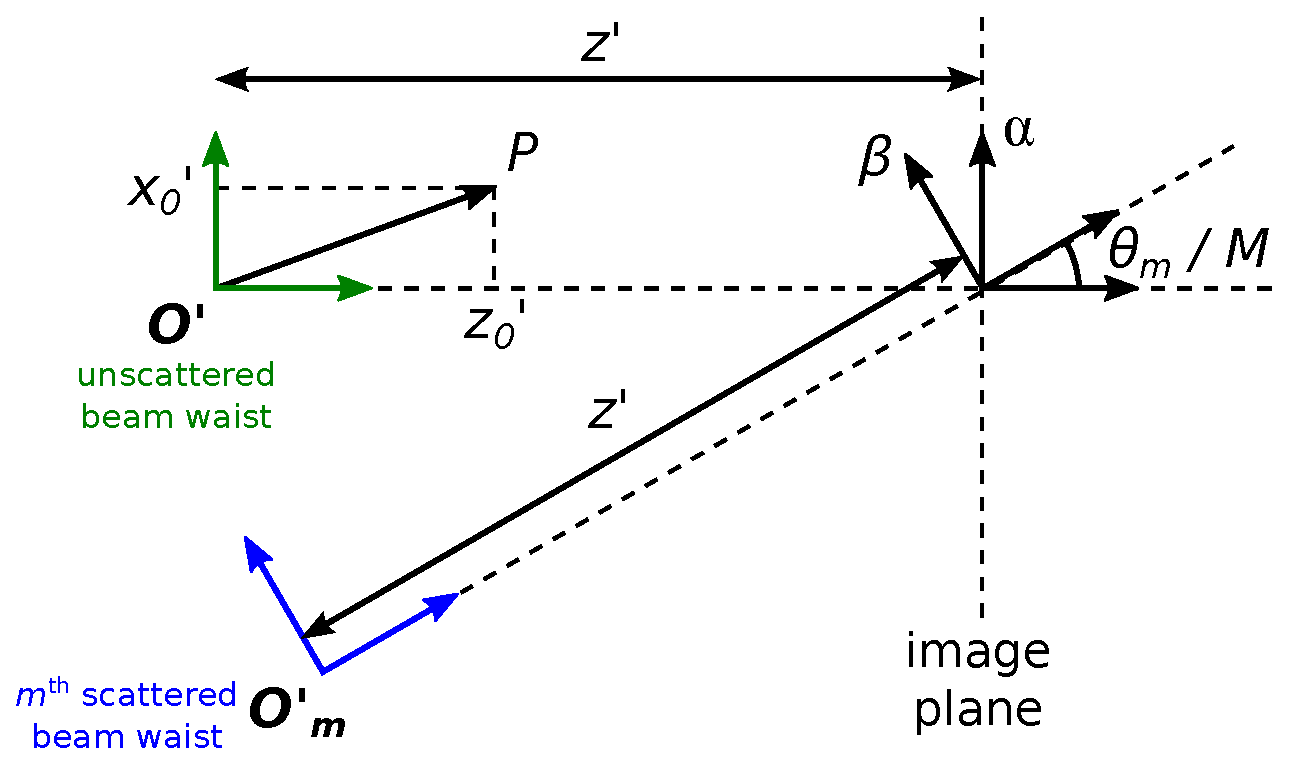
\includegraphics[width = 0.9 \textwidth]{%
    Chapters/InterferometricMethods/figs/coordinate_transformation_imaging_plane.eps}
  \caption[Image-plane coordinate transformation]{%
    Image-plane coordinate transformation}
\label{fig:InterferometricMethods:coordinate_transformation_imaging_plane}
\end{figure}


\subsection{The imaged field}
Now, without further ado,
let $\image$ image the object plane $S_{\object}$
such that the image of diffracted field
(\ref{eq:InterferometricMethods:phase_modulated_Gaussian_beam_diffraction_Fourier_filtered})
is
\begin{align}
  E(\vect{r}_{\image}, t)
  &=
  \image[ E(\vect{r}_{\object}, t) ]
  \notag \\
  &=
  e^{i \bar{\phi}}
  \sum_{m = -\infty}^{\infty}
  i^m \left[ J_m(\tilde{\phi}_0) \right]
  \image[\mathcal{E}_G(\vect{r}_{m,\object})]
  e^{-i (\omega_0 + m \omega) t}
  \label{eq:InterferometricMethods:imaged_total_field_v1}
\end{align}
where the linearity of $\image$ has been invoked
to bring the operator within the summation.
Referencing
(\ref{eq:InterferometricMethods:mth_diffracted_beam_kx_filtered_compact}),
it readily follows that
\begin{align}
  \image[\mathcal{E}_G(\vect{r}_{m,\object})]
  &=
  \mathcal{I}[%
    E_G(0, y_{\object}, z_{\object})
    \cdot
    \mathcal{P}(m, k, x_{\object})
  ]
  \notag \\
  &=
  E_G(0, y_{\image}, z_{\image})
  \cdot
  \mathcal{P}(m, k_{\image}, x_{\image})
\end{align}
where the object-plane wavevector $k$ has been imaged as
\begin{equation}
  k_{\image} = \frac{k}{M}
\end{equation}
Thus, (\ref{eq:InterferometricMethods:imaged_total_field_v1}) becomes
\begin{equation}
  \begin{aligned}
    E(\vect{r}_{\image}, t)
    &=
    E_G(0, y_{\image}, z_{\image}, t)
    e^{i \bar{\phi}}
    \\
    &\quad \times
    \sum_{m = -\infty}^{\infty}
    i^m \left[ J_m(\tilde{\phi}_0) \right]
    \mathcal{P}(m, k_{\image}, x_{\image})
    e^{-i m \omega t}
  \end{aligned}
  \label{eq:InterferometricMethods:imaged_total_field}
\end{equation}
where
$E_G(0, y_{\image}, z_{\image}, t)
=
E_G(0, y_{\image}, z_{\image}) e^{-i \omega_0 t}$.


\subsection{The weak-coupling limit}
Typically, the phase-fluctuation amplitude
is very small ($\tilde{\phi}_0 \ll 1$), and
the Bessel function's small-argument limiting form \cite{abramowitz_and_stegun}
can be used
\begin{equation}
  \lim_{z \rightarrow 0} J_m(z)
  \sim
  \begin{cases}
    \frac{1}{\Gamma(m + 1)} \left( \frac{z}{2} \right)^m
    , \qquad
    &m = 0, 1, 2, 3, \cdots
    \\
    \frac{1}{\Gamma(|m| + 1)} \left( \frac{-z}{2} \right)^{|m|}
    , \qquad
    &m = -1, -2, -3, \cdots
  \end{cases}
\end{equation}
Here, $\Gamma$ is the gamma function, and
$\Gamma(m + 1) = m!$ for positive integer $m$.
Dropping terms exceeding first order in $\tilde{\phi}_0$ and
introducing the notational shorthand
$\mathcal{P}_m \equiv \mathcal{P}(m, k_{\image}, x_{\image})$,
(\ref{eq:InterferometricMethods:imaged_total_field}) becomes
\begin{equation}
  \begin{aligned}
  E(\vect{r}_{\image}, t)
  &\approx
  E_G(0, y_{\image}, z_{\image}, t)
  e^{i \bar{\phi}}
  \\
  &\quad\times
  \biggl\{%
    \mathcal{P}_{0}
    +
    i \frac{\tilde{\phi}_0}{2}
    \left[
      \mathcal{P}_{1} e^{-i \omega t}
      +
      \mathcal{P}_{-1} e^{i \omega t}
    \right]
  \biggr\}
  \end{aligned}
  \label{eq:InterferometricMethods:imaged_total_field_weak_coupling_Fourier_filtered}
\end{equation}

It is enlightening to examine the case where there is
no wavenumber-dependent manipulation of the scattered beams
(i.e.\ $T(k_x) = 1$), for which
the phase factor $\mathcal{P}(m, k_{\image}, x_{\image})$ readily reduces to
\begin{equation}
  \mathcal{P}(m, k_{\image}, x_{\image})
  =
  \exp\left[\frac{-x_{m,\image}^2}{w(z_{\image})^2} \right]
  \exp\left\{%
    i \left[%
      m k_{\image} x_{m,\image}
      +
      \frac{k_0 x_{m,\image}^2}{2 R(z_{\image})}
    \right]
  \right\}
\end{equation}
Now, the image-plane coordinate transformation
from $x_{m,\image}$ to $x_{\image}$ is given by
(\ref{eq:InterferometricMethods:coordinate_transformation_imaging_plane}).
Neglecting the small variation in the Gaussian envelope and
retaining phase factors only to second order in $k$ yields
\begin{equation}
  \begin{aligned}
  \mathcal{P}(m, k_{\image}, x_{\image})
  &\approx
  \exp\left[\frac{-x_{\image}^2}{w(z_{\image})^2} \right]
  \exp\left[ \frac{i k_0 x_{\image}^2}{2 R(z_{\image})} \right]
  \\
  &\quad \times
  \exp\left\{%
    i \left[%
      m k_{\image} x_{\image}
      -
      \frac{(m k_{\image} x_{\image})^2}{2 k_0 R(z_{\image})}
    \right]
  \right\}
  \end{aligned}
  \label{eq:InterferometricMethods:mth_diffracted_beam_no_kx_filter_phase_factor}
\end{equation}
Here, the top line corresponds to
the Gaussian envelope and phase-front curvature
of the unscattered ($m = 0$) beam, whereas
the second line corresponds to interference effects.
Substituting
(\ref{eq:InterferometricMethods:mth_diffracted_beam_no_kx_filter_phase_factor})
into
(\ref{eq:InterferometricMethods:imaged_total_field_weak_coupling_Fourier_filtered})
yields
\begin{equation}
  E(\vect{r}_{\image}, t)
  =
  E_G(\vect{r}_{\image}, t)
  e^{i \bar{\phi}}
  \left[%
    1
    +
    i \tilde{\phi}_0 e^{-i \kappa} \cos\xi
  \right]
\end{equation}
where
\begin{align}
  \xi
  &\equiv
  \frac{k x_{\image}}{M} - \omega t
  \label{eq:InterferometricMethods:image_plane_xi}
  \\
  \kappa
  &\equiv
  \frac{1}{2 k_0 R(z_{\image})}
  \left( \frac{k x_{\image}}{M} \right)^2
  \label{eq:InterferometricMethods:image_plane_kappa}
\end{align}
Note that the above definitions have used the substitution
$k_{\image} x_{\image} = k x_{\image} / M$.
Normally, $\kappa \ll 1$ such that the total imaged field reduces to
\begin{equation}
  E(\vect{r}_{\image}, t)
  \approx
  E_G(\vect{r}_{\image}, t)
  e^{i \bar{\phi}}
  \left[%
    1
    +
    i \tilde{\phi}_0 \cos\xi
  \right]
  \label{eq:InterferometricMethods:imaged_total_field_weak_coupling}
\end{equation}


\subsection{The need for a reference beam}
\label{sec:InterferometricMethods:imaging:need_for_reference_beam}
Assume that there is
no wavenumber-dependent manipulation of the diffracted beams
such that
(\ref{eq:InterferometricMethods:imaged_total_field_weak_coupling}) applies.
Now, most detectors of interest are square-law detectors
in that they produce a response proportional to
the square (i.e.\ intensity) of the incident field.
If such a detector is placed at the image plane,
the local intensity is
\begin{align}
  I(\vect{r}_{\image}, t)
  &\equiv
  \frac{c \varepsilon_0}{2} |E(\vect{r}_{\image}, t)|^2
  \notag \\
  &=
  I_G(\vect{r}_{\image})
  [1 + \mathcal{O}(\tilde{\phi}_0)^2]
  \label{eq:InterferometricMethods:imaged_field_intensity}
\end{align}
where
\begin{equation}
  I_G(\vect{r}_{\image})
  =
  \frac{c \varepsilon_0 |E_G(\vect{r}_{\image})|^2}{2}
  \label{eq:InterferometricMethods:Gaussian_beam_intensity}
\end{equation}
is the intensity profile (averaged over an optical cycle)
of the undiffracted Gaussian beam.
Thus, for the typical $\tilde{\phi}_0 \ll 1$ limit,
the measured response will be very weak
if the detector is only exposed to the imaged radiation.
Physically, this is attributable to the $m = \pm 1$ beams
being $\pi / 2$ out of phase with the unscattered $m = 0$ beam.
As will be shown in Sections
\ref{sec:InterferometricMethods:interferometry} and
\ref{sec:InterferometricMethods:pci},
the system response can be substantially improved
by interfering the scattered beams with a reference beam.
The generation of such a reference beam, then, is the trait
that differentiates a given interferometric method from another.


\section{External reference-beam interferometry}
\label{sec:InterferometricMethods:interferometry}
In external reference-beam interferometry,
there is no wavenumber-dependent manipulation of the diffracted beams
such that
(\ref{eq:InterferometricMethods:imaged_total_field_weak_coupling}) applies.
Thus, the probe radiation in the image plane is given as
\begin{equation}
  E_P(\vect{r}_{\image}, t)
  \approx
  E_G(\vect{r}_{\image}, t)
  e^{i \bar{\phi}}
  \left[%
    1
    +
    i \tilde{\phi}_0 \cos\xi
  \right]
\end{equation}
Now, assume that the imaged probe radiation
is interfered with a reference beam of known phase $\phi_R$
\begin{equation}
  E_R(\vect{r}_{\image}, t) = E_G(\vect{r}_{\image}, t) e^{i \phi_R}
  \label{eq:InterferometricMethods:external_reference_beam_arbitrary}
\end{equation}
The total field impinging on the detector is then
\begin{equation}
  E(\vect{r}_{\image}, t)
  =
  E_G(\vect{r}_{\image}, t)
  \left[%
    e^{i \phi_R}
    +
    e^{i \bar{\phi}}
    \left(%
      1
      +
      i \tilde{\phi}_0 \cos\xi
    \right)
  \right]
\end{equation}
and, to first order in $\tilde{\phi}_0$, the corresponding intensity is
\begin{equation}
  I(\vect{r}_{\image}, t)
  =
  2 I_G(\vect{r}_{\image})
  \left[%
    1
    +
    \cos(\phi_R - \bar{\phi})
    +
    \tilde{\phi}_0 \sin(\phi_R - \bar{\phi}) \cos\xi
  \right]
  \label{eq:InterferometricMethods:interferometer_intensity_arbitrary_reference}
\end{equation}
where $I_G(\vect{r}_{\image})$ is
the intensity profile of the undiffracted Gaussian beam on the detector
as defined in (\ref{eq:InterferometricMethods:Gaussian_beam_intensity}).
Reference-beam generation prescribes $\phi_R$ and
consequently dictates the method of interferometric detection.


\subsection{Homodyne detection}
\label{sec:InterferometricMethods:interferometry:homodyne}
\begin{figure}
  \centering
  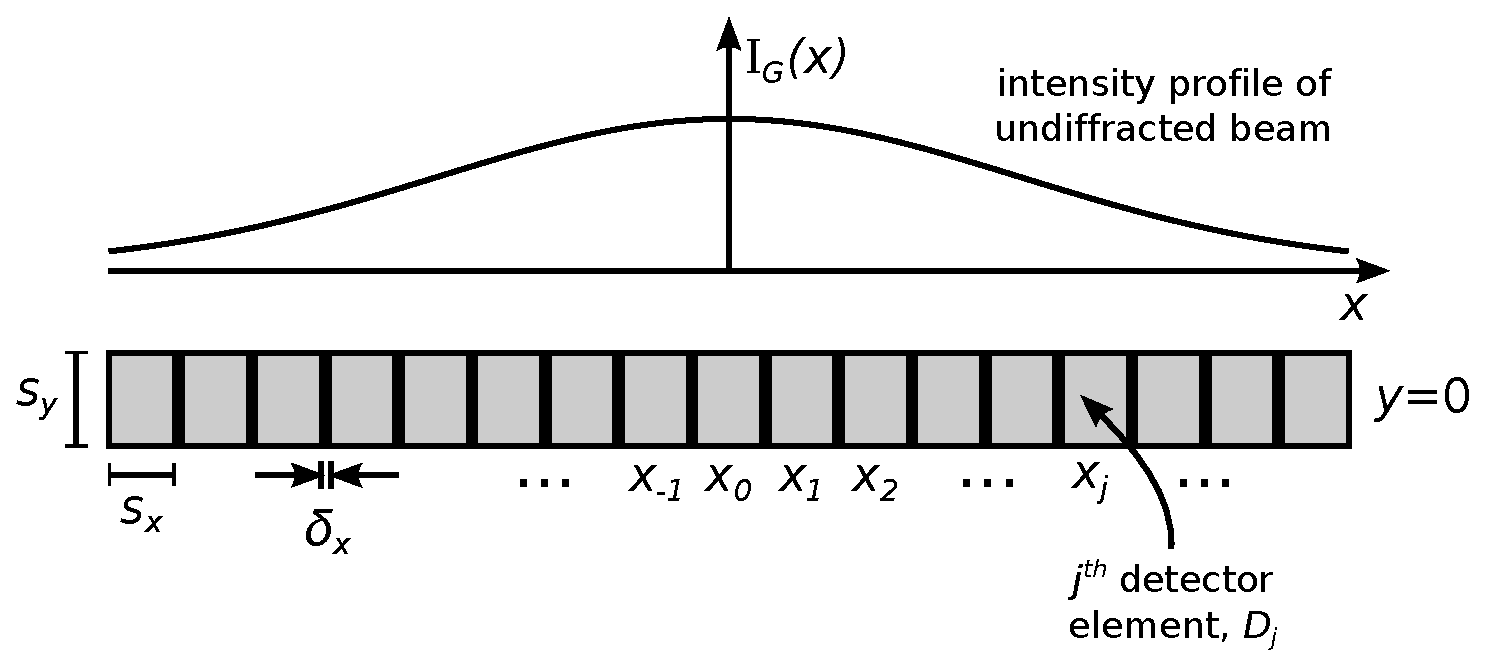
\includegraphics[width = \textwidth]{%
    Chapters/InterferometricMethods/figs/detector_array.eps}
  \caption[Finite sampling-volume effects in a detector array]{%
    The probe radiation and the reference beam
    are interfered on a detector array.
    The array consists of numerous detector elements,
    each of size $s_x \times s_y$ and with interelement spacing $\delta_x$.
    The undiffracted beam is centered on $x_0 = 0$ and $y = 0$, and
    its intensity profile varies only weakly over any given element.
    The finite size of each detector element tends to attenuate
    short wavelength components of the incident optical signal.
  }
  \label{fig:InterferometricMethods:detector_array}
\end{figure}

Homodyne detection results from using
a reference phase that is constant (or nearly constant) in time
such that the resulting intensity is
\begin{equation}
  \begin{aligned}
    I_{\text{hom}}(\vect{r}_{\image}, t)
    =
    2 I_G(\vect{r}_{\image})
    \bigl[%
      1
      &+
      \cos(\phi_R - \bar{\phi})
      \\
      &+
      \tilde{\phi}_0
      \sin(\phi_R - \bar{\phi}) \cos\xi
    \bigr]
  \end{aligned}
  \label{eq:InterferometricMethods:homodyne_intensity}
\end{equation}
Finite sampling-volume effects~\cite{bravenec_rsi95} dictate
the homodyne interferometer's wavenumber response~\cite{davis_rsi16}.
Assume that the probe radiation and the reference beam
are interfered on a detector array,
as shown in Fig.~\ref{fig:InterferometricMethods:detector_array}.
Let the $j$\ts{th} detector element $D_j$ be centered on $x_{\image,j}$
and $y_{\image} = 0$;
the total power $P_{j, \, \text{hom}}$ incident on this element is then
\begin{align}
  P_{j, \, \text{hom}}(t)
  &=
  \int_{D_j} I_{\text{hom}}(\vect{r}_{\image}, t) dA
  \notag \\
  &\begin{aligned}
    \approx
    2 I_G(\vect{r}_{\image,j}) s_y
    \int_{x_{\image,j} - s_x / 2}^{x_{\image,j} + s_x / 2}
    \bigl[%
      1
      &+
      \cos(\phi_R - \bar{\phi})
      \\
      &+
      \tilde{\phi}_0
      \sin(\phi_R - \bar{\phi}) \cos\xi
    \bigr] dx_{\image}
  \end{aligned}
  \notag
\end{align}
where the weakly varying intensity profile $I_G(\vect{r}_{\image})$
has been approximated as a constant
over the face of the detector element.
As the finite sampling-volume integral
will also be applied in other sections,
it is explicitly evaluated here for later reference
\begin{equation}
  \int_{x_{\image,j} - s_x / 2}^{x_{\image,j} + s_x / 2}
  \cos(\xi + \theta) dx_{\image}
  =
  s_x
  \cdot
  T_{\text{fsv}}(k)
  \cdot
  \cos(\xi_j + \theta)
  \label{eq:InterferometricMethods:finite_sampling_volume_integral}
\end{equation}
where
\begin{equation}
  T_{\text{fsv}}(k)
  \equiv
  \sinc\left( \frac{k}{k_c} \right)
  \label{eq:InterferometricMethods:finite_sampling_volume_transfer_function}
\end{equation}
is the finite sampling-volume transfer function
\begin{equation}
  \sinc(x) = \frac{\sin(\pi x)}{\pi x}
  \label{eq:InterferometricMethods:normalized_sinc}
\end{equation}
is the normalized sinc function,
\begin{equation}
  k_c = \frac{2 \pi M}{s_x}
  \label{eq:InterferometricMethods:finite_sampling_volume_cutoff}
\end{equation}
is the first zero (i.e.\ ``cutoff'') of $T_{\text{fsv}}(k)$,
\begin{equation}
  \xi_j = \frac{k x_{\image,j}}{M} - \omega t
  \label{eq:InterferometricMethods:xi_j}
\end{equation}
and $\theta$ is a \emph{constant} with respect to $x_{\image}$.
Thus, the homodyne optical power becomes
\begin{align}
  \begin{aligned}
    P_{j, \, \text{hom}}(t)
    =
    2 I_G(\vect{r}_{\image,j}) A
    &\bigl[%
      1
      +
      \cos(\phi_R - \bar{\phi})
      \\
      &+
      \tilde{\phi}_0
      \sin(\phi_R - \bar{\phi})
      T_{\text{fsv}}(k)
      \cos\xi_j
    \bigr]
  \end{aligned}
  \label{eq:InterferometricMethods:homodyne_interferometer_total_power_per_element}
\end{align}
where $A = s_x s_y$ is the area of the detector element.

The typical engineering constraint of such a system
is the saturation intensity of the detector elements.
Beyond the linear saturation intensity $I_{\text{sat}}$,
the detector's response ceases to be a linear function
of the incident optical power.
For approximately uniform illumination,
the saturation threshold can be equivalently characterized
by a saturation power $P_{\text{sat}} \equiv I_{\text{sat}} A$.
To make an ``apples-to-apples'' comparison of different interference schemes,
it is useful to examine the ratio of the fluctuating power to $P_{\text{sat}}$.
To proceed, note that the homodyne optical power in
(\ref{eq:InterferometricMethods:homodyne_interferometer_total_power_per_element})
can be separated into equilibrium and fluctuating components as
$P_{j, \, \text{hom}}(t)
=
\bar{P}_{j, \, \text{hom}}
+
\tilde{P}_{j, \, \text{hom}}(t)$, where
\begin{align}
  \bar{P}_{j, \, \text{hom}}(t)
  &=
  2 I_G(\vect{r}_{\image,j}) A
  [1 + \cos(\phi_R - \bar{\phi})]
  \\
  \tilde{P}_{j, \, \text{hom}}(t)
  &=
  2 I_G(\vect{r}_{\image,j}) A
  \tilde{\phi}_0
  \sin(\phi_R - \bar{\phi})
  T_{\text{fsv}}(k)
  \cos\xi_j
\end{align}
Then, because $\tilde{\phi}_0 \ll 1$
\begin{equation}
  P_{j, \, \text{hom}}
  \approx
  \bar{P}_{j, \, \text{hom}}
  \leq
  2 I_G(0) A [1 + \cos(\phi_R - \bar{\phi})]
  \notag
\end{equation}
where $I_G(0)$ is the peak intensity of the undiffracted Gaussian probe beam.
To obtain optimal performance, select $I_G(0)$ such that
\begin{equation}
  P_{\text{sat}}
  =
  2 I_G(0) A [1 + \cos(\phi_R - \bar{\phi})]
  \notag
\end{equation}
Then
\begin{equation}
  \frac{\tilde{P}_{j, \, \text{hom}}(t)}{P_{\text{sat}}}
  =
  \frac{I_G(\vect{r}_{\image,j})}{I_G(0)}
  \cdot
  T_{\text{hom}}(k)
  \cdot
  \tilde{\phi}_0 \cos\xi_j
\end{equation}
where
\begin{equation}
  T_{\text{hom}}(k)
  \equiv
  \frac{\sin(\phi_R - \bar{\phi})}{1 + \cos(\phi_R - \bar{\phi})}
  \cdot
  T_{\text{fsv}}(k)
  \label{eq:InterferometricMethods:homodyne_interferometer_wavenumber_transfer_function}
\end{equation}
is the homodyne interferometer's wavenumber transfer function.
That is, the homodyne interferometer
weights the phase-fluctuation images $\tilde{\phi}_0 \cos\xi_j$
by its transfer function $T_{\text{hom}}(k)$.
The prefactor $I_G(\vect{r}_{\image,j}) / I_G(0)$
can (and should) be accounted for
if the beam profile is known.

Note that $T_{\text{hom}}(k)$ is a function
of the phase difference $\phi_R - \bar{\phi}$.
The homodyne interferometer operates at its peak sensitivity
when $|T_{\text{hom}}(k)|$ is maximal,
which occurs when $\phi_R - \bar{\phi} = \pi / 2 + m \pi$ for integer $m$.
For concreteness in the following discussion,
take $\phi_R - \bar{\phi} = \pi / 2$.
Physically, $\phi_R - \bar{\phi} = \pi / 2$
means that the reference beam is
out-of-phase with the undiffracted beam but
in-phase with the diffracted beams.
Note that interfering the diffracted beams with this in-phase reference beam
produces an intensity linear in $\tilde{\phi}_0$;
this should be contrasted with the situation
that produces the weak, quadratic intensity variation in
(\ref{eq:InterferometricMethods:imaged_field_intensity}).

Practically speaking, however,
it is very difficult to keep $\phi_R - \bar{\phi}$ fixed at $\pi / 2$.
First, a CO$_2$ beam passing through $\sim \SI{1}{\meter}$
of plasma with a density $n_e \sim \SI{e20}{\per\meter\cubed}$
will experience a bulk phase delay $\bar{\phi} \sim \pi$;
thus, for constant $\phi_R$, it will be impossible
to operate the interferometer at its peak sensitivity
($\phi_R - \bar{\phi} \approx \pi / 2$)
as the density evolves across the discharge.
Second, fusion experiments are often characterized
by large, pulsed electromagnets
whose vibrations can change the path lengths of the interferometer's arms.
A path-length change $\delta l$ produces
$\delta(\phi_R - \bar{\phi}) = k_0 \delta l$,
where $k_0$ is the wavenumber of the probe radiation.
For a $\SI{10.6}{\micro\meter}$ CO$_2$ probe beam,
a path-length variation $\sim \SI{2.5}{\micro\meter}$
is sufficient to produce $\delta(\phi_R - \bar{\phi}) \sim \pi / 2$,
pushing the homodyne interferometer from
its configuration of peak sensitivity into one of its nulls.
Even vacuum-pump vibrations can provide such a push!
On small fusion devices,
actively controlled mirrors have been used in an attempt
to account for the evolution of the equilibrium phase and
to cancel vibrational path-length changes,
minimizing excursions from $\phi_R - \bar{\phi} \approx \pi / 2$
\cite{nazikian_rsi87}, but
such an approach has not found application on larger
(and presumably more vibration-prone) fusion experiments.

In addition to its variable sensitivity,
the homodyne interferometer does \emph{not} make an absolute measurement
of the phase fluctuation amplitude $\tilde{\phi}_0$
\cite[Sec.~4.2.2]{hutchinson_diagnostics}.
For example, vibration-induced misalignment or
power fluctuations at the beam source
can alter the intensity $I_G(\vect{r}_{\image,j})$.
As a result, there are three potentially dynamic quantities:
$\{\phi_R - \bar{\phi}, \tilde{\phi}_0, I_G(\vect{r}_{\image,j})\}$, but
there are only two measured quantities:
the equilibrium and fluctuating homodyne powers.
Thus, it is generally impossible to distinguish
whether changes in the amplitude of the fluctuating power
are attributable to real changes in $\tilde{\phi}_0$ or
are simply an artifact of the system alignment or radiation source.


\subsection{Heterodyne detection}
\graffito{\textcolor{blue}{Qualitative figure of baseband vs IF}}
To avoid the above-mentioned challenges of homodyne interferometry,
the reference phase can be linearly ramped in time
as $\phi_R = \Delta \omega_0 t$ such that
the intensity becomes
\begin{equation}
  \begin{aligned}
    I_{\text{het}}(\vect{r}_{\image}, t)
    =
    2 I_G(\vect{r}_{\image})
    \bigl[%
      1
      &+
      \cos(\Delta \omega_0 t - \bar{\phi})
      \\
      &+
      \tilde{\phi}_0
      \sin(\Delta \omega_0 t - \bar{\phi}) \cos\xi
    \bigr]
  \end{aligned}
  \label{eq:InterferometricMethods:heterodyne_intensity}
\end{equation}
This approach is known as heterodyne interferometry,
as the desired baseband phase information is shifted
to an intermediate frequency $\Delta \omega_0$
satisfying $(d\phi/dt)_{\text{max}} \ll \Delta \omega_0 \ll \omega_0$.
\graffito{\textcolor{red}{This will be discussed more in Ch.~3}}
Practically, the $\phi_R$ ramp is accomplished by modestly Doppler shifting
the reference beam relative to the plasma beam.

As is the case for homodyne detection,
finite sampling-volume effects~\cite{bravenec_rsi95} dictate
the heterodyne interferometer's wavenumber response~\cite{davis_rsi16}.
The following discussion closely parallels that
of the homodyne interferometer in
Section~\ref{sec:InterferometricMethods:interferometry:homodyne}, and
readers are encouraged to review that section if needed and
to compare and contrast homodyne and heterodyne detection.
Assume that the probe radiation and the reference beam
are interfered on a detector array,
as shown in Fig.~\ref{fig:InterferometricMethods:detector_array}.
Let the $j$\ts{th} detector element $D_j$ be centered on $x_j$ and $y = 0$;
the total power $P_{j, \, \text{het}}$ incident on this element is then
\begin{align}
  P_{j, \, \text{het}}(t)
  &=
  \int_{D_j} I_{\text{het}}(\vect{r}_{\image}, t) dA
  \notag \\
  &\begin{aligned}
    \approx
    2 I_G(\vect{r}_{\image,j}) s_y
    \int_{x_{\image,j} - s_x / 2}^{x_{\image,j} + s_x / 2}
    \bigl[%
      1
      &+
      \cos(\Delta \omega_0 t - \bar{\phi})
      \\
      &+
      \tilde{\phi}_0
      \sin(\Delta \omega_0 t - \bar{\phi}) \cos\xi
    \bigr] dx
  \end{aligned}
  \notag \\
  &\begin{aligned}
    =
    2 I_G(\vect{r}_{\image,j}) A
    \bigl[%
      &1
      +
      \cos(\Delta \omega_0 t - \bar{\phi})
      \\
      &+
      \tilde{\phi}_0
      \sin(\Delta \omega_0 t - \bar{\phi})
      T_{\text{fsv}}(k)
      \cos\xi_j
    \bigr]
  \end{aligned}
  \label{eq:InterferometricMethods:heterodyne_interferometer_total_power_per_element}
\end{align}
where the weakly varying intensity profile $I_G(\vect{r}_{\image})$
has been approximated as a constant
over the face of the detector element, and
the finite sampling-volume integral in
(\ref{eq:InterferometricMethods:finite_sampling_volume_integral})
has been referenced.
Note that the dominant Fourier components of $P_{j, \, \text{het}}$
sit at the intermediate frequency $\pm \Delta \omega_0$ but that
the phase-fluctuation term $\sin(\Delta \omega_0 t - \bar{\phi}) \cos\xi_j$
produce sidebands at $\pm (\Delta \omega_0 \pm \omega)$.

The heterodyne interference signal must be demodulated
in order to retrieve the baseband phase-fluctuation information.
\graffito{\textcolor{red}{More on demodulation hardware in Ch.~3}}
Practically speaking, dedicated analog or digital electronics
are used to demodulate the heterodyne signal;
however, for the pedagogical purposes of this section,
it is sufficient to consider the ``equivalent optical powers''
corresponding to the demodulated signals.
The so-called in-phase ($I$) and quadrature ($Q$) signals
are obtained by mixing $P_{j, \, \text{het}}$ with
$\cos( \Delta \omega_0 t)$ and $\sin( \Delta \omega_0 t)$, respectively, and
low-pass filtering the resulting signals;
here, low-pass filtering is implemented
by averaging over a cycle of the intermediate frequency.
Thus, the equivalent $I$ and $Q$ optical powers are defined as
\begin{align}
  P_{j, I}(t)
  &\equiv
  \langle
    \cos (\Delta \omega_0 t) \cdot P_{j, \, \text{het}}(t)
  \rangle_{\Delta \omega_0}
  \\
  P_{j, Q}(t)
  &\equiv
  \langle
    \sin (\Delta \omega_0 t) \cdot P_{j, \, \text{het}}(t)
  \rangle_{\Delta \omega_0}
\end{align}
where $\langle q \rangle_{\Delta \omega_0}$ denotes
the average of quantity $q$ over an intermediate-frequency cycle as
\begin{equation}
  \langle q \rangle_{\Delta \omega_0}
  \equiv
  \frac{\Delta \omega_0}{2 \pi}
  \int_{0}^{\Delta \omega_0 / 2 \pi}
  q(t) dt
  \label{eq:InterferometricMethods:intermediate_frequency_cycle_average}
\end{equation}
Note that $P_{j,I}$ and $P_{j,Q}$ can be conveniently combined as
\begin{align}
  P_{j,I} + i \cdot P_{j,Q}
  &=
  \langle
    e^{i \Delta \omega_0 t} \cdot P_{j, \, \text{het}}(t)
  \rangle_{\Delta \omega_0}
  \notag \\
  &=
  I_G(\vect{r}_{\image,j}) A
  e^{i \bar{\phi}}
  \left[%
    1
    +
    i \tilde{\phi}_0
    T_{\text{fsv}}(k)
    \cos\xi_j
  \right]
  \label{eq:InterferometricMethods:heterodyne_interferometer_I_and_Q_power_per_element}
\end{align}

In contrast to the homodyne interferometer,
the heterodyne interferometer makes an absolute measurement
of the phase-fluctuation amplitude $\tilde{\phi}_0$.
To see this, note that $P_{j,I}$ and $P_{j,Q}$ in
(\ref{eq:InterferometricMethods:homodyne_interferometer_total_power_per_element})
can be separated into equilibrium and fluctuating components as
\begin{align}
  \bar{P}_{j,I}(t)
  &=
  I_G(\vect{r}_{\image,j}) A \cos\bar{\phi}
  \\
  \bar{P}_{j,Q}(t)
  &=
  I_G(\vect{r}_{\image,j}) A \sin\bar{\phi}
  \\
  \tilde{P}_{j,I}(t)
  &=
  -I_G(\vect{r}_{\image,j}) A
  \tilde{\phi}_0
  \sin\bar{\phi} \,
  T_{\text{fsv}}(k)
  \cos\xi_j
  \\
  \tilde{P}_{j,Q}(t)
  &=
  I_G(\vect{r}_{\image,j}) A
  \tilde{\phi}_0
  \cos\bar{\phi} \,
  T_{\text{fsv}}(k)
  \cos\xi_j
\end{align}
As is the case for the homodyne interferometer,
there are three potentially dynamic quantities:
$\{\bar{\phi}, \tilde{\phi}_0, I_G(\vect{r}_{\image,j})\}$;
however, in contrast to the homodyne interferometer,
there are now \emph{four} measured quantities:
$\{\bar{P}_{j,I}, \bar{P}_{j,Q}, \tilde{P}_{j,I}, \tilde{P}_{j,Q}\}$.
Therefore, the number of measured quantities
is sufficient to unambiguously determine
$\{\bar{\phi}, \tilde{\phi}_0, I_G(\vect{r}_{\image,j})\}$
in absolute units.

Finally, it is useful to characterize
the heterodyne interferometer's performance
relative to the saturation limits of a given detector.
Because $\tilde{\phi}_0 \ll 1$,
(\ref{eq:InterferometricMethods:heterodyne_interferometer_total_power_per_element})
can be approximated as
\begin{align}
  P_{j, \, \text{het}}
  &\approx
  2 I_G(\vect{r}_{\image,j}) A [1 + \cos(\Delta \omega_0 t - \bar{\phi})]
  \notag \\
  &\leq
  4 I_G(0) A
  \notag
\end{align}
where $I_G(0)$ is the peak intensity of the undiffracted Gaussian probe beam.
To obtain optimal performance, select $I_G(0)$ such that
\begin{equation}
  P_{\text{sat}}
  =
  4 I_G(0) A
  \notag
\end{equation}
Further, define the total fluctuating power
in the demodulated signals to be
\begin{align}
  \tilde{P}_{j, IQ}(t)
  &\equiv
  \left\{%
    [\tilde{P}_{j,I}(t)]^2
    +
    [\tilde{P}_{j,Q}(t)]^2
  \right\}^{1/2}
  \notag \\
  &=
  I_G(\vect{r}_{\image,j}) A
  \tilde{\phi}_0
  T_{\text{fsv}}(k)
  \cos\xi_j
\end{align}
such that
\begin{equation}
  \frac{\tilde{P}_{j, IQ}(t)}{P_{\text{sat}}}
  =
  \frac{I_G(\vect{r}_{\image,j})}{I_G(0)}
  \cdot
  T_{\text{het}}(k)
  \cdot
  \tilde{\phi}_0
  \cos\xi_j
\end{equation}
where
\begin{equation}
  T_{\text{het}}(k)
  \equiv
  \frac{T_{\text{fsv}}(k)}{4}
  \label{eq:InterferometricMethods:heterodyne_interferometer_wavenumber_transfer_function}
\end{equation}
is the heterodyne interferometer's wavenumber transfer function.
That is, the heterodyne interferometer
weights the phase-fluctuation images $\tilde{\phi}_0 \cos\xi_j$
by its transfer function $T_{\text{het}}(k)$.
The prefactor $I_G(\vect{r}_{\image,j}) / I_G(0)$
can (and should) be accounted for
if the beam profile is known.

In contrast to the homodyne interferometer,
the heterodyne interferometer's wavenumber transfer function
is \emph{not} a function of $\phi_R - \bar{\phi}$.
Thus, the heterodyne interferometer always operates at its peak sensitivity,
regardless of the bulk plasma phase or path-length vibrations.
Robust sensitivity comes at a cost, however.
Note that
\begin{equation}
  \frac{T_{\text{het}}(k)}{T_{\text{hom}}(k)}
  =
  \frac{1}{4}
  \quad
  \text{for homodyne operation at $\phi_R - \bar{\phi} = \pi / 2$}
  \notag
\end{equation}
Thus, for a given detector,
a heterodyne interferometer will be four times \emph{less} sensitive
than a homodyne interferometer operated in its optimal configuration
($\phi_R - \bar{\phi} = \pi / 2$).
This factor of four has two physical origins.
First, the detector of a homodyne interferometer
with a fixed $\phi_R - \bar{\phi} = \pi / 2$
only sees small fluctuations about a DC offset, while
the detector of a heterodyne interferometer
sees the full sinusoidal waveform of the intermediate frequency;
to ensure the detector is always within its saturation limits,
the heterodyne interferometer must necessarily be operated with
a mean intensity at the detector
that is a factor of two lower than that for the homodyne interferometer.
Second, the mixing process
that is used to demodulate the heterodyne interference signal
results in a loss of half of the signal power.


\section{Phase contrast imaging (PCI)}
\label{sec:InterferometricMethods:pci}
As discussed in
Section~\ref{sec:InterferometricMethods:imaging:need_for_reference_beam},
imaging the probe radiation on a square-law detector
produces a very weak response
because the undiffracted and diffracted beams
are $\pi / 2$ out of phase with each other.
To produce a measurable response, a traditional interferometer
interferes the imaged radiation with an external reference beam.
If the phase of the undiffracted beam could be manipulated, though,
the external reference beam would no longer be needed.
This is the approach employed in phase contrast imaging (PCI).


\subsection{Reference-beam generation with a phase plate}
PCI uses an optical element known as a \emph{phase plate}
to delay the undiffracted beam by $\pi / 2$
relative to the diffracted beams.
The phase plate is typically a reflective optical element
with a groove that is precisely fabricated
to have a depth of $\lambda_0 / 8$;
the undiffracted beam reflects off of this groove, and
the corresponding $\lambda_0 / 4$-increase in path length
phase delays the undiffracted beam by $\pi / 2$
relative to the diffracted beams,
which reflect off of the non-grooved portions of the phase plate.
To boost the relative size of the fluctuating signal,
the phase groove typically reflects only a fraction $\eta < 1$
of the incident undiffracted beam power, while
the non-grooved portions of the phase plate
reflect all of the diffracted beam power.
Thus, by the action of the phase plate,
the electric field in the PCI image plane becomes
\begin{equation}
  E_{\text{PCI}}(\vect{r}, t)
  =
  i E_G(\vect{r}, t) e^{i \bar{\phi}}
  \left[%
    \sqrt{\eta} + \tilde{\phi}_0 \cos\xi
  \right]
  \label{eq:InterferometricMethods:pci_imaged_field}
\end{equation}
and, to first order in $\tilde{\phi}_0$, the corresponding intensity is
\begin{equation}
  I_{\text{PCI}}(\vect{r}, t)
  =
  I_G(\vect{r})
  \left[%
    \eta
    +
    2 \sqrt{\eta} \tilde{\phi}_0 \cos\xi
  \right]
  \label{eq:InterferometricMethods:pci_intensity}
\end{equation}
where $E_G(\vect{r})$ and $I_G(\vect{r})$ would be
the field and intensity profiles
of the undiffracted Gaussian beam on the detector
in the \emph{absence} of the phase plate;
$I_G(\vect{r})$ is defined in
(\ref{eq:InterferometricMethods:Gaussian_beam_intensity}).
Equations
(\ref{eq:InterferometricMethods:pci_imaged_field}) and
(\ref{eq:InterferometricMethods:pci_intensity})
should be contrasted with their corresponding equations
in the absence of the phase plate:
(\ref{eq:InterferometricMethods:imaged_total_field_weak_coupling}) and
(\ref{eq:InterferometricMethods:imaged_field_intensity}), respectively.
Thus, the phase plate converts the undiffracted probe beam
into an effective reference beam for the diffracted beams.


\subsection{Focal-plane separation of diffracted beams}
Implicit in the use of the phase plate
is that the undiffracted and diffracted beams
are well-separated in space
such that the phase groove only affects the undiffracted beam.
The 1\ts{st}-order diffracted beams are angularly separated
from the undiffracted beam by $\theta = k / k_0$.
\graffito{\textcolor{red}{Sufficiently large: $k w_0 \gtrsim 2$?}}
Provided that $\theta$ is sufficiently large,
the diffracted and undiffracted beams
will be spatially separated in the far-field
($z \gg z_R$, with $z_R$ being the Rayleigh length of the in-vessel beam);
however, $z \gg z_R$ is not easily accessed in typical lab settings.
Fortunately, the far-field diffraction pattern
can be equivalently accessed in the focal plane
\graffito{\textcolor{red}{Chapter???}}
of a focusing optic~\cite{born_and_wolf}.

The focal-plane location, beam size, and beam separation
can be easily determined.
Let the Gaussian probe beam have
an in-vessel 1/e $E$ waist radius of $w_0$,
and place a focusing optic of focal length $f$
a distance $s$ downstream from the in-vessel beam waist.
Then, the waist of the focused beam
will be located a distance $s'$ downstream of the focusing optic
and will have 1/e $E$ radius $w_0'$ given as
\begin{align}
  s' &= f \left( 1 + \frac{s - f}{z_R} \right)
  \label{eq:InterferometricMethods:focal_plane_location_general}
  \\
  w_0' &= \frac{w_0 |f|}{\left[ (s - f)^2 + z_R^2 \right]^{1/2}}
  \label{eq:InterferometricMethods:focal_plane_waist_general}
\end{align}
where $z_R$ is the in-vessel Rayleigh length~\cite{self83}.
When $|s - f| \ll z_R$, as is typical for PCI,
(\ref{eq:InterferometricMethods:focal_plane_location_general}) and
(\ref{eq:InterferometricMethods:focal_plane_waist_rayleigh}) become
\graffito{\textcolor{red}{%
  Simple optics gives correct $s'$, but
  Gaussian beam physics needed for $w_0'$}
}%
\begin{align}
  s' &\approx f
  \label{eq:InterferometricMethods:focal_plane_location_rayleigh}
  \\
  w_0' &\approx \frac{2 |f|}{k_0 w_0}
  \label{eq:InterferometricMethods:focal_plane_waist_rayleigh}
\end{align}
The spatial separation $\Delta$
of the diffracted beam from the undiffracted beam
in the focal lane is found through the corresponding ray matrices
\begin{align}
  \begin{pmatrix}
    \Delta
    \\
    \theta_{pp}
  \end{pmatrix}
  &=
  \begin{pmatrix}
    1 & s'
    \\
    0 & 1
  \end{pmatrix}
  \begin{pmatrix}
    1      & 0
    \\
    -1 / f & 1
  \end{pmatrix}
  \begin{pmatrix}
    1 & s
    \\
    0 & 1
  \end{pmatrix}
  \begin{pmatrix}
    0
    \\
    \theta
  \end{pmatrix}
\end{align}
which simplifies to
\begin{equation}
  \Delta
  =
  \frac{k |f|}{k_0}
  \label{eq:InterferometricMethods:phase_plate_beam_separation}
\end{equation}


\subsection{Low-$k$ cutoff of phase plate}
Now, let the phase plate groove have a width $d$.
Finite PCI response requires that (most of) the diffracted beams
fall outside of the phase groove (e.g.\ $\Delta \geq d / 2$
such that at least half of the scattered beam
falls outside of the phase groove).
Application of (\ref{eq:InterferometricMethods:phase_plate_beam_separation})
then shows that there will be finite PCI response
for $k \geq k_g$ where
\begin{equation}
  k_g \equiv \frac{k_0 d}{2 f}
  \label{eq:InterferometricMethods:pci_kmin_engineering}
\end{equation}
Here, the subscript $g$ is in reference
to the \emph{groove} of the phase plate.
Further, the scattering process is usually very weak.
To avoid saturating the detector with the signal from the unscattered beam,
the unscattered beam should fall wholly within the phase groove
($2 w_0' \leq d$), which usually has a reflectivity $\eta \ll 1$.
Application of (\ref{eq:InterferometricMethods:focal_plane_waist_rayleigh})
then yields a constraint on the phase groove width
\begin{equation}
  d \geq \frac{4 |f|}{k_0 w_0}
  \label{eq:InterferometricMethods:phase_groove_constraint}
\end{equation}
and inserting (\ref{eq:InterferometricMethods:phase_groove_constraint}) into
(\ref{eq:InterferometricMethods:pci_kmin_engineering}) yields
\begin{equation}
  k_g \geq \frac{2}{w_0}
  \label{eq:pci_kmin_physics}
\end{equation}
\graffito{\textcolor{red}{%
  Note that this is the same limit as for true far-field spatial separation
  (i.e.\ when not using focal-plane spatial separation)}
}%
That is, PCI's low-$k$ cutoff
is ultimately constrained by the in-vessel beam size $w_0$,
with diffraction being the constraining physical mechanism.


\subsection{High-$k$ cutoff of phase plate}
Let the phase plate have a diameter $D$.
Detection of the diffracted radiation
requires that (most of) the diffracted beam reflect
from the face of the phase plate
(e.g.\ $\Delta \leq D / 2$).
Application of (\ref{eq:InterferometricMethods:phase_plate_beam_separation})
then shows that there will be finite PCI response for $k \leq k_D$ where
\begin{equation}
  k_D \equiv \frac{k_0 D}{2 f}
  \label{eq:InterferometricMethods:pci_kmax_engineering}
\end{equation}


\subsection{Effect of phase plate on $m$\ts{th} scattered beam}
The effect of the PCI phase plate on the $m$\ts{th} scattered beam
is given by the phase factor $\mathcal{P}(m, k, x)$,
which is derived and thoroughly discussed in
Appendix~\ref{app:PCIResponseIdentities}.
The relevant results are briefly summarized here for completeness.
In the image plane, the PCI phase factor readily reduces to
\begin{equation}
  \begin{aligned}
    \mathcal{P}(m, k_{\image}, x_{\image})
    &=
    e^{-[x_{\image} / w(z_{\image})]^2}
    e^{i m k_{\image} x_{\image}}
    \\
    &\quad\times
    \left[%
      F(m, k_{\image}, x_{\image})
      +
      G(m, k_{\image}, x_{\image})
    \right]
  \end{aligned}
  \label{eq:InterferometricMethods:PCI_phase_factor_Hermitian_decomposed}
\end{equation}
where the non-grooved portion of the phase plate (i.e.\ the ``face'')
acts on the $m$\ts{th} scattered beam via $F$, while
the phase-plate groove acts on the $m$\ts{th} scattered beam via $G$.
$F$ and $G$ are themselves defined in
(\ref{eq:PCIResponseIdentities:phase_factor_face}) and
(\ref{eq:PCIResponseIdentities:phase_factor_groove}).
Of particular note, $F$ is Hermitian with respect to $m$
\begin{equation}
  F(-m, k_{\image}, x_{\image}) = F^*(m, k_{\image}, x_{\image})
  \label{eq:InterferometricMethods:mth_beam_interaction_with_face_hermitian}
\end{equation}
while $G$ is anti-Hermitian with respect to $m$
\begin{equation}
  G(-m, k_{\image}, x_{\image}) = -G^*(m, k_{\image}, x_{\image})
  \label{eq:InterferometricMethods:mth_beam_interaction_with_groove_antihermitian}
\end{equation}
These symmetries imply
that $F(0, k_{\image}, x_{\image})$ is purely \emph{real} and
that $G(0, k_{\image}, x_{\image})$ is purely \emph{imaginary}.


\subsection{The imaged field and its intensity}
\label{sec:InterferometricMethods:pci:wavenumber_response}
Introducing the notational shorthand
$F_m \equiv F(m, k_{\image}, x_{\image})$ and
$G_m \equiv G(m, k_{\image}, x_{\image})$,
the weak-coupling ($\tilde{\phi}_0 \ll 1$), image-plane electric field from
(\ref{eq:InterferometricMethods:imaged_total_field_weak_coupling_Fourier_filtered})
readily reduces to
\begin{equation}
  \begin{aligned}
  E(\vect{r}_{\image}, t)
  \approx
  E_G(\vect{r}_{\image}, t)
  e^{i \bar{\phi}}
  \biggl\{%
    F_{0} + G_{0}
    &+
    i \frac{\tilde{\phi}_0}{2}
    \biggl[
      (F_{1} + G_{1}) e^{i \xi}
      \\
      &+
      (F_{-1} + G_{-1}) e^{-i \xi}
    \biggr]
  \biggr\}
  \end{aligned}
\end{equation}
where $\xi$ is defined in (\ref{eq:InterferometricMethods:image_plane_xi}) and
$E_G(\vect{r}_{\image}, t)$ would be the image-plane electric field
of the unscattered beam in the \emph{absence} of the phase plate.
Now, recall that $F$ is Hermitian such that
$F_{-1} = F^{*}_{1}$ and $F_{0} = \real(F_{0})$ and
that $G$ is anti-Hermitian such that
$G_{-1} = -G^{*}_{1}$ and $G_{0} = {i \cdot \imag(G_{0})}$;
using these substitutions, the field further reduces to
\begin{equation}
  \begin{aligned}
    E(\vect{r}_{\image}, t)
    =
    E_G(\vect{r}_{\image}, t)
    e^{i \bar{\phi}}
    \biggl\{%
      &\real(F_0) - \tilde{\phi}_0 \imag(G_1 e^{i \xi})
      \\
      &+
      i \left[ \imag(G_0) + \tilde{\phi}_0 \real(F_1 e^{i \xi}) \right]
    \biggr\}
  \end{aligned}
\end{equation}
and the corresponding intensity, to first order in $\tilde{\phi}_0$, is
\begin{equation}
  \begin{aligned}
    I_{\text{pci}}(\vect{r}_{\image}, t)
    &=
    I_G(\vect{r}_{\image})
    \biggl\{%
      |F_0|^2 + |G_0|^2
      \\
      &
      +
      2 \tilde{\phi}_0
      \bigl[%
        \imag(G_0) \real(F_1 e^{i \xi})
        -
        \real(F_0) \imag(G_1 e^{i \xi})
      \bigr]
    \biggr\}
  \end{aligned}
\end{equation}
where $I_G(\vect{r}_{\image})$
would be the intensity profile (averaged over an optical cycle)
of the unscattered beam in the \emph{absence} of the phase plate.
Using the fact that $e^{i \xi} = \cos\xi + {i \sin\xi}$,
$F_1 = \real(F_1) + {i \cdot \imag(F_1)}$, and
$G_1 = \real(G_1) + {i \cdot \imag(G_1)}$,
the image-plane intensity further reduces to
\begin{equation}
  \begin{aligned}
    I_{\text{pci}}(\vect{r}_{\image}, t)
    &=
    I_G(\vect{r}_{\image})
    \biggl\{%
      |F_0|^2 + |G_0|^2
      \\
      &+
      2 \tilde{\phi}_0
      \left[ \imag(G_0)\real(F_1) - \real(F_0)\imag(G_1) \right] \cos\xi
      \\
      &-
      2 \tilde{\phi}_0
      \left[ \imag(G_0)\imag(F_1) + \real(F_0)\real(G_1) \right] \sin\xi
    \biggr\}
  \end{aligned}
  \label{eq:InterferometricMethods:PCI_image_plane_intensity_linear_combination_of_sine_and_cosine}
\end{equation}
Note that the linear combination
$C_I \cos x - C_Q \sin x$ for real $C_I$, $C_Q$, and $x$
can be rewritten as
\begin{equation}
  C_I \cos x - C_Q \sin x = C \cos(x + \theta)
  \label{eq:InterferometricMethods:linear_combination_of_sine_and_cosine}
\end{equation}
where
\begin{align}
  C &= \left( C_I^2 + C_Q^2 \right)^{1/2}
  \\
  \theta &= \atantwo(C_Q, C_I)
\end{align}
where $\atantwo(C_Q, C_I)$
is the arctangent function of two arguments;
$\atantwo(C_Q, C_I)$ gives the angle
corresponding to a tangent of $C_Q / C_I$,
and the signs of $C_Q$ and $C_I$
are used to determine the correct quadrant.
Taking inspiration from
(\ref{eq:InterferometricMethods:linear_combination_of_sine_and_cosine}),
the image-plane intensity from
(\ref{eq:InterferometricMethods:PCI_image_plane_intensity_linear_combination_of_sine_and_cosine})
can be rewritten as
\begin{equation}
  \begin{aligned}
    I_{\text{pci}}(\vect{r}_{\image}, t)
    &=
    I_G(\vect{r}_{\image})
    \left( |F_0|^2 + |G_0|^2 \right)
    \\
    &\quad\times
    \left\{%
      1
      +
      T_{\text{pp}}(k_{\image}, x_{\image})
      \tilde{\phi}_0
      \cos\left[ \xi + \theta(k_{\image}, x_{\image}) \right]
    \right\}
  \end{aligned}
\end{equation}
where
\begin{align}
  T_{\text{pp}}(k_{\image}, x_{\image})
  &=
  \frac{2 C(k_{\image}, x_{\image})}{|F_0|^2 + |G_0|^2}
  \\
  C(k_{\image}, x_{\image})
  &\equiv
  (C_I^2 + C_Q^2)^{1/2}
  \\
  \theta(k_{\image}, x_{\image})
  &\equiv
  \atantwo(C_Q, C_I)
  \\
  C_I(k_{\image}, x_{\image})
  &\equiv
  \imag(G_0)\real(F_1) - \real(F_0)\imag(G_1)
  \\
  C_Q(k_{\image}, x_{\image})
  &\equiv
  \imag(G_0)\imag(F_1) + \real(F_0)\real(G_1)
\end{align}


\subsection{Wavenumber transfer function}
Assume that the imaged field impinges on a detector array,
as shown in Fig.~\ref{fig:InterferometricMethods:detector_array}.
Let the $j$\ts{th} detector element $D_j$ be centered on $x_{\image,j}$
and $y_{\image} = 0$;
the total power $P_{j, \, \text{pci}}$ incident on this element is then
\begin{align}
  P_{j, \, \text{pci}}(t)
  &=
  \int_{D_j} I_{\text{pci}}(\vect{r}_{\image}, t) dA
  \notag \\
  &\begin{aligned}
    &\approx
    I_G(\vect{r}_{\image,j})
    \left( |F_0|^2 + |G_0|^2 \right)
    s_y
    \\
    &\quad\times
    \int_{x_{\image,j} - s_x / 2}^{x_{\image,j} + s_x / 2}
    \left\{
      1
      +
      T_{\text{pp}}(k_{\image}, x_{\image})
      \tilde{\phi}_0
      \cos\left[ \xi + \theta(k_{\image}, x_{\image}) \right]
    \right\} dx_{\image}
  \end{aligned}
  \notag
  \\
  &\begin{aligned}
    &\approx
    I_G(\vect{r}_{\image,j})
    \left( |F_0|^2 + |G_0|^2 \right)
    A
    \\
    &\quad\times
    \left\{
      1
      +
      T_{\text{pp}}(k_{\image}, x_{\image})
      T_{\text{fsv}}(k)
      \tilde{\phi}_0
      \cos\left[ \xi_j + \theta(k_{\image}, x_{\image}) \right]
    \right\}
  \end{aligned}
  \label{eq:InterferometricMethods:PCI_total_power_per_element}
\end{align}
where the weakly varying intensity profile $I_G(\vect{r}_{\image})$
has been approximated as a constant
over the face of the detector element, and
the finite sampling-volume integral in
(\ref{eq:InterferometricMethods:finite_sampling_volume_integral})
has been referenced.

As was the case for external reference-beam interferometry,
it is useful to characterize PCI's performance
relative to the saturation limits of a given detector.
Because $\tilde{\phi}_0 \ll 1$,
(\ref{eq:InterferometricMethods:PCI_total_power_per_element})
can be approximated as
\begin{align}
  P_{j, \, \text{pci}}(t)
  &\approx
  I_G(\vect{r}_{\image,j})
  \left( |F_0|^2 + |G_0|^2 \right)
  A
  \notag \\
  &\leq
  I_G(0)
  \left( |F_0|^2 + |G_0|^2 \right)
  A
  \notag
\end{align}
where $I_G(0)$ is the peak intensity
of the undiffracted Gaussian probe beam
in the \emph{absence} of the phase plate.
To obtain optimal performance, select $I_G(0)$ such that
\begin{equation}
  P_{\text{sat}}
  =
  I_G(0)
  \left( |F_0|^2 + |G_0|^2 \right)
  A
  \notag
\end{equation}
Further, define the fluctuating power in the PCI signal to be
\begin{equation}
  \begin{aligned}
    \tilde{P}_{j, \, \text{pci}}(t)
    &\equiv
    I_G(\vect{r}_{\image,j})
    \left( |F_0|^2 + |G_0|^2 \right)
    A
    \\
    &\quad\times
    \left\{
      \tilde{\phi}_0
      T_{\text{pp}}(k_{\image}, x_{\image})
      T_{\text{fsv}}(k)
      \cos\left[ \xi_j + \theta(k_{\image}, x_{\image}) \right]
    \right\}
  \end{aligned}
  \label{eq:InterferometricMethods:PCI_fluctuating_power_per_element}
\end{equation}
such that
\begin{equation}
  \frac{\tilde{P}_{j, \, \text{pci}}(t)}{P_{\text{sat}}}
  =
  \frac{I_G(\vect{r}_{\image,j})}{I_G(0)}
  \cdot
  T_{\text{pci}}(k_{\image}, x_{\image})
  \cdot
  \tilde{\phi}_0
  \cos \left[\xi_j + \theta(k_{\image}, x_{\image}) \right]
\end{equation}
where
\begin{equation}
  T_{\text{pci}}(k_{\image}, x_{\image})
  \equiv
  T_{\text{pp}}(k_{\image}, x_{\image})
  T_{\text{fsv}}(k)
  \label{eq:InterferometricMethods:PCI_wavenumber_transfer_function}
\end{equation}
is the PCI's wavenumber transfer function.
That is, the PCI weights the phase-fluctuation images
$\cos \left[\xi_j + \theta(k_{\image}, x_{\image}) \right]$
by its transfer function $T_{\text{pci}}(k_{\image}, x_{\image})$.
Note that perfect imaging requires
that $\theta(k_{\image}, x_{\image}) \equiv 0$;
\graffito{\textcolor{red}{does it really??}}
as will be shown shortly,
$\theta(k_{\image}, x_{\image})$ differs substantially from zero
when $|k| \lesssim k_g$.
The prefactor $I_G(\vect{r}_{\image,j}) / I_G(0)$
can (and should) be accounted for
if the beam profile is known.


\begin{itemize}
  \item Show that $T_{\text{pci}}$ vanishes as $k \rightarrow 0$
  \item Show that $\theta(k_{\image}, x_{\image})$ vanishes as $k \gg k_g$
  \item Quantitative plots
\end{itemize}


\bibliographystyle{plainurl}
\bibliography{references}
%
\chapter{Design considerations for a heterodyne interferometer}
\label{ch:DesignConsiderations}
While Chapter~\ref{ch:InterferometricMethods} discusses the
\emph{optical} foundations for various interferometric methods,
most real-world optical diagnostics are complex, integrated systems
requiring precise interplay between various components, such as
lasers, optics, detectors, and electronics.
Optimizing the performance of a given diagnostic
requires careful consideration
of each component and its role in the measurement.
Some of these considerations are generic, and
some of them are diagnostic specific.

This chapter examines numerous design considerations
that are relevant to heterodyne interferometry.
The sections are arranged in roughly sequential order,
beginning with the interference signal at the detector and
proceeding through successive downstream components
until reaching the system's digitizer.
In particular, Section~\ref{sec:DesignConsiderations:geometric}
discusses the geometric effects that
set the interferometer's wavenumber response and
the magnitude of the interferometer's heterodyne signal.
Section~\ref{sec:DesignConsiderations:intensity}
explores heterodyne measurements made
beyond the saturation-intensity limit of a given detector.
Sections~\ref{sec:DesignConsiderations:phase_noise} and
\ref{sec:DesignConsiderations:amplitude_noise}
reveal how phase noise and amplitude noise, respectively,
can creep into the interferometer's measurements.
Section~\ref{sec:DesignConsiderations:demodulation}
describes demodulation of the heterodyne interference signal and
the distortion of the baseband phase signal
that results from demodulator imperfections.
Finally, Section~\ref{sec:DesignConsiderations:quantization}
discusses the signal quantization
that necessarily results
from generating a digital record.
The below design considerations will be referenced extensively in
Chapter~\ref{ch:Implementation}, which
describes the addition of a heterodyne interferometer
to the pre-existing phase contrast imaging (PCI) diagnostic
on the \diiid\space tokamak.


\section{Geometric considerations}
\label{sec:DesignConsiderations:geometric}
Several geometric effects substantially influence
the performance of a heterodyne interferometer.
Section~\ref{sec:DesignConsiderations:geometric:aperture_diffraction}
provides a minimum threshold on the radii of components in the optical train,
while Section~\ref{sec:DesignConsiderations:geometric:beam_coalignment}
derives the required degree of coalignment between
the probe beam and the reference beam.
Section~\ref{sec:DesignConsiderations:geometric:beam_mismatch}
discusses the implications of mismatches between
the spatial structures of the probe beam and the reference beam and
develops a criterion for the required level of matching.
Section~\ref{sec:DesignConsiderations:geometric:finite_sampling_volume}
reveals how the imaging system's magnification $M$ and
the detector's size and shape
influence the interferometer's wavenumber response.


\subsection{Aperture diffraction}
\label{sec:DesignConsiderations:geometric:aperture_diffraction}
Diffraction from finite-aperture optics was neglected in
Chapter~\ref{ch:InterferometricMethods}'s
transfer-function derivations.
For a propagating Gaussian beam,
this neglect of aperture diffraction is a reasonable approximation if
\begin{equation}
  a_{\text{eff}} \geq \frac{3}{2} w(z),
  \label{eq:DesignConsiderations:aperture_radius_for_minimal_diffraction}
\end{equation}
for each aperture, where
$a_{\text{eff}}$ is the effective aperture radius and
$w(z)$ is the beam's 1/e $E$ radius at the aperture location
\cite{campbell_josa69, rost_diffraction_pc14}.
For a circular aperture of radius $a$,
the effective aperture radius is simply $a_{\text{eff}} = a$
for a beam propagating along the optical axis
(e.g.\ the unscattered beam from
Sec.~\ref{sec:InterferometricMethods:Gaussian_beam_diffraction:from_plasma_density_fluctuations});
however, for a beam located $\rho(z)$ away from the optical axis
(e.g.\ the upscattered or downscattered beam from
Sec.~\ref{sec:InterferometricMethods:Gaussian_beam_diffraction:from_plasma_density_fluctuations}),
the effective aperture radius is $a_{\text{eff}} = a - \rho(z)$.


\subsection{Beam coalignment}
\label{sec:DesignConsiderations:geometric:beam_coalignment}
For the moment, assume a plane-wave representation
for both the reference beam and the unscattered probe beam.
Specifically, let the spatial dependence
of the reference beam be given by
\begin{equation}
  \vect{E}_R(\vect{r})
  =
  E_0 \hat{\vect{x}}
  \cdot
  e^{i k_0 z},
\end{equation}
and let the unscattered probe beam
be misaligned with the reference beam
by angle $\theta \ll 1$ such that,
to lowest order in $\theta$,
the spatial dependence of the unscattered probe beam is
\begin{equation}
  \vect{E}_P(\vect{r})
  \approx
  E_0 \hat{\vect{x}}
  \cdot
  e^{i k_0 (z + \theta x)}.
\end{equation}
The total intensity (averaged over an optical cycle) is then
\begin{align}
  I
  =
  \frac{c \varepsilon_0}{2}
  \left|
    \vect{E}_R + \vect{E}_P
  \right|^2
  \approx
  2 I_0 \left[ 1 + \cos(k_0 \theta x) \right],
\end{align}
where $I_0 = c \varepsilon_0 E_0^2 / 2$
is the corresponding intensity of a single beam.
Here, the $\cos(k_0 \theta x)$ term
corresponds to the interference between the two beams, and
the unity term corresponds to the intensity of each individual beam.
Optimizing the interference signal requires
alignment of the beam polarizations and
minimization of the misalignment angle $\theta$.
If the interference is measured by a detector
with an extent $s_x$ in the $x$-direction,
the misalignment-induced phase $k_0 \theta x$
should change by much less than $2 \pi$ across the detector face;
i.e.\ $|k_0 \theta s_x| \ll 2 \pi$ or
\begin{equation}
  |\theta|
  \ll
  \frac{\lambda_0}{s_x}
  \approx
  0.6^{\circ},
  \label{eq:DesignConsiderations:coalignment_constraint}
\end{equation}
where $\lambda_0 = 2 \pi / k_0$ is the beam wavelength, and
$\lambda_0 = \SI{10.6}{\micro\meter}$ and
$s_x = \SI{1}{\milli\meter}$
have been used for the evaluation.
Coalignment constraint (\ref{eq:DesignConsiderations:coalignment_constraint})
has design implications for CO$_2$ interferometers
operated at magnetic fusion experiments, which
are often characterized by large, pulsed electromagnets
whose operation may contort the machine and produce vibrations,
potentially destroying the beam coalignment.


\subsection{Mismatch between beam spatial structures}
\label{sec:DesignConsiderations:geometric:beam_mismatch}
The external reference-beam interferometry derivations
in Section~\ref{sec:InterferometricMethods:interferometry}
assumed that the reference beam was exactly matched
in both amplitude and spatial structure
to the unscattered probe beam.
This is obviously an idealization
that, at best, can only be approximately met in experiment.
This section discusses the geometric effects
of such imperfections in beam matching.

The derivation of the heterodyne intensity
(\ref{eq:InterferometricMethods:heterodyne_intensity})
can be easily generalized to account for
the geometric effects of unmatched reference and probe beams.
Namely, let the image-plane probe radiation be given by
\begin{equation}
  E_P(\vect{r}_{\image}, t)
  \approx
  E_{G,P}(\vect{r}_{\image}, t)
  e^{i \bar{\phi}}
  \left[%
    1
    +
    i \tilde{\phi}_0 \cos\nu
  \right],
\end{equation}
and let the corresponding reference beam be given by
\begin{equation}
  E_R(\vect{r}_{R}, t)
  =
  E_{G,R}(\vect{r}_{R}, t) e^{-i \Delta\omega_0 t},
\end{equation}
where $\vect{r}_{\image} = (x_{\image}, y_{\image}, z_{\image})$,
\begin{equation}
  \vect{r}_{R}
  =
  \vect{r}_{\image}
  +
  (0, 0, z_{R} - z_{\image}),
\end{equation}
and $E_{G,j}$ is a Gaussian beam
with angular frequency $\omega_0$,
waist amplitude $E_{0,j}$, and
waist 1/e $E$ radius $w_{0,j}$.
If $z_R \neq z_{\image}$,
the reference beam's waist sits at a different location
than that of the unscattered probe beam.
Under these circumstances, the heterodyne intensity becomes
\begin{equation}
  \begin{aligned}
    I_{\text{het}}(\vect{r}_{\image}, z_R, t)
    =
    2 I_{G,P}(\vect{r}_{\image})
    \bigl[%
      &\alpha_{\text{DC}}
      +
      \alpha_{\text{AC}}
      \cos(\Delta \omega_0 t + \bar{\phi}_{\text{eff}})
      \\
      &-
      \tilde{\phi}_0 \alpha_{\text{AC}}
      \sin(\Delta \omega_0 t + \bar{\phi}_{\text{eff}}) \cos\nu
    \bigr],
  \end{aligned}
  \label{eq:DesignConsiderations:heterodyne_intensity}
\end{equation}
where
\begin{equation}
  \bar{\phi}_{\text{eff}}
  =
  \bar{\phi}
  +
  \bigl[ \phi_{G,P}(\vect{r}_{\image}) - \phi_{G,R}(\vect{r}_R) \bigr]
\end{equation}
is the effective bulk phase,
\begin{equation}
  \phi_{G,j}(\vect{r})
  =
  k_0 z + \frac{k_0 \rho^2}{2 R_j(z)} - \psi_j(z)
\end{equation}
is the phase of Gaussian beam $j \in \{P, R\}$
(i.e.\ $E_{G,j}(\vect{r}) = |E_{G,j}(\vect{r})| e^{i \phi_{G,j}(\vect{r})}$),
\begin{align}
  \alpha_{\text{DC}}
  &=
  \frac{1}{2}\left[%
    1
    +
    \frac{I_{G,R}(\vect{r}_R)}{I_{G,P}(\vect{r}_{\image})}
  \right],
  \\
  \alpha_{\text{AC}}
  &=
  \sqrt{\frac{I_{G,R}(\vect{r}_R)}{I_{G,P}(\vect{r}_{\image})}},
\end{align}
are geometric factors that describe the amplitudes
of the DC and AC components of the heterodyne signal, and
\begin{equation}
  I_{G,j}(\vect{r})
  =
  \frac{c \varepsilon_0 |E_{G,j}(\vect{r})|^2}{2}
\end{equation}
is the intensity profile (averaged over an optical cycle)
of Gaussian beam $j \in \{P, R\}$.
Note that (\ref{eq:DesignConsiderations:heterodyne_intensity}) readily reduces to
(\ref{eq:InterferometricMethods:heterodyne_intensity})
if $E_{G,R}(\vect{r}_R) = E_{G,P}(\vect{r}_{\image})$.

It is worth discussing the implications of heterodyne intensity
(\ref{eq:DesignConsiderations:heterodyne_intensity}).
First, the AC component of the intensity
carries the desired phase information, and
maximizing the ratio of the AC signal to the DC signal requires that
$I_{G,R}(\vect{r}_R) = I_{G,P}(\vect{r}_{\image})$.
Second, note that the effective bulk phase $\bar{\phi}_{\text{eff}}$
is dependent on the geometry of the reference beam and
the unscattered probe beam.
Specifically, in the context of measuring
the plasma-induced bulk phase $\bar{\phi}$,
note that
\begin{equation}
  \bar{\phi}_{\text{eff}}(\rho_{\image}=0)
  =
  \bar{\phi}
  +
  k_0 (z_{\image} - z_R)
  -
  \left[ \psi_P(z_{\image}) - \psi_R(z_R) \right].
\end{equation}
If $z_{\image}$ and $z_R$ are fixed,
then the beam-geometry contributions to
$\bar{\phi}_{\text{eff}}(\rho_{\image} = 0)$
constitute an unimportant DC offset that can be removed
via baseline subtraction;
however, experiments are typically plagued by vibrations, and
even small changes to $z_{\image}$ and $z_R$
can make significant time-dependent contributions to
$\bar{\phi}_{\text{eff}}(\rho_{\image} = 0)$ at CO$_2$ probe wavelengths.
As such, deconvolving the plasma-induced and vibration-induced contributions
to $\bar{\phi}_{\text{eff}}(\rho_{\image} = 0)$
requires interferometric measurements
at two distinct wavelengths (i.e.\ two-color interferometry)
\cite{carlstrom_rsi88}.
However, such vibrations occur on slow time-scales
(e.g.\ $f_{\text{vib}} \lesssim \SI{5}{\kilo \hertz}$),
and phase measurements at a \emph{single} wavelength are sufficient
to quantify plasma-induced phase fluctuations
at frequencies above $f_{\text{vib}}$
\cite{vanzeeland_ppcf05}.
Note that the beam geometry also imparts
a spatially dependent, curvature-induced phase shift
\begin{align}
  \delta\phi_{\kappa}(\rho_{\image})
  &=
  \bar{\phi}_{\text{eff}}(\rho_{\image})
  -
  \bar{\phi}_{\text{eff}}(\rho_{\image} = 0)
  \notag \\
  &=
  \frac{k_0 \rho_{\image}^2}{2}
  \left[\frac{1}{R_P(z_{\image})} - \frac{1}{R_R(z_R)} \right],
\end{align}
which can result in signal loss and distortion of the measured wavenumber.
To see this, assume that the radiation is interfered on a detector array,
as shown in Fig.~\ref{fig:DesignConsiderations:detector_array}.
As a detector element produces a signal
proportional to the average intensity across its face,
there will be substantial signal loss
if there are large curvature-induced phase shifts
across the element's face
(i.e.\ $\delta\phi_{\kappa}(s_x / 2) \gtrsim \pi$ or
$\delta\phi_{\kappa}(s_y / 2) \gtrsim \pi$).
Further, if there are large curvature-induced phase shifts
across the length of the detector array,
the spatial structure of the intensity
will \emph{not} correspond to the spatial structure
of the plasma fluctuation.
The latter is the more conservative constraint
on the curvature-induced phase shift.
Assuming that the detector array shown in
Fig.~\ref{fig:DesignConsiderations:detector_array}
consists of $N_{\text{el}}$ detector elements and
that the inter-element spacing is negligible ($\delta_x \ll s_x$),
the criterion for negligible curvature-induced phase shifts
$\delta\phi_{\kappa, \text{max}}
=
\delta\phi_{\kappa}(\rho_{\image, \text{max}})
\ll
\pi$
becomes
\begin{equation}
  \frac{k_0}{8}
  \left[ (N_{\text{el}} s_x)^2 + s_y^2 \right]
  \left| \frac{1}{R_P(z_{\image})} - \frac{1}{R_R(z_R)}\right|
  \ll
  \pi.
\end{equation}

\begin{figure}
  \centering
  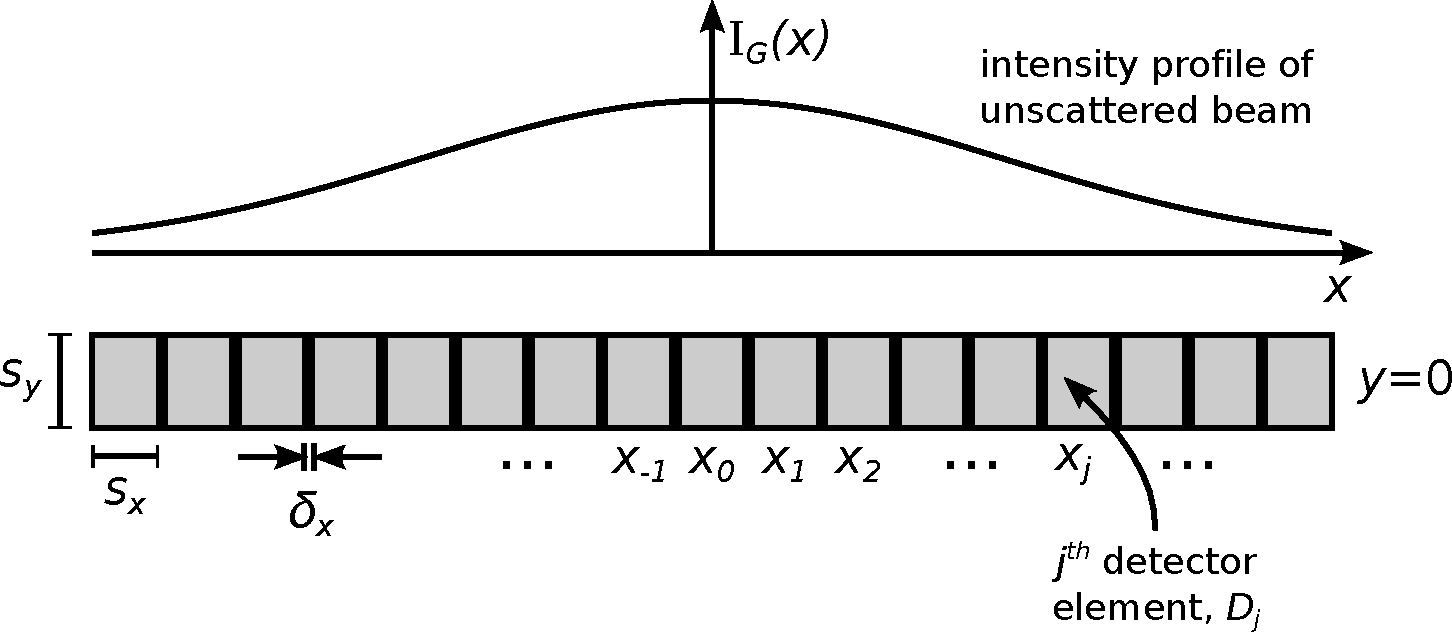
\includegraphics[width = \textwidth]{%
    Chapters/DesignConsiderations/figs/detector_array.pdf}
  \caption[Finite sampling volumes in a detector array]{%
    The probe radiation and the reference beam
    are interfered on a detector array.
    The array consists of numerous detector elements,
    each of size $s_x \times s_y$ and with interelement spacing $\delta_x$.
    The unscattered beam is centered on $x = x_0$ and $y = 0$, and
    its intensity profile varies only weakly over any given element.
    The finite size of each detector element tends to attenuate
    short wavelength components of the incident optical signal.
  }
\label{fig:DesignConsiderations:detector_array}
\end{figure}


\subsection{Finite sampling-volume effects}
\label{sec:DesignConsiderations:geometric:finite_sampling_volume}
Practically speaking, detection is always effected
via detector elements of \emph{finite} size,
with the output of each detector element
corresponding to the incident intensity
\emph{averaged} over the element's active area.
This averaging acts as a low-pass filter in the spatial domain and
is referred to as the finite sampling-volume effect~\cite{bravenec_rsi95}.

Finite sampling-volume effects dictate
a heterodyne interferometer's wavenumber response~\cite{davis_rsi16}.
To see this, assume that measurements
are made with the detector array shown in
Fig.~\ref{fig:DesignConsiderations:detector_array}.
Let the $j$\ts{th} detector element $D_j$ be centered on $x_{\image,j}$
and $y_{\image} = 0$.
Integrating the optical intensity $\tilde{I}_{IQ}(\vect{r}_{\image}, t)$
corresponding to fluctuations in the baseband signal from
(\ref{eq:InterferometricMethods:heterodyne_total_fluctuating_intensity})
over the face of detector element $D_j$ yields
the corresponding optical power
\begin{align}
  \tilde{P}_{IQ,j}(t)
  &=
  \int_{D_j} \tilde{I}_{IQ}(\vect{r}_{\image}, t) dA
  \notag \\
  &\approx
  I_G(\vect{r}_{\image,j}) s_y
  \int_{x_{\image,j} - s_x / 2}^{x_{\image,j} + s_x / 2}
  \tilde{\phi}(x_{\image}, t)
  dx_{\image};
  \label{eq:DesignConsiderations:fluctuating_baseband_equivalent_optical_power_per_element_v1}
\end{align}
here, the intensity profile $I_G(\vect{r}_{\image})$
has been assumed to be approximately constant
over the face of the detector element.
Because (\ref{eq:DesignConsiderations:fluctuating_baseband_equivalent_optical_power_per_element_v1})
is linear in $\tilde{\phi}$,
it is suitable to consider a single Fourier mode
\begin{equation}
  \tilde{\phi}(x_{\image}, t)
  =
  \tilde{\phi}_0 \cos(k_{\image} x_{\image} - \omega t)
\end{equation}
for which (\ref{eq:DesignConsiderations:fluctuating_baseband_equivalent_optical_power_per_element_v1})
reduces to
\begin{equation}
  \tilde{P}_{IQ,j}(t)
  =
  I_G(\vect{r}_{\image,j}) A
  \cdot
  T_{\text{fsv}}(k_{\image})
  \cdot
  \tilde{\phi}_0 \cos(k_{\image} x_{\image} - \omega t),
  \label{eq:DesignConsiderations:fluctuating_baseband_equivalent_optical_power_per_element_v2}
\end{equation}
where $A = s_x s_y$ is the area of the detector element,
\begin{equation}
  T_{\text{fsv}}(k_{\image})
  \equiv
  \sinc\left( \frac{k_{\image}}{k_{\text{fsv},\image}} \right)
  \label{eq:DesignConsiderations:finite_sampling_volume_transfer_function}
\end{equation}
is the finite sampling-volume transfer function,
\begin{equation}
  \sinc(x) = \frac{\sin(\pi x)}{\pi x}
  \label{eq:DesignConsiderations:normalized_sinc}
\end{equation}
is the normalized sinc function, and
\begin{equation}
  k_{\text{fsv},\image} = \frac{2 \pi}{s_x}
  \label{eq:DesignConsiderations:finite_sampling_volume_cutoff_image_plane}
\end{equation}
is the first zero of $T_{\text{fsv}}(k_{\image})$.
Recalling that an object-plane wavenumber $k$
is imaged as $k_{\image} = k / M$
in a magnification-$M$ imaging system,
the corresponding object-plane finite sampling-volume wavenumber cutoff is
\begin{equation}
  k_{\text{fsv}} = \frac{2 \pi M}{s_x}.
  \label{eq:DesignConsiderations:finite_sampling_volume_cutoff}
\end{equation}
Now, as in Section~\ref{sec:InterferometricMethods:interferometry:heterodyne},
select the central intensity of the unscattered beam at the detector to be
$I_G(0) = I_{\text{sat}} / 4$, where
$I_{\text{sat}}$ is the detector's linear saturation intensity,
such that
\begin{equation}
  \frac{\tilde{P}_{IQ,j}(t)}{I_{\text{sat}} A}
  =
  \frac{I_G(\vect{r}_{\image,j})}{I_G(0)}
  \cdot
  T_{\text{het}}(k_{\image})
  \cdot
  \tilde{\phi}_0 \cos(k_{\image} x_{\image} - \omega t),
\end{equation}
where
\begin{equation}
  T_{\text{het}}(k_{\image})
  =
  \frac{1}{4} \cdot T_{\text{fsv}}(k_{\image})
  \label{eq:DesignConsiderations:heterodyne_interferometer_wavenumber_transfer_function}
\end{equation}
is the heterodyne interferometer's wavenumber transfer function.
In the limit $s_x \rightarrow 0$, $T_\text{fsv} \rightarrow 1$ and
the heterodyne interferometer's wavenumber transfer function reduces to
(\ref{eq:InterferometricMethods:heterodyne_interferometer_wavenumber_transfer_function}).
Thus, finite sampling-volume effects
introduce a wavenumber dependence into $T_{\text{het}}$,
as shown in Fig.~\ref{fig:DesignConsiderations:fsv_effects}.
Note that finite sampling-volume effects
introduce similar wavenumber dependencies
into the transfer functions of the homodyne interferometer and PCI.

\begin{figure}
  \centering
  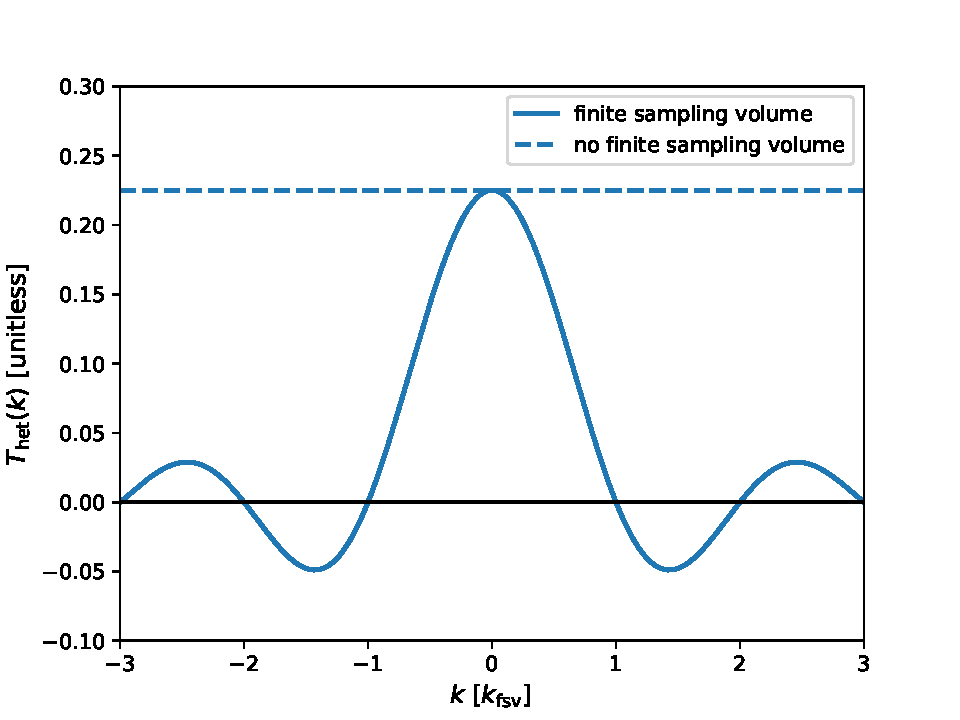
\includegraphics[width = \textwidth]{%
    Chapters/DesignConsiderations/figs/fsv_effects.pdf}
  \caption[Transfer function of heterodyne interferometer with finite sampling-volume effects]{%
    The wavenumber transfer function for a heterodyne interferometer
    with finite sampling-volume effects and
    without finite sampling-volume effects.
  }
\label{fig:DesignConsiderations:fsv_effects}
\end{figure}


\section{Intensity considerations}
\label{sec:DesignConsiderations:intensity}
Ideally, a photovoltaic detector produces an output voltage
\begin{equation}
  V(t) = \mathcal{R}_0 \cdot I(t),
\end{equation}
where $\mathcal{R}_0$ is the detector responsivity and
$I(t)$ is the incident optical intensity.
However, every real-world detector has a saturation intensity $I_{\text{sat}}$
beyond which the output voltage ceases to be a linear function
of the incident optical intensity; that is,
the detector responsivity has an intensity dependence $\mathcal{R}(I)$, and
the detector voltage can be more generally written as
\begin{equation}
  V(t) = \mathcal{R}\left( I(t) \right) \cdot I(t).
\end{equation}
Here, $\mathcal{R}(I)$ is an arbitrary monotonically increasing function
of the incident optical intensity $I$.
Despite the potentially nonlinear response,
the detector voltage remains periodic in $2 \pi / \Delta \omega_0$ and
can be expanded in a Fourier series as
\begin{equation}
  V(t)
  =
  V_0
  +
  \sum_{n = 1}^{\infty}
  V_n \cos\left( n \Delta \omega_0 t + \theta_n \right),
\end{equation}
where $V_n$ and $\theta_n$ are the amplitude and phase, respectively,
of the $n\ts{th}$ harmonic.
Thus, a nonlinear detector response produces
higher-order harmonics in the signal.
In general, $V_n$ and $\theta_n$ can vary in time,
producing sidebands about each harmonic.
Provided the bandwidth of these fluctuations is sufficiently low,
there will be no spectral overlap
between the sidebands of adjacent harmonics, and
bandpass filtering the detector signal about $\Delta \omega_0$ yields
\begin{equation}
  V(t) \approx V_1 \cos[\Delta \omega_0 t + \theta_1(t)]
\end{equation}
with $\theta_1(t) = \phi(t)$, where
$\phi(t)$ is the optical phase shift
between the plasma and reference arms of the interferometer.
However, for fluctuations with sufficiently high bandwidth
(e.g.\ $\omega \sim \Delta\omega_0 / 2$),
the sidebands of adjacent harmonics begin to overlap,
potentially corrupting the phase measurement,
as demonstrated by the example in
Fig.~\ref{fig:DesignConsiderations:nonlinear_heterodyne_detection}.
When operating in the saturated regime,
the heterodyne interferometer's wavenumber transfer function
(\ref{eq:DesignConsiderations:heterodyne_interferometer_wavenumber_transfer_function})
should be multiplied by the prefactor $(V_1 / V_{\text{sat}})$, where
$V_1$ is the amplitude of the heterodyne frequency's fundamental harmonic and
$V_{\text{sat}}$ is the output voltage of the detector
when the incident optical intensity
is equal to the saturation intensity $I_{\text{sat}}$.

\begin{figure}
  \centering
  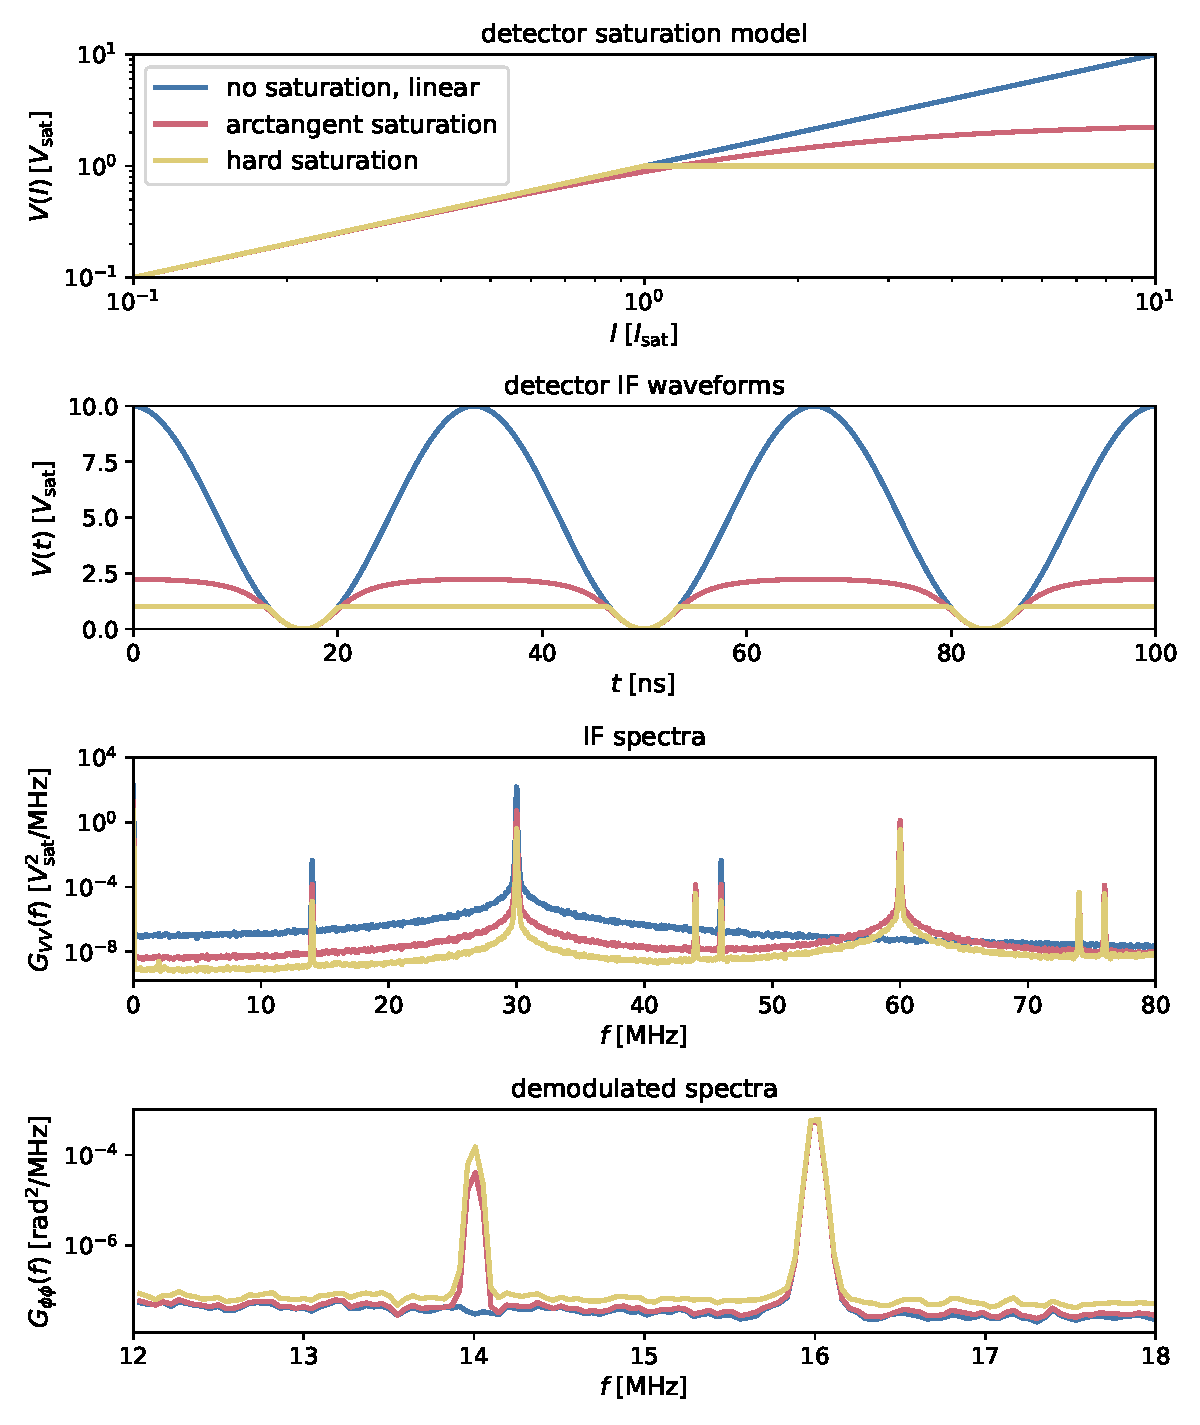
\includegraphics[width = \textwidth]{%
    Chapters/DesignConsiderations/figs/nonlinear_heterodyne_detection.pdf}
  \caption[Heterodyne detection beyond the saturation intensity]{%
    Heterodyne detection beyond the saturation intensity with
    $\Delta\omega_0 = 2\pi \cdot \SI{30}{\mega\hertz}$ and
    $\omega = 2 \pi \cdot \SI{16}{\mega\hertz}$.
    (Top panel): Various detector saturation models.
    The linear model exhibits no saturation,
    the hard saturation model limits the output voltage
    to $V_{\text{sat}}$ when the incident optical intensity
    exceeds $I_{\text{sat}}$, and
    the arctangent saturation model exhibits $\SI{1}{\deci\bel}$ compression
    when the incident optical intensity is $I_{\text{sat}}$.
    (2\ts{nd} panel): The intermediate frequency (IF) waveforms
    corresponding to each saturation model when
    $I_{\text{max}} = 10 \, I_{\text{sat}}$.
    The arctangent and hard saturation models distort the IF waveform,
    producing numerous higher-order harmonics.
    (3\ts{rd} panel): Autospectral densities of the IF waveforms.
    The IF waveforms all exhibit peaks at
    the $\SI{30}{\mega\hertz}$ fundamental and
    its corresponding sidebands at
    $\SI{30}{\mega\hertz} \pm \SI{16}{\mega\hertz}$.
    However, the saturated IF waveforms
    also exhibit peaks at the second harmonic ($\SI{60}{\mega\hertz}$)
    and its corresponding sidebands
    ($\SI{60}{\mega\hertz} \pm \SI{16}{\mega\hertz}$).
    (Bottom panel): Autospectral densities of the demodulated phase.
    Note that the $\SI{16}{\mega\hertz}$ fluctuation is correctly identified
    when demodulating all of the IF waveforms.
    However, the saturated IF waveforms also produce
    a \emph{spurious} $\SI{14}{\mega\hertz}$ fluctuation,
    which is attributable to the overlap of
    the $\SI{30}{\mega\hertz}$ and $\SI{60}{\mega\hertz}$ sidebands.
  }
\label{fig:DesignConsiderations:nonlinear_heterodyne_detection}
\end{figure}


\section{Phase noise: sources \& effects}
\label{sec:DesignConsiderations:phase_noise}
Heterodyne interferometry at $\SI{10.6}{\micro\meter}$ relies on both
an optical oscillator (the laser) and
a radio-frequency oscillator
(usually referred to as the local oscillator (LO)).
These oscillators, like all real-world oscillators, exhibit phase noise.
The spectral properties and implications of oscillator phase noise
are reviewed in Appendix~\ref{app:OscillatorPhaseNoise}.
Below, Section~\ref{sec:DesignConsiderations:phase_noise:laser}
shows that a mismatch between the optical path lengths
of the probe beam and the reference beam
injects the laser's phase noise
into the heterodyne interferometer's measurements, while
Section~\ref{sec:DesignConsiderations:phase_noise:LO}
shows that finite coupling time
in the Doppler-shifting modulator
injects the LO's phase noise
into the heterodyne interferometer's measurements.


\subsection{Unmatched optical path lengths \& laser phase noise}
\label{sec:DesignConsiderations:phase_noise:laser}
The external reference-beam interferometry derivations
in Section~\ref{sec:InterferometricMethods:interferometry}
assumed that the laser's angular frequency was fixed
at its nominal value $\omega_0$.
However, the angular frequency of any \emph{real} laser
will exhibit small fluctuations in time,
much like any other real-world oscillator
\cite[Sec.~1.7]{siegman_lasers}.
The electric field of such a Gaussian beam
is well-described by
\begin{equation}
  E_G(\vect{r}, t)
  =
  E_G(\vect{r})
  e^{-i [\omega_0 t + \phi_{\omega_0}(t)]},
\end{equation}
where $\phi_{\omega_0}(t)$ is a zero-mean, stationary, random process
known as the laser's \emph{phase deviation}
whose temporal variation causes
the laser's instantaneous angular frequency
to wander about its nominal value $\omega_0$.

Now, if the interferometer's probe beam and reference beam
traverse different optical path lengths,
the laser's phase deviation will inject
phase noise into the measured signal.
To see this, assume that the optical path length of the probe beam
exceeds that of the reference arm by $L$.
Then, if the reference beam impinging on the detector at time $t$ is
\begin{equation}
  E_R(\vect{r}_{\image}, t)
  =
  E_G(\vect{r}_{\image})
  e^{-i [
    (\omega_0 + \Delta \omega_0) t
    +
    \phi_{\omega_0}(t)
  ]},
\end{equation}
the corresponding imaged probe radiation is
\begin{equation}
  E_P(\vect{r}_{\image}, t)
  =
  E_G(\vect{r}_{\image})
  e^{-i [\omega_0 (t - \tau) + \phi_{\omega_0}(t - \tau)]}
  e^{i \bar{\phi}}
  \left[%
    1
    +
    i \tilde{\phi}(x_{\image}, t)
  \right],
\end{equation}
where $\tau = L / c$ is the time delay
associated with the optical path-length difference $L$.
Define the corresponding instrumental phase noise as
\begin{equation}
  \delta \phi_{\omega_0}(t, \tau)
  =
  \phi_{\omega_0}(t + \tau)
  -
  \phi_{\omega_0}(t).
\end{equation}
Typically, $\delta \phi_{\omega_0}(t, \tau) \ll 1$.
Then, appropriately generalizing the derivations between
(\ref{eq:InterferometricMethods:heterodyne_intensity}) and
(\ref{eq:InterferometricMethods:heterodyne_total_fluctuating_intensity}),
one readily finds that the total fluctuating power
in the heterodyne interferometer's demodulated signals is
\begin{equation}
  \tilde{I}_{IQ}(\vect{r}_{\image}, t)
  =
  I_G(\vect{r}_{\image})
  \left[%
    \tilde{\phi}(x_{\image}, t)
    +
    \delta \phi_{\omega_0}(t - \tau, \tau)
  \right],
\end{equation}
and the \emph{measured} phase fluctuation
$\tilde{\phi}_m(x_{\image}, t)
=
\tilde{I}_{IQ}(\vect{r}_{\image}, t) / I_G(\vect{r}_{\image})$ is
\begin{equation}
  \tilde{\phi}_m(x_{\image}, t)
  =
  \tilde{\phi}(x_{\image}, t)
  +
  \delta \phi_{\omega_0}(t - \tau, \tau);
  \label{eq:DesignConsiderations:measured_phase_with_laser_jitter}
\end{equation}
that is, the fluctuating signal is contaminated
by the laser's phase noise.
The spectral properties of $\delta \phi_{\omega_0}(t, \tau)$
are thoroughly discussed in Appendix~\ref{app:OscillatorPhaseNoise}.
As $\delta \phi_{\omega_0}(t, \tau)$ and
$\tilde{\phi}(x_{\image}, t)$ are uncorrelated,
the one-sided autospectral density of the measured phase fluctuations is
\begin{equation}
    G_{\tilde{\phi}_m,\tilde{\phi}_m}(f)
    =
    G_{\tilde{\phi},\tilde{\phi}}(f)
    +
    8 \sin^2(\pi f \tau) \mathcal{L}_{\omega_0}(f),
\end{equation}
where
$G_{\tilde{\phi},\tilde{\phi}}(f)$ is the \emph{true}
one-sided autospectral density of the phase fluctuation $\tilde{\phi}$ and
$\mathcal{L}_{\omega_0}(f)$ is the phase noise of the laser,
as defined in Appendix~\ref{app:OscillatorPhaseNoise}.


\subsection{Modulator's finite coupling time \& LO phase noise}
\label{sec:DesignConsiderations:phase_noise:LO}
Heterodyne detection is effected by
modestly Doppler shifting the reference beam
relative to the plasma beam.
It is easy to Doppler shift $\SI{10.6}{\micro\meter}$ radiation
by tens of $MHz$ with a Germanium acousto-optic modulator (AOM).
The operation of a typical AOM is sketched in
Fig.~\ref{fig:DesignConsiderations:aom_scattering_diagram}.
A piezo-actuator drives sound waves
of angular frequency $\Delta \omega_0$
through the Germanium crystal, and
the sound waves act as a diffraction grating
that propagates at the crystal's sound speed $c_s$.
When a beam of vacuum wavelength $\lambda_0$
impinges upon the crystal at the Bragg angle
\begin{equation}
  \theta_B = \frac{\lambda_0 \cdot \Delta \omega_0}{4 \pi c_s},
  \label{eq:DesignConsiderations:Bragg_angle}
\end{equation}
a portion of the beam is deflected and
Doppler shifted by angular frequency $\Delta \omega_0$
\cite[Sec.~20.1]{saleh_and_teich}.
The power in the deflected beam
is controlled by the intensity of the sound waves.

\begin{figure}
  \centering
  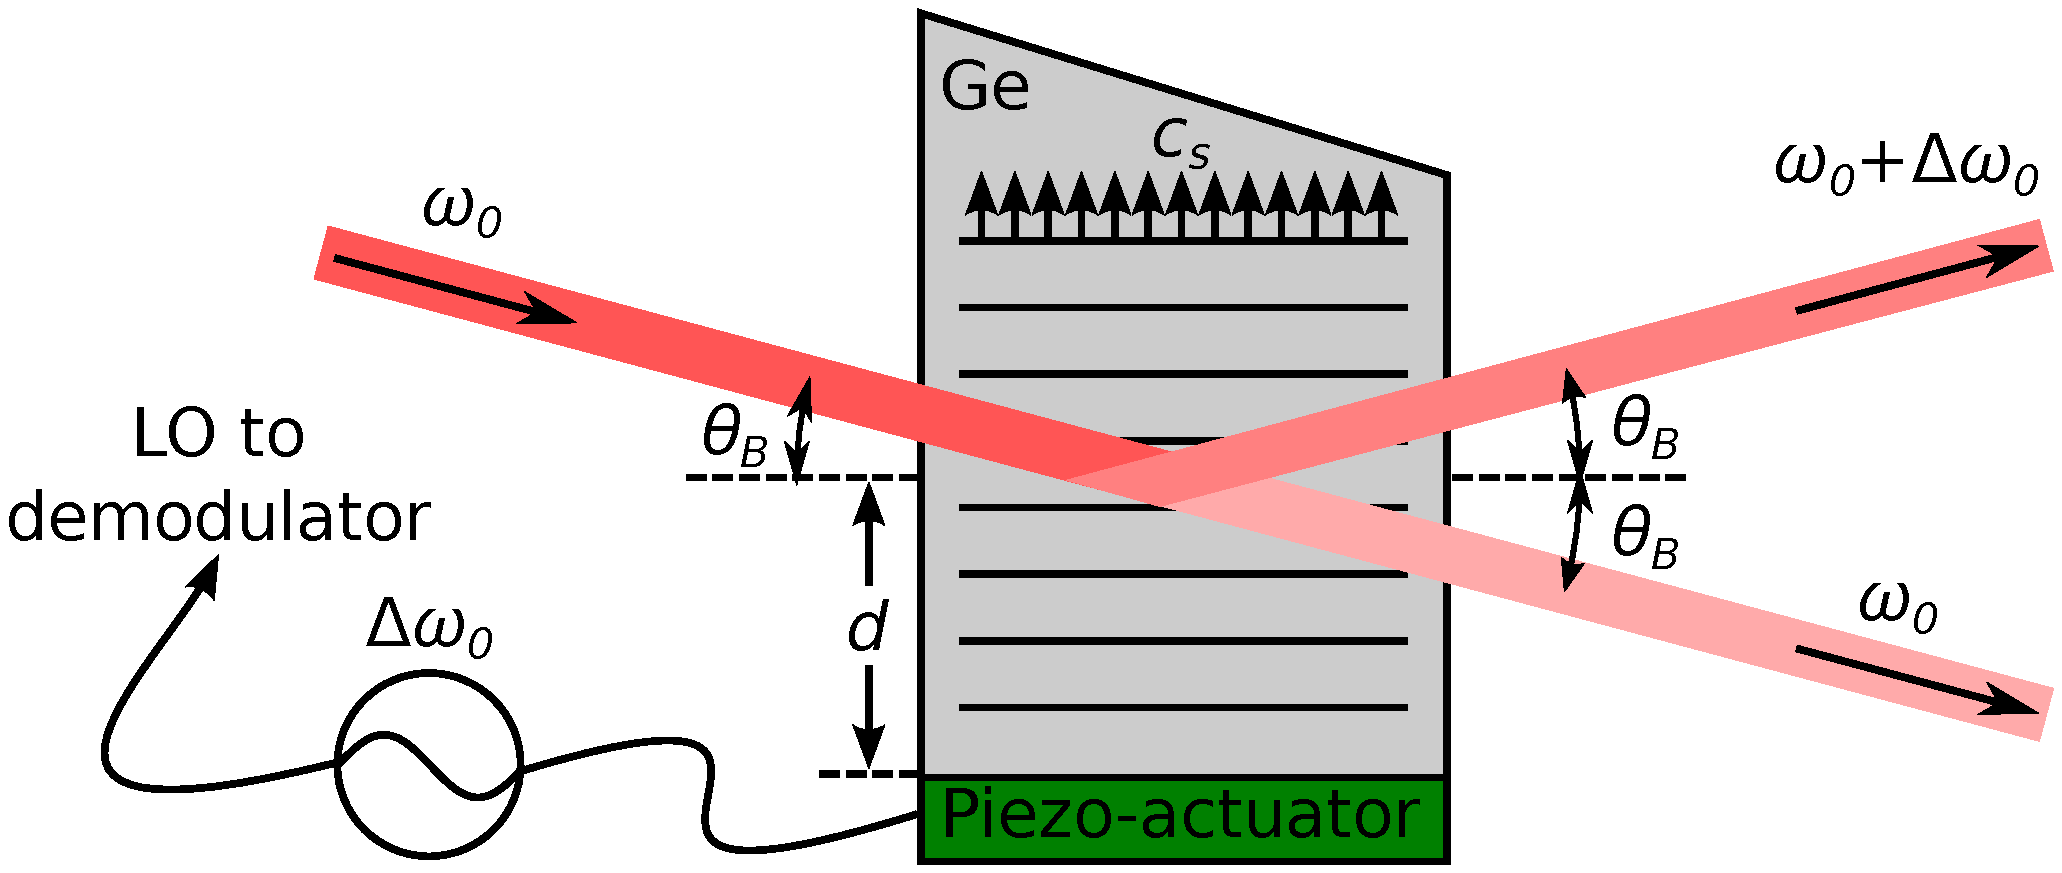
\includegraphics[width = \textwidth]{%
    Chapters/DesignConsiderations/figs/aom_scattering_diagram.pdf}
  \caption[Illustration of AOM operation in a heterodyne interferometer]{%
    An illustration of AOM operation in a heterodyne interferometer.
    A piezo-actuator drives sound waves of angular frequency $\Delta \omega_0$
    through a crystal (usually Germanium for $\SI{10.6}{\micro\meter}$ light),
    and these sound waves deflect and Doppler shift light
    that is incident upon the crystal at the Bragg angle $\theta_B$.
    The sound waves propagate from the piezo-actuator
    to the AOM's optically active region
    over finite time $\tau = d / c_s$.
    The RF waveform that drives the piezo-actuator
    is sampled and used to demodulate the heterodyne interference signal.
    Note that for simplicity the refraction of the beam
    as it enters and exits the crystal is \emph{not} depicted.}
\label{fig:DesignConsiderations:aom_scattering_diagram}
\end{figure}

The coupling of the AOM's drive signal to the deflected beam
occurs on the crystal's sound-wave timescale.
If the sound waves must propagate a distance $d$
from the piezo-actuator to the AOM's optically active region,
the drive signal is coupled to the deflected beam
only after time delay $\tau = d / c_s$.
The sound speed in Germanium is $c_s = \SI{5400}{\meter\per\second}$
such that a distance $d = \SI{1}{\centi\meter}$
is accompanied by a time delay $\tau = \SI{1.85}{\micro\second}$.
Note that this is large compared to many other timescales
typically considered in interferometry;
for example, light propagates
through $\SI{1}{\meter}$ of air
in only $\SI{3.33}{\nano\second}$,
and an RF signal propagates
through $\SI{1}{\meter}$ of RG-58 coaxial cable
(for which the index of refraction is $\sim 3 / 2$)
in only $\SI{5}{\nano\second}$.

In the presence of LO phase noise,
an AOM's finite coupling time
can degrade the performance of a heterodyne interferometer.
A local oscillator with phase noise is well-described by
\begin{equation}
  V_{\text{LO}}(t)
  =
  V_{0}
  e^{-i [\Delta \omega_0 t + \phi_{\Delta \omega_0}(t)]},
\end{equation}
where $\phi_{\Delta \omega_0}(t)$ is a zero-mean, stationary, random process
known as the LO's \emph{phase deviation}
whose temporal variation causes
the LO's instantaneous angular frequency
to wander about its nominal value $\Delta \omega_0$.
Then, to account for the AOM's finite coupling time and
the LO phase noise, take
$\Delta \omega_0 t
\rightarrow
[\Delta \omega_0 (t - \tau) + \phi_{\Delta \omega_0}(t - \tau)]$
in the heterodyne intensity
(\ref{eq:InterferometricMethods:heterodyne_intensity}).
Neglecting finite sampling-volume effects,
the heterodyne output voltage from a given detector element
is simply proportional to the local intensity, i.e.\
\begin{align}
  \begin{aligned}
    V_{\text{het}}(t)
    &=
    2 V_0
    \bigl\{%
      1
      +
      \cos\left[%
        \Delta \omega_0 t
        +
        \bar{\phi}_{\text{eff}}
        +
        \phi_{\Delta \omega_0}(t - \tau)
      \right]
      \\
      &\quad-
      \tilde{\phi}(x_{\image}, t)
      \sin\left[%
        \Delta \omega_0 t
        +
        \bar{\phi}_{\text{eff}}
        +
        \phi_{\Delta \omega_0}(t - \tau)
      \right]
    \bigr\},
  \end{aligned}
\end{align}
where $\bar{\phi}_{\text{eff}} = \bar{\phi} - \Delta \omega_0 \tau$.
Then, taking inspiration from the demodulated optical intensities
(\ref{eq:InterferometricMethods:heterodyne_interferometer_I_and_Q_intensity}),
the demodulated in-phase ($V_I$) and quadrature ($V_Q$) voltages are defined as
\begin{align}
  V_{I}(t)
  +
  i \cdot V_{Q}(t)
  &=
  \frac{1}{V_0}
  \langle
    V_{\text{LO}}(t)
    \cdot
    V_{\text{het}}(t)
  \rangle_{\Delta \omega_0}
  \notag \\
  &=
  V_0
  e^{i \bar{\phi}_{\text{eff}}}
  \left[
    1
    +
    \tilde{\phi}(x_{\image}, t)
    +
    \delta \phi_{\Delta \omega_0}(t, -\tau)
  \right],
  \label{eq:DesignConsiderations:heterodyne_interferometer_I_and_Q_voltage}
\end{align}
where
\begin{equation}
  \delta \phi_{\Delta \omega_0}(t, \tau)
  =
  \phi_{\Delta \omega_0}(t + \tau)
  -
  \phi_{\Delta \omega_0}(t)
\end{equation}
is the instrumental phase noise.
Comparing the demodulated voltages
(\ref{eq:DesignConsiderations:heterodyne_interferometer_I_and_Q_voltage}) to
the demodulated intensities
(\ref{eq:InterferometricMethods:heterodyne_interferometer_I_and_Q_intensity})
indicates that the \emph{measured} phase fluctuation becomes
\begin{equation}
  \tilde{\phi}_m(x_{\image}, t)
  =
  \tilde{\phi}(x_{\image}, t)
  +
  \delta \phi_{\Delta \omega_0}(t, -\tau);
\end{equation}
that is, the fluctuating signal is contaminated
by the LO phase noise.
The spectral properties of $\delta \phi_{\Delta\omega_0}(t, \tau)$
are thoroughly discussed in Appendix~\ref{app:OscillatorPhaseNoise}.
As $\delta \phi_{\omega_0}(t, \tau)$ and
$\tilde{\phi}(x_{\image}, t)$ are uncorrelated,
the one-sided autospectral density of the measured phase fluctuations is
\begin{equation}
    G_{\tilde{\phi}_m,\tilde{\phi}_m}(f)
    =
    S_{\tilde{\phi},\tilde{\phi}}(f)
    +
    8 \sin^2(\pi f \tau) \mathcal{L}_{\Delta\omega_0}(f),
\end{equation}
where
$G_{\tilde{\phi},\tilde{\phi}}(f)$ is the \emph{true}
one-sided autospectral density of the phase fluctuation $\tilde{\phi}$ and
$\mathcal{L}_{\Delta\omega_0}(f)$ is the phase noise of the LO,
as defined in Appendix~\ref{app:OscillatorPhaseNoise}.


\section{Amplitude noise: sources \& effects}
\label{sec:DesignConsiderations:amplitude_noise}
Detector noise and shot noise are typically
the largest contributors to amplitude noise
in the heterodyne interference signal, while
a noisy amplifier can degrade the signal-to-noise ratio.
The demodulation of such amplitude noise
is throughly discussed by Rakhmanov in~\cite{rakhmanov_ao01}.
While Rakhmanov does not explicitly consider quadrature heterodyne detection,
his results can be naturally applied to quadrature heterodyne detection,
as is done below.


\subsection{Detector noise}
Real-world detector operation is associated with intrinsic noise.
This noise results from, among other things,
Johnson thermal noise in the detector and
shot noise in the background radiation flux
\cite{hamamatsu_ir_detectors}.
A detector's noise is often characterized by
its noise-equivalent power ($NEP$):
when the power of the incident optical signal is equal to the $NEP$,
the signal-to-noise ratio is unity.
Consider optical power $\delta P(t)$ that, when incident upon a detector,
produces a signal that
emulates the statistical properties of the detector noise
(e.g.\ $\delta P(t)$ is a real-valued, zero-mean, stationary, random process).
Then, the $NEP$ corresponds to the root mean square (RMS) of $\delta P(t)$,
and
\begin{equation}
  (NEP)^2
  =
  \int_{\Delta f}
  G_{\delta P, \delta P}(f) df,
  \label{eq:DesignConsiderations:NEP_from_spectral_density}
\end{equation}
where $G_{\delta P, \delta P}(f)$ is
the one-sided autospectral density of $\delta P(t)$ and
the integral is performed over the temporal bandwidth $\Delta f$
of the desired measurement.
Note that $G_{\delta P, \delta P}(f)$ depends on both
extensive (e.g.\ element area) and intensive (e.g.\ element material)
properties of the detector.
To more easily compare detectors of different sizes and materials,
the $NEP$ of a given detector is often parameterized as
\begin{equation}
  NEP = \frac{\sqrt{A \cdot \Delta f}}{D^{*}},
  \label{eq:DesignConsiderations:NEP_from_engineering_parameters}
\end{equation}
where $A$ is the effective area of the detector element,
$\Delta f$ is the temporal bandwidth of the desired measurement, and
$D^{*}$ is the detector's specific detectivity~\cite{jones_josa60}.
Note that larger $D^{*}$ corresponds to increased detector sensitivity.
If $G_{\delta P, \delta P}(f)$ is approximately constant
over the bandwidth $\Delta f$, then equating
(\ref{eq:DesignConsiderations:NEP_from_spectral_density})
to the square of
(\ref{eq:DesignConsiderations:NEP_from_engineering_parameters})
yields
\begin{equation}
  G_{\delta P, \delta P}(f)
  =
  \frac{A}{(D^*)^2}.
  \label{eq:DesignConsiderations:NEP_spectral_density}
\end{equation}

It is now shown shown that
signal demodulation pushes detector noise
near the heterodyne angular frequency $\Delta \omega_0$
into the baseband signal.
Taking inspiration from the demodulated optical intensities
(\ref{eq:InterferometricMethods:heterodyne_interferometer_I_and_Q_intensity}),
define the total detector noise in both
the in-phase ($I$) and quadrature ($Q$) signals to be
\begin{align}
  \delta P_{IQ}(t)
  =
  e^{- i \Delta \omega_0 t} \cdot \delta P(t).
  \label{eq:DesignConsiderations:demodulated_NEP_complex}
\end{align}
Here, the demodulated noise has \emph{not} yet been low-pass filtered.
The autocorrelation function of the demodulated noise is
\begin{align}
  R_{\delta P_{IQ},\delta P_{IQ}}(\tau)
  &=
  E\left[\delta P_{IQ}(t) \cdot \delta P_{IQ}^*(t + \tau) \right]
  \notag \\
  &=
  e^{i \Delta \omega_0 \tau} \cdot R_{\delta P, \delta P}(\tau),
\end{align}
where $z^*$ indicates the complex conjugate of $z$ and
$R_{\delta P, \delta P}(\tau)$ is the
autocorrelation function of the detector noise.
The autospectral density of the demodulated noise is then
\begin{align}
  S_{\delta P_{IQ},\delta P_{IQ}}(f)
  &=
  \mathcal{F}\left[ R_{\delta P_{IQ},\delta P_{IQ}}(\tau) \right](f)
  \notag \\
  &=
  \mathcal{F}\left[
    e^{i 2 \pi \Delta f_0 \tau} \cdot R_{\delta P, \delta P}(\tau)
  \right](f)
  \notag \\
  &=
  S_{\delta P, \delta P}(f + \Delta f_0),
\end{align}
where
$\Delta f_0 = \Delta \omega_0 / (2 \pi)$ is the heterodyne frequency and
$S_{\delta P, \delta P}(f)$ is the autospectral density of the detector noise.
The demodulated signals are typically low-pass filtered
such that only the desired information at $|f| \ll \Delta f_0$
survives
\begin{equation}
  \left.
    S_{\delta P_{IQ},\delta P_{IQ}}(f)
  \right|_{|f| \ll \Delta f_0}
  \approx
  S_{\delta P, \delta P}(\Delta f_0).
  \label{eq:DesignConsiderations:detector_noise_demodulated}
\end{equation}
Thus, the detector noise at the heterodyne frequency $\Delta f_0$
is pushed into the baseband signal via the demodulation process.
Note that the autospectral density of the demodulated detector noise
(\ref{eq:DesignConsiderations:detector_noise_demodulated})
is in agreement with the literature
(e.g.\ see Rakhmanov's Eq.~(47) in~\cite{rakhmanov_ao01}
with $d_1 = 1 / 2$ for demodulation against a perfect sinusoid;
whereas Rakhmanov considers only \emph{one} of the demodulated channels,
(\ref{eq:DesignConsiderations:detector_noise_demodulated})
considers both the in-phase and quadrature channels and
is thus twice as large as Rakhmanov's expression).
The corresponding one-sided autospectral density
of the demodulated detector noise is
\begin{align}
  \left.
    G_{\delta P_{IQ},\delta P_{IQ}}(f)
  \right|_{|f| \ll \Delta f_0}
  &\approx
  G_{\delta P, \delta P}(\Delta f_0).
  \notag \\
  &=
  \frac{A}{(D^*)^2},
  \label{eq:DesignConsiderations:demodulated_NEP_spectral_density}
\end{align}
where the last line follows from
(\ref{eq:DesignConsiderations:NEP_spectral_density}) and
the assumption that $D^{*}$ is the specific detectivity
for frequencies $f$ in the neighborhood
of the heterodyne frequency $\Delta f_0$.


\subsection{Shot noise}
The discrete nature of the arriving photons results in shot noise.
Well-modeled as a Poisson process,
the shot noise increases as $N_{\gamma}^{1/2}$, where
$N_{\gamma}$ is the number of incident photons.
Because the incident optical power (and hence the number of incident photons)
in the heterodyne optical signal is modulated as a function of time,
the corresponding shot noise is inherently nonstationary.
Surprisingly, however, the demodulated shot noise \emph{is} stationary
(e.g.\ see Rakhmanov's Eq.~(59) in~\cite{rakhmanov_ao01}).
Note that Rakhmanov only considers \emph{one} of the demodulated signals, and
maximizing the signal-to-noise ratio in the demodulated signal
requires careful selection of the local oscillator's phase
relative to that of the heterodyne signal
(he terms this the ``demodulation phase'' and
represents it via $\gamma$).
However, by employing quadrature heterodyne detection~\cite{carlstrom_rsi88},
in which $\gamma_Q = \gamma_I + \pi / 2$,
the dependence on the demodulation phase vanishes, i.e.\
\begin{align}
  \left.
    S_{\delta P_{IQ}, \delta P_{IQ}}(f)
  \right|_{|f| \ll \Delta f_0}
  &=
  \sum_{j \in \{I, Q\}}
  \left. \left[
    S_{\delta P_j, \delta P_j}(f; \gamma_j)
  \right] \right|_{|f| \ll \Delta f_0}
  \notag \\
  &=
  h f_0 P_0,
\end{align}
where
$\delta P_{IQ}(t)$ is as defined in
(\ref{eq:DesignConsiderations:demodulated_NEP_complex}),
$\delta P_I(t) = \real[\delta P_{IQ}(t)]$,
$\delta P_Q(t) = \imag[\delta P_{IQ}(t)]$,
$h$ is the Planck constant,
$f_0$ is the frequency of the incident photons, and
$P_0$ is the DC optical power impinging upon the detector.
The corresponding one-sided autospectral density is
\begin{align}
  \left.
    G_{\delta P_{IQ}, \delta P_{IQ}}(f)
  \right|_{|f| \ll \Delta f_0}
  =
  2 h f_0 P_0.
  \label{eq:DesignConsiderations:demodulated_shot_noise_spectral_density}
\end{align}
Rakhmanov notes that
(\ref{eq:DesignConsiderations:demodulated_shot_noise_spectral_density})
corresponds to the well-known Schottky formula.


\subsection{Amplifier noise}
The noise \emph{factor} $F$ of an RF amplifier is defined as the ratio of
the signal-to-noise ratio at the device's input ($SNR_{\text{in}}$) to
the signal-to-noise ratio at the device's output ($SNR_{\text{out}}$)
\begin{equation}
  F = \frac{SNR_{\text{in}}}{SNR_{\text{out}}};
\end{equation}
often, the noise factor $F$ is given
in terms of the noise \emph{figure} $NF$
\cite{minicircuits_amplifier_terms_defined}
\begin{equation}
  NF = 10 \log_{10} F.
\end{equation}
If several amplifiers are cascaded,
the total noise factor of the amplifier chain
can be computed using the well-known Friis noise-factor formula.
Note that the noise factor is only defined
in the context of a signal-to-noise ratio, so
it is not possible to write down the corresponding
autospectral density of the amplifier noise in absolute units.


\section{Demodulation}
\label{sec:DesignConsiderations:demodulation}
The heterodyne interferometer's IF signal must be demodulated
in order to recover the baseband phase information.
Demodulation is typically described as an analog process
in which the IF signal is \emph{mixed} with a local oscillator (LO), but
demodulation can also be performed digitally
\cite{vanzeeland_rsi08, mlynek_fst12} or
with non-mixer-based analog electronics~\cite{mlynek_rsi17}.
The focus here, however, is on the analog, mixer-based approach.
Section~\ref{sec:DesignConsiderations:demodulation:ideal}
describes ideal analog demodulation.
Sections~\ref{sec:DesignConsiderations:demodulation:nonideal_mixing} and
\ref{sec:DesignConsiderations:demodulation:demodulator_imbalances}
discuss nonideal aspects of analog mixers and demodulators, and
Section~\ref{sec:DesignConsiderations:demodulation:imperfection_implications}
analyzes the implications of these imperfections
in the context of fluctuation measurements.


\subsection{Ideal demodulation}
\label{sec:DesignConsiderations:demodulation:ideal}
A typical analog $I\&Q$ demodulator consists of
a $90^{\circ}$ splitter,
two double-balanced mixers, and
a $0^{\circ}$ splitter~\cite{minicircuits_modulators}, as shown in
Fig.~\ref{fig:DesignConsiderations:analog_IQ_demodulator}(a).
The $90^{\circ}$ splitter divides the incident local oscillator (LO) signal
\begin{equation}
  \text{LO}(t) = 2 \cos(\Delta\omega_0 t)
\end{equation}
into an ``in-phase'' copy of the LO
\begin{equation}
  \text{LO}_0(t)
  =
  \sqrt{2} \cos(\Delta\omega_0 t)
\end{equation}
and a $\pi / 2$ phase-advanced copy of the LO
\begin{equation}
  \text{LO}_{\pi / 2}(t)
  =
  \sqrt{2} \cos\left( \Delta\omega_0 t + \frac{\pi}{2} \right)
  =
  -\sqrt{2} \sin(\Delta\omega_0 t).
\end{equation}
Note that the power (i.e.\ the mean-square value) in the incident LO signal
is split evenly between $\text{LO}_0(t)$ and $\text{LO}_{\pi / 2}(t)$.
Further, the normalization of $\text{LO}(t)$ has been specified such that
the power in both $\text{LO}_0(t)$ and $\text{LO}_{\pi / 2}(t)$ is unity,
which simplifies the below discussion of power flow through the demodulator.
The $0^{\circ}$ splitter divides the intermediate frequency (IF) signal
\begin{equation}
  \text{IF}(t) = A_{\text{IF}} \cos(\Delta\omega_0 t + \phi)
  \label{eq:DesignConsiderations:IF_perfect_sinusoid}
\end{equation}
into two identical copies of the IF
\begin{equation}
  \text{IF}_0(t)
  =
  \frac{A_{\text{IF}}}{\sqrt{2}} \cos(\Delta\omega_0 t + \phi).
\end{equation}
Like the LO signal, the power in the incident IF signal
is split evenly between the two copies.
The signal at the demodulator's in-phase ($I$) port
then corresponds to the product of
$\text{IF}_0(t)$ with the in-phase LO signal $\text{LO}_0(t)$:
\begin{equation}
  \text{LO}_0(t) \cdot \text{IF}_0(t)
  =
  \frac{A_{\text{IF}}}{2}
  \left[
    \cos(\phi) + \cos(2 \Delta\omega_0 t + \phi)
  \right].
\end{equation}
Such signal multiplication is often referred to as ``mixing''.
Low-pass filtering the signal exiting the demodulator's $I$ port
yields the baseband in-phase signal
\begin{equation}
  I = \frac{A_{\text{IF}}}{2} \cos\phi.
\end{equation}
Similar reasoning regarding the product
$\text{LO}_{\pi / 2}(t) \cdot \text{IF}_0(t)$
at the demodulator's quadrature ($Q$) port
yields the baseband quadrature signal
\begin{equation}
  Q = \frac{A_{\text{IF}}}{2} \sin\phi.
\end{equation}
Note that the total power $I^2 + Q^2$ in the $I\&Q$ signals
is $\SI{3}{\decibel}$ lower
than the power in the incident IF signal.
This is known as the \emph{conversion loss} of the demodulator, and
it results from low-pass filtering the $I\&Q$ signals;
real-world demodulators will have larger conversion losses
due to the additional effects of dissipation and other nonideal effects.
An \emph{absolute} phase measurement $\phi_m$ is then obtained via
\begin{equation}
  \phi_m = \atan\left( \frac{Q}{I} \right),
  \label{eq:DesignConsiderations:phase_from_arctangent}
\end{equation}
independent of the power in the incident IF signal.
Note that in the ideal case the measured phase is
equal to the true phase, i.e.\ $\phi_m = \phi$.

\begin{figure}
  \centering
  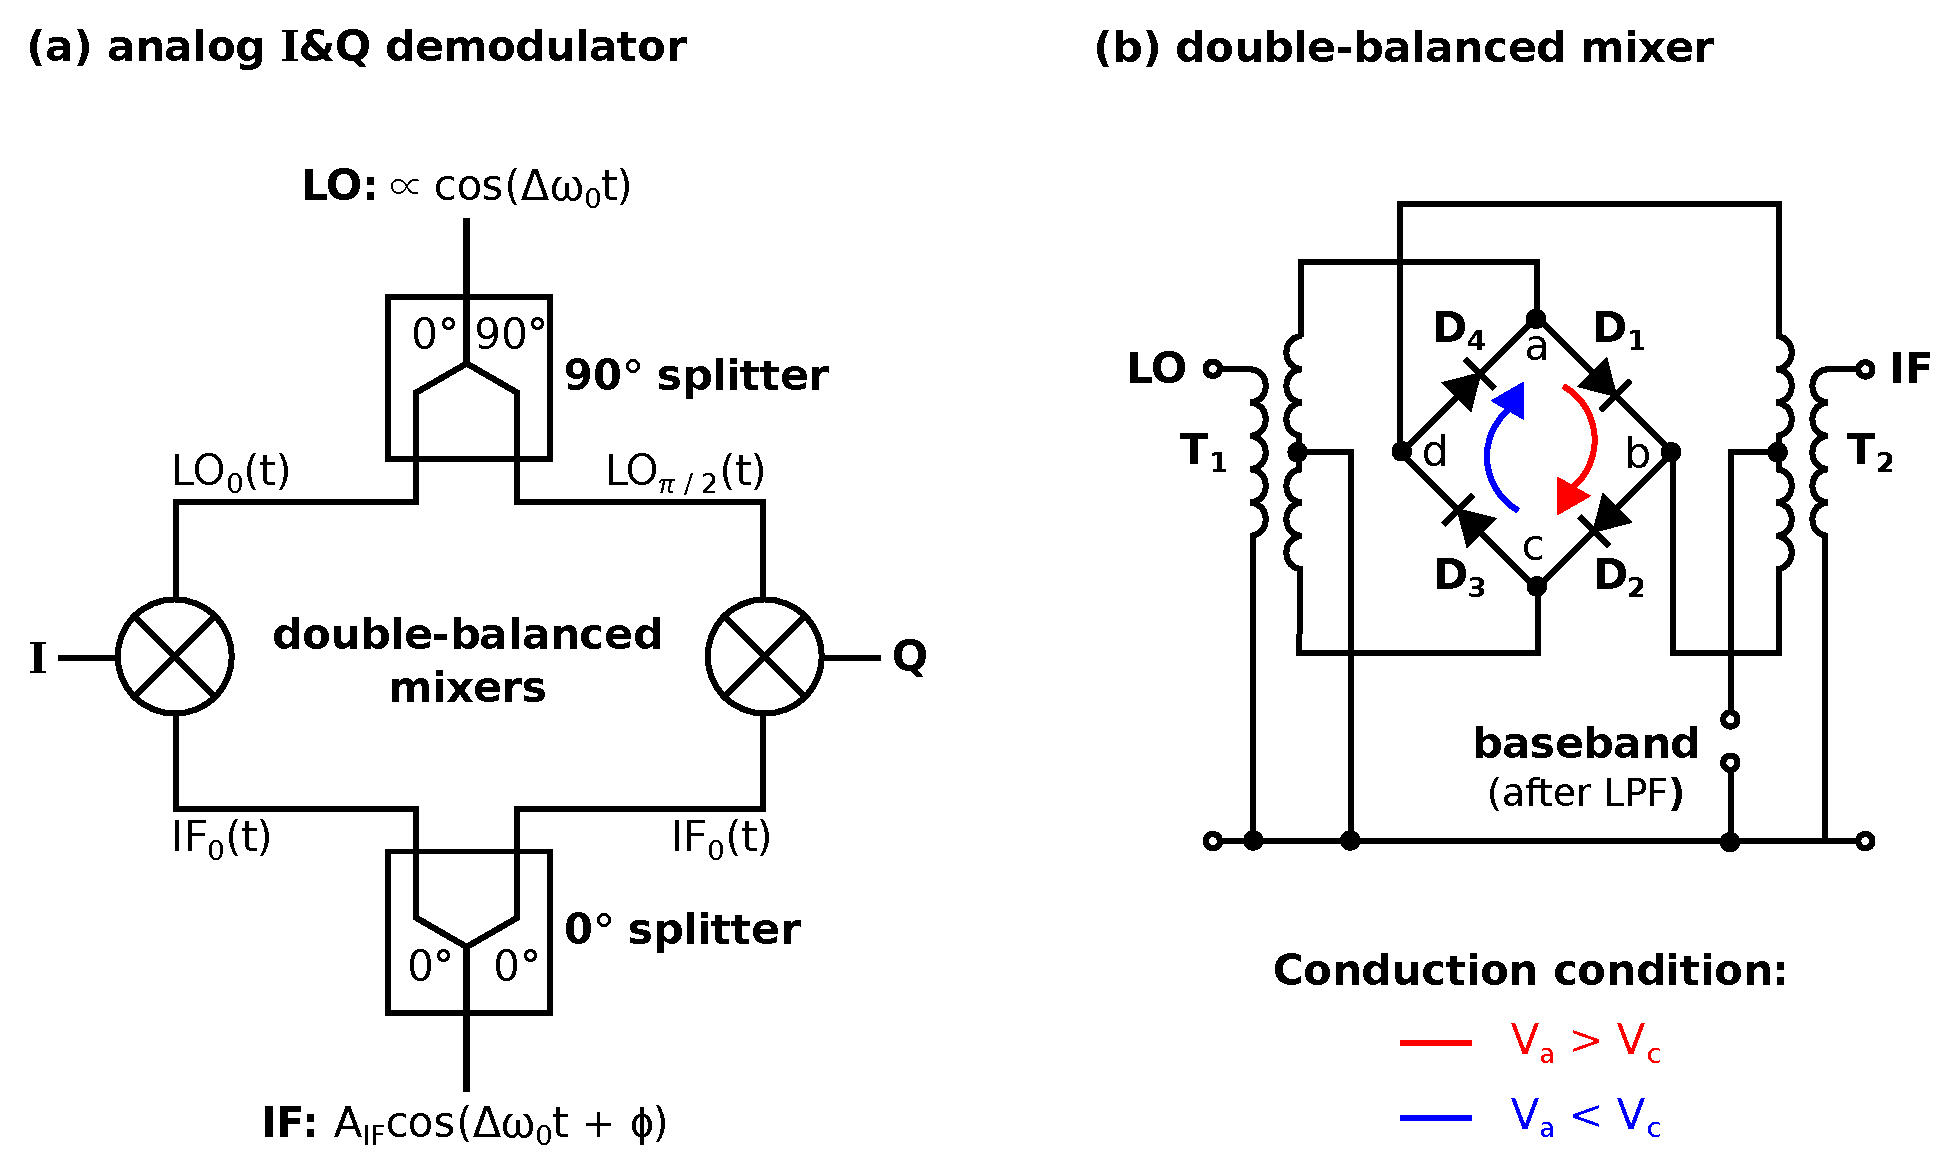
\includegraphics[width = \textwidth]{%
    Chapters/DesignConsiderations/figs/analog_IQ_demodulator.pdf}
  \caption[Components of a typical analog $I\&Q$ demodulator]{%
    (a) A typical analog $I\&Q$ demodulator and
    (b) a typical diode-ring double-balanced mixer.}
  \label{fig:DesignConsiderations:analog_IQ_demodulator}
\end{figure}


\subsection{Nonideal mixing}
\label{sec:DesignConsiderations:demodulation:nonideal_mixing}
In Section~\ref{sec:DesignConsiderations:demodulation:ideal},
mixing was idealized as the multiplication of the IF signal by the LO signal.
However, in practice, more complex process are used
to maximize the mixer's linear dynamic range and minimize its noise figure
\cite{analog_devices_mix_and_mod,bryant_mult_vs_mod}.

For example, a typical ring-diode double-balanced mixer
is shown in Fig.~\ref{fig:DesignConsiderations:analog_IQ_demodulator}(b).
The balun transformers $T_1$ and $T_2$
isolate the baseband port from the LO and IF ports.
Typically, the LO power is $\sim \SI{20}{\deci\bel}$ larger than the IF power.
As a result, the LO alone is responsible
for biasing the mixer's diodes into conduction.
Note that the diodes are not all simultaneously biased into conduction.
Instead, when $V_a > V_c$ (neglecting the diode drops),
diodes $D_1$ and $D_2$ are forced into conduction such that
$V_b$ acts as a virtual ground for the IF signal
coupled through transformer $T_2$.
Then, when the LO changes sign such that $V_a < V_c$,
diodes $D_1$ and $D_2$ stop conducting, and
diodes $D_3$ and $D_4$ begin to conduct,
forcing the virtual ground to jump from $V_b$ to $V_d$.
Thus, the ring diode acts as a switch
for the polarization of the coupled IF signal,
with the switching governed by the sign and frequency of the LO.
Low-pass filtering the polarization-modulated IF, of course,
yields the desired baseband signal.
Note that the diode switching time should be minimized
for optimal modulation,
explaining why some manufacturers
advocate the use of a square, rather than a sinusoidal, LO
\cite{minicircuits_mixer_faqs}.

This polarization modulation can alter the baseband spectrum.
To see this, note that the sign of the in-phase LO signal
is simply a zero-mean square wave with even symmetry about the origin,
as shown in the lower pane of
Fig.~\ref{fig:DesignConsiderations:LO_switching_function}.
The Fourier series of such a square wave
consists of a sum over all of the LO's \emph{odd} harmonics:
\begin{align}
  \text{sgn}\left( \text{LO}_0(t) \right)
  &=
  \frac{4}{\pi}
  \sum_{n = 1}^{\infty}
  \frac{(-1)^{n - 1}}{2n - 1} \cos[(2n - 1) \Delta\omega_0 t]
  \\
  &\begin{aligned}
    =
    \frac{4}{\pi}
    \biggl[%
      \cos(\Delta\omega_0 t)
      &-
      \frac{1}{3} \cos(3 \Delta\omega_0 t)
      +
      \cdots
    \biggr].
  \end{aligned}
  \notag
\end{align}
Now, if the IF signal is a perfect sinusoid
as in (\ref{eq:DesignConsiderations:IF_perfect_sinusoid}),
following Section~\ref{sec:DesignConsiderations:demodulation:ideal}'s program
of mixing the LO with the IF and low-pass filtering yields
the desired in-phase baseband signal, e.g.\
\begin{align}
  I
  &=
  \bigl[%
    \text{sgn}\left( \text{LO}_0(t) \right)
    \cdot
    \text{IF}_0(t)
  \bigr]
  \biggr|_{|\omega| \ll \Delta\omega_0}
  \notag \\
  &=
  \frac{\sqrt{2} A_{\text{IF}}}{\pi} \cos\phi
\end{align}
However, if the path from the mixer's IF port to its baseband port
is not wholly linear
(and every real-world device exhibits \emph{some} degree of nonlinearity),
the IF signal contain contributions from its higher-order harmonics.
If this nonlinearity depends only on the magnitude of the IF
(for example, double-sided saturation or clipping of the signal),
only the odd harmonics of the fundamental will contribute, i.e.\
\begin{equation}
  \text{IF}_0(t)
  =
  \sum_{n = 1}^{\infty}
  A_{2n - 1} \cos\left[ (2n - 1) (\Delta\omega_0 t + \phi) \right],
\end{equation}
where $A_n$ is the Fourier coefficient of the $n\ts{th}$ harmonic.
Typically, $A_n$ decreases as $n$ increases, but
raising the IF amplitude drives more nonlinear interactions and
increases the power in the higher order harmonics relative to the fundamental.
Then,
following Section~\ref{sec:DesignConsiderations:demodulation:ideal}'s program
of mixing the LO with the IF and low-pass filtering yields
\begin{align}
  I
  &=
  \bigl[%
    \text{sgn}\left( \text{LO}_0(t) \right)
    \cdot
    \text{IF}_0(t)
  \bigr]
  \biggr|_{|\omega| \ll \Delta\omega_0}
  \notag \\
  &=
  \frac{2 A_1}{\pi}
  \left[%
    \cos\phi
    -
    \frac{1}{3}\left( \frac{A_3}{A_1} \right) \cos 3 \phi
    +
    \cdots
  \right].
\end{align}
That is, the higher order harmonics of the IF signal
\emph{beat} with the corresponding higher order harmonics
of the LO switching function
to produce harmonics in the baseband signal.
The coefficient $A_n / (n \cdot A_1)$ gives
the \emph{suppression} of the $n\ts{th}$ harmonic, and
it is typically expressed in decibels
referenced to the power of the carrier, or dBc, as
\begin{equation}
  \text{suppression of $n\ts{th}$ harmonic [dBc]}
  =
  20 \log_{10} \left( \frac{A_n}{n \cdot A_1} \right).
\end{equation}
Noting that $\text{sgn}(\text{LO}_{\pi / 2}(t))$
is an inverted, zero-mean square wave
with \emph{odd} symmetry about the origin,
as shown in the lower pane of
Fig.~\ref{fig:DesignConsiderations:LO_switching_function},
a similar path of reasoning to that used above
shows that the quadrature baseband signal is
\begin{align}
  Q
  &=
  \bigl[%
    \text{sgn}\left( \text{LO}_{\pi / 2}(t) \right)
    \cdot
    \text{IF}_0(t)
  \bigr]
  \biggr|_{\omega \ll \Delta\omega_0}
  \notag \\
  &=
  \frac{2 A_1}{\pi}
  \left[%
    \sin\phi
    +
    \frac{1}{3}\left( \frac{A_3}{A_1} \right) \sin 3 \phi
    +
    \cdots
  \right].
\end{align}
Additional distortion of the baseband signal results
if the IF power becomes comparable the LO power,
say within $\SI{10}{\deci\bel}$,
as the IF signal begins to contribute
to the modulation of the diode conduction.

\begin{figure}
  \centering
  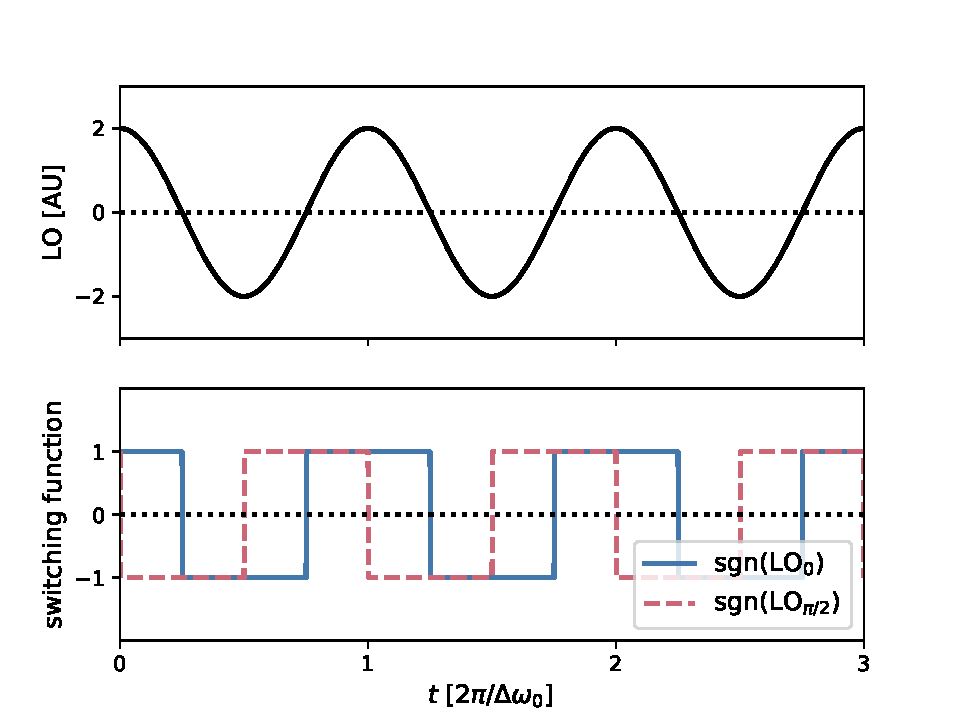
\includegraphics[width = \textwidth]{%
    Chapters/DesignConsiderations/figs/LO_switching_function.pdf}
  \caption[LO switching functions]{%
    The LO switching functions.
    The top panel displays the incident sinusoidal LO signal, while
    the bottom panel shows the \emph{sign} of
    the in-phase ($\text{LO}_0$) and
    the $\pi / 2$ phase-advanced ($\text{LO}_{\pi / 2}$)
    copies of the LO signals.}
  \label{fig:DesignConsiderations:LO_switching_function}
\end{figure}

Finally, the diodes of the mixers should be matched as closely as possible.
If, for example, diodes $D_1$ and $D_2$
have slightly different voltage drops than diodes $D_3$ and $D_4$,
the virtual grounds at $V_b$ and $V_d$ are not equivalent
when referenced to ground, and
a resulting baseband signal will have a DC offset.
With precision fabrication, however,
it is not uncommon for the DC offset to be smaller than $1\%$
of the amplitude of the baseband fundamental harmonic.


\subsection{Demodulator imbalances}
\label{sec:DesignConsiderations:demodulation:demodulator_imbalances}
In addition to two double-balanced mixers,
an analog $I\&Q$ demodulator also relies on
a $90^{\circ}$ splitter and a $0^{\circ}$ splitter.
Imbalances between any of these components
can result in imbalances in the baseband $I\&Q$ signals.
For example, unequal power division in the splitters
produces amplitude imbalances in the baseband $I\&Q$ signals, while
deviations from the nominal splitter phasings
produces phase imbalances in the baseband $I\&Q$ signals.
As discussed in
Section~\ref{sec:DesignConsiderations:demodulation:nonideal_mixing},
each double-balanced mixer can produce
spectral distortion and DC offsets in the baseband signal;
in addition, differences between the two mixers
can exacerbate amplitude and phase imbalances
in the baseband $I\&Q$ signals.
Taken all together, then,
the most general form for the baseband $I\&Q$ signals is
\begin{align}
  I
  &=
  I_1 \left\{%
    \cos\phi
    -
    \frac{I_3}{3 I_1}
    \cos \left( 3 \phi \right)
    +
    \cdots
  \right\}
  +
  \delta I,
  \label{eq:DesignConsiderations:I_general}
  \\
  Q
  &=
  Q_1 \left\{%
    \sin \left( \phi + \delta \right)
    +
    \frac{Q_3}{3 Q_1}
    \sin \left[ 3 \left( \phi + \delta \right) \right]
    +
    \cdots
  \right\}
  +
  \delta Q,
  \label{eq:DesignConsiderations:Q_general}
\end{align}
where
$I_1$ is the amplitude of the in-phase signal's fundamental harmonic,
$I_3$ is the amplitude of the in-phase signal's third harmonic, and
$\delta I$ is the in-phase signal's DC offset.
Similar nomenclature applies to the quadrature signal.
The phase imbalance of the demodulator is $\delta$.
Amplitude imbalances occur when $I_1 \neq Q_1$.
The harmonic suppressions are typically comparable,
e.g.\ $|I_3 / I_1| \approx |Q_3 / Q_1|$.
Note that (\ref{eq:DesignConsiderations:I_general}) and
(\ref{eq:DesignConsiderations:Q_general})
generalize previous forms for the $I\&Q$ signals
\cite{vanzeeland_rsi04}.


\subsection{Effects of demodulator imperfections}
\label{sec:DesignConsiderations:demodulation:imperfection_implications}
Demodulator imperfections produce systematic errors
in the measured phase~\cite{vanzeeland_rsi04,kasten_masters}.
Specifically, if the $I\&Q$ signals suffer from imbalances and nonlinearities,
as shown in (\ref{eq:DesignConsiderations:I_general}) and
(\ref{eq:DesignConsiderations:Q_general}),
then the measured phase $\phi_m$ computed via the inverse tangent formula
(\ref{eq:DesignConsiderations:phase_from_arctangent})
will \emph{not} correspond to the true phase $\phi$, e.g.\
\begin{equation}
  \phi_m = \phi + \delta \phi,
\end{equation}
where $\delta\phi$ is the error in the measured phase.
The phase error is a complicated, periodic function of the true phase,
i.e.\ $\delta\phi = \delta\phi(\phi)$~\cite{vanzeeland_rsi04}.
For small phase fluctuations $|\tilde{\phi}| \ll 1$
about an equilibrium phase $\bar{\phi}$,
the error $\delta\tilde{\phi}$ in the measured fluctuating phase
is simply the \emph{change} in the total phase error
between $\bar{\phi}$ and $\bar{\phi} + \tilde{\phi}$
\cite{kasten_masters}:
\begin{equation}
  \delta\tilde{\phi}
  =
  \delta\phi(\bar{\phi} + \tilde{\phi}) - \delta\phi(\bar{\phi})
  \approx
  \left[%
    \left. \frac{d(\delta\phi)}{d\phi} \right|_{\bar{\phi}}
  \right] \tilde{\phi}.
\end{equation}
Thus, the \emph{relative} error in the measured fluctuating phase is
\begin{equation}
  \frac{\delta\tilde{\phi}}{\tilde{\phi}}
  =
  \left. \frac{d(\delta\phi)}{d\phi} \right|_{\bar{\phi}}
  \label{eq:DesignConsiderations:relative_fluctuation_error}
\end{equation}
The $I\&Q$ Lissajous curves and
the relative errors in the measured fluctuating phase
that result from various demodulator imperfections
are displayed in
Fig.~\ref{fig:DesignConsiderations:effects_of_demodulator_imperfections}.
Obviously, each demodulator imperfection should be minimized
in order to minimize the relative error
in the measured fluctuating phase.

\begin{figure}
  \centering
  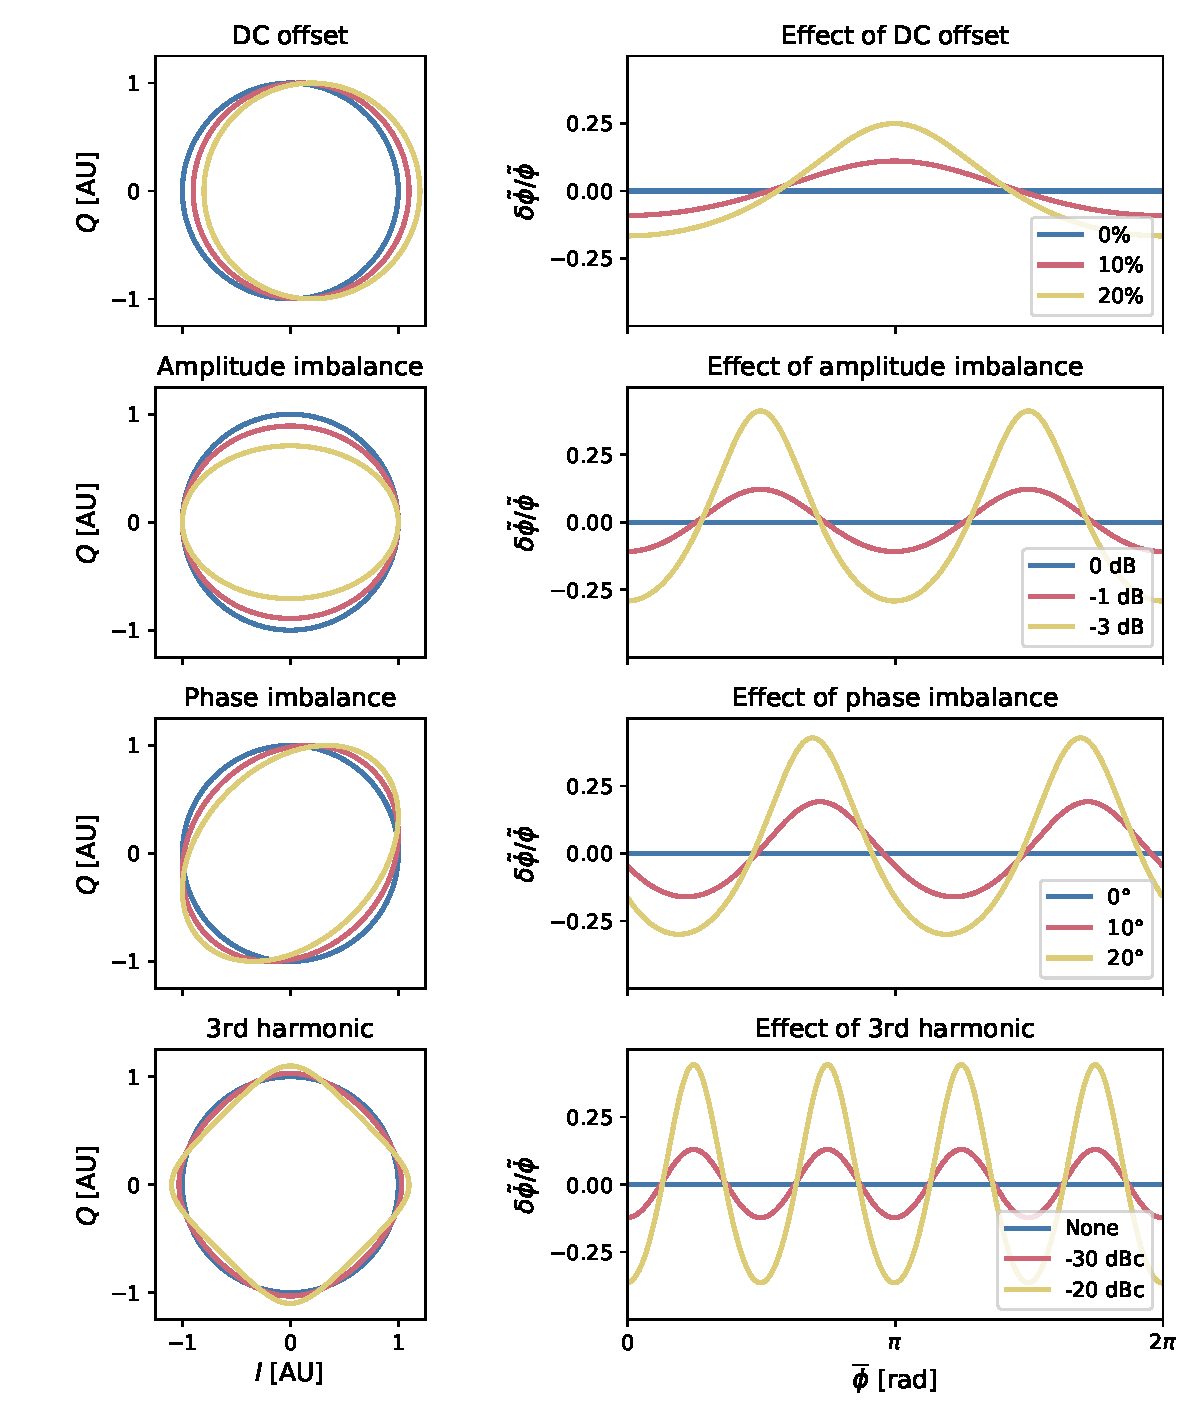
\includegraphics[width = \textwidth]{%
    Chapters/DesignConsiderations/figs/demodulator_imperfections.pdf}
  \caption[Effects of demodulator imperfections]{%
    Demodulator imperfections produce errors in the measured phase.
    The left column displays the Lissajous curves
    that result from plotting
    the quadrature $Q$ vs.\ in-phase $I$ signals, while
    the right column plots the relative error
    $\delta\tilde{\phi} / \tilde{\phi}$
    in the measured fluctuating phase
    as a function of the equilibrium phase $\bar{\phi}$.
    Each row examines a different demodulator imperfection.
  }
  \label{fig:DesignConsiderations:effects_of_demodulator_imperfections}
\end{figure}


\section{Quantization noise}
\label{sec:DesignConsiderations:quantization}
Efficient conversion of an analog signal to a digital record requires
quantization of the signal magnitude and
temporal sampling of these quantized magnitudes~\cite{bennett_bstj48}.
This analog-to-digital conversion
is performed by an instrument known as a digitizer.
If a digitizer has bit depth $N_b$ and
an input-voltage dynamic range $V_{\text{dyn}}$,
then its quantum of voltage $\Delta V$ is
\begin{equation}
  \Delta V
  =
  \frac{V_{\text{dyn}}}{2^{N_b} - 1}
  \approx
  \frac{V_{\text{dyn}}}{2^{N_b}},
  \label{eq:DesignConsiderations:digitizer_voltage_quantum}
\end{equation}
where the approximation is well-satisfied
for typical digitizer bit depths.
At each sampling time,
the analog signal's magnitude is approximated
by the closest quantized value, whose
separation from the true, analog value
will be less than or equal to $\Delta V / 2$.

In general, then, the quantized signal
will differ from the analog signal.
This error $\epsilon$ is known as quantization noise.
The mean square error (i.e.\ variance) attributable to quantization is simply
\begin{equation}
  \overline{\epsilon^2} = \frac{(\Delta V)^2}{12},
  \label{eq:DesignConsiderations:quantization_noise_variance}
\end{equation}
where $\Delta V$ is the digitizer's quantum of voltage,
as given by (\ref{eq:DesignConsiderations:digitizer_voltage_quantum})
\cite{bennett_bstj48}
\cite[Sec.~10.2.4]{bendat_and_piersol}.
For a uniformly sampled record with sampling rate $f_s$,
sufficiently fine quantization $\Delta V$
ensures that the quantization noise is \emph{white}
\cite[Th.~1]{bennett_bstj48}
\cite[Ch.~20]{widrow_and_kollar};
that is, the autospectral density of the quantization noise is
\begin{align}
  S_{\epsilon,\epsilon}(f)
  =
  \frac{\overline{\epsilon^2}}{f_s}
  =
  \frac{(\Delta V)^2}{12 f_s},
  \qquad
  -f_s < f \leq f_s.
  \label{eq:DesignConsiderations:quantization_noise_autospectral_density}
\end{align}
In practice, however, aperture error, jitter, and nonlinearities
may reduce the effective bit depth by one or two bits
\cite[Sec.~10.2.4]{bendat_and_piersol},
increasing the realized quantization noise
relative to that expected from
(\ref{eq:DesignConsiderations:quantization_noise_variance}) and
(\ref{eq:DesignConsiderations:quantization_noise_autospectral_density}).

Quantization noise can be significant
when attempting to measure absolute phase fluctuations
with a heterodyne interferometer.
Recall from the discussion of heterodyne interferometric detection in
Section~\ref{sec:InterferometricMethods:interferometry:heterodyne}
that measurement of the \emph{absolute} phase
requires capturing the full dynamics
of the large, slowly varying equilibrium phase $\bar{\phi}$
in addition to measurement of the fluctuating phase $\tilde{\phi}$.
Because $\tilde{\phi} \ll \bar{\phi}$ in typical situations,
the fluctuations only occupy a small portion
of the digitizer's dynamic range; that is,
fluctuations effectively see a bit depth that
is substantially smaller than the digitizer's nominal bit depth.
Thus, to minimize the effect of quantization noise,
it is absolutely imperative
to utilize the full dynamic range of the digitizer.


\bibliographystyle{plainurl}
\bibliography{references}
%
\chapter{Implementation of a combined PCI-interferometer on \diiid}
\label{ch:Implementation}


\section{Optical-diagnostic access on \diiid}
\label{sec:Implementation:d3d_ports}
\diiid \space provides optical access to its plasmas
through a number of ports, as indicated in
Fig.~\ref{fig:Implementation:d3d_port_locations}.
The ports are labeled according to their
toroidal positions and their sightlines, and
an experimentalist should have at least
a rough familiarity with these conventions.
The toroidal location of a port
is given in degrees clockwise from ``machine north''
when viewing the machine from above
(note that machine north does \emph{not} correspond
to geographic or magnetic north).
The angular separation of adjacent toroidal ports is $15^{\circ}$.
Port sightlines can be vertical or radial.
Ports with vertical (V) sightlines
are labeled sequentially in terms of increasing major radius,
with $V1$ having the smallest major radius and
$V3$ having the largest major radius.
Radial ports (R) have sightlines
that are roughly aligned with the plasma's minor radius, and
they are labeled according to their positions
relative to the plasma midplane:
R0 sits at the plasma midplane,
R+1 and R+2 are the first and second ports
\emph{above} the plasma midplane, respectively, and
R-1 and R-2 are the first and second ports
\emph{below} the plasma midplane, respectively.

\begin{figure}
  \centering
  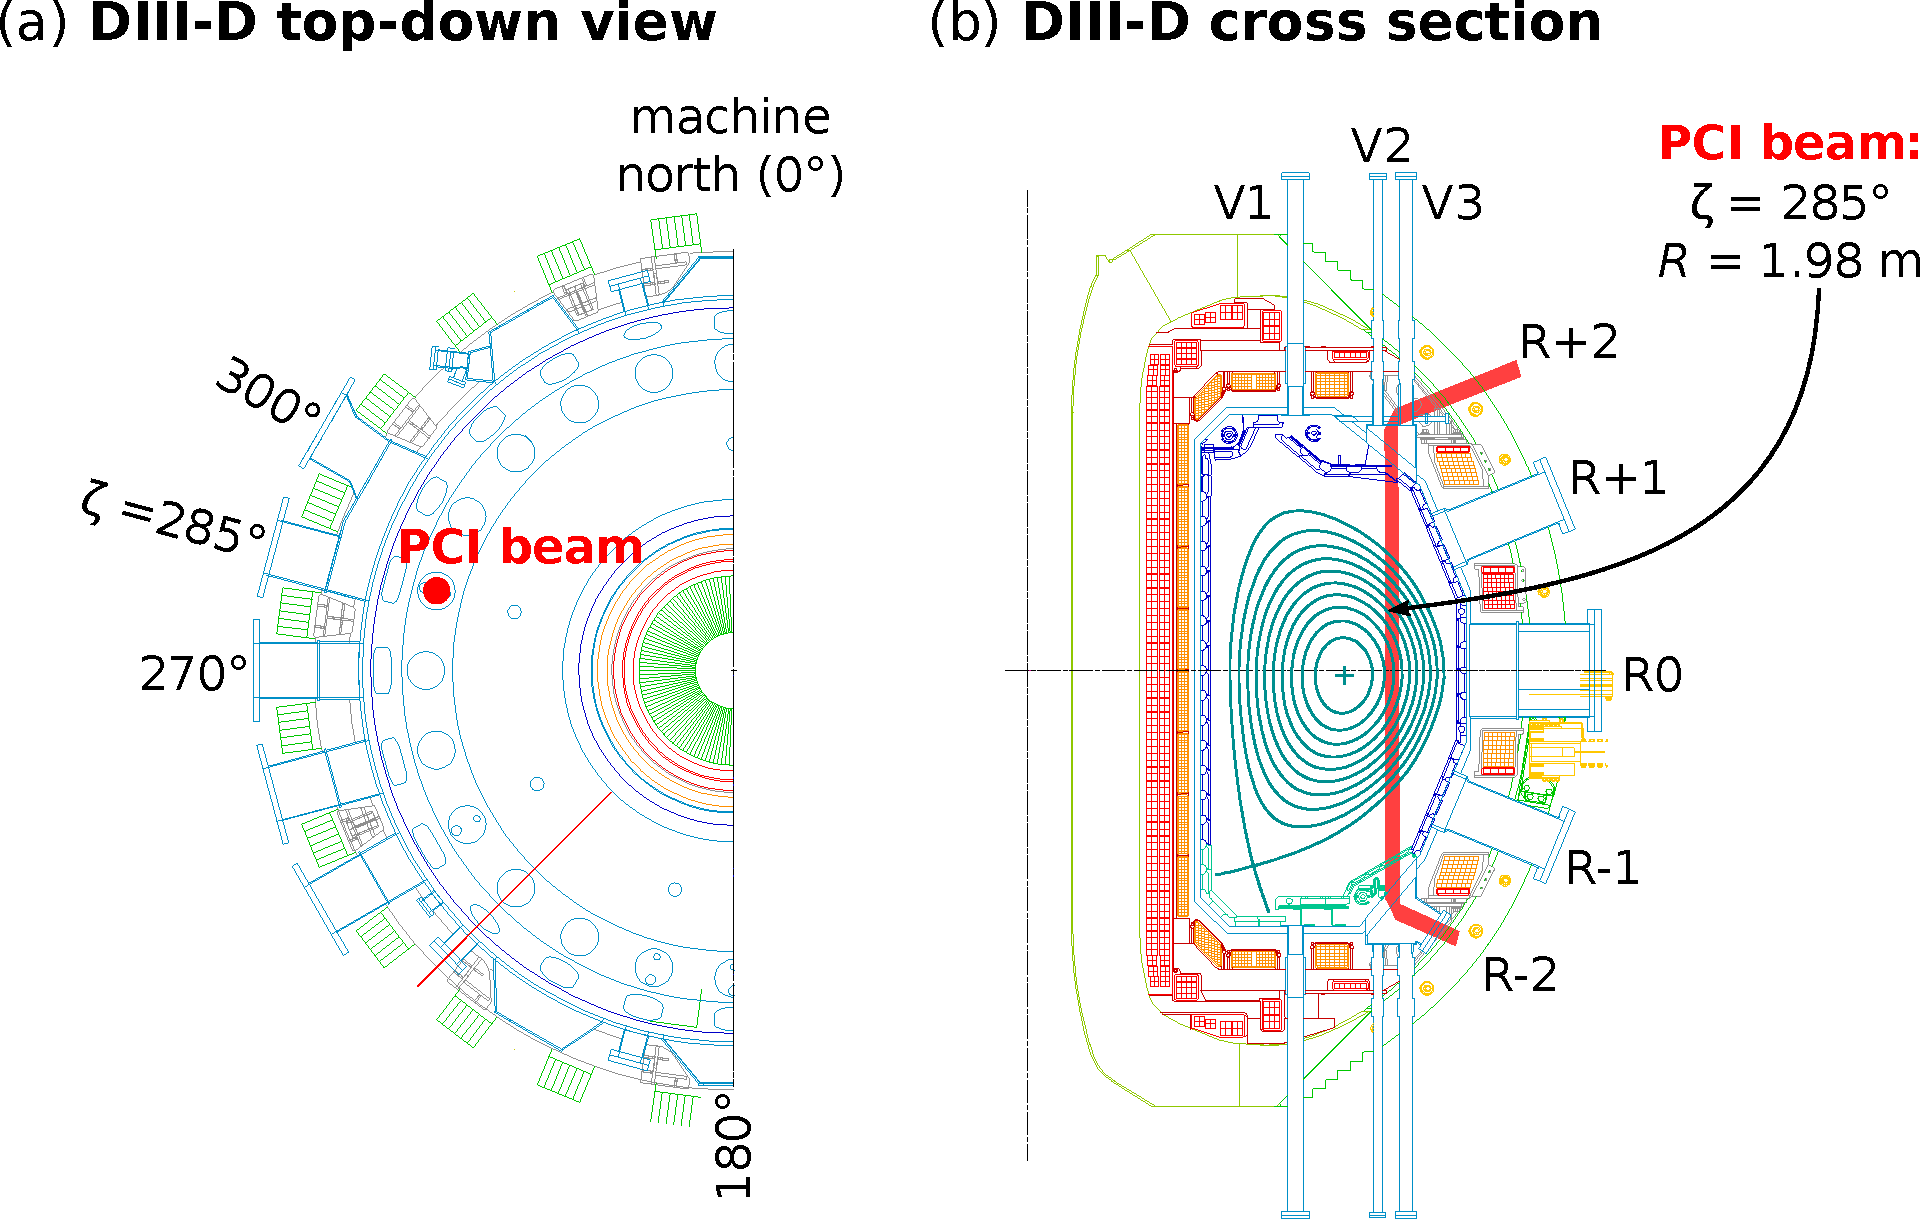
\includegraphics[width = \textwidth]{%
    Chapters/Implementation/figs/d3d_port_locations.pdf}
  \caption[\diiid \space port-labeling conventions and location of PCI]{%
    (a) View of \diiid \space from above,
    indicating the toroidal-labeling convention.
    (b) View of \diiid \space cross section,
    indicating the labeling convention
    for vertical (V) and radial (R) sightlines.
    The PCI beam enters the vessel through the $285^{\circ}$ R+2 port,
    propagates vertically downwards through the plasma
    at a major radius of $R = \SI{1.98}{\meter}$, and
    exits the vessel through the $285^{\circ}$ R-2 port.}
\label{fig:Implementation:d3d_port_locations}
\end{figure}


\section{\diiid's pre-existing PCI system}
The \diiid \space PCI system is
thoroughly described elsewhere~\cite{dorris_rsi09, dorris_phd}, but
the system components of relevance to this work
are briefly summarized below for completeness.


\subsection{System geometry}
The system is currently configured
in the ``Phase II'' geometry~\cite{dorris_rsi09},
with the probe beam propagating vertically downwards
from the $285^{\circ}$ R+2 port to the $285^{\circ}$ R-2 port.
The beam center sits at $R = $ \SI{1.98}{\meter}.
Both the toroidal and radial positions
of the PCI beam are shown in
Fig.~\ref{fig:Implementation:d3d_port_locations}.

The PCI system's vertical beam path constrains
which types of fluctuations it can and cannot detect.
Namely, the PCI-measured power fluctuations
(\ref{eq:InterferometricMethods:PCI_ratio_fluctuating_to_equilibrium_power})
correspond to \emph{line-integrated} electron-density fluctuations, which
are the physical origin of the phase fluctuations $\tilde{\phi}$ in
(\ref{eq:InterferometricMethods:phase_fluctuation}).
Because it is a line-integrated measurement,
only fluctuations propagating perpendicular to the beam path can be detected,
as fluctuations propagating parallel to the beam path
are effectively averaged out of the signal
\graffito{\textcolor{red}{what about $\delta \omega$?}}
(and, at a more fundamental level, fluctuations propagating
parallel to the beam path do \emph{not} spatially scatter the probe beam).
\graffito{\textcolor{red}{citation? Wesson?}}
Now, electrostatic turbulence (e.g.\ ITG, ETG) tends to be field-aligned
such that $k_{\perp} \gg k_{||}$, where
the $\perp$ and $||$ subscripts are used here to indicate
orientations that are perpendicular to and parallel to
the local magnetic field, respectively.
To lowest order, then, electrostatic fluctuations propagate
perpendicular to a tokamak's toroidal field.
PCI's vertical beam path and
the field-aligned constraint of electrostatic turbulence
imply that PCI is predominantly sensitive to fluctuations
with finite major-radial wavenumber $k_R$.
Thus, PCI's 32-element, 1-dimensional detector array
is oriented in the image plane such that
each detector element corresponds to a unique major radius in the plasma.

In some situations, spatially filtering ``masks''
\cite{dorris_rsi09, dorris_phd, lin_rsi06} or
2-dimensional detector arrays
\cite{sanin_rsi04, tanaka_rsi16}
can be used to localize measurements
by exploiting the spatial variation
in the magnetic field's orientation along the beam path.
These localization techniques typically work best
for high-$k$ measurements.
Note that $k_R$ is related to the
often-theoretically-relevant poloidal wavenumber $k_{\theta}$ via
\begin{equation}
  k_R = k_{\theta} \csc[\alpha(R, z)],
  \label{eq:Implementation:kR_to_ktheta}
\end{equation}
where $\alpha(R, z)$ is the angle
between the beam path and the local flux surface,
as shown schematically in
Fig.~\ref{fig:Implementation:relating_kR_to_ktheta}.
Of course, the fluctuation measurements must be localized,
either via direct measurement
(with 2-dimensional detector arrays or ``masks'')
or via inference from other plasma properties,
before (\ref{eq:Implementation:kR_to_ktheta})
can be inverted to yield $k_{\theta}$
from measured values of $k_R$.

\begin{figure}
  \centering
  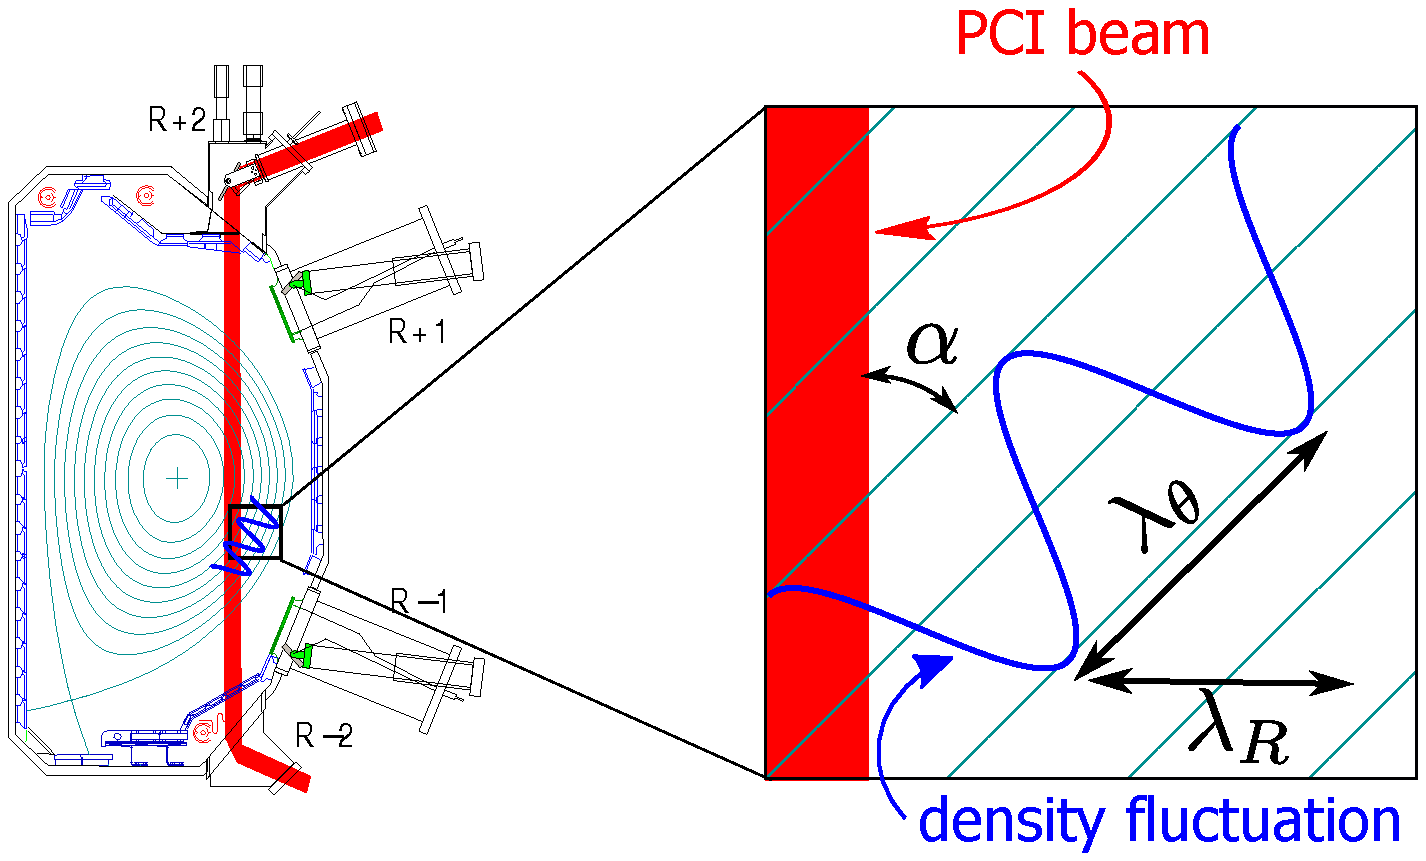
\includegraphics[width = 0.9 \textwidth]{%
    Chapters/Implementation/figs/kR_to_ktheta.pdf}
  \caption[Relating $k_R$ to $k_{\theta}$]{%
    The major-radial wavenumber $k_R = 2 \pi / \lambda_R$ and
    the poloidal wavenumber $k_{\theta} = 2 \pi / \lambda_{\theta}$
    are related via $\alpha(R, z)$, which
    is the angle between PCI's vertical probe beam and
    the local flux surface.}
\label{fig:Implementation:relating_kR_to_ktheta}
\end{figure}


\subsection{Spatial bandwidth}
Several critical wavenumbers were defined in
Section~\ref{sec:InterferometricMethods:pci} that
characterize the spatial bandwidth of a PCI system.
The goal of this section is to evaluate each of these
wavenumbers with the relevant parameters from
the \diiid \space PCI system.

PCI's low-$k$ cutoff, $k_g$, is physically constrained by
the free-space diffraction of the in-vessel probe beam.
This constraint was derived both
by examining the far-field overlap of the scattered and unscattered beams as in
(\ref{eq:InterferometricMethods:kmin_for_far_field_beam_separation}) and
by matching the spot size of the focused, unscattered beam
on the phase plate with the width of the phase plate's groove as in
(\ref{eq:InterferometricMethods:pci_kmin_physics}).
Both approaches yield the identical constraint that
$k_g^{\text{min}} = 2 / w_0$, where
$w_0$ is the 1/e $E$ radius of the in-vessel probe beam.
Capping aperture diffraction at acceptably small levels, however,
yields constraint
(\ref{eq:InterferometricMethods:aperture_radius_for_minimal_diffraction})
on $w_0$.
Now, after beam expansion and collimation,
the smallest aperture prior to beam-plasma interaction
is the $285^{\circ}$ R+2 port window,
which has a diameter of $4"$.
Thus, the beam expansion optics are configured to produce
to produce the widest possible beam
\begin{equation}
  w_0 = 4/3" \approx \SI{3.4}{\centi\meter}
\end{equation}
and the smallest physical constraint on the PCI low-$k$ cutoff
\begin{equation}
  k_g^{\text{min}} \approx \SI{0.6}{\per\centi\meter}
  \label{eq:Implementation:kg_min}
\end{equation}
while introducing negligible aperture diffraction.

PCI's \emph{realized} low-$k$ cutoff, however,
is typically $\sim 2-3 \times$ larger than
the diffraction-limited $k_g^{\text{min}}$.
This occurs if the width of the phase-plate groove
is oversized relative to the focused, unscattered beam spot, and
the realized low-$k$ cutoff is given by
(\ref{eq:InterferometricMethods:pci_kmin_engineering}).
Despite sacrificing some of the system's low-$k$ range,
operating with an oversized phase-groove width can be advantageous
on large, vibration-prone fusion experiments.
To see this, recall that the phase groove typically reflects
only a fraction $\eta < 1$ of the incident unscattered beam power
(the forward-facing surface of the \diiid \space phase-plate groove
is uncoated ZnSe, which has $\eta = 0.17$ at $\SI{10.6}{\micro\meter}$);
if vibration-induced misalignments
push the unscattered beam out of the phase groove,
there will be large power modulations on the PCI detector
that are \emph{not} attributable to plasma fluctuations and
that push the detector beyond its saturation limits.
While \diiid's PCI system has an elaborate feedback control system
that dynamically centers the unscattered beam on the phase-plate groove
\cite[Sec.~3.5]{coda_phd},
operating with an oversized phase-groove width
increases the size of the ``targeted'' operating space,
effectively giving the feedback system some leeway.
As such, the groove width of the \diiid \space phase plate is
\begin{equation}
  d = \SI{1}{\milli\meter},
\end{equation}
and the scattered beams are focused onto the phase plate by
an off-axis parabolic mirror of focal length
\begin{equation}
  f = 80.7"
\end{equation}
such that the realized low-$k$ cutoff
(\ref{eq:InterferometricMethods:pci_kmin_engineering})
becomes
\begin{equation}
  k_g \approx \SI{1.5}{\per\centi\meter},
\end{equation}
approximately $2.5 \times$ larger than
the diffraction-limited minimum in (\ref{eq:Implementation:kg_min}).

PCI's high-$k$ limits are dictated by
finite-sized collection optics and system magnification.
The \diiid \space phase plate has a diameter
\begin{equation}
  D = 2"
\end{equation}
such that the phase plate's high-$k$ cutoff
(\ref{eq:InterferometricMethods:pci_kmax_engineering})
is
\begin{equation}
  k_D \approx \SI{75}{\per\centi\meter}.
\end{equation}
Although the $5"$ diameter $285^{\circ}$ R-2 exit window and
the subsequent $12"$ diameter steering mirrors
are large enough to accommodate beams scattered
from fluctuations with wavenumbers $|k| \sim k_D$,
apertures in the imaging optics
only allow beams scattered from fluctuations with
\begin{equation}
  |k| \lesssim \SI{20}{\per\centi\meter}
\end{equation}
to reach the PCI detector.
Upon reaching the detector,
the measured PCI signal is subject to finite sampling-volume effects,
which result from spatial averaging over the face of a detector element.
The PCI's 32-element, 1-dimensional detector array have elements
of height $\SI{1}{\milli\meter}$, width
\begin{equation}
  s_x^{\text{pci}} = \SI{0.5}{\milli\meter},
\end{equation}
and center-to-center element spacing of $\SI{0.55}{\milli\meter}$.
Coupled with the system's magnification
\graffito{\textcolor{red}{Correct? Sign?}}
\begin{equation}
  |M^{\text{pci}}| \approx 0.5,
\end{equation}
the finite sampling-volume cutoff
(\ref{eq:InterferometricMethods:finite_sampling_volume_cutoff})
of the PCI is
\begin{equation}
  k_{\text{fsv}}^{\text{pci}} \approx \SI{63}{\per\centi\meter}.
\end{equation}


\subsection{Temporal bandwidth}
PCI's detector (Infrared Associates MCT-16-32) and
its associated preamplifiers (also through Infrared Associates)
are the dominant constraint on the system's temporal bandwidth.
The HgCdTe detector array
operates in the photoconductive regime and
is cooled by liquid nitrogen;
the liquid-nitrogen cooling reduces noise and boosts the response such that
the detector-preamplifier combination has
a specific detectivity
$D^* \approx \SI{2e10}{\centi\meter \sqrt\hertz \per\watt}$ and
a $\SI{500}{\volt\per\watt}$ responsivity
to incident $\SI{10.6}{\micro\meter}$ light
(note that the detector also has a saturation intensity
$I_{\text{sat}} \sim \SI{1}{\milli\watt \per\milli\meter\squared}$).
The benefits of cooling, however, come at the expense of reduced bandwidth:
the detector-preamplifier combination has
a high-frequency, 2-pole cutoff
at $\sim \SI{800}{\kilo\hertz}$~\cite{rost_pci_detector_response}.
As the DC PCI signal is of little interest,
the detector-preamplifier combination also has
a low-frequency, 1-pole cutoff
at $\sim \SI{2}{\kilo\hertz}$~\cite{rost_pci_detector_response}.

The components downstream of the detector and preamplifiers
have a small impact on the system bandwidth, but
they are briefly summarized below for completeness.
The Variable Gain and Filter (VGAF) circuits~\cite[Sec.~3.3.3]{dorris_phd}
are located immediately downstream of the preamplifiers and
have a low-frequency, 1-pole cutoff that can be easily switched between
$\SI{10}{\kilo\hertz}$ and $\SI{100}{\kilo\hertz}$;
the VGAFs are typically operated in the $\SI{10}{\kilo\hertz}$ configuration.
Following the VGAFs,
fiber optic links (Analog Modules 732 T/R-2.5-33k)
with an analog bandwidth of DC to $\SI{10}{\mega\hertz}$
transmit the signal from the \diiid \space pit to the annex.
Upon reaching the annex,
the signals are digitized with two of D-tAcq's ACQ216CPCI boards,
typically at a sampling rate of $f_s = 4 \, \text{MSPS}$.


\section{Component replacement}
Over the course of this work,
several components crucial to the operation of the PCI
(and the soon-to-be-described interferometer)
failed.
The failures and replacements are briefly described below.


\subsection{Quadrature detector for beam-position feedback}
A quadrature detector measures the position
of the unscattered beam on the phase plate,
providing the input to the feedback control system
that dynamically centers the unscattered beam
on the phase-plate groove~\cite[Sec.~3.5]{coda_phd}.
As the quadrature detector
cannot physically be co-located with the phase plate,
a beam splitter samples the unscattered beam
immediately upstream of the phase plate, and
a single lens \emph{images} onto the quadrature detector
the point in the sampled beam that corresponds to the phase-plate location.
Thus, beam movement on the phase plate is mirrored
by movement of the sampled beam on the quadrature detector.
System response is maximized
with imaging magnification $|M| \approx 1$
(relative to the beam size at the phase plate) and
incident optical intensities $I_{\text{opt}}$
well beyond the linear saturation intensity
(i.e. $I_{\text{sat}} \ll I_{\text{opt}} < I_{\text{dam}}$)
~\cite{marinoni_FB_detector_report}~\cite[Sec.~3.5(b)]{coda_phd}.

The old quadrature detector consisted of four
photoconductive, liquid-nitrogen cooled, HgCdTe elements.
Quadrature detectors for use at $\SI{10.6}{\micro\meter}$
had only just become commercially available
when this unit was procured from Belov Technology in the mid-1990s
~\cite[Sec.~3.5(b)]{coda_phd}.
Cooling HgCdTe can
extend the long-wavelength cutoff beyond $\SI{10.6}{\micro\meter}$,
reduces noise, and
increases responsivity~\cite{vigo_catalog}.
In particular, HgCdTe's responsivity increases by $\sim 10^3$
when cooled to liquid-nitrogen temperatures such that
that the incident optical signal
exceeds the $1 / f$ noise
characteristic of photoconductive detectors~\cite{vigo_catalog}.
As the bandwidth requirements for the PCI feedback system
extend from DC to $\lesssim \SI{10}{\kilo\hertz}$,
$1 / f$ noise cannot be easily combated by
e.g.\ mechanically chopping the beam.
After $\sim 20$ years of operation,
the old quadrature detector failed in December 2014,
presumably having reached its expected lifetime.
As Belov Technology no longer exists,
it was not possible to procure a drop-in replacement.
Fortunately, in the context of position sensing,
HgCdTe technology has significantly improved since the mid-1990s.

The new quadrature detector
(four VIGO PVM-10.6 elements mounted on a VIGO QIP preamplifier)
is in many ways superior to the old quadrature detector.
This superiority stems from VIGO's use of
``multiple heterojunction'' HgCdTe detector elements~\cite{vigo_catalog},
which endow the detector with several advantageous properties.
First, the detector is photovoltaic.
Thus, the detector is \emph{not} plagued by the $1 / f$ noise
characteristic of photoconductive detectors.
Second, the detector's long-wavelength cutoff
sits beyond $\SI{10.6}{\micro\meter}$ at room temperature.
Taken together, the above two properties imply that
the new quadrature detector can be operated at room temperature,
i.e.\ it does \emph{not} need to be cooled by liquid nitrogen.
Lacking a dewar, the new quadrature detector
is much smaller than the old quadrature detector;
the new detector can also be mounted with an arbitrary orientation,
whereas the dewar of the old detector required an upright orientation.
This new-found flexibility substantially opened
the optical design space for the feedback arm and
the plasma arm of the soon-to-be-described interferometer.
Additionally, the dewar of the old quadrature detector
only had a $\sim \SI{6}{\hour}$ hold time,
which is not sufficient for a full day of \diiid \space operations;
thus, the use of a room-temperature quadrature detector has
eliminated the mid-day ``pit runs'' to refill the quadrature detector's dewar,
allowing easier operation of the system.
Although room-temperature operation reduces
the detector's specific detectivity to
$D^* \sim \SI{e7}{\centi\meter \sqrt\hertz \per\watt}$
(roughly three orders of magnitude \emph{lower} than
that of the old quadrature detector),
the optical signal corresponds to the strong, unscattered probe beam
(as opposed to e.g.\ weak beams
scattered from small-amplitude plasma fluctuations), so
the increase in noise negligibly influences operation of the feedback system.

\begin{itemize}
  \item When was new detector acquired?
  \item \textcolor{red}{Picture}
  \item \textcolor{red}{Table of properties (?)}
\end{itemize}


\subsection{CO$_2$ laser}
The old CO$_2$ laser~\cite[Sec.~3.3]{coda_phd},
manufactured by MPB Technologies,
had been in service since
the inception of the \diiid \space PCI system in the mid-1990s.
Lasing occurred via high voltage, DC-excitation
inside of a $\SI{2}{\meter}$-long, sealed-off glass tube
to produce a TEM$_{00}$ (Gaussian) mode with linear polarization.
The laser nominally had
a $\lesssim \SI{300}{\kilo\hertz}$ frequency stability
over short time windows ($\SI{0.1}{\second}$) and
a $\lesssim \SI{3}{\mega\hertz}$ frequency stability
over longer time windows ($\SI{e3}{\second}$).
The laser's tube was replaced in late 1999
when a precipitous drop in beam power indicated imminent failure.
Following the tube's replacement,
the measured beam power consistently hovered at $\sim\SI{14}{\watt}$
for many years.
However, in early 2016, the beam power again precipitously dropped.
The laser's high voltage power supply,
which was replaced in 2005 after failing,
was tested and found to be operating nominally,
suggesting that the drop in beam power
was attributable to the laser's aging tube.
Unfortunately, MPB Technologies has abandoned its efforts in CO$_2$ lasers
and was unable to replace or repair the tube.
Third-party tube repair was investigated but
ultimately deemed unacceptable due to
the required lead times and the lack of a guaranteed repair.
Fortunately, the MPB laser continued operating, albeit at reduced power,
throughout the 2016 campaign, allowing continued diagnostic development
of the soon-to-be-described interferometer.

After an exhaustive search of the CO$_2$-laser market,
a water-cooled AL30ST CO$_2$ laser was procured
from Access Laser Company (Everett, WA) in mid-2016.
Lasing occurs via RF excitation at $\SI{40.68}{\mega\hertz}$;
RF excitation requires far-lower voltages than DC excitation,
eliminating the high-voltage safety risk and allowing more efficient lasing
\cite{he_jap83}.
As in the old MPB laser,
the lasing cavity is supported by carbon fiber rods (rather than Invar)
to mitigate any effects of the tokamak's large, ambient magnetic fields
on the laser's performance.
The laser oscillates on a TEM$_{00}$ (Gaussian) mode (spec'd $M^2 < 1.1$)
with vertical polarization (spec'd extinction ratio $1 / 897$), and
its $\SI{37}{\watt}$ power output is stable to within $\pm 1.1\%$
\cite{marinoni_AL30ST_report}.
Lasing occurs on the $P(20)$ line
of the $00^{\circ}1 \rightarrow 10^{\circ}0$ transition
to produce radiation with a vacuum wavelength of
$\lambda_0 = \SI{10.591}{\micro\meter}$.
Measurements with wavelength meter 621B
from Bristol Instruments, Inc. (Victor, NY)
indicate that the laser's wavelength stability over several seconds
is characterized by a Voigt distribution with
full width at half maximum of $\SI{0.0029}{\nano\meter}$, which
corresponds to a frequency stability (over \emph{several seconds})
of $\SI{3.8}{\mega\hertz}$ \cite{marinoni_AL30ST_report}.

In the context of measuring plasma-density fluctuations
with an external reference-beam interferometer,
the relevant metric is the laser's frequency stability
over much shorter time windows
(i.e.\ the time difference corresponding to
the difference in optical path length between
the interferometer's plasma and reference arms).
This is most easily evaluated empirically
by deploying the laser in the given interferometric system
and evaluating the corresponding phase noise.
Successive test shots,
the first with the old MPB laser and the second with the AL30ST,
show comparable phase noise (and hence frequency stability)
between the two lasers.
Thus, the AL30ST frequency stability is deemed to be sufficient
for measurement of plasma-density fluctuations
with the soon-to-be-described external reference-beam interferometer.

\begin{itemize}
  \item \textcolor{red}{Picture}
  \item \textcolor{red}{Fig. of new vs.\ old laser stability}
\end{itemize}


\subsection{In-vessel mirrors}
Two of the PCI mirrors are located
\emph{inside} of the \diiid \space vacuum vessel.
As indicated in Fig.~\ref{fig:Implementation:d3d_port_locations}(b),
the PCI probe beam enters the machine through the $285^{\circ}$ R+2 port,
reflects off of the first in-vessel mirror,
propagates vertically downwards through the machine (and the plasma),
reflects off the second in-vessel mirror, and
exits the machine through the $285^{\circ}$ R-2 port.
The in-vessel mirrors are elongated
along the axis parallel to the plane of incidence
in order to increase the mirrors' apparent surface area.
The mirrors were fabricated by Esco Optics, Inc. (Oak Ridge, NJ).
The mirrors are made of fused quartz with
a reflective aluminum surface and a protective SiO coating.

In mid-2015 the beam quality of the CO$_2$ laser and the HeNe alignment laser
after passing through the \diiid \space vessel was noted to be poor
(i.e. substantially non-Gaussian).
Numerous tests suggested that the poor beam quality was attributable
damaged in-vessel mirrors;
this hypothesis was confirmed via visual inspection
during the next manned entry of the machine.
``Drop-in'' replacements were ordered from Esco Optics
and were installed in mid-2016.
The removed, damaged mirrors are shown in
Fig.~\ref{fig:Implementation:in_vessel_mirrors}.
It is not known whether the mirrors were damaged
during e.g. plasma operations or high-temperature bakes of the vessel.

\begin{figure}
  \centering
  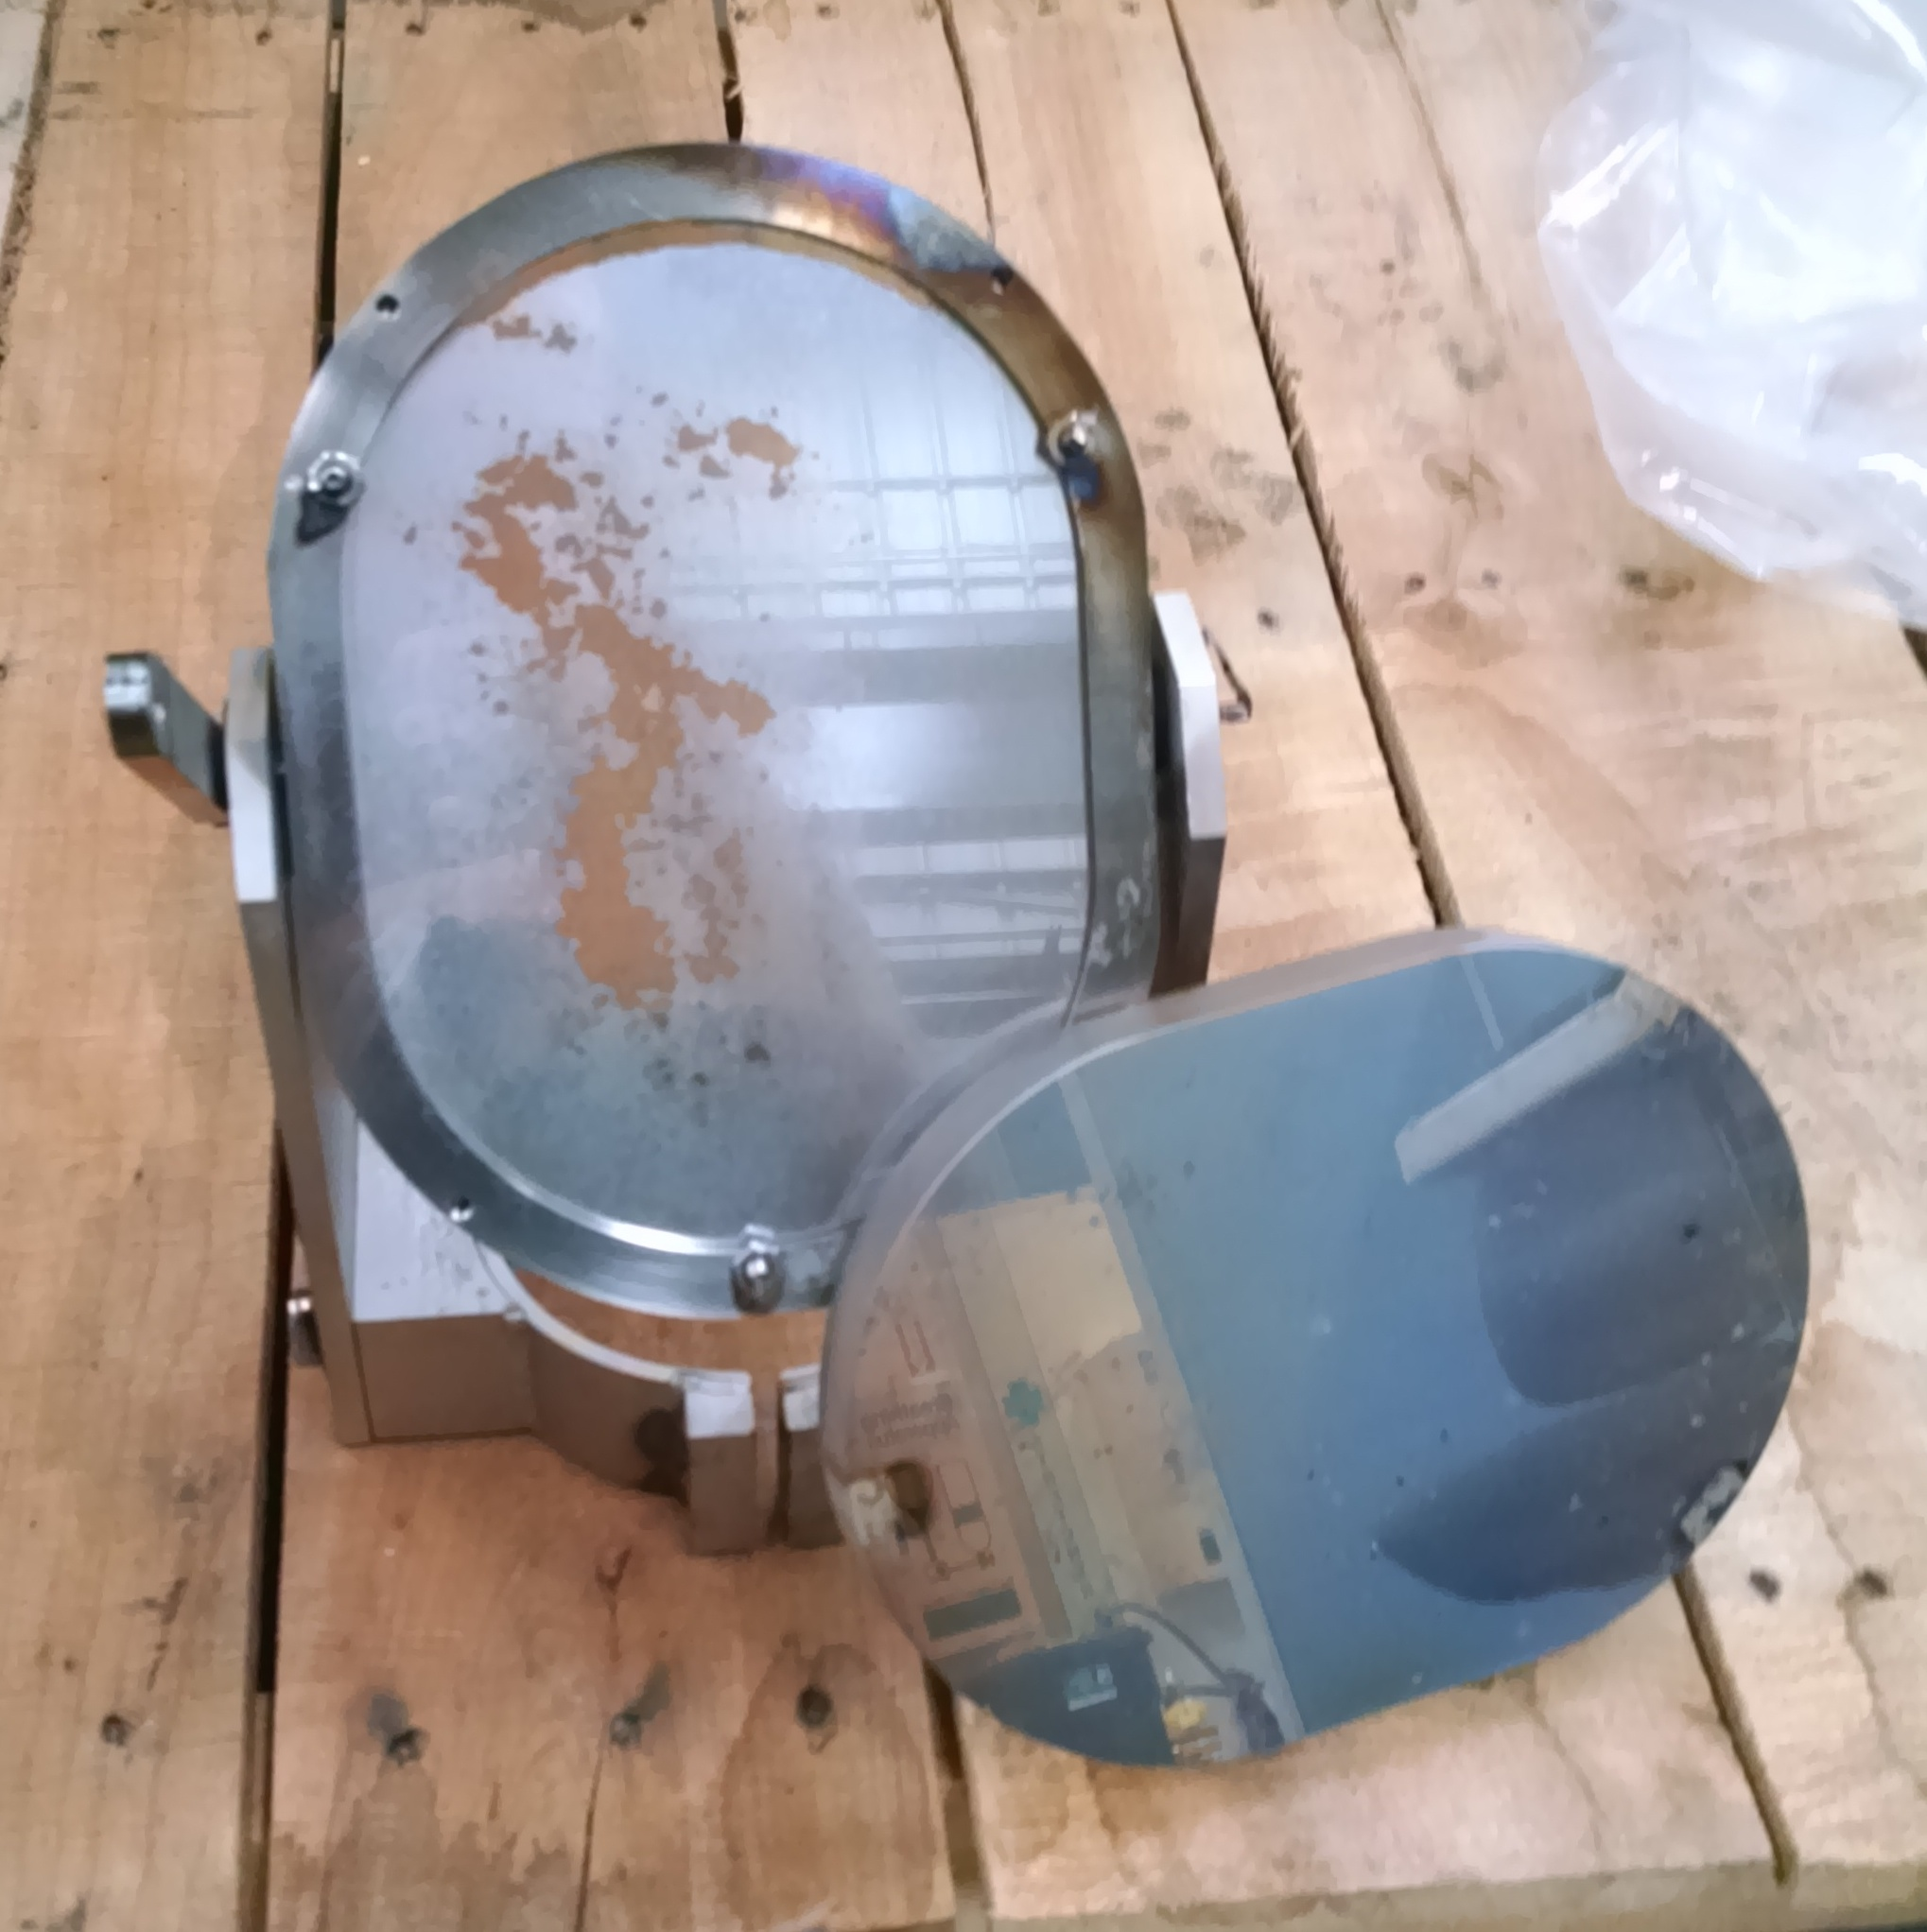
\includegraphics[width = 0.6 \textwidth]{%
    Chapters/Implementation/figs/in_vessel_mirrors.jpg}
  \caption[PCI's damaged in-vessel mirrors]{%
    PCI's damaged in-vessel mirrors, sitting
    in the \diiid \space ``Hi-Bay''
    after removal from the vessel in mid-2016.
    (Note that the reflectivity of each mirror at $\SI{10.6}{\micro\meter}$
    cannot be gauged from this photograph in the visible spectrum).
    ``Drop-in'' replacements were installed
    before the resumption of plasma operations.}
\label{fig:Implementation:in_vessel_mirrors}
\end{figure}


\section{Interferometer design study}


\subsection{Expected noise}

\begin{itemize}
  \item Demodulated NEP from
    (\ref{eq:DesignConsiderations:demodulated_NEP_spectral_density}) gives
    $\sim \SI{e-18}{\watt\squared\per\hertz}$
  \item Demodulated shot noise from
    (\ref{eq:DesignConsiderations:demodulated_shot_noise_spectral_density})
    gives $\sim \SI{e-21}{\watt\squared\per\hertz}$
\end{itemize}


\section{Interferometer component selection}
\subsection{Acousto-optic modulator}
\subsection{Imaging optics}
\subsection{Detector}
\subsection{Electronics}
\begin{itemize}
  \item Automatic gain-control amplifier
  \item Analog I/Q demodulator
  \item Low-frequency ``audio'' amplifiers
\end{itemize}
\subsection{Digitizer}
\begin{itemize}
  \item Bit noise
\end{itemize}


\section{Optical layout}
\begin{itemize}
  \item ``Build-ability'',
  \item $M$, magnification for wavenumber response,
  \item $C$, for stability to FB, and
  \item $\delta \phi_{\kappa}$
\end{itemize}


\section{Fighting phase noise}
\subsection{Local oscillator stability}


\section{Sound-wave calibration of combined PCI-interferometer}
\subsection{Sound-wave characterization}
\subsection{Measurements}
\begin{itemize}
  \item Wavenumber range
  \item Cross calibration
  \item System sensitivity
\end{itemize}

\begin{table}[ht]
  \centering
  \renewcommand{\arraystretch}{1.5}% Spread rows out...
  \begin{tabular}{%
    >{\centering}m{3.0cm} >{\centering}m{4.5cm} >{\centering}m{4.5cm}
  }
    \toprule%
    \textbf{Parameter} & \textbf{PCI} & \textbf{Interferometer}
    \tabularnewline%
    \midrule
    \textbf{probe beam} & single CO$_2$ beam & single CO$_2$ beam
    \tabularnewline%
    \textbf{frequency bandwidth}
    & \SI{10}{\kilo\hertz} $ < f < $ \SI{2}{\mega\hertz}
    & \SI{10}{\kilo\hertz} $ < f < $ \SI{2}{\mega\hertz}
    \tabularnewline%
    \textbf{spatial bandwidth}
    & \SI{1.5}{\centi\meter}\ts{-1} $ < k < $ \SI{20}{\centi\meter}\ts{-1}
    & \SI{0}{\centi\meter}\ts{-1} $ < k < $ \SI{5}{\centi\meter}\ts{-1}
    \tabularnewline%
    \toprule%
  \end{tabular}
  \caption[Parameters of \diiid's combined PCI-interferometer]{%
    PCI and interferometry have compatible probe beams, comparable
    frequency bandwidths, and \emph{complementary} spatial bandwidths.
    All parameters are for DIII-D's currently implemented PCI--interferometer
    system.
  }%
\label{table:Implementation:PCI_interferometer}
\end{table}


\section{Looking towards ITER\ldots}


\bibliographystyle{plainurl}
\bibliography{references}
%
\newcommand{\meas}{\text{meas}}
\newcommand{\nom}{\text{nom}}
\newcommand{\trig}{\text{trig}}
\newcommand{\Ny}{\text{Ny}}


\chapter{Correlation of \diiid's toroidally separated interferometers}
\label{ch:ToroidalCorrelation}
The toroidal structure of an MHD mode can have important implications
for the mode's stability and its interaction with the surrounding plasma.
A mode's toroidal structure is typically characterized
by its toroidal mode number $n$.
Historically, measurement of toroidal (and poloidal) mode numbers
with external magnetic probes has provided rich insight
into the physics governing numerous operational regimes and stability limits.
However, core-localized MHD produces weak signals outside of the plasma volume,
making measurement of the corresponding mode numbers
via external magnetic probes difficult or impossible.
Recently, measurements from toroidally separated
electron cyclotron emission imaging (ECEI) systems
on the KSTAR tokamak have identified mode numbers of
sawteeth~\cite{choe_nf_2015},
demonstrating the utility of using more exotic measurements
to probe the structure of core-localized MHD.

This chapter describes the correlation
of toroidally separated interferometers
to measure toroidal mode numbers.
To the author's knowledge,
this is the first such implementation in a tokamak.
As the interferometers are capable of probing the plasma core,
their correlation allows direct measurement
of the toroidal structure of core-localized modes
--- a long-sought after and first-of-its-kind measurement at \diiid.
Below, Section~\ref{sec:ToroidalCorrelation:TwoPointCorrelation}
reviews the two-point correlation technique,
which allows inference of a propagating wave's
spatial structure from measurements
made at two distinct spatial locations.
Section~\ref{sec:ToroidalCorrelation:Interferometers}
then examines the geometry of the interferometers and
develops a formula for the measured toroidal mode number.
Section~\ref{sec:ToroidalCorrelation:ImplementationDetails}
describes the careful efforts to eliminate timebase discrepancies
between the two interferometer systems,
validates the interferometer-measured toroidal mode numbers
against those measured by external magnetic probes, and
discusses the effect of the interferometers' radial offset.
Finally, Section~\ref{sec:ToroidalCorrelation:CoreLocalized}
provides an encouraging proof of principle
regarding the ability of the correlated interferometers
to diagnose core-localized MHD.


\section{Two-point correlation}
\label{sec:ToroidalCorrelation:TwoPointCorrelation}
Two-point correlation allows inference
of a propagating wave's spatial structure
from measurements made at two distinct spatial locations.
Below,
Section~\ref{sec:ToroidalCorrelation:TwoPointCorrelation:wavenumber_measurement}
details the two-point correlation technique.
Section~\ref{sec:ToroidalCorrelation:TwoPointCorrelation:aliasing}
then discusses the aliasing of large wavenumbers and
establishes a measurement's Nyquist wavenumber,
below which wavenumbers are \emph{not} aliased.
Finally,
Section~\ref{sec:ToroidalCorrelation:TwoPointCorrelation:toroidal_mode_numbers}
converts the results of the previous sections
into their toroidal-mode-number equivalents,
as is conventional for fluctuation characterization in a tokamak.


\subsection{Wavenumber measurement via two-point correlation}
\label{sec:ToroidalCorrelation:TwoPointCorrelation:wavenumber_measurement}
Consider a $1$-dimensional, coherent density fluctuation
with amplitude $\tilde{n}_0$, wavenumber $k$, and angular frequency $\omega$
\begin{equation}
  \tilde{n}(z, t)
  =
  \tilde{n}_0
  e^{i(k z - \omega t)}.
  \label{eq:ToroidalCorrelation:coherent_density_fluctuation}
\end{equation}
Imagine that the density is measured
at two locations separated by distance $\Delta z$,
producing two time series, $x(t)$ and $y(t)$, given as
\begin{align}
  x(t)
  &=
  \tilde{n}(z_0, t)
  \\
  y(t)
  &=
  \tilde{n}(z_0 + \Delta z, t)
  =
  x(t) e^{i k \Delta z}.
\end{align}
The cross phase $\alpha_{xy}$ between these two time series is
\begin{align}
  \alpha_{xy}
  &=
  \arg\left[ x^*(t) \cdot y(t) \right]
  \label{eq:ToroidalCorrelation:cross_phase}
  \\
  &=
  k \Delta z,
\end{align}
where $x^*$ is the complex conjugate of $x$.
Thus, a measured wavenumber $k_{\meas}$
can be inferred from the cross phase via
\begin{equation}
  k_{\meas} = \frac{\alpha_{xy}}{\Delta z}.
  \label{eq:ToroidalCorrelation:wavenumber_from_cross_phase}
\end{equation}
The cross phase $\alpha_{xy}$ of $x(t)$ and $y(t)$
can be readily estimated via
the non-parametric, FFT-based
spectral-estimation techniques discussed in
Appendix~\ref{app:SpectralEstimation:NonParametric}.
Note that such cross-phase estimates are frequency-resolved,
allowing simultaneous characterization
of multiple fluctuations at distinct frequencies.


\subsection{Aliasing \& the Nyquist wavenumber}
\label{sec:ToroidalCorrelation:TwoPointCorrelation:aliasing}
The measured wavenumber
(\ref{eq:ToroidalCorrelation:wavenumber_from_cross_phase})
may be \emph{aliased}.
To see this, note that the cross-phase estimate $\alpha_{xy}$
is only unique modulo $2 \pi$
(that is, $0$ is equivalent to $\pm 2 \pi$, $\pm 4 \pi$, etc.).
If the fluctuation wavenumber $k$ is sufficiently large
(i.e.\ if it exceeds the so-called Nyquist wavenumber $k_{\Ny}$),
this cross-phase ambiguity aliases the measured wavenumber
(\ref{eq:ToroidalCorrelation:wavenumber_from_cross_phase})
away from the true wavenumber.

In the most general case,
the wave's propagation direction is not known \emph{a priori}, and
both positive and negative wavenumbers should be considered
(i.e.\ $-\pi < \alpha_{xy} \leq \pi$).
This cross-phase domain yields a Nyquist wavenumber
\begin{equation}
  k_{\Ny} = \frac{\pi}{\Delta z},
  \qquad \text{for \emph{unknown} propagation direction.}
  \label{eq:ToroidalCorrelation:Nyquist_wavenumber_unknown_propagation}
\end{equation}
Wavenumber measurements
(\ref{eq:ToroidalCorrelation:wavenumber_from_cross_phase})
from fluctuations with $|k| > k_{\Ny}$ are aliased, while
measurements from fluctuations with $|k| \leq k_{\Ny}$ are not aliased.
Note that
(\ref{eq:ToroidalCorrelation:Nyquist_wavenumber_unknown_propagation})
is equivalent to the famed Nyquist frequency:
making the transformations $\Delta z \rightarrow 1 / f_s$
for temporal sampling rate $f_s$ and
$k \rightarrow 2 \pi f$,
(\ref{eq:ToroidalCorrelation:Nyquist_wavenumber_unknown_propagation})
readily becomes $f_{\Ny} = f_s / 2$.
Thus, $1 / \Delta z$ can be thought of as the spatial sampling rate,
with a larger sampling rate (i.e.\ smaller $\Delta z$)
allowing un-aliased measurements of larger wavenumbers.

Now, if the wave's propagation direction is known \emph{a priori}
(for example, if the wave propagation is dominated by advection, and
the fluid velocity is well-diagnosed),
only a single polarity of wavenumbers need to be considered.
For concreteness, positive wavenumbers are considered below
(i.e.\ $0 \leq \alpha_{xy} < 2 \pi$).
This cross-phase domain yields a Nyquist wavenumber
\begin{equation}
  k_{\Ny} = \frac{2 \pi}{\Delta z},
  \qquad \text{for \emph{known} propagation direction.}
  \label{eq:ToroidalCorrelation:Nyquist_wavenumber_known_propagation}
\end{equation}


\subsection{Measurement of toroidal mode numbers}
\label{sec:ToroidalCorrelation:TwoPointCorrelation:toroidal_mode_numbers}
Fluctuations in a torus are often characterized
by their toroidal $n$ and poloidal $m$ mode numbers,
both of which are constrained to be integers
by the toroidal and poloidal periodicities, respectively, of the torus.
For a torus with major radius $R$,
the toroidal mode number $n$ is related
to the toroidal wavenumber $k_{\zeta}$ as
\begin{equation}
  k_{\zeta} = \frac{n}{R},
\end{equation}
and the toroidal angular separation $\Delta \zeta$
is related to the spatial separation $\Delta z$ as
\begin{equation}
  \Delta \zeta = \frac{\Delta z}{R}.
\end{equation}
Using these definitions,
the above formulas for the measured wavenumber and the Nyquist wavenumber
can be rewritten in terms of toroidal mode numbers as follows:
\begin{align}
  n_{\text{meas}}
  &=
  \frac{\alpha_{xy}}{\Delta \zeta},
  \label{eq:ToroidalCorrelation:modenumber_from_cross_phase}
  \\
  n_{\text{Ny}}
  &=
  \begin{cases}
    \frac{\pi}{\Delta \zeta}
    \qquad \text{for \emph{unknown} propagation direction} \\
    \frac{2 \pi}{\Delta \zeta}
    \qquad \text{for \emph{known} propagation direction}
  \end{cases}.
  \label{eq:ToroidalCorrelation:Nyquist_modenumber}
\end{align}


\section{Toroidal correlation of interferometers}
\label{sec:ToroidalCorrelation:Interferometers}
This section applies two-point correlation
to the measurement of toroidal mode numbers
with \diiid's toroidally separated, heterodyne CO$_2$ interferometers.
Section~\ref{sec:ToroidalCorrelation:Interferometers:diiid}
describes the geometry of the interferometer probe beams,
which establishes the Nyquist toroidal mode number.
Sections~\ref{sec:ToroidalCorrelation:Interferometers:phase_fluctuations} and
\ref{sec:ToroidalCorrelation:Interferometers:interferometer_measured_mode_number}
then examine the relationship between
the interferometer-measured phase fluctuations and
the toroidal mode number.
As the interferometers are capable of probing the plasma core,
their correlation allows direct measurement
of the toroidal structure of core-localized modes
--- a long-sought after and first-of-its-kind measurement at \diiid.


\subsection{\diiid's interferometers}
\label{sec:ToroidalCorrelation:Interferometers:diiid}
\diiid's multichannel, two-color, heterodyne CO$_2$ interferometer
measures both the equilibrium~\cite{carlstrom_rsi88} and
fluctuating~\cite{vanzeeland_ppcf05, pace_nf17} components
of the line-integrated electron density.
Each channel is configured as a Michelson interferometer,
with each probe beam making a double-pass through the plasma.
The three vertical chords pass through the $V1$, $V2$, and $V3$ ports
at a toroidal location of $240^{\circ}$, while
the radial chord passes through the $R0$ port
at a toroidal location of $225^{\circ}$.
Of particular relevance to this work is the $V2$ interferometer,
which has a major-radial location $R = \SI{1.94}{\meter}$ and
is shown in Fig.~\ref{fig:ToroidalCorrelation:pci_interf_locs}.
The viewing geometry influences
an interferometer's sensitivity to various MHD instabilities;
for example, vertical chords are more sensitive to
toroidal Alfv\'{e}n eigenmodes (TAEs), while
radial chords are more sensitive to
reversed-shear Alfv\'{e}n eigenmodes (RSAEs)
\cite{vanzeeland_ppcf05}.

\begin{figure}
  \centering
  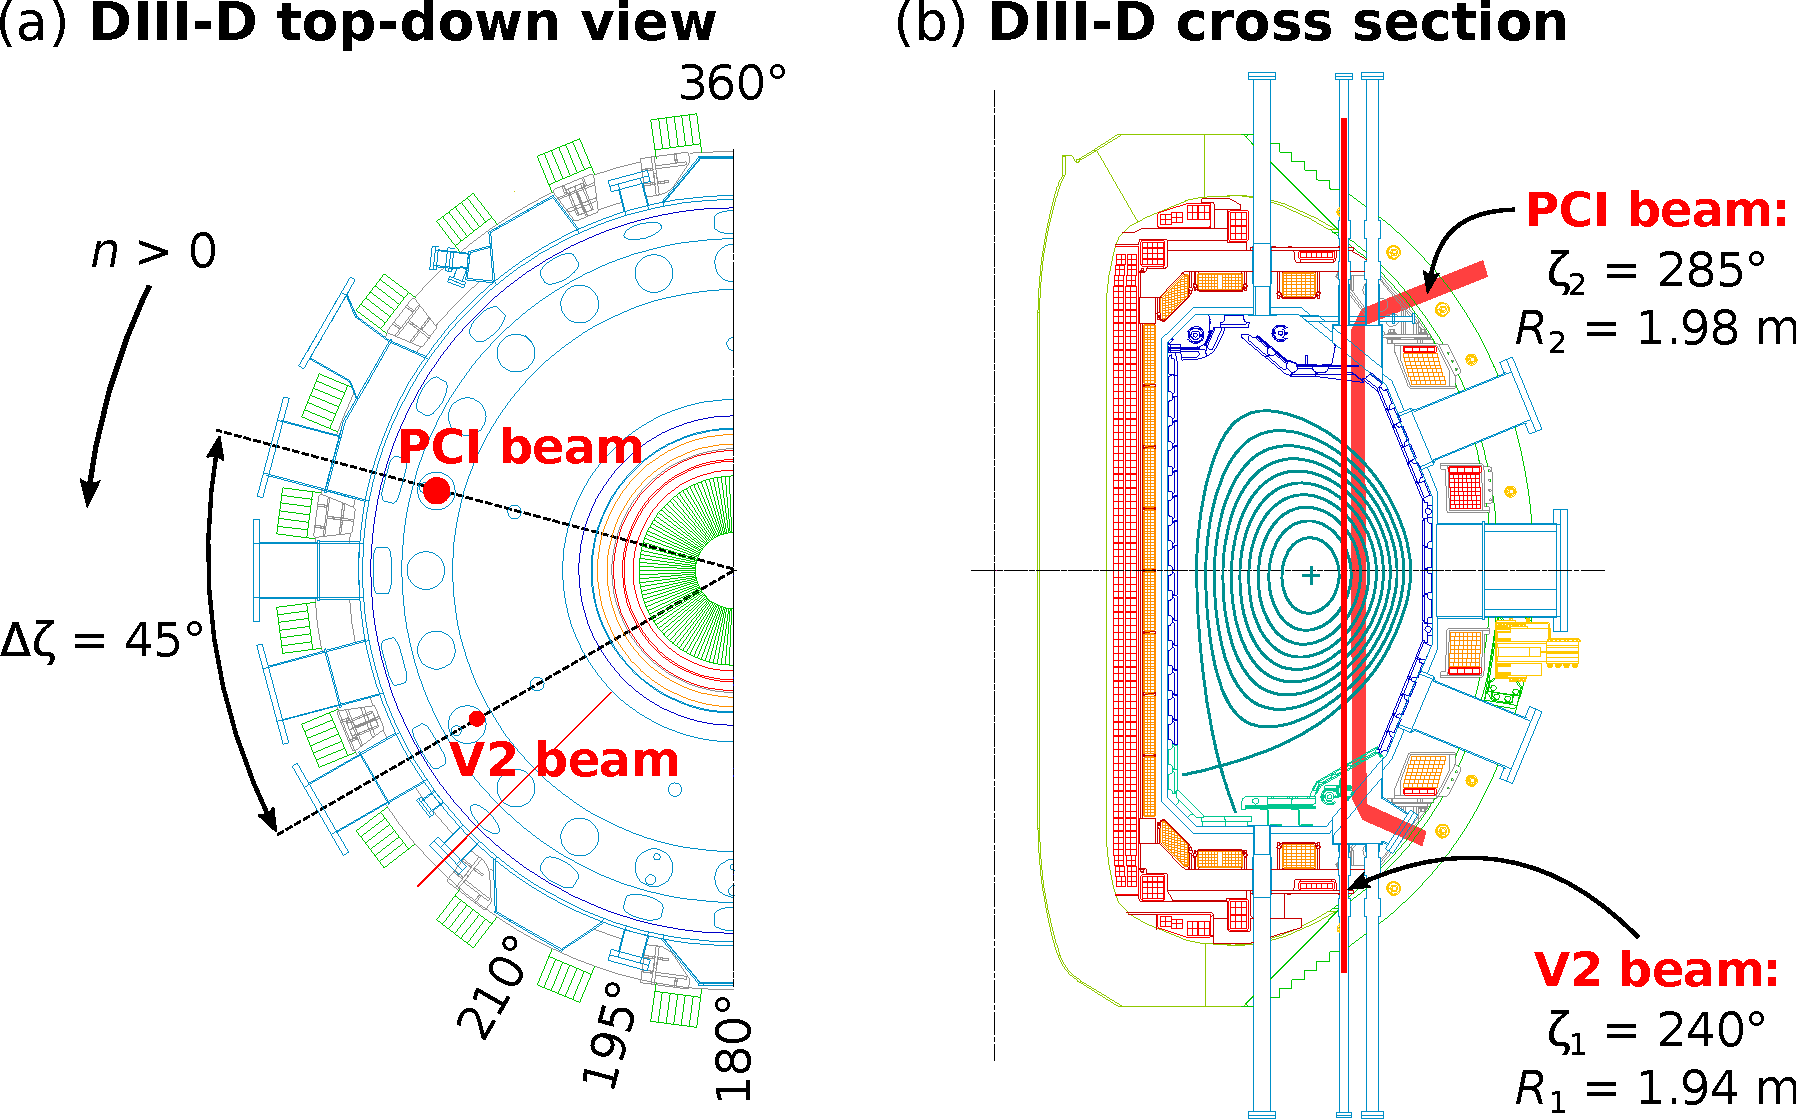
\includegraphics[width = \textwidth]{%
    Chapters/ToroidalCorrelation/figs/pci_interf_locs.pdf}
  \caption[Locations of the $V2$ and PCI interferometer beams on \diiid]{%
    (a) A top-down view of the \diiid\space vessel.
    The toroidal location of the $V2$ interferometer beam
    is $\zeta = 240^{\circ}$,
    and the toroidal location of the PCI beam
    is $\zeta = 285^{\circ}$.
    The \diiid\space sign convention for toroidal mode numbers
    is that $n > 0$ for modes that rotate counterclockwise
    when viewing the torus from above,
    as this corresponds to the direction of dominant torque injection.
    (b) A poloidal cross section of the \diiid\space vessel.
    The major-radial location of the $V2$ interferometer beam
    is $R = \SI{1.94}{\meter}$, and
    the major-radial location of the PCI beam
    is $R = \SI{1.98}{\meter}$.}
\label{fig:ToroidalCorrelation:pci_interf_locs}
\end{figure}

The addition of a heterodyne-interferometer channel
to \diiid's pre-existing phase contrast imaging (PCI) system
is discussed extensively in
Chapter~\ref{ch:Implementation} and
elsewhere~\cite{davis_rsi16}, but
the details of relevance to the toroidal-correlation measurement
are briefly reviewed here.
The PCI probe beam sits at a toroidal location of $285^{\circ}$ and
has a major-radial location $R = \SI{1.98}{\meter}$.
The location of the PCI beampath relative to that of the $V2$ interferometer
is shown in Fig.~\ref{fig:ToroidalCorrelation:pci_interf_locs}.

The geometry of the $V2$ and PCI interferometers
has consequences for the toroidal-correlation measurement.
The interferometers are
toroidally spaced by $\Delta \zeta = 45^{\circ}$
such that the Nyquist toroidal mode number
(\ref{eq:ToroidalCorrelation:Nyquist_modenumber}) becomes
\begin{equation}
  n_{\text{Ny}}
  =
  \begin{cases}
    4
    \qquad \text{for \emph{unknown} propagation direction} \\
    8
    \qquad \text{for \emph{known} propagation direction}
  \end{cases}.
  \label{eq:ToroidalCorrelation:Nyquist_modenumber_interferometers}
\end{equation}
The \diiid\space sign convention for toroidal mode numbers
is indicated in Fig.~\ref{fig:ToroidalCorrelation:pci_interf_locs};
that is, $n > 0$ for modes that rotate counterclockwise
when viewing the torus from above,
as this corresponds to the direction of dominant torque injection.
Consistency with this sign convention requires
that $x(t)$ corresponds to the $V2$ interferometer signal and
that $y(t)$ corresponds to the PCI interferometer signal
when computing the toroidal mode number via
(\ref{eq:ToroidalCorrelation:modenumber_from_cross_phase}).
Finally, the $V2$ and PCI interferometer beam paths have a slight radial offset
($\Delta R = \SI{4}{\centi\meter}$ with
$R_{\text{v2}} = \SI{1.94}{\meter}$ and
$R_{\text{pci}} = \SI{1.98}{\meter}$);
the consequences of this offset are discussed in
Section~\ref{sec:ToroidalCorrelation:ImplementationDetails:radial_offset}.

For completeness, it should also be mentioned that
a three-chord, radially viewing Faraday-effect polarimeter-interferometer
was recently installed on \diiid's $285^{\circ}$ $R0$ port~\cite{chen_rsi16}.
While diagnosing core-localized magnetic fluctuations
is the primary impetus for this installation,
the system also measures line-integrated electron-density fluctuations.
Presumably, these measurements could be correlated with those from
the $225^{\circ}$ $R0$ CO$_2$ heterodyne interferometer.
However, these two systems do not have phase-locked sampling rates
(the necessity of which is discussed in
Section~\ref{sec:ToroidalCorrelation:ImplementationDetails:phase_locked_sampling}),
so no attempts to correlate their interferometric measurements
are performed in this work.


\subsection{Interferometer-measured phase fluctuations}
\label{sec:ToroidalCorrelation:Interferometers:phase_fluctuations}
Consider a tokamak electron density fluctuation with
amplitude $\tilde{n}_0(r)$,
toroidal mode number $n$,
poloidal mode number $m$, and
angular frequency $\omega$
\begin{equation}
  \tilde{n}_e(\vect{r}, t)
  =
  \tilde{n}_0(r)
  e^{i \left(n \zeta + m \theta - \omega t \right)}.
\end{equation}
The phase fluctuation (\ref{eq:InterferometricMethods:phase_fluctuation})
imparted to a CO$_2$ probe beam
propagating \emph{vertically} through $\tilde{n}_e(\vect{r}, t)$ becomes
\begin{align}
  \tilde{\phi}
  &=
  - r_e \lambda_0 \int \tilde{n}_e(\vect{r}, t) dz.
  \notag \\
  &=
  \Phi e^{i \left( n \zeta - \omega t \right)},
  \label{eq:ToroidalCorrelation:phase_fluctuations_vertical_beam1}
\end{align}
where
\begin{equation}
  \Phi
  =
  -r_e \lambda_0
  \int \tilde{n}_0(r) e^{i m \theta} dz
  \label{eq:ToroidalCorrelation:line_integrated_radial_and_poloidal_structure}
\end{equation}
is a complex-valued function of
the beam's major-radial location and
the radial and poloidal mode structure.
For a given mode,
the $V2$ and PCI interferometers see the same
radial and poloidal mode structure such that
$\Phi$ effectively reduces to a one-dimensional function $\Phi = \Phi(R)$.
Further, $\Phi$ can be written explicitly
as a complex value $\Phi = |\Phi| e^{i \sigma}$.
Thus, the phase fluctuation
(\ref{eq:ToroidalCorrelation:phase_fluctuations_vertical_beam1})
can be written alternatively as
\begin{equation}
  \tilde{\phi}
  =
  |\Phi(R)| e^{i[n \zeta - \omega t + \sigma(R)]},
  \label{eq:ToroidalCorrelation:phase_fluctuations_vertical_beam2}
\end{equation}
where the dependence on the major radius $R$ of the beam
has been noted explicitly.


\subsection{Interferometer-measured toroidal mode number}
\label{sec:ToroidalCorrelation:Interferometers:interferometer_measured_mode_number}
Define $x(t)$ and $y(t)$ to be
the $V2$-measured and PCI-measured phase fluctuations, respectively; i.e.\
\begin{align}
  x(t)
  &=
  \tilde{\phi}_{\text{v2}}(t)
  =
  |\Phi(R_{\text{v2}})|
  e^{i[n \zeta_{\text{v2}} - \omega t + \sigma(R_{\text{v2}})]},
  \\
  y(t)
  &=
  \tilde{\phi}_{\text{pci}}(t)
  =
  |\Phi(R_{\text{pci}})|
  e^{i[n \zeta_{\text{pci}} - \omega t + \sigma(R_{\text{pci}})]}.
\end{align}
Then the cross phase (\ref{eq:ToroidalCorrelation:cross_phase}) becomes
\begin{equation}
  \alpha_{xy}
  =
  n \Delta \zeta
  +
  \left[%
    \sigma(R_{\text{pci}})
    -
    \sigma(R_{\text{v2}})
  \right],
  \label{eq:ToroidalCorrelation:interferometer_measured_cross_phase}
\end{equation}
where $\Delta \zeta = \zeta_{\text{pci}} - \zeta_{\text{v2}} = 45^{\circ}$
is the toroidal separation between the interferometer beams.
The cross phase $\alpha_{xy}$ of $x(t)$ and $y(t)$
can be readily estimated via
the non-parametric, FFT-based
spectral-estimation techniques discussed in
Appendix~\ref{app:SpectralEstimation:NonParametric}, but
$\sigma(R_{\text{pci}})$ and $\sigma(R_{\text{v2}})$
are not typically known \emph{a priori}.
Nonetheless, the measured toroidal mode number $n_{\meas}$ is defined as
\begin{equation}
  n_{\meas}
  =
  \frac{\alpha_{xy}}{\Delta \zeta},
  \qquad
  \text{where} \;\, \Delta \zeta = 45^{\circ}.
  \label{eq:ToroidalCorrelation:interferometer_measured_mode_number}
\end{equation}
However, if $\sigma(R_{\text{pci}}) \neq \sigma(R_{\text{v2}})$,
the measured mode number will not be equal to the true mode number
(i.e.\ $n_{\meas} \neq n$);
this is discussed further in
Section~\ref{sec:ToroidalCorrelation:ImplementationDetails:radial_offset}.
Further, if the true mode number exceeds the Nyquist mode number
(\ref{eq:ToroidalCorrelation:Nyquist_modenumber_interferometers}),
the measured mode number will be aliased away from the true mode number
(i.e.\ $n_{\meas} \neq n$).


% \subsection{MHD plasma-density perturbations}
% \label{sec:ToroidalCorrelation:Interferometers:MHD_theory}
% An MHD mode displaces a plasma from it's equilibrium position
% by $\vect{\xi} = \vect{\xi}(\vect{r}, t)$.
% The perturbed velocity is given as
% $\vect{v}_1 = \partial \vect{\xi} / \partial t$
% and, assuming harmonic variations, reduces to
% \begin{equation}
%   \vect{v}_1
%   \equiv
%   \frac{\partial \vect{\xi}}{\partial t}
%   =
%   -i \omega \vect{\xi},
%   \notag
% \end{equation}
% where $\omega$ is the mode's angular frequency.
% The plasma density $n_i$ is given as
% \begin{equation}
%   n_i = \bar{n}_i + \tilde{n}_i,
%   \notag
% \end{equation}
% where $\bar{n}_i$ and $\tilde{n}_i$ are
% the equilibrium and fluctuating components, respectively.
% Assuming a stationary equilibrium ($\vect{v}_0 = 0$) and
% using the above relations,
% the linearized continuity equation reduces to
% \begin{equation}
%   \tilde{n}_i = -\nabla \cdot (\bar{n}_i \vect{\xi}).
%   \label{eq:ToroidalCorrelation:density_fluctuations}
% \end{equation}
% If we relax the assumption on $\vect{v}_0$ to allow
% finite equilibrium flow ($\vect{v}_0 \neq 0$),
% then the right-hand side of (\ref{eq:ToroidalCorrelation:density_fluctuations})
% is simply multiplied by the prefactor
% $[1
% - (\vect{v}_0 \cdot \vect{k} / \omega)
% + i (\nabla \cdot \vect{v}_0 / \omega)]^{-1}$, where
% $\vect{k}$ is the mode wavevector.


\section{Implementation details and non-ideal effects}
\label{sec:ToroidalCorrelation:ImplementationDetails}
This section discusses various implementation details and non-ideal effects
regarding the toroidal correlation of the $V2$ and PCI interferometers.
Specifically, Section~\ref{sec:ToroidalCorrelation:ImplementationDetails:phase_locked_sampling}
describes the modifications to the $V2$ and PCI digitizers
that now enable phase-locked measurements.
Section~\ref{sec:ToroidalCorrelation:ImplementationDetails:trigger_offset}
unveils the presence of a deleterious ``trigger offset''
between the phase-locked systems but
also demonstrates an easy and robust methodology
for estimating and compensating this offset
in post-processing software.
Section~\ref{sec:ToroidalCorrelation:ImplementationDetails:validation_agains_magnetics}
then compares the interferometer-measured toroidal mode numbers
with those measured by \diiid's array of midplane magnetic probes,
typically resulting in good agreement for large, robust tearing modes.
Finally, Section~\ref{sec:ToroidalCorrelation:ImplementationDetails:radial_offset}
discusses how the $\Delta R = \SI{4}{\centi\meter}$ major-radial offset
between the $V2$ and PCI interferometers
can bias the measured toroidal mode numbers;
eliminating this radial offset is not possible
with the current port allocations, but
future work to empirically or computationally account
for the radial and poloidal mode structures
may aid the interpretation
of the interferometer-measured toroidal mode numbers.


\subsection{Phase-locked sampling}
\label{sec:ToroidalCorrelation:ImplementationDetails:phase_locked_sampling}
Extracting useful information
from the correlation of two measurements
requires that the sampling rates of the two measurements
are \emph{phase-locked}.
If the sampling rates are \emph{not} phase-locked,
slippage between the sampling times
will result in artificial evolution of the measured phase.

Digitizing the two signals on a common digitizer
is the simplest method for ensuring phase-locked sampling.
Unfortunately, such an approach is not suitable
for the $V2$ and PCI interferometer signals.
The $V2$ interferometer's
$\Delta f_0 = \SI{40}{\mega\hertz}$ intermediate-frequency signal
is demodulated using an all-digital technique
that mandates use of a sampling rate
$f_s = (4 / 3) \Delta f_0$
\cite{vanzeeland_rsi08}, and
the baseband $I$ and $Q$ signals never exist in analog form.
In contrast, as described in
Chapter~\ref{ch:Implementation} and \cite{davis_rsi16},
the PCI interferometer's
$\Delta f_0 = \SI{30}{\mega\hertz}$ intermediate-frequency signal
is demodulated with analog electronics, and
the analog baseband $I$ and $Q$ signals
are then digitized on two channels of a D-tAcq ACQ$216$ CPCI board.
Because the $V2$ interferometer's baseband $I$ and $Q$ signals
never exist in analog form,
it is not possible to digitize the $V2$ $I$ and $Q$ signals
on the digitizer used by the PCI interferometer.
Further, because of the intermediate-frequency mismatch
between the $V2$ and PCI interferometers,
it is also not possible digitally demodulate and digitize
the PCI interferometer's $\SI{30}{\mega\hertz}$ intermediate-frequency signal
using the $V2$ interferometer's
$\SI{40}{\mega\hertz}$ digital demodulation system.
An alternative approach is to directly digitize
both intermediate-frequency signals
with a high-bandwidth digitizer and
demodulate both signals in software,
as has been done elsewhere~\cite{mlynek_fst12}.
While \diiid's ion cyclotron emission (ICE) digitizer
has a $200 \, \text{MSPS}$ sample rate,
channels on the ICE digitizer are not consistently available.

As sharing a common digitizer is not possible,
phase-locked sampling between the $V2$ and PCI interferometers
requires that the digitizers of both systems
derive their clocks from a common source.
The $V2$ interferometer derives its clock
from a $\SI{320}{\mega\hertz}$ oven-controlled crystal oscillator (OCXO), and
its digital demodulation system
has two auxiliary outputs that can be programmed
to output phase-locked LVCMOS signals
at $\SI{320}{\mega\hertz} / N$, where
$N \in \{1, 2, 3, ..., 32\}$.
Both outputs are currently programmed with divisor $N = 20$
such that they each provide a $\SI{16}{\mega\hertz}$ clock signal.
One of these $\SI{16}{\mega\hertz}$ clock signals
is routed via an RG-$58$ coaxial cable
from the $V2$ digital demodulation hardware
in the first row of the \diiid\space annex
to the PCI digitizer
in the third row of the \diiid\space annex.

The PCI digitizer typically samples at $f_s = 4 \, \text{MSPS}$.
Thus, division of the $V2$ $\SI{16}{\mega\hertz}$ clock by four
(in hardware or software) yields a clock appropriate for typical sampling.
Each board of the PCI digitizer can accept an external clock
through the front panel's single-pin LEMO CLK input.
The CLK signal passes through an optocoupler
with a bandwidth $\sim \SI{10}{\mega\hertz}$
\cite{milne_optocoupler_pc16}, but
in-house tests have demonstrated
that the input clock frequency
can actually exceed $\SI{16}{\mega\hertz}$.
As a result, the $\SI{16}{\mega\hertz}$ signal
is directly connected to the front-panel LEMO CLK input
of the ``master'' digitizer board (``board $8$''), and
the necessary division
(i.e.\ divide by four to achieve typical $4 \, \text{MSPS}$ sampling rate)
is performed within the digitizer board,
which is cleaner, simpler, and more easily extensible
than performing the division in hardware.
The resulting $\SI{4}{\mega\hertz}$ clock
is routed to the ``slave'' digitizer board (``board $7$'')
via the PXI backplane.
The phase-locked sampling of the $V2$ and PCI systems
has been in place since June 2016.


\subsection{Estimating \& compensating the ``trigger offset''}
\label{sec:ToroidalCorrelation:ImplementationDetails:trigger_offset}
As discussed in Appendix~\ref{app:DigitizerSynchronization},
phase-locked digitizers can still suffer from
a so-called ``trigger offset'', as defined by
(\ref{eq:DigitizerSynchronization:trigger_offset}).
A finite trigger offset results
(a) when a digitizer triggers at a time $\delta t$ later
than its nominal trigger time and
(b) when the sampling rate deviates from the nominal sampling rate
and the nominal trigger times of both digitizers differ.

\begin{figure}
  \centering
  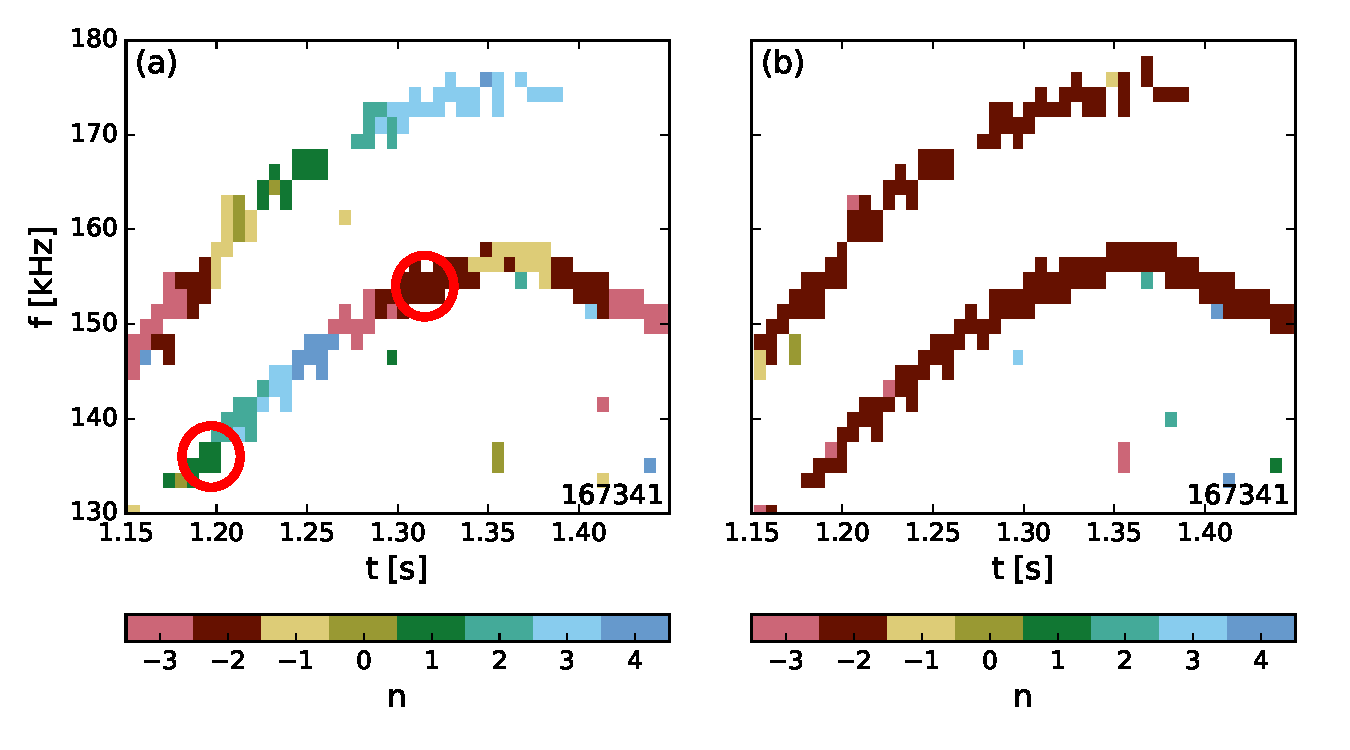
\includegraphics[width = \textwidth]{%
    Chapters/ToroidalCorrelation/figs/trigger_offset.pdf}
  \caption[``Trigger offset'' compensation]{%
    Interferometer-measured toroidal mode numbers
    (a) \emph{without} compensation for the trigger offset and
    (b) \emph{with} compensation for the trigger offset.
    In (a), the finite trigger offset
    (\ref{eq:ToroidalCorrelation:trigger_offset_optimized})
    results in the unphysical evolution
    of the measured toroidal mode numbers.
    The trigger offset is roughly estimated
    from the measured mode-number evolution
    between the red circular annotations
    to the lower-frequency mode
    ($\Delta f \approx \SI{20}{\kilo\hertz}$ and
    $\Delta n \approx 5$; note that $\Delta n_{\meas}$
    refers to the total number of mode numbers evolved through,
    i.e.\ it is path-dependent and is \emph{not} simply
    the difference between the final and initial $n_{\meas}$).
    In (b), the digital records of both interferometers
    have been synchronized by compensating for the finite trigger offset
    (\ref{eq:ToroidalCorrelation:trigger_offset_optimized}), and
    the measured toroidal mode numbers are constant in time,
    consistent with physical expectations.
    The $6$-digit number in the upper right-hand corner
    indicates the \diiid\space shot.
  }
\label{fig:ToroidalCorrelation:trigger_offset}
\end{figure}

A finite trigger offset biases mode-number measurements.
For example, Fig.~\ref{fig:ToroidalCorrelation:trigger_offset}(a)
displays the toroidal mode numbers of two coherent modes
as measured by the uncompensated interferometers.
Note that the measured mode number of each mode
(unphysically) evolves with the mode frequency,
which is consistent
(see (\ref{eq:DigitizerSynchronization:measured_phase_difference}))
with the presence of a finite trigger offset
between the interferometer measurements.
Referencing
(\ref{eq:DigitizerSynchronization:trigger_offset_estimate_frequency_swept}),
the trigger offset can be estimated
from the measured mode-number evolution
during a linear frequency sweep as
\begin{align}
  \delta t_{\trig}
  =
  \frac{d \alpha_{xy}}{d\omega}
  \approx
  \frac{\Delta \alpha_{xy}}{\Delta \omega}
  \approx
  \SI{30}{\micro\second},
\end{align}
where
$\Delta \alpha_{xy} = \Delta \zeta \cdot \Delta n_{\meas}$
is the measured phase-angle change and
$\Delta \zeta = \pi / 4$
is the angular separation of the interferometers
(consistent with
(\ref{eq:ToroidalCorrelation:interferometer_measured_mode_number}));
here, the numerical value results from
$\Delta n_{\meas} \approx 5$ and
$\Delta \omega \approx 2 \pi \cdot \SI{20}{\kilo\hertz}$,
as indicated by the red circular annotations
to the lower-frequency mode in
Fig.~\ref{fig:ToroidalCorrelation:trigger_offset}(a).
Note that $\delta t_{\trig} > 0$
implies that the actual sampling times
of the PCI interferometer lag (i.e.\ occur later than)
those of the $V2$ interferometer, as shown schematically in
Fig.~\ref{fig:DigitizerSynchronization:trigger_offset_schematic}.
Applying standard techniques~\cite[Sec.~4.5]{oppenheim}
in post-processing software
to eliminate this $\SI{30}{\micro\second}$ timebase discrepancy
dramatically reduces the unphysical mode-number evolution observed in
Fig.~\ref{fig:ToroidalCorrelation:trigger_offset}(a).
Scanning $\delta t_{\trig}$ about $\SI{30}{\micro\second}$
shows that the unphysical mode-number evolution is minimized for
\begin{equation}
  \delta t_{\trig}
  =
  \SI{32.5}{\micro\second}.
  \label{eq:ToroidalCorrelation:trigger_offset_optimized}
\end{equation}
Fig.~\ref{fig:ToroidalCorrelation:trigger_offset}(b)
displays the interferometer-measured toroidal mode numbers
after compensating for trigger offset
(\ref{eq:ToroidalCorrelation:trigger_offset_optimized});
note that the mode numbers are constant in time,
consistent with physical expectations.
It should be emphasized that the only difference between
Fig.~\ref{fig:ToroidalCorrelation:trigger_offset}(a) and
Fig.~\ref{fig:ToroidalCorrelation:trigger_offset}(b)
is the compensation of trigger offset
(\ref{eq:ToroidalCorrelation:trigger_offset_optimized}).

Trigger offset (\ref{eq:ToroidalCorrelation:trigger_offset_optimized})
has been robustly stable
since phase-locking the $V2$ and PCI digitizers in June 2016,
a timescale currently exceeding one year.
It is interesting to examine the physical origin
of this trigger offset to understand when it might change.
Referencing the definition of $\delta t_{\trig}$ in
(\ref{eq:DigitizerSynchronization:trigger_offset}),
there are three distinct mechanisms contributing to the trigger offset.
The first effect is the difference
between the trigger-time discrepancies $\delta t_j$ of each digitizer;
in a properly functioning digitizer,
this is discrepancy is typically smaller than one or two sample times
(i.e.\ $\lesssim \SI{1}{\micro\second}$ for the digitizers considered here),
making it an unlikely source of the relatively large trigger offset
(\ref{eq:ToroidalCorrelation:trigger_offset_optimized}).
The second effect is
the digitizers' normalized sampling-rate deviation $\bar{\delta F_j}$
(phase-locked digitizers have \emph{equal}
normalized sampling-rate deviations;
see (\ref{eq:DigitizerSynchronization:phase_locked_normalized_sample_rate_deviations})).
Because the trigger offset
(\ref{eq:ToroidalCorrelation:trigger_offset_optimized})
does \emph{not} appear to vary in time,
temporal fluctuations in $\bar{\delta F_j}$ cannot be responsible;
however, $\bar{\delta F_j}$ will be constant and finite
if the sampling rate has a constant offset
from the nominal sampling rate.
The third effect is the weighting of $\bar{\delta F_j}$
by the difference in nominal trigger times.
Now, the $V2$ digitizer nominally triggers at
$t_{\text{v2}}^{\nom}[0] \approx \SI{-1.5}{\second}$
relative to plasma breakdown, while
the PCI digitizer nominally triggers at
$t_{\text{pci}}^{\nom}[0] = \SI{-0.05}{\second}$
relative to plasma breakdown.
Solving for the $\bar{\delta F_j}$ in
(\ref{eq:DigitizerSynchronization:trigger_offset}) and
neglecting the small trigger-time discrepancies $\delta t_j$ yields
\begin{equation}
  \bar{\delta F_j}
  \approx
  \frac{\delta t_{\trig}}{t_{\text{pci}}^{\nom}[0] - t_{\text{v2}}^{\nom}[0]}
  \approx
  2.2 \times 10^{-5},
\end{equation}
which is not an unreasonable precision
for the digitizer sampling rates.
Thus, digitizer offset
(\ref{eq:ToroidalCorrelation:trigger_offset_optimized})
appears to result from the combined effects of
finite sampling-rate precision (i.e.\ nonzero $\bar{\delta F_j}$) and
the difference between the nominal trigger times
of the $V2$ and PCI digitizers.
Importantly, if the nominal trigger times of
the $V2$ or PCI digitizers are altered in the future,
the trigger offset will also change and
will need to be estimated from new measurements.


\subsection{Validation against magnetic measurements}
\label{sec:ToroidalCorrelation:ImplementationDetails:validation_agains_magnetics}
\begin{figure}
  \centering
  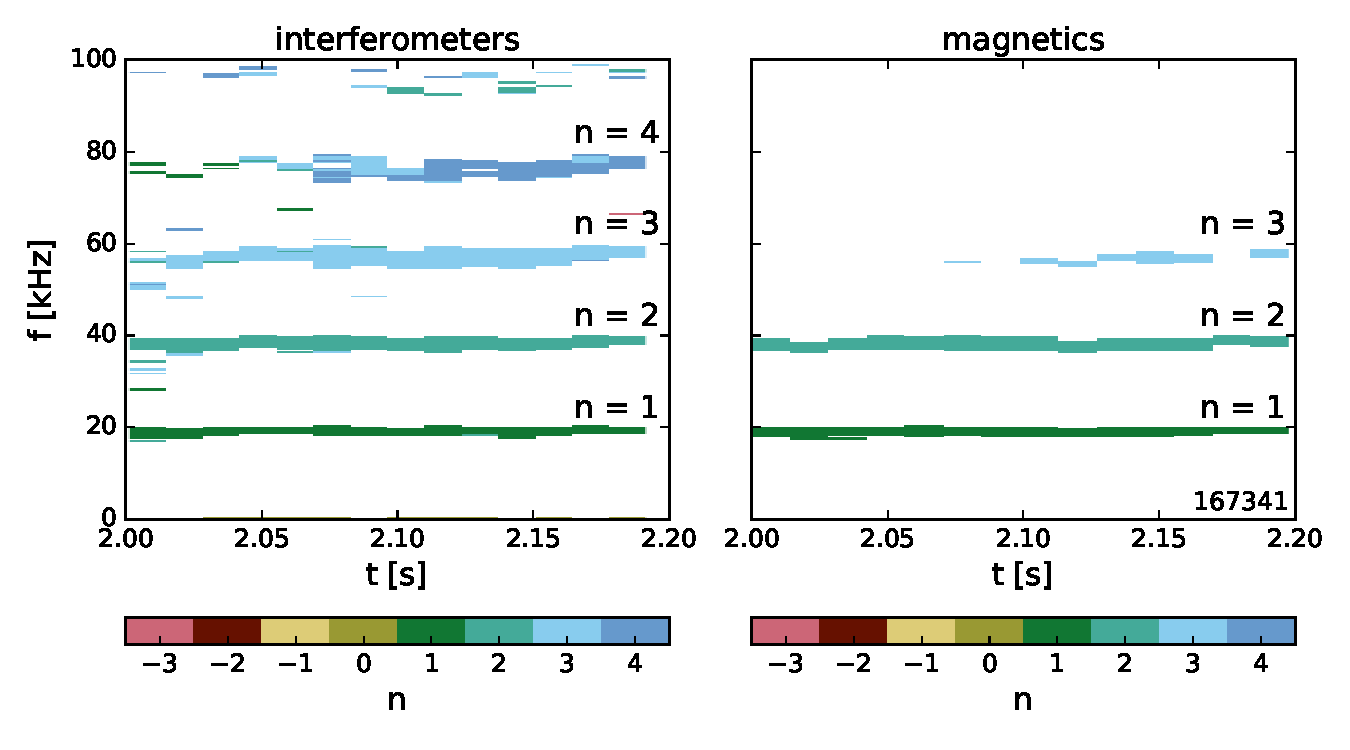
\includegraphics[width = \textwidth]{%
    Chapters/ToroidalCorrelation/figs/magnetics_comparison.pdf}
  \caption[Interferometric \& magnetic measurement of toroidal mode numbers]{%
    A comparison of interferometric (left) and magnetic (right)
    measurements of toroidal mode numbers.
    Here, cross-spectral densities are estimated
    by averaging over $\approx \SI{14}{\milli\second}$ ``ensembles'',
    each of which consists of $10$ ``realizations'';
    adjacent realizations have $50\%$ overlap, and
    a Hanning window is applied to each realization
    prior to performing any spectral computations.
    Only points with magnitude-squared coherence
    $\gamma_{xy}^2 \geq 0.5$ are displayed
    in the interferometer spectrum, while
    only points with coefficient of determination
    $R^2 \geq 0.9$ are displayed
    in the magnetic spectrum.
    See Appendix~\ref{app:SpectralEstimation}
    for background regarding spectral estimation.
    The $6$-digit number in the lower right-hand corner
    indicates the \diiid\space shot.
  }
\label{fig:ToroidalCorrelation:magnetics_comparison}
\end{figure}

After compensating for the trigger offset
(\ref{eq:ToroidalCorrelation:trigger_offset_optimized}),
the interferometer-measured toroidal mode numbers can be validated against
those measured by the \diiid\space midplane magnetic probes
\cite{strait_rsi06}.
The magnetic probes measure the
poloidal magnetic-field perturbation $\tilde{B}_{\theta}$,
as eddy currents in the wall tend to reinforce $\tilde{B}_{\theta}$
(in contrast, eddy currents tend to shield
the radial perturbations $\tilde{B}_{r}$).
While toroidal mode numbers can be computed
via two-point correlation of a single magnetic-probe pair,
a more robust estimate can be made
by correlating each unique magnetic-probe pair and
then least-squares fitting
the resulting cross-phase estimates vs.\
the corresponding toroidal separations to a linear model;
all of the magnetics-measured toroidal mode numbers
presented in this work
are computed via this more robust estimation method.
Fig.~\ref{fig:ToroidalCorrelation:magnetics_comparison}
compares the interferometer-measured and the magnetics-measured
toroidal mode numbers;
both measurements indicate the presence of an $n = 1$ tearing mode and
several higher order harmonics.
The good agreement between the interferometric and magnetic measurements
is typical for large, robust tearing modes.


\subsection{Effect of major-radial offset}
\label{sec:ToroidalCorrelation:ImplementationDetails:radial_offset}
As discussed in Section~\ref{sec:ToroidalCorrelation:Interferometers:diiid},
the beams of the $V2$ and PCI interferometers have a
$\Delta R = \SI{4}{\centi\meter}$ major-radial offset.
This major-radial offset can bias the measured cross phase
(\ref{eq:ToroidalCorrelation:interferometer_measured_cross_phase})
between the two interferometer signals,
which produces a corresponding bias
in the interferometer-measured toroidal mode number
(\ref{eq:ToroidalCorrelation:interferometer_measured_mode_number}).
The cross-phase bias in
(\ref{eq:ToroidalCorrelation:interferometer_measured_cross_phase})
is $\sigma(R_{\text{pci}}) - \sigma(R_{\text{v2}})$, where
$\sigma(R) = \arg[\Phi(R)]$ and $\Phi(R)$ is proportional to
the line-integrated radial and poloidal mode structure
at major radius $R$, as defined in
(\ref{eq:ToroidalCorrelation:line_integrated_radial_and_poloidal_structure}).
Now, if the mode structure is up-down symmetric about the midplane,
$\Phi$ is real, and
$\sigma(R_{\text{pci}}) - \sigma(R_{\text{v2}}) \in \{0, \pi\}$.
The toroidal mode number is correctly identified
when $\sigma(R_{\text{pci}}) - \sigma(R_{\text{v2}}) = 0$ but
is aliased (and thus incorrectly identified)
when $\sigma(R_{\text{pci}}) - \sigma(R_{\text{v2}}) = \pi$.
If the radial mode structure evolves such that
$\sigma(R_{\text{pci}}) - \sigma(R_{\text{v2}}) = 0 \rightarrow \pi$
or vice versa,
the measured mode number will ``jump'';
an example of such mode-number ``jumping'' is shown in
Fig.~\ref{fig:ToroidalCorrelation:mode_number_jumps}.
If the mode structure is up-down asymmetric about the midplane, however,
$\Phi$ is complex, and
the bias to the measured mode number becomes continuous, rather than discrete.
Fast-ion shearing of Alfv\'{e}n eigenmodes~\cite{tobias_prl11},
for example, produces such up-down asymmetries.

\begin{figure}
  \centering
  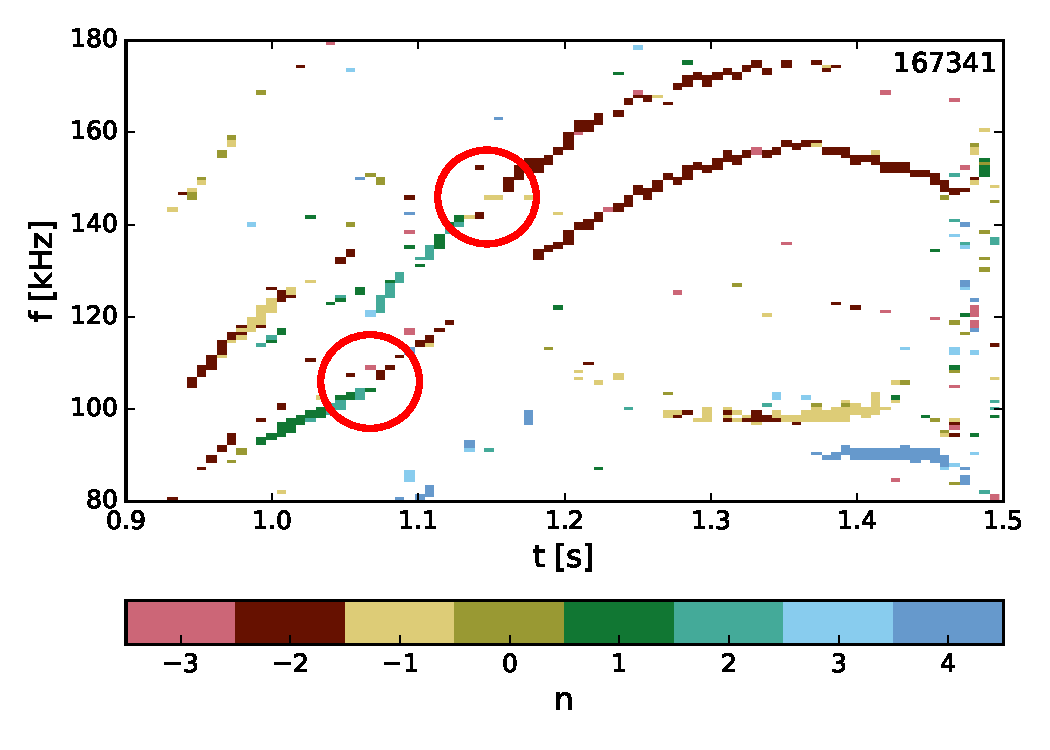
\includegraphics[width = 0.85 \textwidth]{%
    Chapters/ToroidalCorrelation/figs/mode_number_jumps.pdf}
  \caption[Mode-number ``jumping'' due to major-radial offset of interferometers]{%
    When the radial mode structure evolves,
    the $\Delta R = \SI{4}{\centi\meter}$ major-radial offset
    between the $V2$ and PCI interferometers can produce
    unphysical ``jumping'' of the measured toroidal mode number,
    indicated here with red circular annotations.
    The $6$-digit number in the upper right-hand corner
    indicates the \diiid\space shot.
  }
\label{fig:ToroidalCorrelation:mode_number_jumps}
\end{figure}

Unfortunately, there is not currently a tested, robust method
for correcting the bias introduced by
the major-radial offset of the interferometers
(other than reducing the offset, i.e.\ $\Delta R \rightarrow 0$,
which is not possible with current port allocations).
Although external magnetic probes can corroborate
the interferometer-measured mode numbers in some cases,
such as in Fig.~\ref{fig:ToroidalCorrelation:magnetics_comparison},
they are blind to core-localized fluctuations.
It may be possible to account for the radial and poloidal mode structure
via measurements from
microwave imaging reflectometry (MIR)~\cite{muscatello_rsi14} or
electron cyclotron emission imaging (ECEI)~\cite{tobias_rsi10}
or via predictions from
ideal MHD (e.g.\ NOVA~\cite{cheng_jcp87, cheng_pr92})
or hybrid MHD-gyrofluid (e.g.\ TAEFL~\cite{spong_pfb92, spong_ps92}) codes,
but such efforts were deemed beyond the scope of this work.
If future modeling work is conducted to aid the interpretation
of the interferometer-measured toroidal mode numbers,
note that ideal MHD cannot capture the empirically relevant
fast-ion shearing of Alfv\'{e}n eigenmodes~\cite{tobias_prl11}.


\section{Diagnosis of core-localized MHD}
\label{sec:ToroidalCorrelation:CoreLocalized}
Directly measuring the toroidal mode numbers of core-localized MHD
was one of the primary motivations for the addition
of a heterodyne-interferometer channel to \diiid's pre-existing PCI system.
As discussed in
Section~\ref{sec:ToroidalCorrelation:ImplementationDetails:radial_offset},
however, the $\Delta R = \SI{4}{\centi\meter}$ major-radial offset
between the $V2$ and PCI beams
introduces ambiguities in the interferometer-measured mode numbers.
Further, because core-localized MHD is, by definition,
invisible to external magnetic probes,
the interferometer-measured mode numbers
cannot be corroborated by magnetics.
Although the interferometer-measured mode numbers
may currently be biased away from their true values,
the mere presence of core-localized MHD in the interferometer signals
should still be considered an encouraging proof of principle,
where future work to eliminate the major-radial offset
would allow direct and accurate
mode-number measurements of core-localized MHD.

Fig.~\ref{fig:ToroidalCorrelation:core_localized}
provides such a proof of principle.
The top panel displays the fluctuating poloidal magnetic-field spectrum
measured by a high-frequency magnetic probe~\cite{strait_rsi06}, while
the second panel displays the toroidal mode numbers
measured by the midplane array
of lower-bandwidth magnetic probes~\cite{strait_rsi06}.
The third panel shows the interferometer-measured toroidal mode numbers,
indicating very good agreement with the low-bandwidth magnetic measurements;
however, between $\SI{1.8}{\second}$ and $\SI{2.2}{\second}$,
the interferometers measure a burst of fluctuations
that are invisible to the low- and high-bandwidth magnetic probes,
indicating that the modes are core-localized.
The modes are triggered when
the on-axis safety factor $q_0$ drops below unity.
Unfortunately, additional observations of core-localized MHD
proved to be surprisingly rare, and
no systematic behavior could be identified
linking the few-and-far-between occurrences.

\begin{figure}
  \centering
  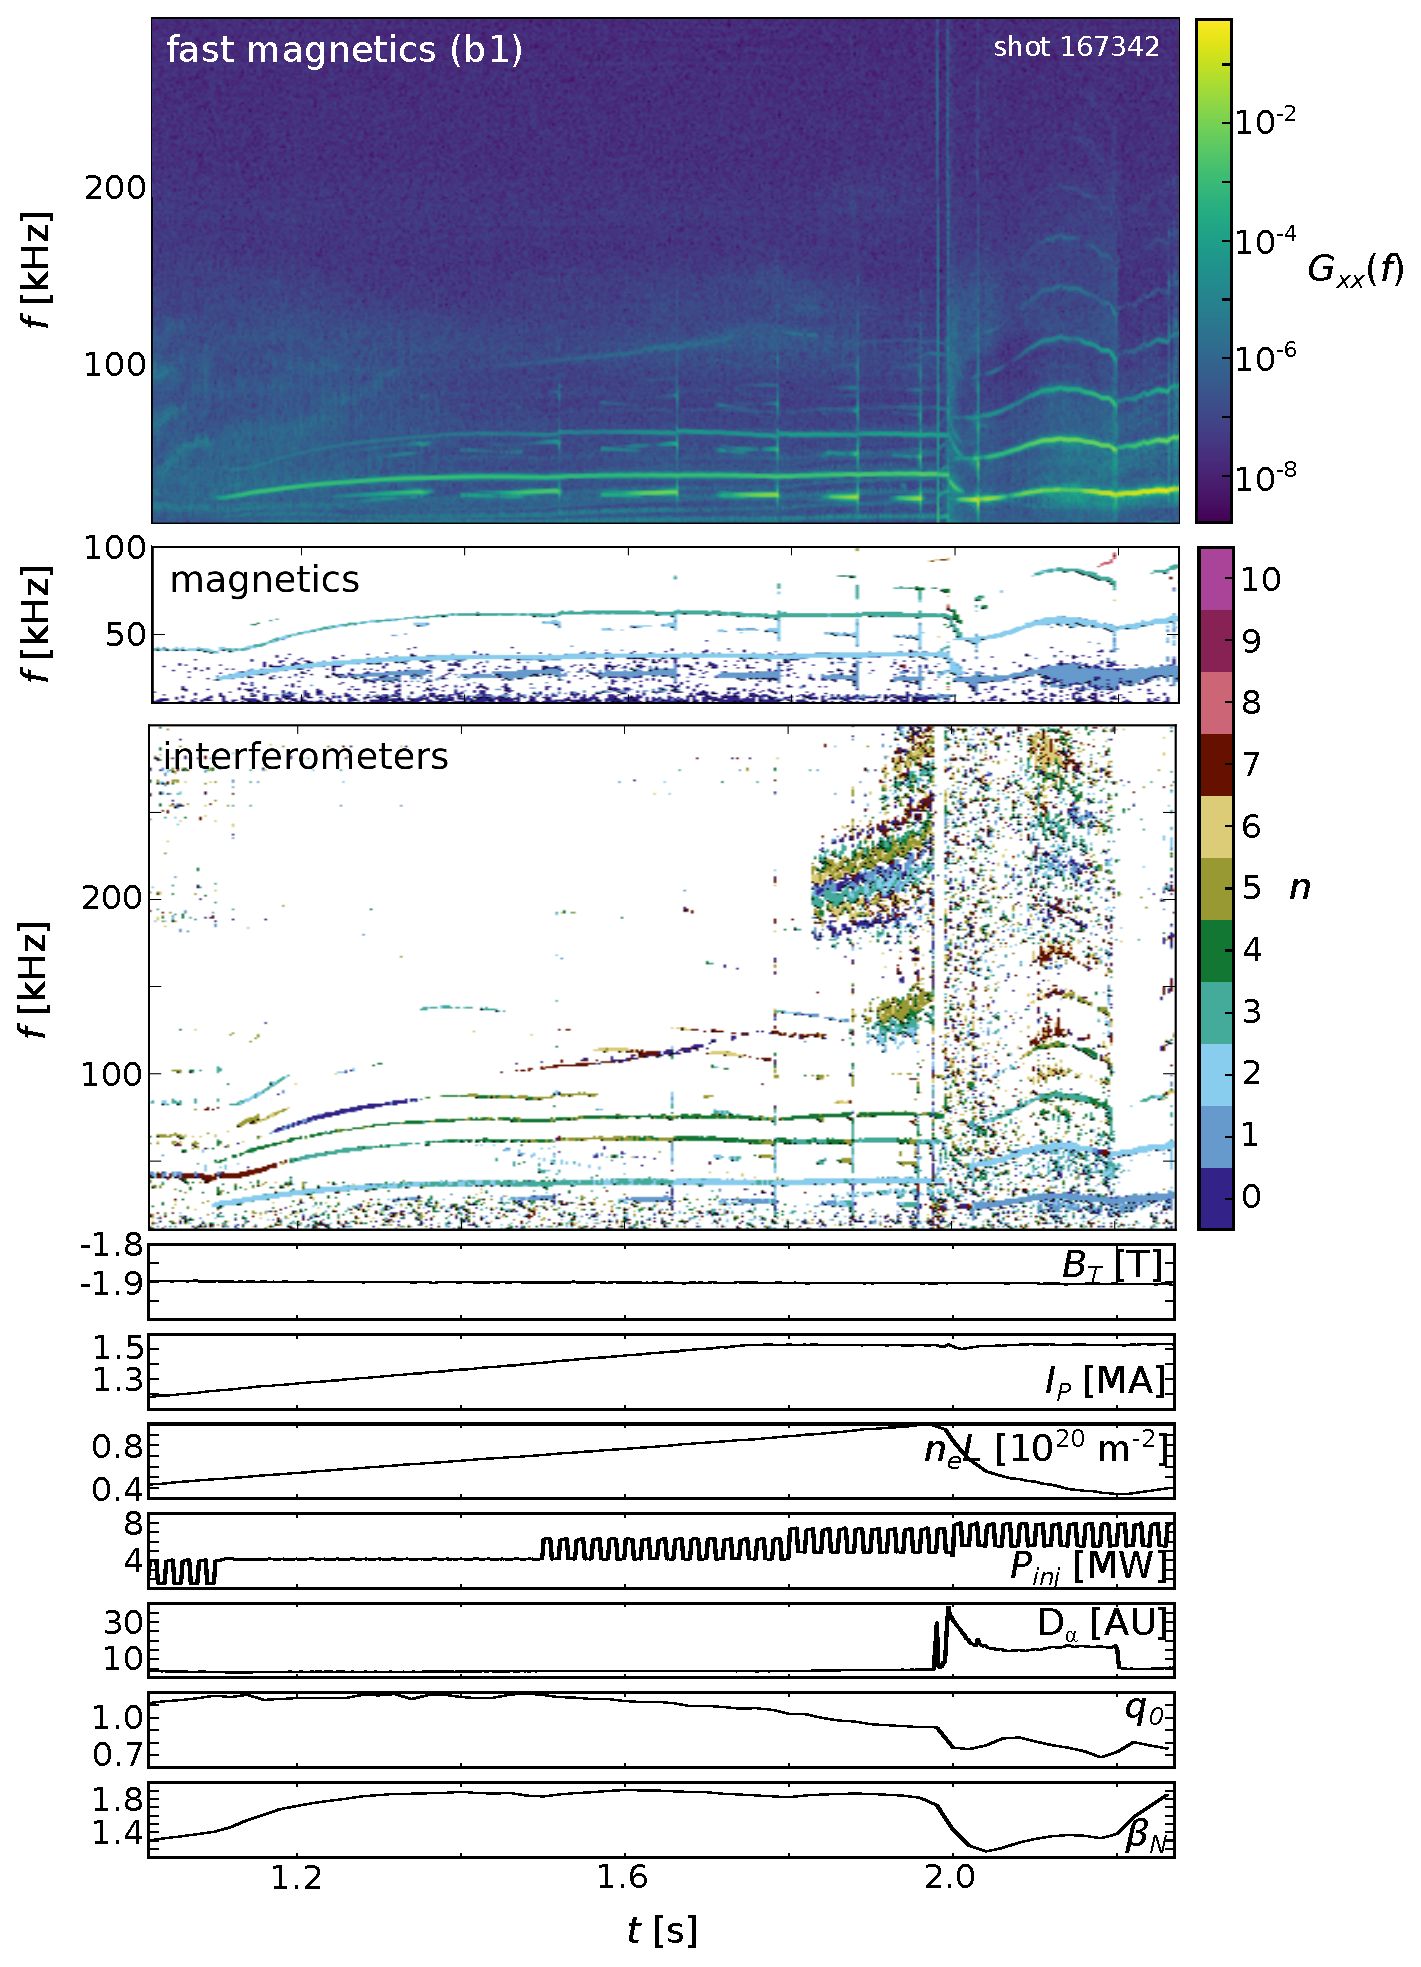
\includegraphics[width = \textwidth]{%
    Chapters/ToroidalCorrelation/figs/core_localized_167342.eps}
  \caption[Toroidal mode numbers of \emph{core-localized} MHD]{%
    Between $\SI{1.8}{\second}$ and $\SI{2.2}{\second}$,
    the correlated interferometers ($3\ts{rd}$ panel) measure
    a burst of fluctuations that are
    \emph{invisible} to magnetics ($1\ts{st}$ and $2\ts{nd}$ panels).
    This suggests that the modes are \emph{core-localized} and
    that the correlated interferometers are indeed capable
    of measuring core-localized MHD.
    Various plasma parameters of interest are shown in the lower panels;
    the modes are triggered when
    the on-axis safety factor $q_0$ drops below unity.
  }
\label{fig:ToroidalCorrelation:core_localized}
\end{figure}


\bibliographystyle{plainurl}
\bibliography{references}
%
\chapter{Multiscale turbulence measurements}
\label{ch:TurbulenceMeasurements}
The development of a first-principles understanding
of turbulent transport in a tokamak
is a long-standing goal of the fusion community.
Such a model would allow accurate design and optimization of a tokamak.
Before such a model is accepted, however,
it must be validated against experimental measurements.
Ideally, this validation should be multi-tiered,
with the model accurately and robustly reproducing
experimental observations at all scales,
from macroscopic parameters such as the turbulent heat flux to
the details of the turbulent spectrum
(e.g.\ power spectral densities, cross phases, nonlinear couplings, etc.).

Along these lines,
this chapter presents measurements of electron-density turbulence
made over a wide spatiotemporal bandwidth
during a recent \diiid\space experiment.
Section~\ref{sec:TurbulenceMeasurements:Background}
begins with a brief overview of the drift-wave turbulence
often observed in tokamak plasmas,
emphasizing recent results
from realistic multiscale simulations
\cite{howard_pp14, howard_nf16, howard_pp16, howard_ppcf18, holland_nf17}.
Section~\ref{sec:TurbulenceMeasurements:ExperimentalConditions}
then describes the recent \diiid\space experiment,
which was designed to probe the multiscale nature
of plasma turbulence.
As such, this experiment presents an ideal opportunity
for multiscale turbulence investigations
with the combined PCI-interferometer.
Next, Section~\ref{sec:TurbulenceMeasurements:Measurements}
details the measurements from the combined PCI-interferometer.
Numerous turbulent branches are observed.
In particular, the interferometer measures
a low-$k$ electromagnetic mode driven unstable by collisionality,
properties consistent with the micro-tearing mode (MTM), and
the PCI measures a wavenumber spectrum
that exhibits distinct flattening
when increasing the electron-scale turbulent drive
relative to the ion-scale turbulent drive,
reminiscent of results
from realistic multiscale gyrokinetic simulations~\cite{howard_pp16}.
Finally, to aid the interpretation of these measurements,
linear-stability analysis and quasilinear-transport modeling
are performed with the TGLF code
in Section~\ref{sec:TurbulenceMeasurements:Modeling}, and
qualitative agreement with the PCI-measured wavenumber spectrum
is obtained.


\section{Overview of drift-wave turbulence}
\label{sec:TurbulenceMeasurements:Background}
The radial transport of particles, heat, and momentum in a tokamak plasma is
often larger than that predicted by collisional (i.e.\ neoclassical) theory.
There is strong theoretical and experimental evidence
that this ``anomalous'' transport
results from drift-wave turbulence
driven by the free energy in the plasma gradients
\cite{horton_drift_waves,tynan_ppcf09}.
This turbulence can be characterized by
its driving gradients,
its spatiotemporal characteristics,
the role of trapped particles, and
whether or not it is electrostatic
(as opposed to electromagnetic).

The plasma gradients are often quantified in terms of scale lengths.
The scale length of quantity $x$ is defined as
$L_x = x / \nabla x = (\nabla \ln x)^{-1}$.
Smaller values of $|L_x|$ indicate
more rapid spatial variation
(i.e.\ steeper gradient) of quantity $x$.
Thus, the free energy in profile $x$ increases with
the inverse scale length $1 / L_x$.
For theoretical analysis,
it is conventional to normalize $L_x$
to a relevant length in the system under study;
below, scale lengths are normalized
to the tokamak minor radius $a$,
which is appropriate for studies of radial transport.
Thus, the drive for instability is quantified
by the normalized inverse scale length $a / L_x$.
The ratio of density scale length to temperature scale length
$\eta_j = L_{n_j} / L_{T_j}$ for species $j$
is an additional dimensionless parameter
that is often used for instability characterization.

Due to the relatively large size of its eddies,
ion-scale ($k_{\theta} \rho_s < 1$) turbulence is often considered
to be the most detrimental to confinement.
Here, $k_{\theta}$ is a typical poloidal wavenumber of the turbulent mode,
$\rho_s = c_s / \Omega_i$ is the ion gyroradius
evaluated at the ion sound speed,
$c_s = (T_e / m_i)^{1/2}$ is the ion sound speed, and
$\Omega_i = e B / m_i$ is the ion angular cyclotron frequency.
The temporal ordering of ion-scale turbulence is usually expressed as
$k_{||} \text{v}_{ti} \ll \omega \ll k_{||} \text{v}_{te}$
\cite[Sec.~8.3]{wesson},
where $\omega$ is the angular frequency of the instability,
$k_{||}$ is the instability wavenumber parallel to the magnetic field, and
$\text{v}_{tj}$ is the thermal speed of species $j$;
thus, the electrons respond rapidly (approximately adiabatically)
to the electrostatic-potential fluctuations
of the instability.
Typically, trapped-ion dynamics make insignificant contributions
to ion-scale drift-wave turbulence in tokamak plasmas
\cite[Sec.~IV.E]{horton_drift_waves};
passing-particle dynamics, however, are significant and
produce the $\eta_i$ mode, which
is driven linearly unstable
above a critical value of $\eta_i$ ($\eta_i^{\text{crit}} \sim 1$)
\cite[Sec.~8.3]{wesson} and
peaks about $k_{\theta} \rho_s \sim 0.3$~\cite[Sec.~1.2.1]{tynan_ppcf09}.
For sufficiently flat density profiles
($a / L_{n_i} \lesssim 1$,
which is valid across most of the radial domain
for the plasmas considered in this work),
the toroidal $\eta_i$ mode has a critical value
$\eta_{i}^{\text{crit}} = \eta_{i}^{\text{crit}}(L_{T_i})$,
independent of $L_{n_i}$;
for this reason, the $\eta_i$ mode is
also often referred to as
the ion temperature gradient (ITG) mode~\cite[Sec.8.3]{wesson},
driven more unstable by larger values of $a / L_{T_i}$.

Despite having much smaller eddy size
than its ion-scale counterparts,
electron-scale ($k_{\theta} \rho_s > 1$) turbulence
may still make large contributions to plasma transport.
Of particular importance
is the electron temperature gradient (ETG) mode.
The physics of the ETG is comparable to that of the ITG,
with the roles of the ions and electrons reversed.
(Here, the ion response is approximately adiabatic
because the electrostatic potential fluctuations
occur on spatial scales much smaller than the ion gyroradius
\cite[Sec.~2.3.4.2]{fusion_physics_iaea}).
As the name suggests,
the ETG is driven more unstable by larger values of $a / L_{T_e}$
\cite[Sec.~8.3]{wesson}.
Relative to the ITG,
the ETG spatial scales in a $T_e \sim T_i$ plasma
are reduced by the square root
of the electron-to-ion mass ratio
$(m_e / m_i)^{1/2} \approx 60$ such that
the ETG peaks at $k_{\theta} \rho_s \sim 20$
in a deuterium plasma.
While electron-scale simulations have long shown that the ETG
may be capable of forming radially elongated ``streamers''
\cite{dorland_prl00}
capable of driving experimentally relevant electron heat transport
\cite{jenko_prl02},
it was unknown whether or not
such streamers would survive
in the presence of ion-scale turbulence,
as self-consistently and simultaneously simulating
both ion- and electron-scale turbulence with realistic mass ratios
was computationally intractable until very recently.

By exploiting the latest advances in high-performance computing,
Howard \emph{et al.} have performed
multiscale gyrokinetic simulations
with realistic mass ratios
for both L-mode~\cite{howard_pp14, howard_nf16, howard_pp16} and
H-mode plasmas~\cite{howard_ppcf18, holland_nf17}.
Indeed, under certain realistic conditions,
ETG streamers are predicted
to coexist with the ITG and
to drive empirically relevant levels
of electron heat flux~\cite{howard_pp14}.
Local and non-local energy cascades
between the ion and electron scales
are also predicted~\cite{howard_nf16},
indicating the importance of cross-scale coupling.
This cross-scale coupling becomes stronger
as the ETG drive $a / L_{T_e}$ increases
relative to the ITG drive $a / L_{T_i}$
\cite{howard_pp16}.
Further, flattening of the wavenumber spectrum
is predicted to be a tell-tale signature
of this enhanced cross-scale coupling~\cite{howard_pp16}.

Seeking empirical validation of these predictions,
Howard \emph{et al.} recently performed an experiment at \diiid\space
to alter the local $a / L_{T_e}$ and $a / L_{T_i}$.
The reference discharge for this experiment,
\diiid\space shot $153523$,
was selected because multiscale gyrokinetic simulations
indicate that its turbulent transport
is intrinsically multiscale in nature~\cite{holland_nf17}.
The experimental conditions are discussed
in Section~\ref{sec:TurbulenceMeasurements:ExperimentalConditions}, and
the combined PCI-interferometer measurements
of the resulting electron-density fluctuations are presented
in Section~\ref{sec:TurbulenceMeasurements:Measurements}.
To aid the interpretation of these measurements,
linear-stability analysis and quasilinear-transport modeling
is performed in Section~\ref{sec:TurbulenceMeasurements:Modeling}.
While the plasmas simulated in the above multiscale work
were ITG-ETG dominant,
Sections~\ref{sec:TurbulenceMeasurements:Measurements} and
~\ref{sec:TurbulenceMeasurements:Modeling}
indicate the presence of additional modes;
the basic properties of candidate modes
consistent with these observations
are briefly reviewed below.

The linear-stability analysis performed in
Section~\ref{sec:TurbulenceMeasurements:Modeling}
indicates the presence of
a mid-$k$ ($0.5 \lesssim k_{\theta} \rho_s \lesssim 5$) electron mode.
The mode is destabilized with
increasing $a / L_{T_e}$ (and decreasing $a / L_{T_i}$).
It is conceivable that this mode is
the trapped electron mode (TEM).
In contrast to the passing-particle dynamics of the ITG and ETG,
trapped-electron dynamics destabilize the TEM~\cite[Sec.~8.4]{wesson}.
Trapped particles effectively average out their parallel velocities
over a bounce period, but
they also spend most of their time
in regions of bad magnetic curvature,
producing stability characteristics
not unlike those seen in a magnetic mirror~\cite[Sec.~8.4]{wesson}.
Of course, trapped-particle dynamics
will only be important if
trapped particles are able to execute one or more bounce orbits
before being detrapped by collisions.
Thus, the TEM requires that most of the trapped electrons
are in the banana collisionality regime
($\nu_e^* < 1$)~\cite[Sec.~2.3.4.3]{fusion_physics_iaea}.
The spatiotemporal aspects of the TEM are characterized by
$k_{\theta} \rho_s \sim 1$ and
$\omega \sim \omega_{*e}$~\cite[Sec.~2.3.1]{fusion_physics_iaea},
where $\omega_{*e}$ is the electron diamagnetic frequency and
the other parameters were introduced in the above ITG discussion.
Both $a / L_{T_e}$ and $a / L_{n_e}$
provide free energy to the TEM~\cite[Sec.~2.3.1]{fusion_physics_iaea}.

Finally, Section~\ref{sec:TurbulenceMeasurements:Measurements}
identifies a low-$k$ ($k_R < \SI{1.5}{\per\centi\meter}$)
electromagnetic mode driven unstable by collisionality.
These properties are consistent with
the micro-tearing mode (MTM)~\cite[Sec.~8.5]{wesson},
which was predicted to be marginally unstable
for $k_y \rho_s \sim 0.2$
in this experiment's reference discharge~\cite{holland_nf17}.
While the ITG, ETG, and TEM are electrostatic,
the MTM is electromagnetic and
can produce small-scale magnetic islands.
Relative to conventional, macroscopic tearing modes,
the MTM has short wavelength and
high poloidal mode number $m$~\cite[Sec.~8.5]{wesson}.
Tearing-mode linear stability is often quantified by $\Delta'$,
a parameter derived from resistive MHD~\cite[Sec.~7.3]{wesson};
for the large poloidal mode number of the MTM,
the resulting $\Delta'$ predicts stability.
However, resistive MHD is an inadequate model for the MTM, and
both kinetic and nonlinear effects can compete with $\Delta'$
to destabilize the MTM in the presence of finite $\eta_e$
(i.e.\ finite electron temperature gradient).
Importantly, via kinetic effects, the MTM is unstable
at ``moderate'' $\nu_{ei} / \omega_{*e}$, where
$\nu_{ei}$ is the electron-ion collision frequency and
$\omega_{*e}$ is the electron diamagnetic frequency~\cite[Sec.~8.5]{wesson}.


\section{Experimental conditions}
\label{sec:TurbulenceMeasurements:ExperimentalConditions}
The experiment was run in the ITER-similar shape,
with aspect ratio, elongation, and triangularity
all closely matched to those of the ITER-baseline scenario
\cite[Sec.~13.5 \& 13.6]{wesson}.
The on-axis toroidal field $B_T = \SI{-1.7}{\tesla}$ and
plasma current $I_p = \SI{1.3}{\mega\ampere}$
produced $q_{95} = 3.15$,
where $q_{95}$ is the average value
of the safety factor $q$~\cite[Sec.~3.4]{wesson}
over the surface that encloses $95\%$
of the poloidal flux within the last-closed flux surface.
Neutral beam injection (NBI)~\cite[Sec.~5.3-5.5]{wesson}
was performed with feedback to maintain
$\beta_N = 1.9$, where
$\beta_N$ is the normalized plasma pressure~\cite[Sec.~6.18]{wesson}.
In order to suppress core MHD,
an average NBI torque of approximately $\SI{1.5}{\newton \meter}$
was injected into the plasma;
note that this is approximately four times larger than
the projected ITER-equivalent torque~\cite{garofalo_nf11}.
In order to alter the local electron-scale and ion-scale drives,
the electron cyclotron resonance heating (ECH)~\cite[Sec.~5.10]{wesson}
location was scanned between $\rho = 0.5$ and $\rho = 0.8$,
where $\rho$ is the square root of the normalized toroidal flux
(which scales as $r / a$, with
$r$ being the minor-radial coordinate and
$a$ being the minor radius of the plasma).
Intra-shot scans of the ECH location
were plagued with core MHD, so
only shot-to-shot, MHD-free scans of the ECH location
are considered here.
The line-averaged density was
$\bar{n}_e = \SI{5.2e19}{\per\meter\cubed}$.
Impurities were removed from the plasma
by both large and small edge localized modes (ELMs)~\cite[Sec.~7.17]{wesson}.
The time histories of several actuators and plasma parameters
are shown in Figure~\ref{fig:TurbulenceMeasurements:traces}.
Note that multiscale gyrokinetic simulations
of this experiment's reference discharge,
\diiid\space shot $153523$ with ECH at $\rho = 0.5$,
indicate that the turbulent transport
is intrinsically multiscale in nature~\cite{holland_nf17}.

\begin{figure}
  \centering
  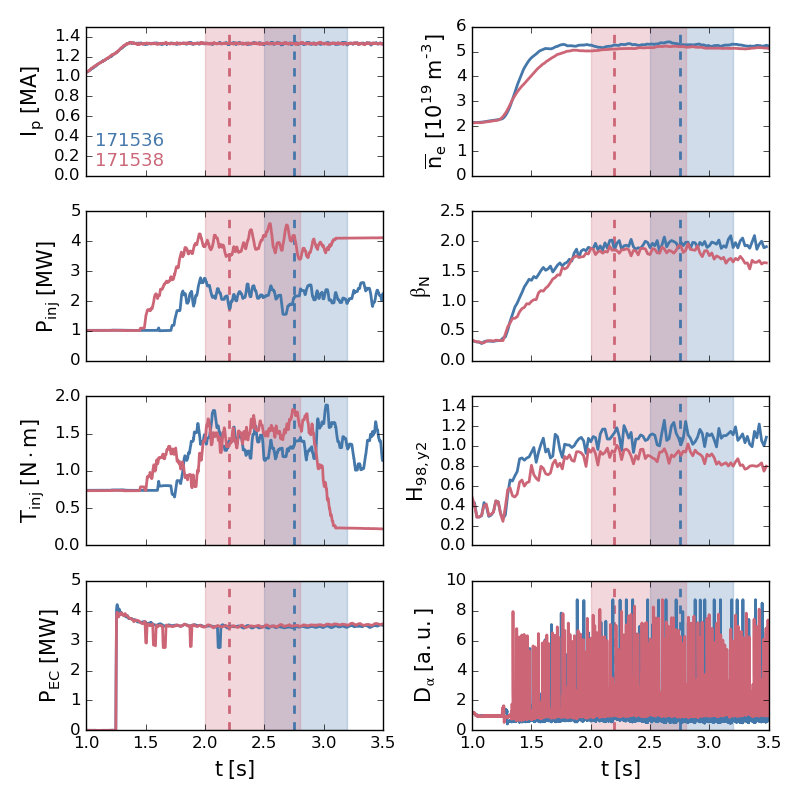
\includegraphics[width = \textwidth]{%
    Chapters/TurbulenceMeasurements/figs/traces.png}
  \caption[Time histories of various actuators \& plasma parameters]{%
    Time histories of various actuators and plasma parameters:
    (a) electron cyclotron resonance heating (ECH) power $P_{\text{ECH}}$,
    (b) ECH location $\rhoech$,
    (c) neutral beam injected (NBI) power $P_{\text{inj}}$,
    (d) NBI torque $T_{\text{inj}}$,
    (e) line-averaged density $\bar{n}_e$,
    (f) normalized plasma pressure $\beta_N$,
    (g) confinement quality $H_{98,\text{y}2}$, and
    (h) divertor $D_{\alpha}$ light, indicating
    the presence of large and small edge localized modes (ELMs).
  }
\label{fig:TurbulenceMeasurements:traces}
\end{figure}

\begin{figure}
  \centering
  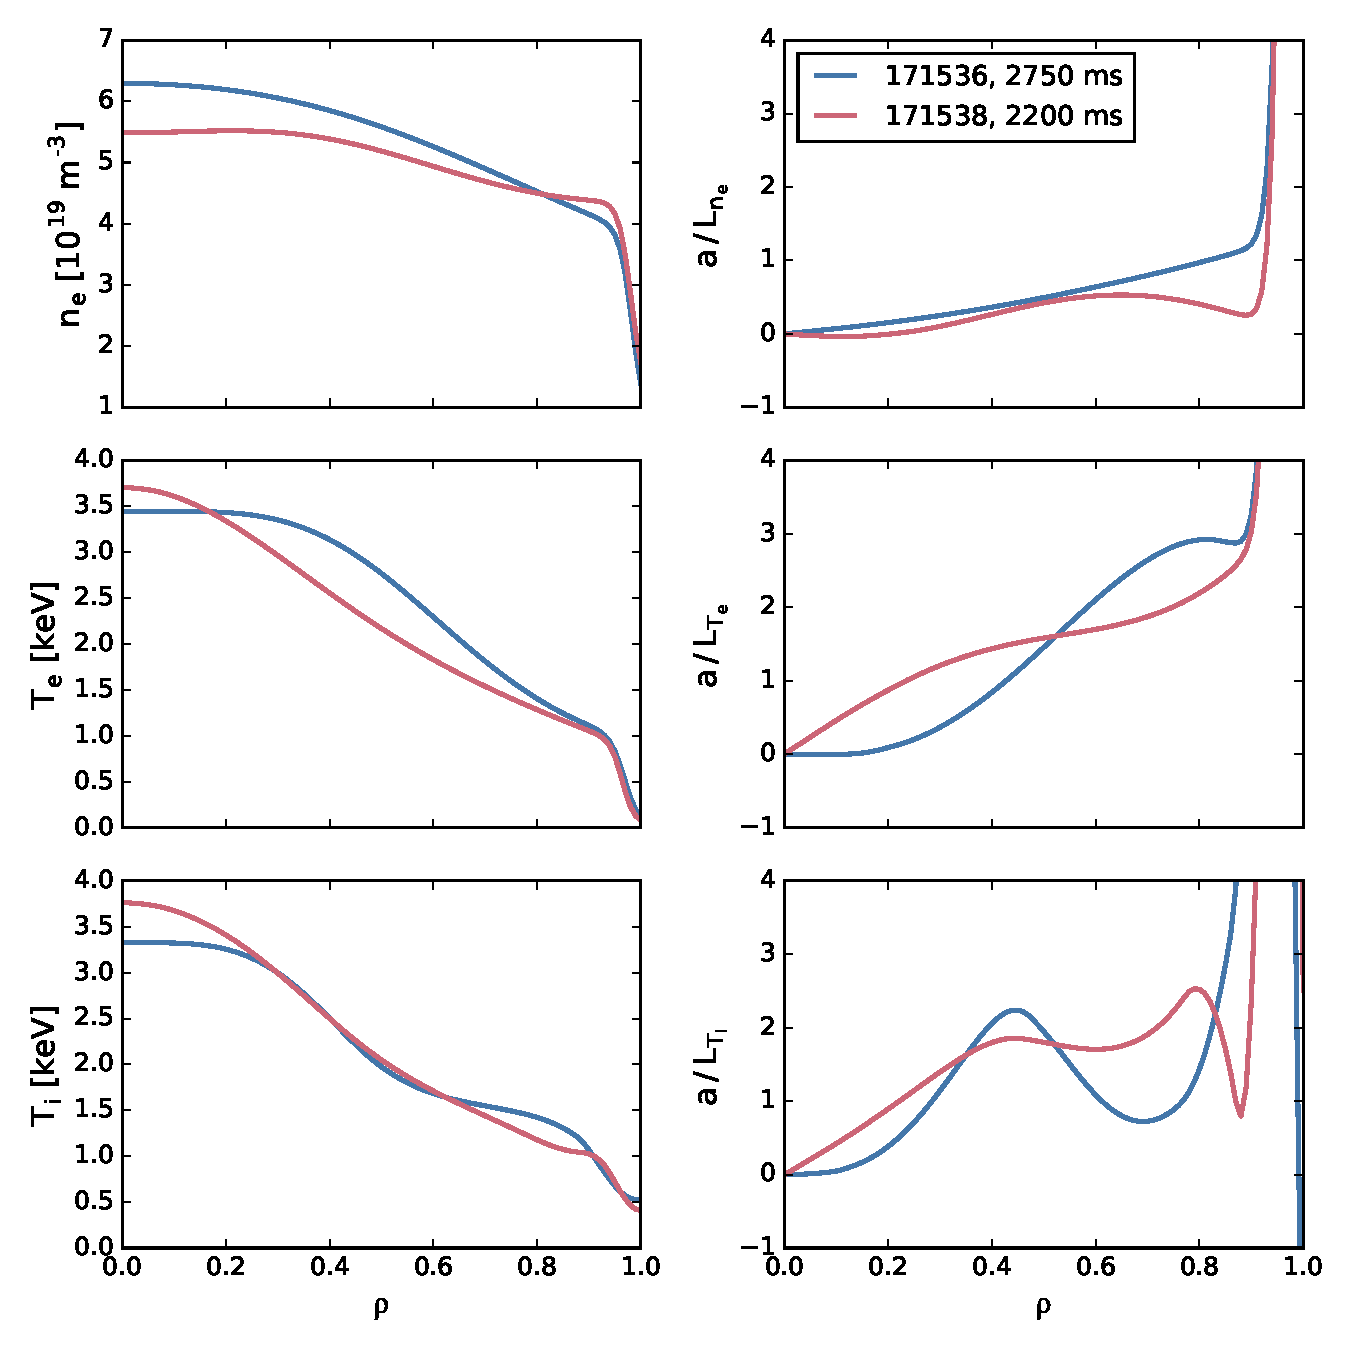
\includegraphics[width = \textwidth]{%
    Chapters/TurbulenceMeasurements/figs/profiles.pdf}
  \caption[Equilibrium profiles, inverse scale lengths, \& $\ExB$ shearing rate]{%
    Profiles, normalized inverse scale lengths, and $\ExB$ shearing rate:
    (a) electron density $n_e$,
    (b) electron temperature $T_e$,
    (c) deuterium temperature $T_i$,
    (d) radial electric field $E_r$ along the outboard midplane,
    (e) normalized inverse $n_e$ scale length $a / L_{n_e}$,
    (f) normalized inverse $T_e$ scale length $a / L_{T_e}$,
    (g) normalized inverse $T_i$ scale length $a / L_{T_i}$,
    (h) $\ExB$ shearing rate $\gamma_E$.
    The shaded bands indicate the $1\sigma$ uncertainties in the profiles,
    as determined by performing separate fits to $100$ distinct data sets
    generated via Monte Carlo variation
    of the measurements about their uncertainties.
    Representative measurements and their uncertainties are indicated
    for a $\SI{10}{\milli\second}$ window from a single shot.
    The relatively large uncertainty on $\gamma_E$
    is dominated by uncertainty in the curvature
    of the $T_i$ profile.
  }
\label{fig:TurbulenceMeasurements:profiles}
\end{figure}

Equilibrium profiles were obtained
by averaging over $\SI{200}{\milli\second}$,
as indicated by the shaded regions
in Figure~\ref{fig:TurbulenceMeasurements:traces}.
Magnetic equilibria were
reconstructed with the EFIT code~\cite{lao_fst05} and
were constrained to match the total plasma pressure and
motional Stark effect (MSE) measurements
of the local magnetic pitch angle.
Electron densities and temperatures
were measured via Thomson scattering, while
ion densities and temperatures
were inferred from charge exchange recombination (CER) measurements
of C$^{6+}$, the dominant impurity in \diiid.
The radial electric field was computed
by invoking force balance on C$^{6+}$.
% (poloidal data for $\rho \geq 0.6)$
To minimize the impact of ELMs on the profile fits,
only measurements falling
within the last {$50\%$ -- $99\%$} of each inter-ELM window
were included in the fitting.
The fitted profiles and
their corresponding gradients or
normalized inverse scale lengths
are shown in
Figure~\ref{fig:TurbulenceMeasurements:profiles}.
While it may seem counterintuitive
that the central electron temperature $T_e(0)$
increases when moving ECH from $\rho = 0.5$ to $\rho = 0.8$,
maintaining constant $\beta_N$
requires increased NBI heating
(see Figure~\ref{fig:TurbulenceMeasurements:traces}(c)),
which enhances the NBI electron heating density $q_{e,\text{NBI}}$
across the full plasma profile,
as shown in Figure~\ref{fig:TurbulenceMeasurements:electron_heating}(b).
The $1\sigma$ uncertainties in the profile fits,
indicated by the shaded bands in
Figure~\ref{fig:TurbulenceMeasurements:profiles},
were quantified by
performing separate fits to $100$ distinct data sets
generated via Monte Carlo variation
of the measurements about their uncertainties.
Clearly, moving ECH from $\rho = 0.5$ to $\rho = 0.8$
produces large changes
in the electron-scale and ion-scale drives,
$a / L_{T_e}$ and $a / L_{T_i}$, respectively,
in the region of the plasma accessible to the PCI probe beam
($R = \SI{1.98}{\meter}$).
Using these profiles,
power-balance analysis was performed
with the ONETWO code~\cite{pfeiffer_onetwo},
with NUBEAM~\cite{pankin_cpc04} calculations
for NBI heating and torque and
TORAY~\cite{matsuda_ieee89} calculations for ECH;
the resulting loop voltages, stored energies, and neutron rates
match their measured values to within $\pm 5\%$.

\begin{figure}
  \centering
  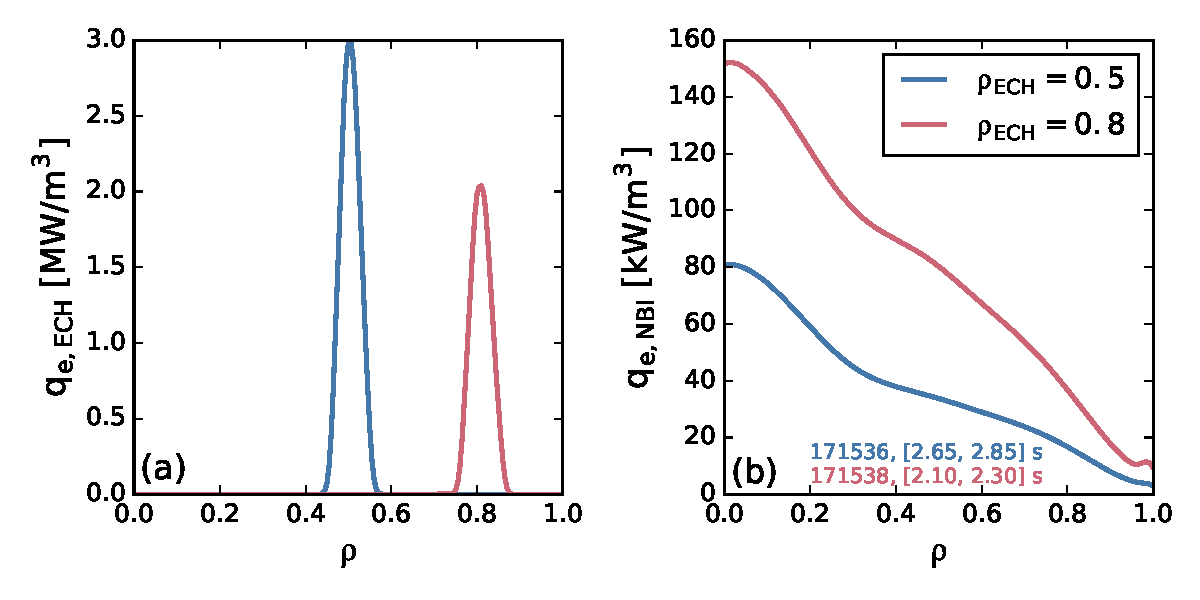
\includegraphics[width = \textwidth]{%
    Chapters/TurbulenceMeasurements/figs/electron_heating.pdf}
  \caption[ECH \& NBI electron-heating profiles]{%
    (a) ECH electron heating density $q_{e,\text{ECH}}$ and
    (b) NBI electron heating density $q_{e,\text{NBI}}$.
    When moving ECH from $\rho = 0.5$ to $\rho = 0.8$,
    maintaining constant $\beta_N$
    requires increased NBI heating
    (see Figure~\ref{fig:TurbulenceMeasurements:traces}(c)),
    which enhances the NBI electron heating density $q_{e,\text{NBI}}$
    across the full plasma profile.
    The radiated power and ohmic heating
    negligibly change between the two discharges.
  }
\label{fig:TurbulenceMeasurements:electron_heating}
\end{figure}


\section{Combined PCI-interferometer measurements}
\label{sec:TurbulenceMeasurements:Measurements}
The experiment described in
Section~\ref{sec:TurbulenceMeasurements:ExperimentalConditions}
presents an ideal opportunity
for multiscale turbulence investigations
with the combined PCI-interferometer.
Below, Section~\ref{sec:TurbulenceMeasurements:Measurements:ELM_filtering}
discusses the automated filtering of transient bursts
attributable to edge localized modes (ELMs)
that would otherwise bias spectral estimates
of the background turbulence.
Section~\ref{sec:TurbulenceMeasurements:Measurements:Sf} then
compares the interferometer and PCI frequency spectra
for $\rhoech = 0.5$ and $\rhoech = 0.8$;
interestingly, the interferometer identifies
a novel turbulent branch with properties
consistent with a micro-tearing mode (MTM).
Next, Section~\ref{sec:TurbulenceMeasurements:Measurements:Skf}
presents the PCI frequency-wavenumber spectra,
which reveal the presence of several distinct turbulent branches.
Finally, Section~\ref{sec:TurbulenceMeasurements:Measurements:Sk}
demonstrates that the PCI wavenumber spectrum
distinctly flattens with $\rhoech = 0.5$
relative to that with $\rhoech = 0.8$,
which is reminiscent of results
from realistic multiscale gyrokinetic simulations.


\subsection{ELM filtering}
\label{sec:TurbulenceMeasurements:Measurements:ELM_filtering}
Edge localized modes (ELMs) expel impurities from the plasma but
will also present severe challenges to plasma-facing components
in future reactors~\cite[Sec.~7.17]{wesson}.
Because of their virulence and their bursty nature,
ELMs produce strong spiking in the interferometer and PCI measurements,
whitening the measured spectra
[Sec.~10.3.2.3]\cite{bendat_and_piersol}.
Additionally, the temperature and density profiles relax during an ELM,
altering the turbulent drives in the plasma edge.
In order to accurately estimate
the spectrum of the background turbulence, then,
the ELM contributions to the interferometer and PCI measurements
must be removed.

\begin{figure}
  \centering
  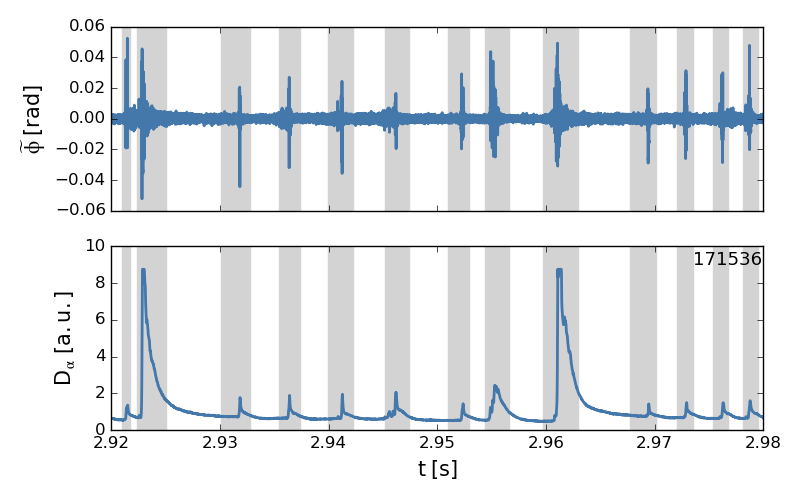
\includegraphics[width = \textwidth]{%
    Chapters/TurbulenceMeasurements/figs/ELM_filtering_example.png}
  \caption[ELM filtering]{%
    Edge localized modes (ELMs) must be removed
    from the PCI and interferometer measurements
    prior to spectral analysis of the background turbulence.
    (Upper panel): The interferometer-measured
    fluctuating phase $\tilde{\phi}$,
    with large, ELM-induced spiking.
    (Lower panel): Divertor $D_{\alpha}$ emission,
    indicating the presence of large Type I ELMs
    as well as smaller ELMs.
    Windows \emph{excluded} from spectral analysis are shown in gray.
    The \diiid\space shot number is shown in the upper right
    of the lower panel.
  }
\label{fig:TurbulenceMeasurements:ELM_filtering_example}
\end{figure}

In this work, ELMs are simply and automatically detected
using measurements from the interferometer.
After the high-pass filtering described in
Section~\ref{sec:Implementation:DataPreparation:high_pass_filtering},
the interferometer-measured fluctuating phase $\tilde{\phi}$
is a zero-mean, random process,
as shown in the upper panel of
Figure~\ref{fig:TurbulenceMeasurements:ELM_filtering_example}.
Large, intermittent spikes pepper $\tilde{\phi}(t)$ during ELMy H-mode, and
the lower panel of
Figure~\ref{fig:TurbulenceMeasurements:ELM_filtering_example}
indicates that these spikes are well correlated
with ELM-induced $D_{\alpha}$ emission in the divertor.
While the $D_{\alpha}$ emission following large Type I ELMs
exhibits a relatively slow decay,
the interferometer-measured $\tilde{\phi}$
returns to stationarity much more rapidly.
Thus, it is desirable to identify
stationary inter-ELM windows
from the interferometer measurements
rather than the $D_{\alpha}$ emission.
Points in the interferometer-measured $\tilde{\phi}$
exceeding $3 \times$ the RMS value
are identified as ELMs, and
successive ELMs are required to be separated
by at least a $\SI{0.5}{\milli\second}$ ``debouncing time''
(spikes separated by less than the debouncing time
are classified as belonging to the same ELM).
Subsequent spectral analysis is then performed
using only the $20\%$ -- $80\%$ inter-ELM windows
of the interferometer and PCI measurements.
Figure~\ref{fig:TurbulenceMeasurements:ELM_filtering_example}
shows the windows \emph{excluded} from spectral analysis in gray.


\subsection{Frequency spectra}
\label{sec:TurbulenceMeasurements:Measurements:Sf}
One-sided autospectral densities estimates $G_{\phi,\phi}(f)$
of the phase fluctuations
are calculated using the methodology
described in Section~\ref{app:SpectralEstimation:NonParametric}.
The interferometer and PCI signals
from the shaded windows in
Figure~\ref{fig:TurbulenceMeasurements:traces}
are split into realizations of $1024$ points
(corresponding to roughly $\SI{250}{\micro\second}$)
resulting in a frequency resolution
of approximately $\SI{4}{\kilo\hertz}$ in the spectral estimates.
As described in
Section~\ref{sec:TurbulenceMeasurements:Measurements:ELM_filtering},
only realizations falling within
$20\%$ -- $80\%$ of each inter-ELM window
are included in the ensemble averaging;
the exact number of realizations $N_r$
included in each ensemble
depends on the details of the ELM dynamics, but
$N_r \sim 450$ for the shots considered here,
corresponding to a relative random error
in $G_{\phi,\phi}(f)$ of approximately $5\%$.
A Hanning window is applied to each realization
prior to computation of its fast Fourier transform (FFT).
To simplify inter-ELM bookkeeping,
adjacent realizations have zero overlap.
As described in
Section~\ref{sec:Implementation:DataPreparation:high_pass_filtering},
the interferometer and PCI phase signals
are high-pass filtered prior to spectral analysis, and
no further detrending is performed.
The resulting spectral estimates
for $\rhoech = 0.5$ and $\rhoech = 0.8$
are shown in
Figure~\ref{fig:TurbulenceMeasurements:Sf_interferometer_pci}.
The corresponding noise floors are estimated
from $\SI{50}{\milli\second}$ of data
prior to plasma breakdown;
the knee in the PCI noise floor
at approximately $\SI{500}{\kilo\hertz}$
corresponds to the roll-off in the temporal bandwidth
of the PCI detector and its preamplifiers.
As expected theoretically
(see Figure~\ref{fig:InterferometricMethods:interferometric_method_transfer_functions})
and observed empirically in sound-wave calibrations
(see Figure~\ref{fig:Implementation:cross_calibration}),
the PCI is more sensitive than the heterodyne interferometer.

\begin{figure}
  \centering
  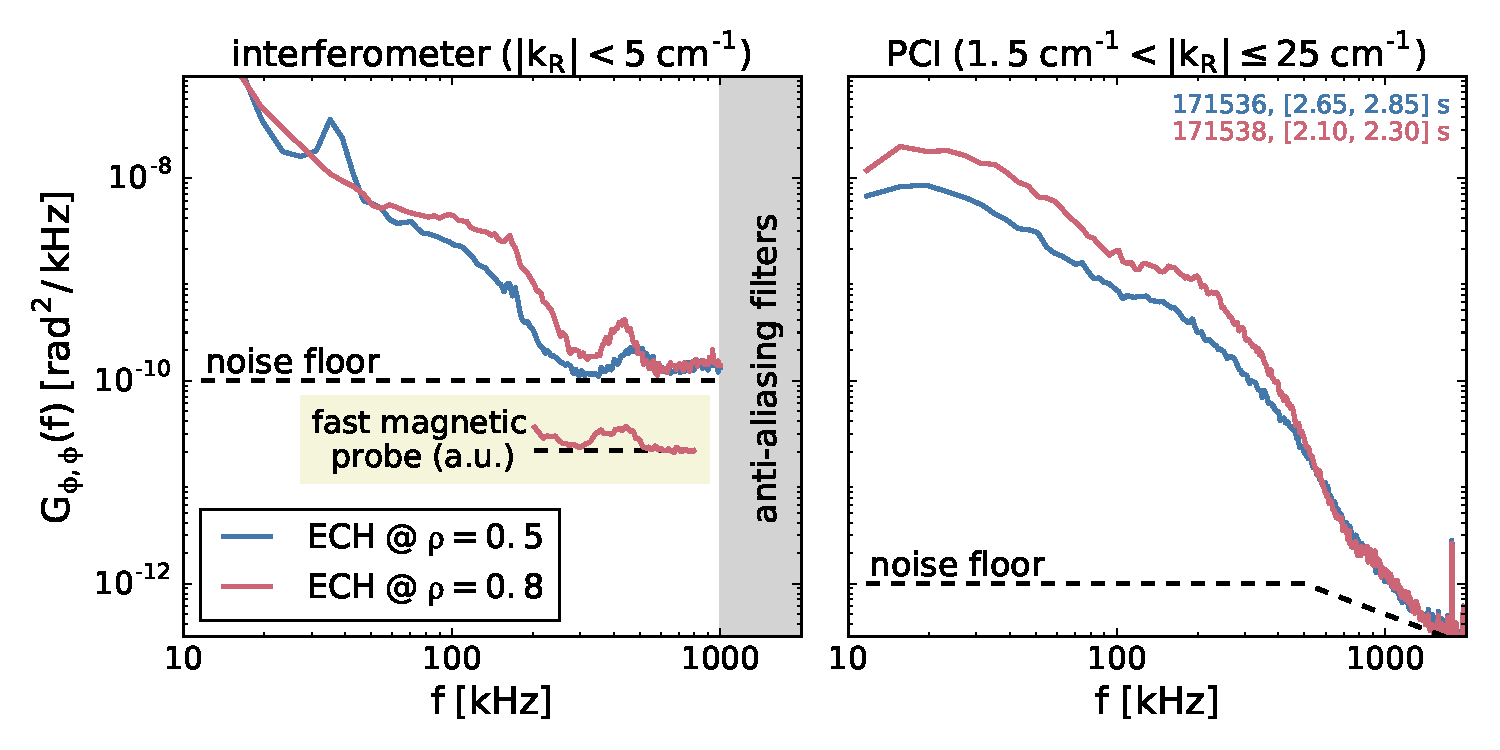
\includegraphics[width = \textwidth]{%
    Chapters/TurbulenceMeasurements/figs/Sf_interferometer_pci.pdf}
  \caption[Interferometer \& PCI frequency spectra]{%
    One-sided autospectral-density estimates $G_{\phi,\phi}(f)$ from
    (a) the heterodyne interferometer and (b) the PCI.
    The low-frequency ($f \lesssim \SI{300}{\kilo\hertz}$) dynamics
    are comparable, with both the interferometer and the PCI
    measuring a $2 - 4\times$ increase in fluctuation power
    when moving from $\rhoech = 0.5$ to $\rhoech = 0.8$.
    The higher-frequency ($f \gtrsim \SI{300}{\kilo\hertz}$) dynamics,
    however, are distinct.
    In particular, the interferometer-measured broadband fluctuation
    between $\SI{300}{\kilo\hertz}$ and $\SI{600}{\kilo\hertz}$
    is low-$k$ (due to its absence in the PCI spectrum),
    electromagnetic (as seen by the beige inset to (a)), and
    driven by collisionality
    (as shown in Figure~\ref{fig:TurbulenceMeasurements:collisionality}),
    suggesting that it may be a micro-tearing mode (MTM).
    The subtle break in slope at $f \sim \SI{800}{\kilo\hertz}$
    in the PCI spectrum when $\rhoech = 0.8$
    is shown to be a distinct turbulent branch
    in Figure~\ref{fig:TurbulenceMeasurements:Skf_pci}.
  }
\label{fig:TurbulenceMeasurements:Sf_interferometer_pci}
\end{figure}

Interestingly, the autospectral density of the heterodyne interferometer
indicates the presence of a distinct broadband fluctuation
with a central frequency $f_0 \sim \SI{450}{\kilo\hertz}$ and
a bandwidth $\Delta f \sim \SI{300}{\kilo\hertz}$.
The toroidally separated $V2$ interferometer
corroborates the presence of this fluctuation, but
the fluctuation is only vaguely coherent between the two interferometers,
with magnitude-squared coherences $\gamma_{xy}^2(f) \leq 0.1$.
The fluctuation is larger than
the corresponding PCI-measured fluctuations
in this frequency range, but
it is absent from the autospectral density of the PCI;
this indicates that the fluctuation wavenumber
is smaller than the PCI low-$k$ cutoff
(\ref{eq:Implementation:kg_realized}).
Further, this fluctuation has a magnetic component,
as shown by the beige inset to
Figure~\ref{fig:TurbulenceMeasurements:Sf_interferometer_pci}(a).
The red curve in the beige inset
corresponds to the autospectral density (in arbitrary units)
of the poloidal magnetic-field fluctuations
measured by a high-frequency magnetic probe ($b5$)~\cite{strait_rsi06}
during the $\rhoech = 0.8$ window, while
the dashed line corresponds to the noise floor,
as estimated from $\SI{50}{\milli\second}$
of data prior to plasma breakdown.
The magnetic autospectral density is estimated
in a manner consistent with those of the interferometer and PCI
(realization length of approximately $\SI{250}{\micro\second}$
with zero overlap between adjacent realizations,
application of Hanning window to each realization prior to FFT computation,
ensemble averaging only over realizations falling within
$20\%$ -- $80\%$ of each inter-ELM window, and
a total number of realizations $N_r \sim 450$).
The autospectral density of the interferometer also
indicates that the power in this fluctuation
increases when moving from
$\rhoech = 0.5$ to $\rhoech = 0.8$.
To prove that this is a robust trend,
the total power in this fluctuation
is computed for stationary windows
from $7$ distinct shots with $\rhoech = 0.5$ and
from $7$ distinct shots with $\rhoech = 0.8$,
each of which are nominally identical
to the corresponding discharges shown in
Figures~\ref{fig:TurbulenceMeasurements:traces} and
\ref{fig:TurbulenceMeasurements:profiles}.
The total fluctuation power is quantified as
\begin{equation}
  \text{var}(\tilde{\phi})
  =
  \int_{\SI{300}{\kilo\hertz}}^{\SI{600}{\kilo\hertz}}
  \left[%
    G_{\phi,\phi}^{\text{int}}(f) - N.F.
  \right] df,
  \label{eq:TurbulenceMeasurements:MTM_power}
\end{equation}
where $G_{\phi,\phi}^{\text{int}}(f)$
is the autospectral density of the heterodyne interferometer and
$N.F. = \SI{e-10}{\radian\squared\per\kilo\hertz}$
is the corresponding noise floor.
\begin{figure}
  \centering
  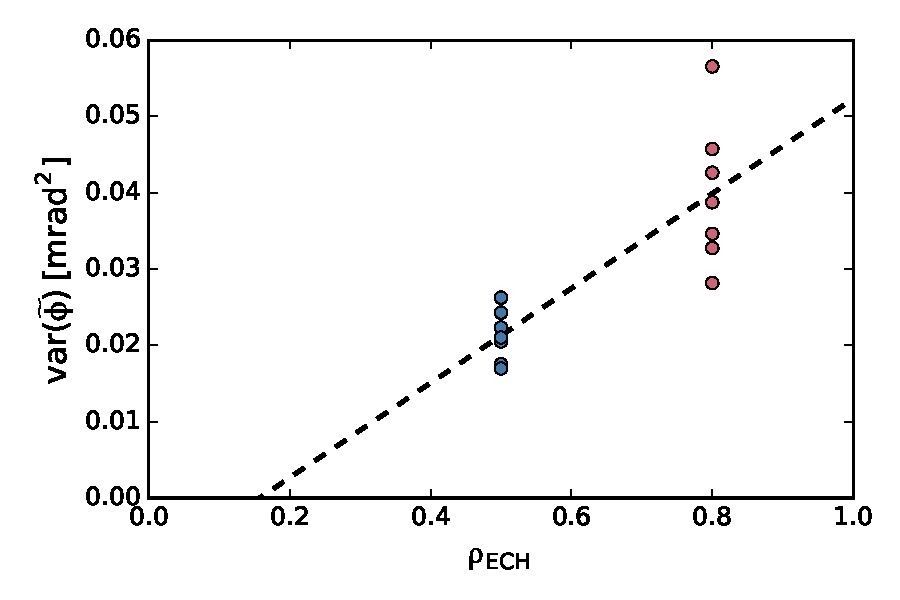
\includegraphics[width = 0.75 \textwidth]{%
    Chapters/TurbulenceMeasurements/figs/interferometer_bump_integrated_power.pdf}
  \caption[Power in low-$k$, mid-$f$, electromagnetic turbulence vs. ECH location]{%
    Power $\text{var}(\tilde{\phi})$ in interferometer-measured
    low-$k$, mid-$f$, electromagnetic turbulence vs. ECH location $\rhoech$.
    Powers are estimated via
    (\ref{eq:TurbulenceMeasurements:MTM_power}).
    Different points correspond to distinct, nominally identical shots
    from the same experimental run day;
    the dashed line is the linear least-squares fit to the points,
    indicating an approximate doubling in fluctuation power
    when moving from $\rhoech = 0.5$ to $\rhoech = 0.8$.
  }
\label{fig:TurbulenceMeasurements:interferometer_bump_integrated_power}
\end{figure}
Figure~\ref{fig:TurbulenceMeasurements:interferometer_bump_integrated_power}
plots $\text{var}(\tilde{\phi})$ versus $\rhoech$;
a linear least-squares fit
indicates that the fluctuation power
approximately doubles when moving
from $\rhoech = 0.5$ to $\rhoech = 0.8$.
Further, Figure~\ref{fig:TurbulenceMeasurements:collisionality}
shows that the electron-ion collisionality $\nu_{ei}$
in the region of the plasma accessible to the PCI probe beam
($R = \SI{1.98}{\meter}$)
also roughly doubles when moving
from $\rhoech = 0.5$ to $\rhoech = 0.8$.
Thus, this fluctuation is
low-$k$, electromagnetic, and driven by collisionality,
suggesting that this fluctuation
may be a micro-tearing mode (MTM)~\cite[Sec.~8.5]{wesson}\cite{drake_pf77},
which is predicted to be marginally unstable
in this experiment's reference discharge~\cite{holland_nf17}.

\begin{figure}
  \centering
  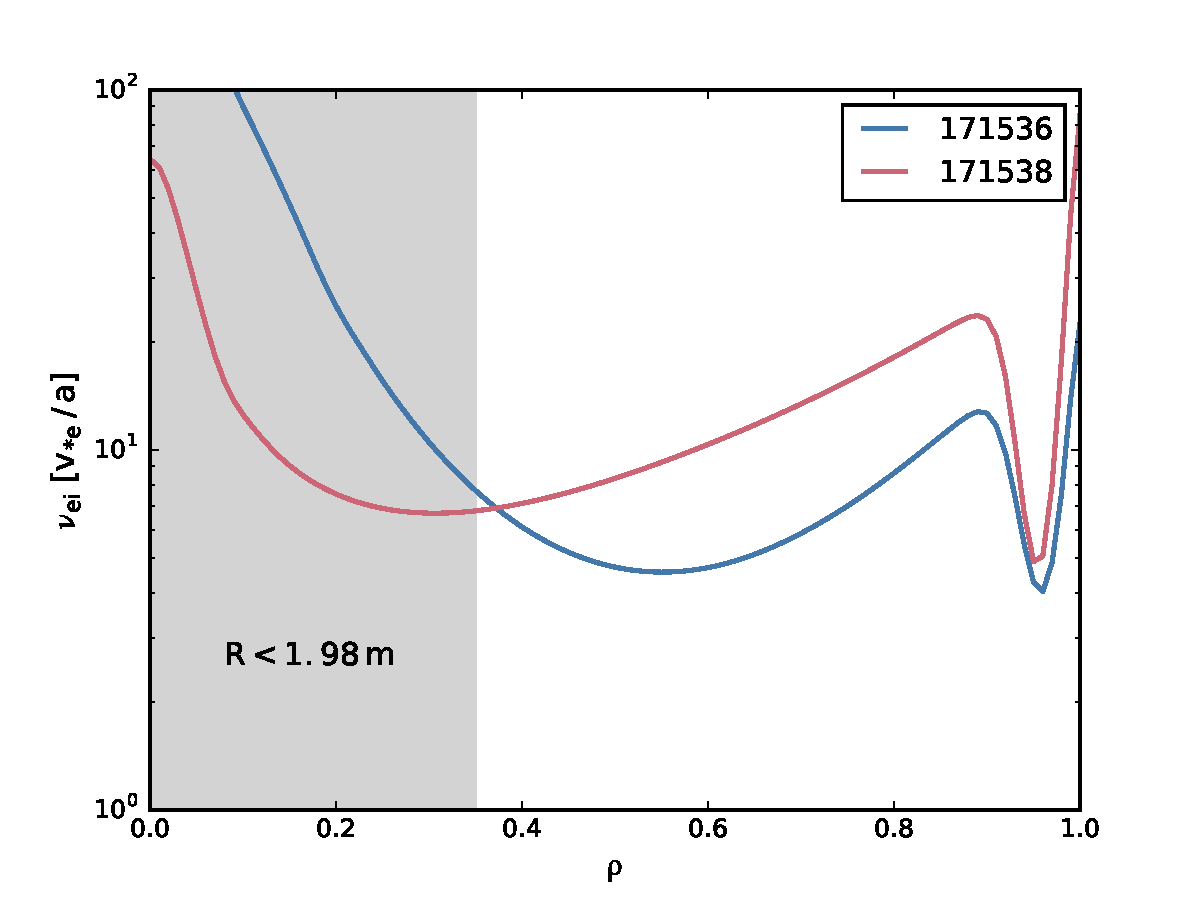
\includegraphics[width = 0.9 \textwidth]{%
    Chapters/TurbulenceMeasurements/figs/collisionality.pdf}
  \caption[Collisionality variation with ECH location]{%
    The electron-ion collisionality $\nu_{ei}$
    in the region of the plasma
    accessible to the PCI probe beam
    ($R = \SI{1.98}{\meter}$)
    roughly doubles when moving
    from $\rhoech = 0.5$ to $\rhoech = 0.8$.
    The collisionality is computed from the profiles in
    Figure~\ref{fig:TurbulenceMeasurements:profiles}, and
    the shaded bands indicate the $1\sigma$ uncertainties.
    The collisionality normalization is $\vmag_{*e} / a$, where
    $\vmag_{*e}$ is the electron diamagnetic velocity and
    $a$ is the minor radius of the plasma;
    note that the angular electron diamagnetic frequency
    $\omega_{*e} \propto \vmag_{*e} / a$~\cite[Sec.~8.2]{wesson} and
    that micro-tearing mode (MTM) linear-stability calculations
    are performed in expansions of $\nu_{ei} / \omega_{*e}$
    \cite[Sec.~8.5]{wesson}\cite{drake_pf77}.
    Unfortunately, without a wavenumber measurement,
    the more theoretically relevant $\omega_{*e}$ normalization
    cannot be performed.
    Both discharges are in the banana regime
    ($\nu_{ei}^* < 1$)~\cite[Sec.~4.6]{wesson}
    for $\rho \lesssim 0.95$.
  }
\label{fig:TurbulenceMeasurements:collisionality}
\end{figure}

It is also interesting to examine
the low-frequency ($f \lesssim \SI{300}{\kilo\hertz}$) fluctuations
measured by both the interferometer and the PCI.
Both systems measure a $2 - 4\times$ increase
in the low-frequency fluctuation power
when moving from $\rhoech = 0.5$ to $\rhoech = 0.8$,
which may be responsible for the slightly reduced confinement
in Figure~\ref{fig:TurbulenceMeasurements:traces}(g).
The spatial content of these fluctuations
can be roughly characterized
via the magnitude-squared coherence $\gamma^2_{xy}(f)$
between the interferometer ($x$) and PCI ($y$) measurements.
As discussed in Section~\ref{app:SpectralEstimation:NonParametric},
$\gamma^2_{xy}(f)$ is bounded between $0$ and $1$, and
it quantifies the linear correlation between signals $x$ and $y$,
with $\gamma^2_{xy}(f) = 0$ indicating $0\%$ correlation at frequency $f$ and
$\gamma^2_{xy}(f) = 1$ indicating $100\%$ correlation at frequency $f$.
Thus, $\gamma^2_{xy}(f)$ characterizes the fraction of fluctuation power
sitting in the mid-$k$ overlap of the interferometer and PCI
\cite[Sec.~5.2.6]{bendat_and_piersol}.
As with the auto-spectral density estimates,
the interferometer and PCI signals
are split into realizations of $1024$ points
with zero overlap between adjacent realizations,
a Hanning window is applied to each realization
prior to computing its FFT,
the ensemble average is performed only over realizations falling within
$20\%$ -- $80\%$ of each inter-ELM window, and
the total number of realizations is $N_r \sim 450$.
The resulting $\gamma^2_{xy}(f)$ estimates
are shown in Figure~\ref{fig:TurbulenceMeasurements:gamma2xy}.
As demonstrated in Section~\ref{sec:TurbulenceMeasurements:Measurements:Skf},
the frequency $f$ of a broadband fluctuation
is often related to its wavenumber $k$ via
$f = \vph k / (2 \pi)$,
where $\vph$ is the lab-frame phase velocity of the fluctuation;
that is, the lowest frequencies in a particular fluctuation branch
are associated with the lowest wavenumbers, and
the highest frequencies in a particular fluctuation branch
are associated with the highest wavenumbers.
Thus, the low values of $\gamma^2_{xy}(f)$
for $f \lesssim \SI{100}{\kilo\hertz}$
in Figure~\ref{fig:TurbulenceMeasurements:gamma2xy}
can be interpreted as the interferometer measuring
substantial power in low-$k$ fluctuations
that sit below the PCI's low-$k$ cutoff
(\ref{eq:Implementation:kg_realized}).
Similarly, the low values of $\gamma^2_{xy}(f)$
for $f \gtrsim \SI{300}{\kilo\hertz}$
correspond to the PCI measuring
substantial power in high-$k$ fluctuations
that sit above the interferometer's high-$k$ cutoff
(\ref{eq:Implementation:kfsv_interferometer_design})
or below the interferometer's noise floor.
Between $\SI{100}{\kilo\hertz}$ and $\SI{300}{\kilo\hertz}$,
$0.25 \lesssim \gamma^2_{xy} \lesssim 0.5$,
indicating between $25\%$ and $50\%$
of the total fluctuation power
sits in the mid-$k$ overlap of the interferometer and the PCI.
Further, moving from $\rhoech = 0.5$ to $\rhoech = 0.8$
produces a substantial increase in $\gamma^2_{xy}(f)$
for $\SI{200}{\kilo\hertz} \lesssim f \lesssim \SI{300}{\kilo\hertz}$,
suggesting that the wavenumbers of these fluctuations decrease
when moving from $\rhoech = 0.5$ to $\rhoech = 0.8$;
this is corroborated by the increase in the lab-frame phase velocity
shown in Figure~\ref{fig:TurbulenceMeasurements:Skf_pci}.

\begin{figure}
  \centering
  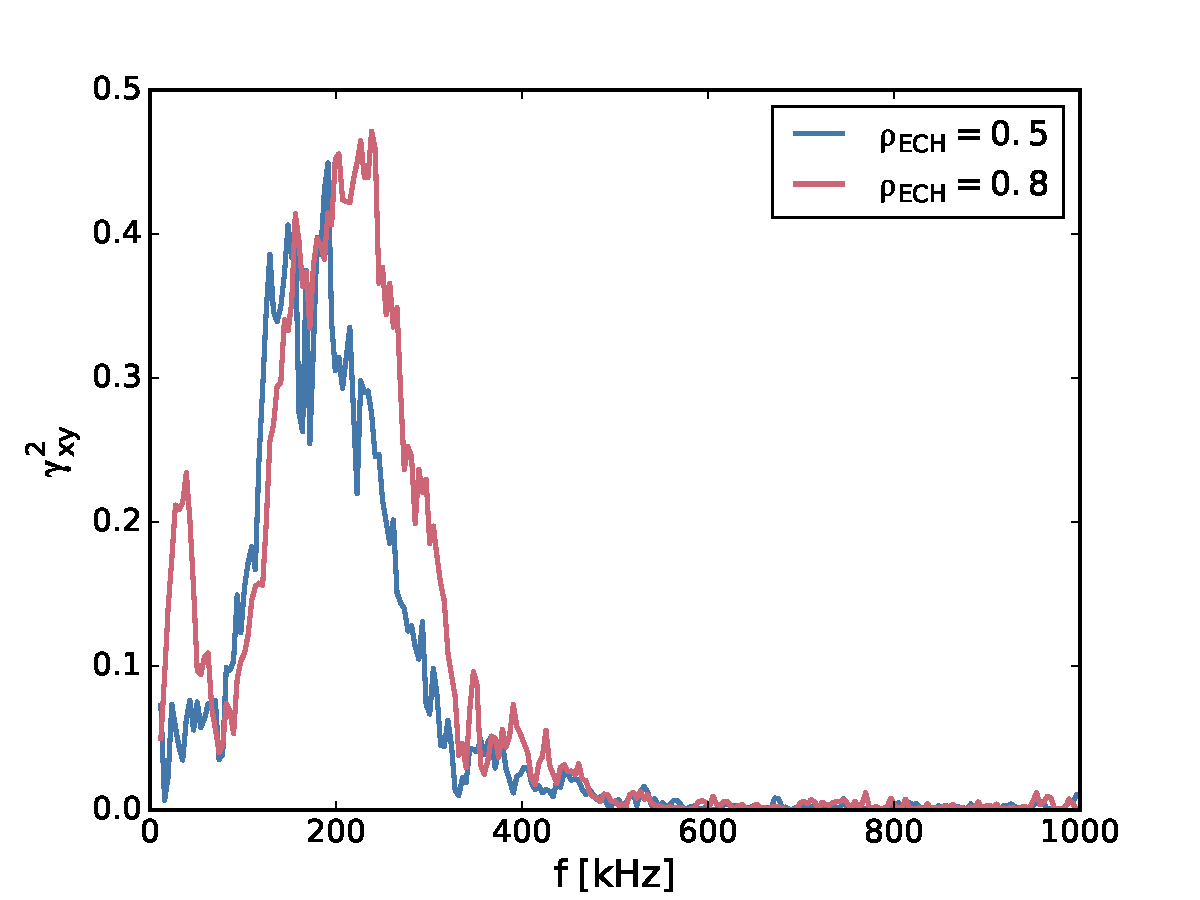
\includegraphics[width = 0.85 \textwidth]{%
    Chapters/TurbulenceMeasurements/figs/coherence.pdf}
  \caption[Magnitude-squared coherence between interferometer \& PCI]{%
    The magnitude-squared coherence $\gamma^2_{xy}(f)$
    between the interferometer and the PCI measurements
    characterizes the fraction of total fluctuation power
    sitting in the mid-$k$ overlap of the interferometer and the PCI.
    The increase in $\gamma^2_{xy}(f)$
    between $\SI{200}{\kilo\hertz}$ and $\SI{300}{\kilo\hertz}$
    when moving from
    $\rhoech = 0.5$ to $\rhoech = 0.8$
    suggests a wavenumber downshift in these fluctuations, which
    is corroborated by the increase in the lab-frame phase velocity
    shown in Figure~\ref{fig:TurbulenceMeasurements:Skf_pci}.
  }
  \label{fig:TurbulenceMeasurements:gamma2xy}
\end{figure}


\subsection{Frequency-wavenumber spectra}
\label{sec:TurbulenceMeasurements:Measurements:Skf}
As the PCI measurements are made
with a multi-element detector array,
the spatial content of the PCI signal
can also be characterized.
The two-dimensional autospectral density $S_{\phi,\phi}(k,f)$
simultaneously quantifies the spatial and temporal content of a signal.
(Unfortunately, as the interferometer measurements
are currently made with a single-element detector,
$S_{\phi,\phi}(k, f)$ cannot be estimated
from the interferometer measurements;
the only spatial knowledge about the interferometer signal
is that the wavenumber magnitudes $|k|$
sit below the interferometer's high-$k$ cutoff
(\ref{eq:Implementation:kfsv_interferometer_design})).

The PCI $S_{\phi,\phi}(k, f)$ is estimated using the hybrid
non-parametric-in-time, parametric-in-space technique
discussed in Section~\ref{app:SpectralEstimation:2d_spectra:2d_spectra}.
Specifically, the hybrid autocorrelation function
$\tilde{R}_{\phi,\phi}(\delta, f)$ is estimated non-parametrically
over the shaded windows in Figure~\ref{fig:TurbulenceMeasurements:traces}
via (\ref{eq:SpectralEstimation:hybrid_autocorrelation_estimate})
using the same spectral-estimation parameters as those
in Section~\ref{sec:TurbulenceMeasurements:Measurements:Sf}
(i.e.\ realization length of $1024$ points with
zero overlap between adjacent realizations,
application of Hanning window to each realization prior to FFT computation,
ensemble averaging only over realizations falling within
$20\%$ -- $80\%$ of each inter-ELM window, and
a total number of realizations $N_r \sim 450$).
Then, a parametric $p = 6$ Burg autoregression (AR)
in the spatial lag $\delta$
estimates the autospectral density $S_{\tilde{R},\tilde{R}}(k,f)$
of $\tilde{R}(\delta, f)$, and
the autospectral density $S_{\phi,\phi}(k, f)$
of the phase fluctuations is computed
via (\ref{eq:SpectralEstimation:autospectral_density_Burg}).
The Burg AR is evaluated
on a uniformly spaced, $1000$-element wavenumber grid.
Often, an AR model is referred to as an ``all-pole model''
because the only frequency dependence in the spectral estimate
appears in the denominator;
this all-pole feature of an AR model
allows fitting very sharp spectral features and
substantially improves the wavenumber resolution
of the sparsely sampled (in space) PCI data
(see Figure~\ref{fig:SpectralEstimation:Skf_example}
for a comparison to a conventional Fourier-in-space estimate).

\begin{figure}
  \centering
  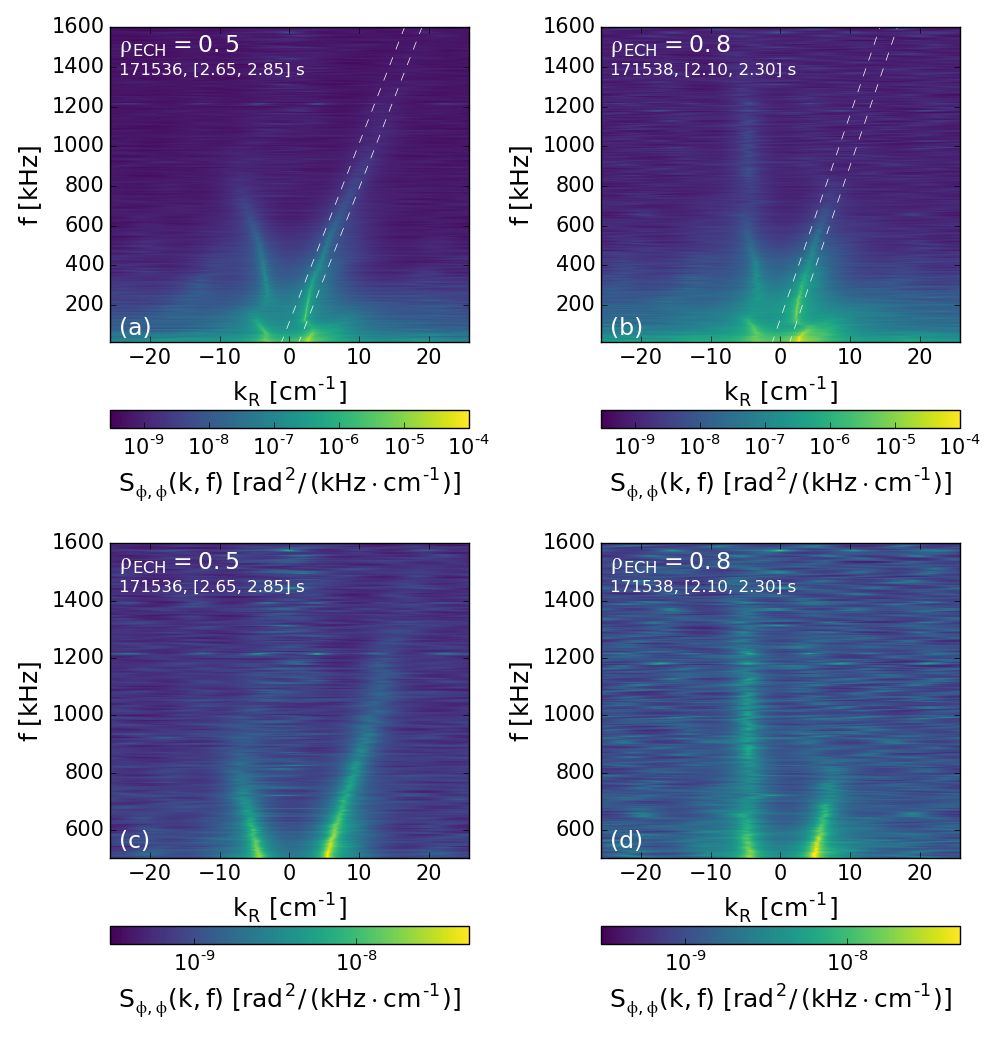
\includegraphics[width = \textwidth]{%
    Chapters/TurbulenceMeasurements/figs/Skf_pci_zoom.png}
  \caption[PCI frequency-wavenumber spectra]{%
    PCI two-dimensional autospectral densities $S_{\phi,\phi}(k, f)$
    for (a) $\rhoech = 0.5$ and (b) $\rhoech = 0.8$.
    To better resolve the high-$k$ and high-$f$ features,
    (c) and (d) display the same spectra from (a) and (b), respectively,
    but only for $f \geq \SI{500}{\kilo\hertz}$ and
    with an altered colorscale.
    Moving from $\rhoech = 0.5$ to $\rhoech = 0.8$
    increases the lab-frame phase velocity but
    decreases the spatiotemporal bandwidth
    of the broadband turbulence bounded by
    the annotating dashed white lines and
    also excites a new turbulent branch
    at $k \sim \SI{-5}{\per\centi\meter}$ and
    $f \sim \SI{1}{\mega\hertz}$.
  }
\label{fig:TurbulenceMeasurements:Skf_pci}
\end{figure}

The PCI $S_{\phi,\phi}(k, f)$
for $\rhoech = 0.5$ and $\rhoech = 0.8$ are shown in
Figure~\ref{fig:TurbulenceMeasurements:Skf_pci}.
The spectra indicate the existence of numerous turbulent branches,
each of which may respond differently when $\rhoech$ is varied.
Two of these branches are discussed here.
First, perhaps one of the most surprising qualitative effects
of moving $\rhoech = 0.5$ to $\rhoech = 0.8$
is the excitation of a new, distinct turbulent mode
at $k_R \sim \SI{-5}{\per\centi\meter}$
with a central frequency $f_0 \sim \SI{1}{\mega\hertz}$ and
a bandwidth $\Delta f \sim \SI{400}{\kilo\hertz}$.
This mode corresponds to the subtle break in slope
at $f \sim \SI{800}{\kilo\hertz}$ in the PCI $G_{\phi,\phi}(f)$
in Figure~\ref{fig:TurbulenceMeasurements:Skf_pci}.
This mode straddles
the current spatiotemporal limits of the interferometer and
sits well below the interferometer noise floor;
thus, this mode is invisible to the interferometer.
The mode is robustly observed in all $7$
of the steady-state $\rhoech = 0.8$ windows
from this experimental run day, and
it is robustly absent from all $7$
of the corresponding $\rhoech = 0.5$ windows.
It should be noted that
the PCI observes a similar mode
during ELM-free H-mode and
wide-pedestal QH-mode~\cite{rost_med_k_high_f_mode}
as well as during NBI-only ELMy H-mode
(see Figure~\ref{fig:SpectralEstimation:Skf_example}).
Second, and perhaps of more relevance to multiscale studies,
is the turbulent branch
bounded by the annotating dashed white lines
in Figure~\ref{fig:TurbulenceMeasurements:Skf_pci}.
When $\rhoech = 0.5$,
this turbulent branch
has a lab-frame phase velocity
$\vph = \SI{5.6}{\kilo\meter\per\second}$
with wavenumbers and frequencies extending to
$\SI{14}{\per\centi\meter}$ and $\SI{1250}{\kilo\hertz}$, respectively;
moving to $\rhoech = 0.8$
increases the lab-frame phase velocity to
$\vph = \SI{6.5}{\kilo\meter\per\second}$
but reduces the spatiotemporal bandwidth to
$\SI{7.2}{\per\centi\meter}$ and $\SI{750}{\kilo\hertz}$.
These observations are generic to all $7$
of the steady-state $\rhoech = 0.5$ windows
and all $7$ of the steady-state $\rhoech = 0.8$ windows
from this experimental run day.
Note that for a given frequency $f$,
an increase in phase velocity
corresponds to a wavenumber downshift
such that the observed change in $\vph$ with $\rhoech$
confirms the wavenumber-downshift speculation
from Figure~\ref{fig:TurbulenceMeasurements:gamma2xy}.
This turbulent branch will be investigated further
in Section~\ref{sec:TurbulenceMeasurements:Measurements:Sk}.


\subsection{Wavenumber spectra}
\label{sec:TurbulenceMeasurements:Measurements:Sk}
Because simulations are finely sampled in space
but often have limited temporal histories,
experimental wavenumber spectra
are particularly valuable for validating
theoretical models and computational predictions.
The PCI wavenumber autospectral density $S_{\phi,\phi}(k)$
corresponding to a given turbulent branch
is computed by integrating the
two-dimensional autospectral density $S_{\phi,\phi}(k, f)$
from Section~\ref{sec:TurbulenceMeasurements:Measurements:Skf}
over the temporal bandwidth $\Delta f$ of the turbulent branch, i.e.\
\begin{equation}
  S_{\phi,\phi}(k)
  =
  \int_{f_0(k) - (\Delta f / 2)}^{f_0(k) + (\Delta f / 2)}
  S_{\phi,\phi}(k, f) df,
\end{equation}
where $f_0(k) = k \vph / (2 \pi)$
is the central frequency of the turbulent branch at wavenumber $k$, and
$\vph$ is the lab-frame phase velocity of the turbulent branch.
Note that restricting the integration domain in this manner
minimizes contributions to $S_{\phi,\phi}(k)$
from noise outside of the branch's bandwidth.
For example, integrating between the bounds
denoted by the annotating dashed white lines
in Figure~\ref{fig:TurbulenceMeasurements:Skf_pci}
produces the $S_{\phi,\phi}(k)$ displayed
in Figure~\ref{fig:TurbulenceMeasurements:Sk_power_law}.
Note that the $\rhoech = 0.5$ spectrum
is substantially flattened (i.e.\ decays more slowly)
relative to the $\rhoech = 0.8$ spectrum.
As shown in Figure~\ref{fig:TurbulenceMeasurements:profiles},
relative to $\rhoech = 0.8$,
$\rhoech = 0.5$ corresponds to
increased $a / L_{Te}$ and decreased $a / L_{T_i}$
over the majority of the plasma
accessible to the PCI probe beam
($R = \SI{1.98}{\meter}$).
This spectral flattening with
enhanced electron-scale drive relative to ion-scale drive
is reminiscent of results from
multiscale gyrokinetic simulations~\cite{howard_pp16}
of an ion cyclotron resonance heated (ICRH)~\cite[Sec.~5.8]{wesson}
L-mode discharge in Alcator C-Mod~\cite[Sec.~11.5]{wesson}.
While the only existing, realistic, multiscale gyrokinetic simulations
of \diiid\space correspond to the reference discharge
for the multiscale experiment discussed here,
the $\ExB$ shearing rate $\gamma_E$ was varied
rather than $a / L_{T_e}$ or $a / L_{T_i}$~\cite{holland_nf17}.
Thus, the spectral flattening observed
in Figure~\ref{fig:TurbulenceMeasurements:Sk_power_law}
with increased $a / L_{T_e}$ and decreased $a / L_{T_i}$
eagerly awaits quantitative comparison
to corresponding multiscale gyrokinetic simulations,
which are expected to be completed by Howard \emph{et al.}
in roughly the next six months.

\begin{figure}
  \centering
  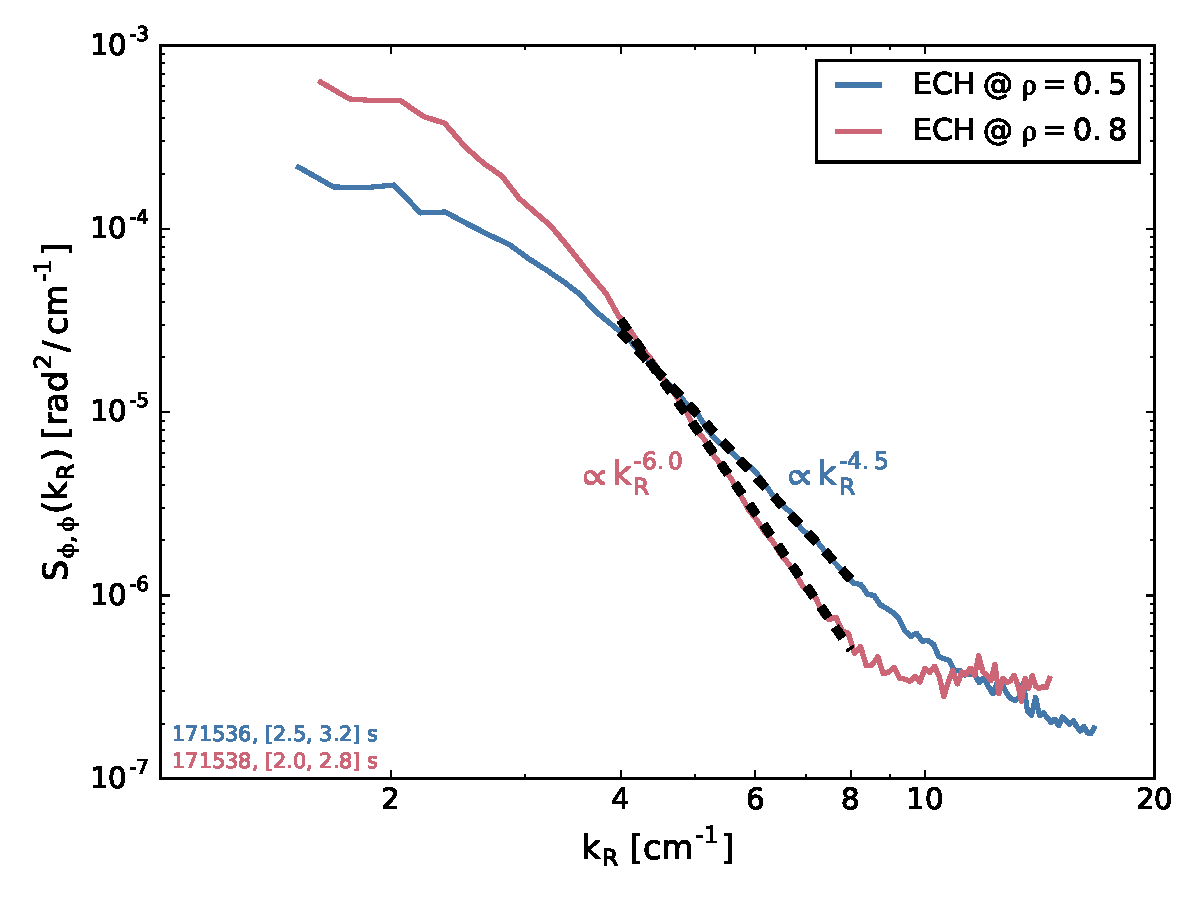
\includegraphics[width = 0.9 \textwidth]{%
    Chapters/TurbulenceMeasurements/figs/Sk_power_law.pdf}
  \caption[PCI frequency-wavenumber spectra]{%
    PCI wavenumber autospectral densities $S_{\phi,\phi}(k)$
    obtained by integrating $S_{\phi,\phi}(k, f)$ in frequency
    between the bounds denoted by the annotating dashed while lines
    in Figure~\ref{fig:TurbulenceMeasurements:Skf_pci}.
    Here, the black dashed lines indicate least-squares power-law fits
    to $S_{\phi,\phi}(k)$.
    The flattening (i.e.\ slower decay) of $S_{\phi,\phi}(k)$
    with $\rhoech = 0.5$ relative to that with $\rhoech = 0.8$
    is reminiscent of results from multiscale gyrokinetic simulations
    in Alcator C-Mod, but
    quantitative comparisons await
    completion of the corresponding multiscale gyrokinetic simulations
    in \diiid.
  }
\label{fig:TurbulenceMeasurements:Sk_power_law}
\end{figure}


\section{TGLF modeling}
\label{sec:TurbulenceMeasurements:Modeling}
To aid the interpretation of the combined PCI-interferometer measurements
described in Section~\ref{sec:TurbulenceMeasurements:Measurements},
linear-stability analysis and quasilinear-transport modeling
were performed with the TGLF code~\footnote{%
  TGLF simulations were graciously performed by Dr. Alessandro Marinoni, but
  the subsequent analysis is the author's own.
}.
Below, Section~\ref{sec:TurbulenceMeasurements:Modeling:TGLF_overview}
provides a brief overview of the TGLF code, and
Section~\ref{sec:TurbulenceMeasurements:Modeling:linear_stability_overview}
presents a global overview
of the TGLF-predicted linear stability
for $\rhoech = 0.5$ to $\rhoech = 0.8$.
In order to facilitate comparisons
between theory and measurement,
Section~\ref{sec:TurbulenceMeasurements:Modeling:wavevectors}
then derives the relationship between
the theoretically relevant field-aligned wavenumber $k_y$ and
the PCI-measured major-radial wavenumber $k_R$.
Next, in an attempt to localize analysis of the TGLF results,
Section~\ref{sec:TurbulenceMeasurements:Modeling:phase_velocity_comparison}
compares the advection of the TGLF-predicted instabilities
by the $\ExB$ velocity
to the PCI-measured phase velocities;
the comparison suggests that
the PCI-measured branch of interest is localized to
$0.6 \leq \rho \leq 0.65$.
Finally, Section~\ref{sec:TurbulenceMeasurements:Modeling:local}
compares the TGLF-predicted electron-density fluctuation spectrum
to the corresponding PCI measurements,
finding qualitative agreement.


\subsection{TGLF overview}
\label{sec:TurbulenceMeasurements:Modeling:TGLF_overview}
TGLF is a gyro-Landau fluid (GLF) model
that captures the dynamics of
both trapped (T) and passing particles
in shaped geometry with finite aspect ratio and $\ExB$ shear
\cite{staebler_pp05, staebler_pp07}.
A GLF model consists of velocity-moment equations
of the gyroaveraged kinetic equation
with moment closures selected
to retain important kinetic effects,
such as Landau damping.
Due to their reduced dimensionality,
GLF models are computationally less expensive
than full gyrokinetic simulations.
TGLF can solve for the linear eigenmodes of
trapped ion and electron modes (TIM and TEM, respectively),
ion and electron temperature gradient (ITG and ETG, respectively) modes,
and kinetic ballooning modes (KBM).
Unfortunately, the default eigenfunction basis
of four Hermite polynomials is typically insufficient
to resolve micro-tearing modes (MTMs)~\cite{staebler_MTM_question}, so
there are no attempts to simulate the MTM in this work.
TGLF additionally uses its eigenmodes
to predict quasilinear transport
using a saturation model fit to results
from nonlinear gyrokinetic simulations~\cite{staebler_pp07},
the most recent of which include
realistic multiscale physics~\cite{staebler_nf17}.


\subsection{Global overview of predicted linear stability}
\label{sec:TurbulenceMeasurements:Modeling:linear_stability_overview}
Using the TGLF\_scan module
in the OMFIT integrated modeling framework~\cite{omfit_nf15},
TGLF simulations were run
to investigate the change in linear stability
when moving from $\rhoech = 0.5$ to $\rhoech = 0.8$.
The simulations span
$0.1 \leq k_y \rho_s \leq 24$ and
$0.3 \leq \rho \leq 0.9$
(only $\rho \gtrsim 0.35$
is accessible to the PCI probe beam, which
propagates vertically through the plasma
at major radius $R = \SI{1.98}{\meter}$).
The equilibrium profiles shown
in Figure~\ref{fig:TurbulenceMeasurements:profiles}
were used as input to TGLF.
Figure~\ref{fig:TurbulenceMeasurements:linear_stability_overview}
displays the resulting linear growth rates $\gamma$ and
plasma-frame phase velocities $\vph = \omega / k_y$
as a function of radial position $\rho$ and
normalized fluctuation wavenumber $k_y \rho_s$.
The predicted change in linear stability
when moving from $\rhoech = 0.5$ to $\rhoech = 0.8$
is largely in accord with intuition
derived from the changes to the normalized inverse scale lengths
shown in Figure~\ref{fig:TurbulenceMeasurements:profiles}(e)-(g).
Perhaps the most substantial change
is that $\rhoech = 0.5$ destabilizes a continuum of
mid-$k$ ($0.5 \lesssim k_y \rho_s \lesssim 5$) electron modes
in the outer region ($\rho \gtrsim 0.6$) of the plasma.
Additionally, in the outer region of the plasma ($\rho \gtrsim 0.6$),
the low-$k$ ion modes ($k_y \rho_s \lesssim 0.3$)
are marginally suppressed and
the high-$k$ electron modes ($k_y \rho_s \gtrsim 10$)
are marginally enhanced
relative to $\rhoech = 0.8$.

\begin{figure}
  \centering
  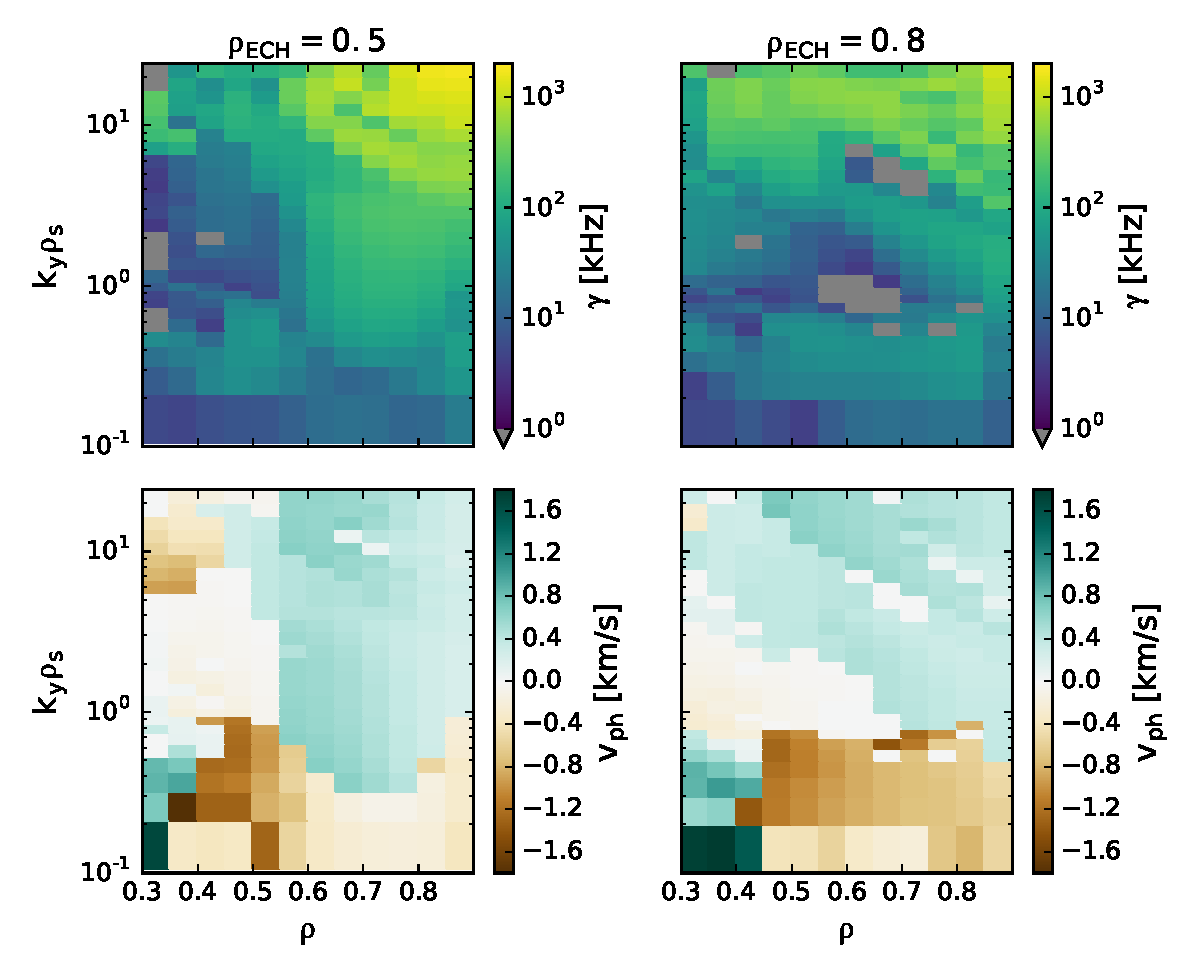
\includegraphics[width = \textwidth]{%
    Chapters/TurbulenceMeasurements/figs/linear_stability_overview.pdf}
  \caption[Global overview of TGLF-predicted linear stability]{%
    Global overview of TGLF-predicted linear stability
    for the profiles shown in
    Figure~\ref{fig:TurbulenceMeasurements:profiles}.
    Linear growth rates $\gamma$ and
    plasma-frame phase velocities $\vph = \omega / k_y$
    are plotted as a function
    of radial position $\rho$ and
    normalized fluctuation wavenumber $k_y \rho_s$
    for $\rhoech = 0.5$ and $\rhoech = 0.8$.
    Electron modes have $\vph > 0$, and
    ion modes have $\vph < 0$.
    The predicted change in linear stability
    when moving from $\rhoech = 0.5$ to $\rhoech = 0.8$
    is largely in accord with intuition
    derived from the changes to the normalized inverse scale lengths
    shown in Figure~\ref{fig:TurbulenceMeasurements:profiles}(e)-(g).
    Growth rates can be compared to
    the $\ExB$ shearing rates $\gamma_E$
    in Figure~\ref{fig:TurbulenceMeasurements:profiles}(h).
  }
\label{fig:TurbulenceMeasurements:linear_stability_overview}
\end{figure}


\subsection{Relation between field-aligned \& PCI-measured wavevectors}
\label{sec:TurbulenceMeasurements:Modeling:wavevectors}
As transport parallel to the magnetic field $\vect{B}$
is much more rapid than transport across the magnetic field,
drift-wave turbulent fluctuations
have a dominant, central wavevector $\vect{k}_0$
that satisfies the field-aligned constraint
$\vect{k}_0 \cdot \vect{B} \approx 0$.
For electrostatic fluctuations,
the magnetic field $\vect{B}$ is well-represented
by the equilibrium field $\Beq$ such that
the field-aligned constraint reduces to
$\vect{k}_0 \cdot \Beq \approx 0$, requiring
\begin{equation}
  \vect{k}_0
  =
  k_{\rho,0} \rhohat
  +
  k_{\theta,0}
  \left[%
    \thetahat
    -
    \left( \frac{B_{\theta,0}}{B_{\zeta,0}} \right) \zetahat
  \right],
  \label{eq:TurbulenceMeasurements:k0}
\end{equation}
where
$k_{\rho,0}$ is the dominant radial wavenumber of the turbulence
(note that velocity shear produces finite $k_{\rho,0}$~\cite{rost_pp14}),
$k_{\theta,0}$ is the dominant poloidal wavenumber of the turbulence,
$B_{\theta,0}$ is the equilibrium poloidal magnetic field,
$B_{\zeta,0}$ is the equilibrium toroidal magnetic field, and
the $(\rho, \theta, \zeta)$ coordinate system
is defined in Figure~\ref{fig:TurbulenceMeasurements:coordinate_geometry}.
Analytic theory and computation are often performed
on field-aligned coordinate systems in which
the $z$-coordinate is along $\Beq$,
the $x$-coordinate is in the radial direction, and
the $y$-coordinate is perpendicular to $\Beq$ but
within a flux surface.
In such a field-aligned coordinate system,
$\vect{k}_0 - k_{\rho,0}\rhohat$
is aligned with the $y$-coordinate
% i.e.\ $\vect{k}_0 = |\vect{k}_0| \hat{\vect{y}}$
such that one is led naturally to define
\begin{equation}
  \vect{k}_y
  =
  k_{\theta,0}
  \left[%
    \thetahat
    -
    \left( \frac{B_{\theta,0}}{B_{\zeta,0}} \right) \zetahat
  \right].
  \label{eq:TurbulenceMeasurements:ky}
\end{equation}
The wavenumber $k_y$ (or its dimensionless equivalent, $k_y \rho_s$)
is an important parameter in the classification and understanding
of turbulent fluctuations.

\begin{figure}
  \centering
  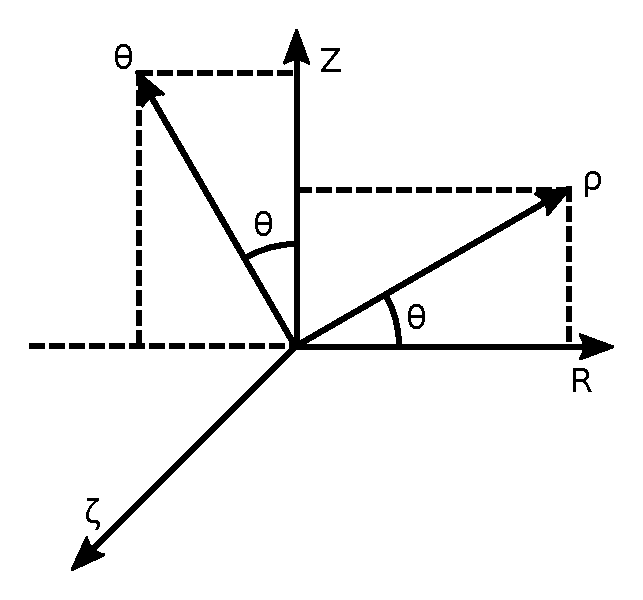
\includegraphics[width = 0.5 \textwidth]{%
    Chapters/TurbulenceMeasurements/figs/coordinate_geometry.pdf}
  \caption[Measurement coordinate system]{%
    Measurement coordinate system.
    Here, $R$ is the major-radial direction,
    $Z$ is the lab-frame vertical direction,
    $\zeta$ is the toroidal angle,
    $\theta$ is the poloidal angle, and
    $\rho$ is a flux-surface label
    corresponding to the square root
    of the normalized toroidal magnetic-field flux.
  }
\label{fig:TurbulenceMeasurements:coordinate_geometry}
\end{figure}

To make contact with theory, then,
it is important to understand the relation between $k_y$ and
the PCI-measured wavevectors.
As a line-integrated measurement,
PCI is sensitive to fluctuations with wavevectors $\kpci$
that are perpendicular to the beam path.
Thus, for the vertical beam path of \diiid's PCI,
\begin{equation}
  \kpci \cdot \Zhat = 0.
  \label{eq:TurbulenceMeasurements:kpci_perp_to_Z}
\end{equation}
As with $\vect{k}_0$, $\kpci$ is also field-aligned
such that (for electrostatic fluctuations)
\begin{equation}
  \kpci \cdot \Beq \approx 0.
  \label{eq:TurbulenceMeasurements:kpci_perp_to_B0}
\end{equation}
In general, $\kpci \neq \vect{k}_0$.
Instead, it is suitable to define
\begin{equation}
  \kpci = \vect{k}_0 + \delta \vect{k}.
  \label{eq:TurbulenceMeasurements:kpci_general}
\end{equation}
The PCI will measure finite signal only if
there exists a $\delta\vect{k}$
within the spatial bandwidth $\Delta\vect{k}$ of the turbulence
such that the resulting $\kpci$ from
(\ref{eq:TurbulenceMeasurements:kpci_general})
satisfies both
(\ref{eq:TurbulenceMeasurements:kpci_perp_to_Z}) and
(\ref{eq:TurbulenceMeasurements:kpci_perp_to_B0}).
(Note that the above reasoning also holds
for any other vertically line-integrated measurement
of field-aligned turbulence,
such as those made by the heterodyne interferometer
constructed in this work).
Decomposing $\delta\vect{k}$
in the $(\rho, \theta, \zeta)$ coordinate system
defined in Figure~\ref{fig:TurbulenceMeasurements:coordinate_geometry}
such that
$\delta\vect{k}
=
\delta k_{\rho} \rhohat
+
\delta k_{\theta} \thetahat
+
\delta k_{\zeta} \zetahat$,
constraint (\ref{eq:TurbulenceMeasurements:kpci_perp_to_Z}) requires
\begin{equation}
  \delta k_{\rho}
  =
  -\delta k_{\rho,0}
  -
  (k_{\theta,0} + \delta k_{\theta}) \cot\theta,
  \label{eq:TurbulenceMeasurements:delta_krho}
\end{equation}
and constraint (\ref{eq:TurbulenceMeasurements:kpci_perp_to_B0}) requires
\begin{equation}
  \delta k_{\zeta}
  =
  -\left( \frac{B_{\theta,0}}{B_{\zeta,0}} \right) \delta k_{\theta}.
  \label{eq:TurbulenceMeasurements:delta_kzeta}
\end{equation}
Using (\ref{eq:TurbulenceMeasurements:delta_krho}) and
(\ref{eq:TurbulenceMeasurements:delta_kzeta}),
$\kpci$ from (\ref{eq:TurbulenceMeasurements:kpci_general}) reduces to
\begin{equation}
  \kpci
  =
  -\left(%
    \frac{k_{\theta,0} + \delta k_{\theta}}{\sin\theta}
  \right)
  \left[%
    \Rhat
    +
    \left( \frac{B_{\theta,0} \sin\theta}{B_{\zeta,0}} \right) \zetahat
  \right],
  \label{eq:TurbulenceMeasurements:kpci_explicit}
\end{equation}
where $\Rhat$ is the unit vector in the major-radial direction and
is related to $\rhohat$ and $\thetahat$
as defined in Figure~\ref{fig:TurbulenceMeasurements:coordinate_geometry}.
Because $|B_{\theta,0}| \ll |B_{\zeta,0}|$,
the PCI is sensitive to fluctuations
with wavevectors that are predominantly in the major-radial direction.
If measurements are made with a one-dimensional detector array,
only a projection of $\kpci$ can be reconstructed.
The one-dimensional detector array of the \diiid\space PCI
is nominally aligned in the major-radial direction
such that the major-radial wavenumber $k_R$ of $\kpci$
can be reconstructed, i.e.\
\begin{equation}
  k_R
  =
  \kpci \cdot \Rhat
  =
  -\left(%
    \frac{k_{\theta,0} + \delta k_{\theta}}{\sin\theta}
  \right)
  \label{eq:TurbulenceMeasurements:kR}.
\end{equation}
In subsequent numerical evaluations,
it is assumed that
$|\delta k_{\theta}| \ll |k_{\theta,0}|$
in order to relate the field-aligned $k_y$ from TGLF
to the PCI-measured major radial wavenumber $k_R$.
Figure~\ref{fig:TurbulenceMeasurements:wavenumber_conversion}
displays profiles of $|k_y \rho_s|$ for various $k_R$ of interest.

\begin{figure}
  \centering
  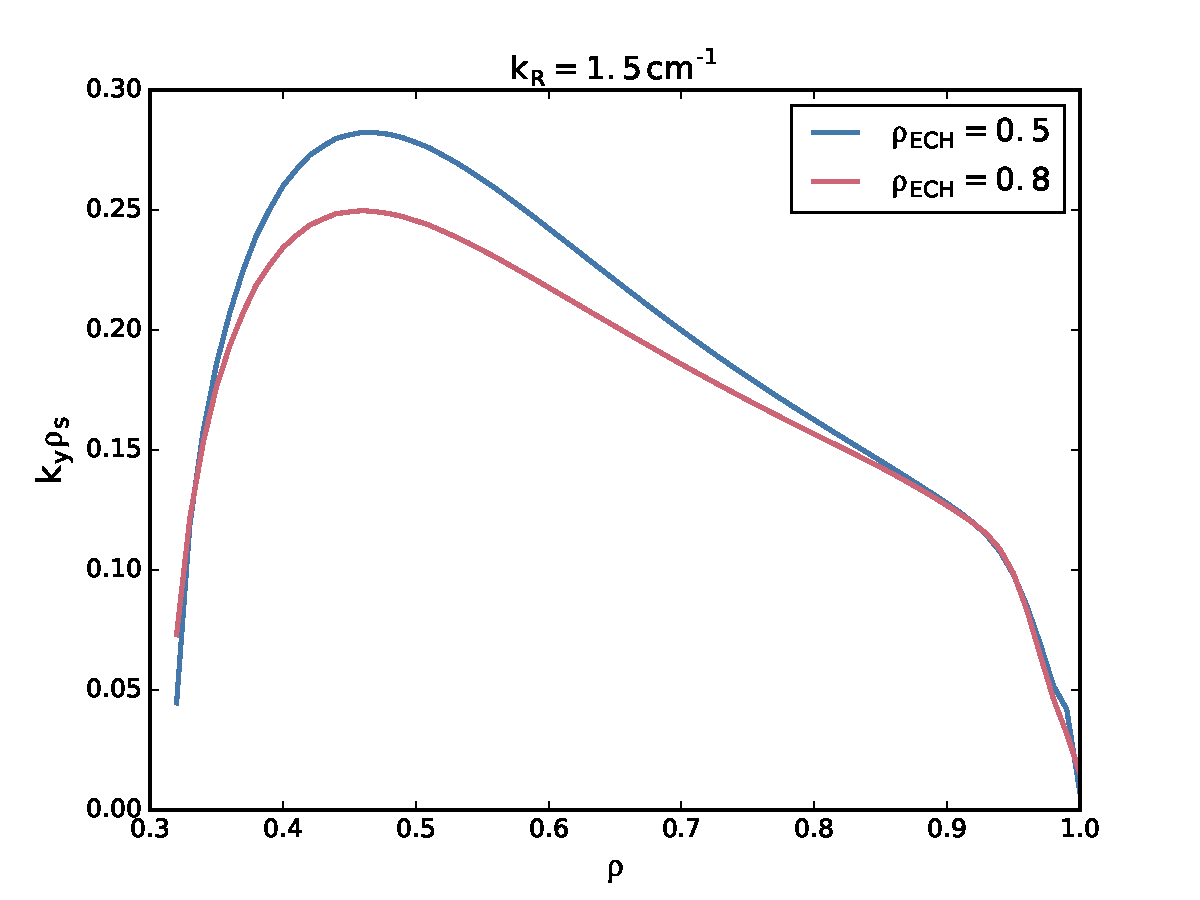
\includegraphics[width = \textwidth]{%
    Chapters/TurbulenceMeasurements/figs/wavenumber_conversion.pdf}
  \caption[Profiles of $k_y \rho_s$ for $k_R = \SI{1.5}{\per\centi\meter}$]{%
    Profiles of $|k_y \rho_s|$ vs.\ radial coordinate $\rho$ for
    the PCI low-$k$ cutoff $k_R = \SI{1.5}{\per\centi\meter}$,
    the interferometer high-$k$ cutoff $k_R = \SI{5}{\per\centi\meter}$, and
    the PCI high-$k$ cutoff $k_R = \SI{25}{\per\centi\meter}$
    in the $\rhoech = 0.5$ and $\rhoech = 0.8$ discharges
    shown in Figure~\ref{fig:TurbulenceMeasurements:profiles}.
    The gray region $(\rho \lesssim 0.35)$
    is inaccessible to the PCI probe beam,
    which propagates vertically through the plasma
    at major radius $R = \SI{1.98}{\meter}$.
    The roll-off in $|ky \rho_s|$ for $\rho \lesssim 0.4$
    is attributable to the $\sin\theta$ major-radial projection, while
    the roll-off for $\rho \gtrsim 0.95$
    is attributable to the edge pedestal.
  }
\label{fig:TurbulenceMeasurements:wavenumber_conversion}
\end{figure}


\subsection{Comparison to PCI-measured phase velocities}
\label{sec:TurbulenceMeasurements:Modeling:phase_velocity_comparison}
In an attempt to localize analysis of the TGLF results,
the advection of the TGLF-predicted instabilities by the $\ExB$ velocity
can be compared to the PCI-measured phase velocities.
The PCI-measured phase velocity is
\begin{equation}
  \vphpci
  =
  \frac{\omegapci}{k_R}
  =
  \frac{\kpci \cdot \vect{v}}{k_R},
  \label{eq:TurbulenceMeasurements:vphpci_general}
\end{equation}
where $\omegapci$ is the PCI-measured angular frequency,
$\kpci$ is the wavevector (\ref{eq:TurbulenceMeasurements:kpci_explicit}),
$\vect{v}$ is the lab-frame velocity of the fluctuation, and
$k_R$ is the reconstructed major-radial wavenumber
(\ref{eq:TurbulenceMeasurements:kR}).
By field-aligned constraint
(\ref{eq:TurbulenceMeasurements:kpci_perp_to_B0}),
$\kpci \cdot \vect{v} = \kpci \cdot \vperp$, where
$\vperp$ is the velocity
perpendicular to the equilibrium magnetic field.
The perpendicular velocity $\vperp$ is simply the sum of
the $\ExB$ velocity $\vExB$ and
the plasma-frame phase velocity
$\vect{v}_{\text{ph}}^{\text{plasma}}$ of the fluctuation;
here, the plasma-frame phase velocity is approximated
by that of the dominant wavevector, i.e.\
$\vect{v}_{\text{ph}}^{\text{plasma}} \approx \vphplasma \kzerohat$,
where $\kzerohat = \vect{k}_0 / |\vect{k}_0|$ and
$\vect{k}_0$ is the dominant wavevector defined in
(\ref{eq:TurbulenceMeasurements:k0}).
Thus, $\vperp \approx \vExB + \vphplasma \kzerohat$, and
\begin{equation}
  \omegapci
  =
  \kpci \cdot \vperp
  \approx
  \kpci \cdot \vExB
  +
  (\kpci \cdot \kzerohat)
  \vphplasma.
  \label{eq:TurbulenceMeasurements:omegapci}
\end{equation}
Now, the electrostatic potential $\varphi = \varphi(\rho)$
is a flux function such that
the corresponding electric field is
$\vect{E} = -\nabla \varphi = E_r(\rho, \theta) \rhohat$.
The resulting $\ExB$ velocity is
\begin{align}
  \vExB
  =
  \frac{\vect{E} \times \Beq}{B_0^2}
  % \notag \\
  =
  \frac{E_r(\rho, \theta)}{B_0^2}
  \left(%
    B_{\theta} \zetahat
    -
    B_{\zeta} \thetahat
  \right).
  \label{eq:TurbulenceMeasurements:vExB}
\end{align}
Using
$\kpci$ from (\ref{eq:TurbulenceMeasurements:kpci_explicit}),
$\vExB$ from (\ref{eq:TurbulenceMeasurements:vExB}),
$\vect{k}_0$ from (\ref{eq:TurbulenceMeasurements:k0}),
$\omegapci$ from (\ref{eq:TurbulenceMeasurements:omegapci}),
$k_R$ from (\ref{eq:TurbulenceMeasurements:kR}), and
a bit of algebra,
the PCI-measured phase velocity
(\ref{eq:TurbulenceMeasurements:vphpci_general})
readily reduces to
\begin{equation}
  \vphpci
  =
  \left[%
    \frac{E_r(\rho, \theta)}{B_0}
    -
    \vphplasma
  \right]
  \left( \frac{B_0}{B_{\zeta,0}} \right)
  \sin\theta.
  \label{eq:TurbulenceMeasurements:vphpci}
\end{equation}
The sign convention for the plasma-frame phase velocity is such that
$\vphplasma > 0$ for electron modes and
$\vphplasma < 0$ for ion modes.
For physical intuition regarding this sign convention,
consider a region of the plasma with $E_r > 0$;
here, electron modes propagate against the $\ExB$ direction
(decreasing $\vphpci$ relative to the $\ExB$ contribution alone), and
ion modes propagate in the $\ExB$ direction
(increasing $\vphpci$ relative to the $\ExB$ contribution alone).
The $B_0 / B_{\zeta,0}$ multiplicative enhancement to $\vphpci$
results from $|k_R| < |\kpci|$
when the magnetic field is not solely toroidal, and
the $\sin\theta$ term
provides the major-radial projection
required by the constraint
(\ref{eq:TurbulenceMeasurements:kpci_perp_to_Z});
note that $\vphpci$ changes sign about the midplane ($\theta = 0$)
due to this major-radial projection.
As the spatially filtering mask
\cite{dorris_rsi09, dorris_phd}
was not used in this experiment,
the PCI measurements cannot be localized
to above or below the midplane, and
only the magnitude of $\vphpci$ will be considered here.
Figure~\ref{fig:TurbulenceMeasurements:predicted_pci_phase_velocities}
compares the magnitude of the predicted PCI phase velocity
from (\ref{eq:TurbulenceMeasurements:vphpci})
to the measured PCI phase velocities
from the annotated turbulent branches
in Figure~\ref{fig:TurbulenceMeasurements:Skf_pci} and
infers that this turbulence is localized to
$0.6 \leq \rho \leq 0.65$.

\begin{figure}
  \centering
  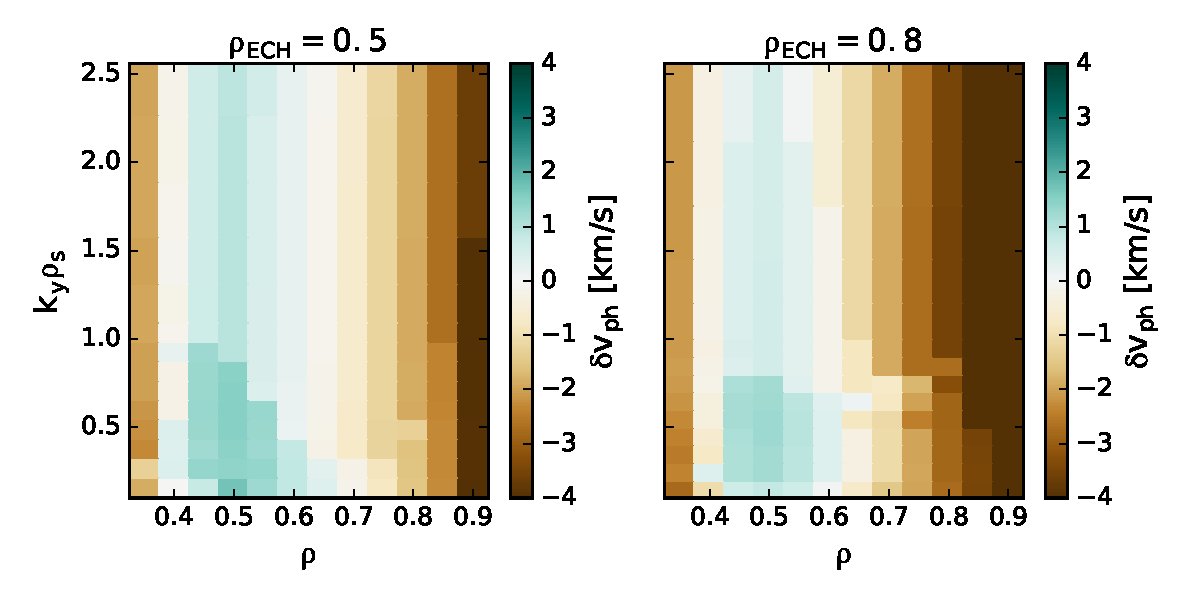
\includegraphics[width = \textwidth]{%
    Chapters/TurbulenceMeasurements/figs/predicted_pci_phase_velocities.pdf}
  \caption[Comparison of predicted and measured PCI phase velocities]{%
    Comparison of predicted and measured PCI phase velocities.
    Here, $\delta \vph$ is the difference between
    the predicted phase velocity and
    the measured phase velocity.
    The predicted phase velocity
    (\ref{eq:TurbulenceMeasurements:vphpci})
    is computed using
    the equilibrium profiles shown in
    Figure~\ref{fig:TurbulenceMeasurements:profiles} and
    the TGLF-predicted plasma-frame phase velocites shown in
    Figure~\ref{fig:TurbulenceMeasurements:linear_stability_overview}.
    The measured phase velocities correspond
    to the annotated turbulent branches in
    Figure~\ref{fig:TurbulenceMeasurements:Skf_pci}.
    The wavenumber range $k_y \rho_s$ considered here
    is restricted to $k_R \leq \SI{15}{\per\centi\meter}$,
    the maximum PCI-measured wavenumber in
    Fig~\ref{fig:TurbulenceMeasurements:Skf_pci}.
    The minimum discrepancy between
    the predicted and measured PCI phase velocities
    occurs between at $0.6 \leq \rho \leq 0.65$,
    suggesting that the annotated turbulent branches in
    Figure~\ref{fig:TurbulenceMeasurements:Skf_pci}
    are localized to $0.6 \leq \rho \leq 0.65$.
  }
\label{fig:TurbulenceMeasurements:predicted_pci_phase_velocities}
\end{figure}

As a brief aside, it should be emphasized
that the radial electric field $E_r$
in (\ref{eq:TurbulenceMeasurements:vphpci})
is \emph{not} a flux function.
To see this, recall that
the corresponding electrostatic potential
\emph{is} a flux function,
i.e.\ $\varphi = \varphi(\rho) = \varphi(\psi)$,
where $\psi$ is the flux-surface label
corresponding to the poloidal magnetic-field flux per radian.
Now,
\begin{align}
  E_r(\rho, \theta)
  &=
  -\left( \frac{\partial\varphi}{\partial r} \right)
  \notag \\
  &=
  -\left( \frac{d\varphi}{d\psi} \right)
  \left( \frac{\partial\psi}{\partial r} \right)
  \notag \\
  &=
  -\left( \frac{d\varphi}{d\psi} \right)
  \left( R B_{\theta} \right),
\end{align}
where the last line follows from the definition
of $\psi$ as the poloidal magnetic-field flux per radian.
The derivative $d\varphi / d\psi$
is a flux function because $\varphi$ is a flux function, and
this implies that $E_r / (R B_{\theta})$ is also a flux function.
Thus, the radial electric field at any point
within the last closed flux surface can be computed
from the radial electric field
along the outboard midplane (where $\theta = 0$) as follows
\begin{equation}
  \left.
  \frac{E_r}{R B_{\theta}}
  \right|_{\rho, \theta}
  =
  \left.
  \frac{E_r}{R B_{\theta}}
  \right|_{\rho, \theta = 0}.
  \label{eq:TurbulenceMeasurements:radial_electric_field}
\end{equation}


\subsection{Quantitative local results}
\label{sec:TurbulenceMeasurements:Modeling:local}
A global overview of the TGLF-predicted linear stability was presented in
Section~\ref{sec:TurbulenceMeasurements:Modeling:linear_stability_overview}.
In Section~\ref{sec:TurbulenceMeasurements:Modeling:phase_velocity_comparison},
the annotated turbulent branches
from Figure~\ref{fig:TurbulenceMeasurements:Skf_pci}
were localized to $0.6 \leq \rho \leq 0.65$.
Thus, it is now reasonable
to perform a more quantitative assessment
of the corresponding local TGLF predictions.
Below, TGLF predictions are shown for $\rho = 0.6$, but
comparable predictions are made at $\rho = 0.65$.

Figure~\ref{fig:TurbulenceMeasurements:linear_stability_local}
displays the TGLF-predicted linear stability
at radial location $\rho = 0.6$
for $\rhoech = 0.5$ and $\rhoech = 0.8$.
Both operational scenarios are predicted
to destabilize ion and electron modes
across multiple spatiotemporal scales, but
$\rhoech = 0.5$ is predicted
to destabilize a continuum
of mid-$k$ ($0.5 \lesssim k_y \rho_s \lesssim 5$) electron modes
that bridge the gap between
low-$k$ ($k_y \rho_s \lesssim 0.5$) ion modes and
high-$k$ ($k_y \rho_s \gtrsim 5$) electron modes,
potentially facilitating cross-scale coupling.
Further, relative to $\rhoech = 0.8$,
the $\rhoech = 0.5$ ion-mode growth rates
are substantially reduced
(becoming comparable to the $\ExB$ shearing rate
shown in Figure~\ref{fig:TurbulenceMeasurements:profiles}(h)), and
the high-$k$ electron-mode growth rates
are marginally enhanced,
both of which may also facilitate cross-scale coupling.

\begin{figure}
  \centering
  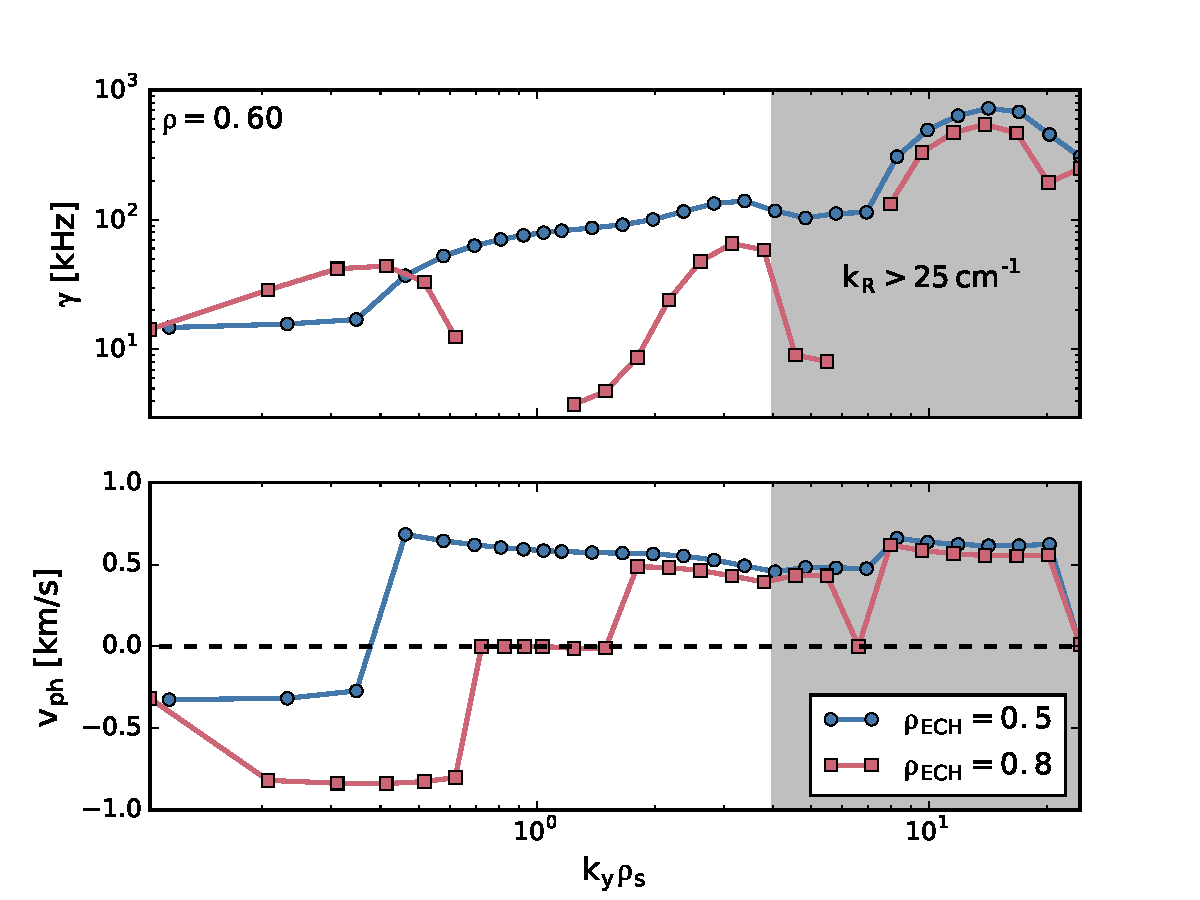
\includegraphics[width = \textwidth]{%
    Chapters/TurbulenceMeasurements/figs/linear_stability_local.pdf}
  \caption[TGLF-predicted linear stability at $\rho = 0.6$]{%
    TGLF-predicted linear stability at $\rho = 0.6$
    for the profiles shown in
    Figure~\ref{fig:TurbulenceMeasurements:profiles}.
    Linear growth rates $\gamma$ and
    plasma-frame phase velocities $\vph = \omega / k_y$
    are plotted as a function of
    normalized fluctuation wavenumber $k_y \rho_s$
    for $\rhoech = 0.5$ and $\rhoech = 0.8$.
    Electron modes have $\vph > 0$, and
    ion modes have $\vph < 0$.
    The gray region exceeds the spatial bandwidth
    of the combined PCI-interferometer
    developed in this work.
    Growth rates can be compared
    to the $\ExB$ shearing rates $\gamma_E$
    in Figure~\ref{fig:TurbulenceMeasurements:profiles}(h).
  }
\label{fig:TurbulenceMeasurements:linear_stability_local}
\end{figure}

Howard \emph{et al.} suggest a linear-stability ``rule of thumb''
for gauging the importance of cross-scale coupling~\cite{howard_pp16}.
The rule of thumb attempts to quantify the relative ``strength''
of electron-scale to ion-scale turbulence
by examining the ratio of
the maximum electron-scale growth rate $\gammahighk$ to
the maximum ion-scale growth rate $\gammalowk$,
with larger values of $\gammahighk / \gammalowk$
corresponding to increased cross-scale coupling.
Howard \emph{et al.} constrain their search
for $\gammahighk$ to $2 \leq k_y \rho_s \leq 48$ and
for $\gammalowk$ to $0.25 \leq k_y \rho_s \leq 0.75$.
For consistency, this same selection criterion is used below.
For $\rhoech = 0.8$,
Figure~\ref{fig:TurbulenceMeasurements:linear_stability_local} shows that
$\gammahighk = \SI{540}{\kilo\hertz}$ at $k_y \rho_s = 14$ and
$\gammalowk = \SI{43}{\kilo\hertz}$ at $k_y \rho_s = 0.4$ such that
$\gammahighk / \gammalowk = 12.6$;
with such a small value,
the rule of thumb suggests that cross-scale coupling
is insignificant.
For $\rhoech = 0.5$,
Figure~\ref{fig:TurbulenceMeasurements:linear_stability_local} shows that
$\gammahighk = \SI{720}{\kilo\hertz}$ at $k_y \rho_s = 14$ and
$\gammalowk = \SI{63}{\kilo\hertz}$ at $k_y \rho_s = 0.7$ such that
$\gammahighk / \gammalowk = 11.4$,
less than the $\rhoech = 0.8$ case.
It should be noted, however,
that the distinct mid-$k$ electron branch
in Figure~\ref{fig:TurbulenceMeasurements:linear_stability_local}
is \emph{absent} from the plasmas
used to develop the rule of thumb;
further, the above $\gammalowk$ for $\rhoech = 0.5$
corresponds to this mid-$k$ electron branch.
If $\gammalowk$ is instead restricted to an ion mode,
$\gammalowk = \SI{17}{\kilo\hertz}$ at $k_y \rho_s = 0.35$ such that
$\gammahighk / \gammalowk = 42$;
cross-scale coupling can be important in ELMy H-mode plasmas
with this $\gammahighk / \gammalowk$~\cite{howard_ppcf18}.

In addition to assessing linear stability,
TGLF can predict the electron-density fluctuation spectrum
using quasilinear transport and
a model for the nonlinear saturation of the turbulence.
This saturation model is fit to results
from nonlinear gyrokinetic simulations~\cite{staebler_pp07},
the most recent of which include
realistic multiscale physics~\cite{staebler_nf17}.
The multiscale saturation model is referred to as SAT$1$.
The density fluctuation spectrum
predicted by TGLF-SAT$1$ at $\rho = 0.6$
is shown Figure~\ref{fig:TurbulenceMeasurements:density_spectra_local}.
Within the PCI sensitivity and wavenumber domain,
the predicted spectra are qualitatively consistent
with the PCI-measured spectra
in Figure~\ref{fig:TurbulenceMeasurements:Sk_power_law}.
Specifically, the $\rhoech = 0.5$ spectrum
is noticeably flatter (i.e.\ decays more slowly)
than the $\rhoech = 0.8$ spectrum, which
may be indicative of enhanced cross-scale coupling~\cite{howard_pp16}.
Further, the intersection of the two predicted spectra
is in rough agreement
with that observed in the PCI-measured spectra.
However, the predicted and measured power laws
quantitatively disagree.
It should be emphasized that the TGLF-SAT$1$ model
is fit to just a handful~\cite{staebler_nf17}
of realistic multiscale gyrokinetic simulations
corresponding to Alcator C-Mod L-mode plasmas, so
quantitative agreement may improve
when additional multiscale simulations are completed and
the TGLF-SAT$1$ model is recalibrated.

\begin{figure}
  \centering
  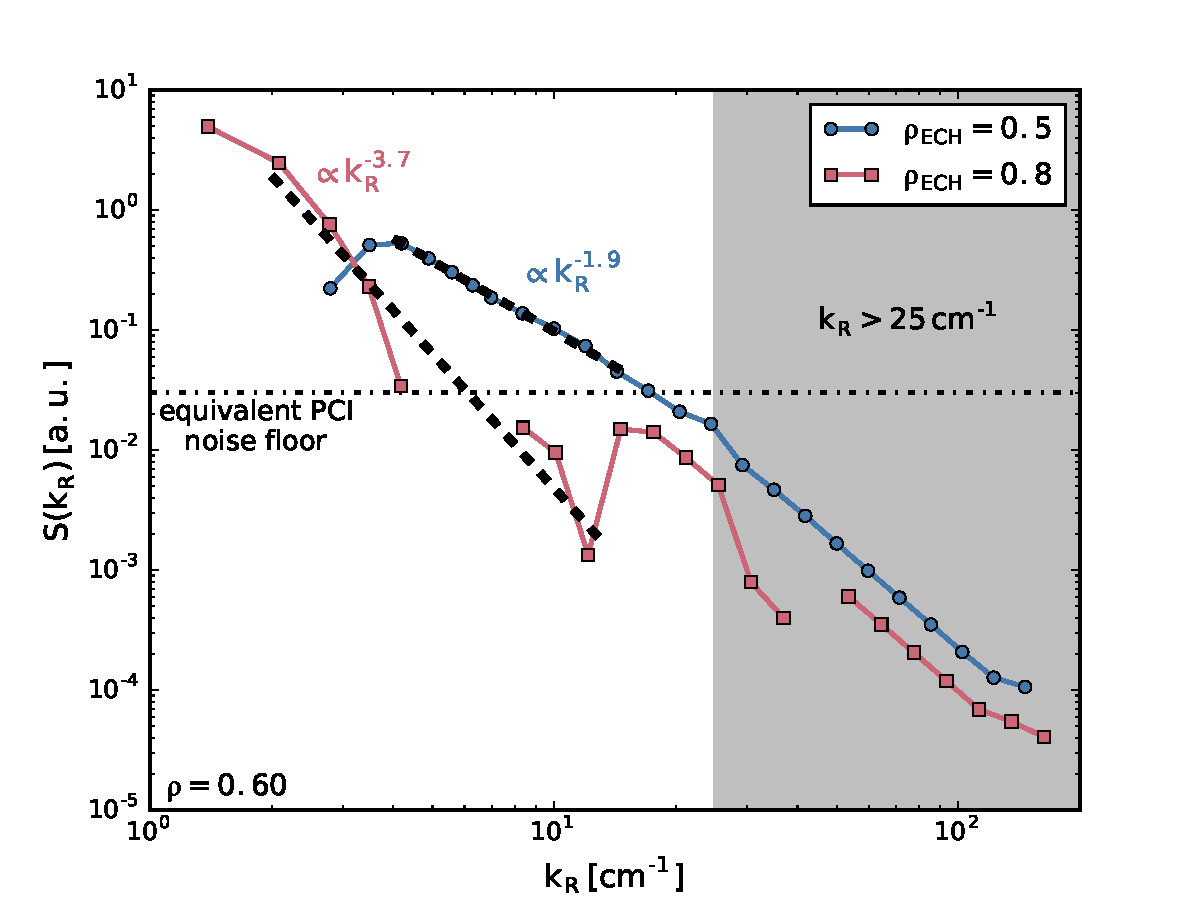
\includegraphics[width = \textwidth]{%
    Chapters/TurbulenceMeasurements/figs/density_spectra_local.pdf}
  \caption[TGLF-predicted electron-density fluctuation spectra]{%
    Electron-density fluctuation spectra
    predicted by TGLF-SAT$1$
    at radial location $\rho = 0.6$
    for $\rhoech = 0.5$ and $\rhoech = 0.8$.
    The gray region exceeds the spatial bandwidth
    of the combined PCI-interferometer
    developed in this work.
    The equivalent PCI noise floor,
    indicated by the horizontal dash-dot line,
    is inferred from the noise floor
    in Figure~\ref{fig:TurbulenceMeasurements:Sk_power_law};
    that is, for $\rhoech = 0.5$
    the equivalent noise floor intersects $S(k_R)$
    at $k_R \approx \SI{15}{\per\centi\meter}$,
    which is roughly equivalent to the $\rhoech = 0.5$ noise floor
    in Figure~\ref{fig:TurbulenceMeasurements:Sk_power_law}.
    Within the PCI sensitivity and wavenumber domain,
    the predicted spectra are qualitatively consistent
    with the PCI-measured spectra
    in Figure~\ref{fig:TurbulenceMeasurements:Sk_power_law}.
    The black dashed lines indicate least-squares power-law fits
    to the predicted $S(k_R)$;
    the resulting power laws quantitatively disagree
    with the PCI-measured power laws in
    Figure~\ref{fig:TurbulenceMeasurements:Sk_power_law}.
  }
\label{fig:TurbulenceMeasurements:density_spectra_local}
\end{figure}


\bibliographystyle{plainurl}
\bibliography{references}
%
\chapter{Conclusions \& future work}
\label{ch:Conclusions}


\section{Summary \& conclusions}
\label{sec:Conclusions:summary_and_conclusions}
The work described in this thesis can be summarized as follows:
\begin{itemize}
  \item Chapter~\ref{ch:InterferometricMethods} discusses
    the theory of optical interferometric methods
    in the context of measuring tokamak plasma-density fluctuations.
    The laser-plasma interaction is quantified via
    Fraunhofer scalar-diffraction theory, and
    the resulting diffracted field is imaged onto a square-law detector.
    Interfering the imaged field with a known reference field
    produces measurable intensity fluctuations;
    the specification of this reference field
    defines the interferometric method.
    Details of two particular interferometric methods ---
    external-reference-beam interferometry and
    phase contrast imaging (PCI) ---
    are discussed, with an emphasis on
    their sensitivity to fluctuations and their spatiotemporal bandwidths.
    Significantly, while PCI can measure fluctuations more sensitively
    than an external-reference-beam interferometer,
    PCI suffers from a low-$k$ cutoff;
    an external-reference-beam interferometer
    does \emph{not} suffer from such a low-$k$ cutoff.
  \item Chapter~\ref{ch:DesignConsiderations} considers the design of an
    external-reference-beam, heterodyne interferometer
    (hereafter referred to as a heterodyne interferometer).
    A criterion for satisfactory wavefront matching
    between the probe beam and the reference beam is developed, and
    finite-sampling-volume effects are shown
    to constrain the heterodyne interferometer's spatial bandwidth.
    The effects of phase noise, amplitude noise, and digitizer bit noise
    are each discussed in the context of
    the heterodyne interferometer's signal-to-noise ratio, and
    the systematic errors resulting from
    imperfect demodulation of the heterodyne interference signal
    are quantified.
  \item Chapter~\ref{ch:Implementation} details
    the addition of a heterodyne interferometer
    to the pre-existing PCI system on the \diiid\space tokamak.
    Both systems operate simultaneously,
    sharing a single $\SI{10.6}{\micro\meter}$ probe beam through the plasma.
    Optical-diagnostic access on \diiid\space and the capabilities
    of the pre-existing PCI system are briefly reviewed.
    Referencing the design considerations
    in Chapter~\ref{ch:DesignConsiderations} and
    adopting the philosophy
    that the pre-existing PCI system should be minimally perturbed,
    the optical layout for the heterodyne interferometer is developed;
    the magnification of the interferometer's imaging system
    is selected such that the spatial bandwidths
    of the PCI and interferometer have a mid-$k$ overlap.
    The design, procurement, and installation
    of the new optical and electrical components
    required to make the heterodyne interferometric measurement
    are summarized.
    Of note is the interferometer's radio-frequency local oscillator:
    the phase noise of a crystal oscillator (XO)
    was empirically found to be \emph{too large}
    to make meaningful fluctuation measurements in most tokamak plasmas, but
    the substantially lower phase noise of an
    oven-controlled crystal oscillator (OCXO)
    allows measurements of a whole zoo
    of coherent and broadband plasma fluctuations.
    The interferometer response and
    the multiscale capabilities of the combined PCI-interferometer
    are empirically verified via sound-wave calibrations.
    Specifically, the PCI is shown to measure high-$k$
    ($\SI{1.5}{\per\centi\meter} < |k_R| \leq \SI{25}{\per\centi\meter}$)
    fluctuations with
    sensitivity $3 \times 10^{13} \; \text{m}^{-2} / \sqrt{\text{kHz}}$,
    while the interferometer simultaneously measures low-$k$
    ($|k_R| < \SI{5}{\per\centi\meter}$) fluctuations with
    sensitivity $3 \times 10^{14} \; \text{m}^{-2} / \sqrt{\text{kHz}}$.
    Both systems have temporal bandwidths in excess of $\SI{1}{\mega\hertz}$.
  \item Chapter~\ref{ch:ToroidalCorrelation} discusses the correlation
    of the newly installed interferometer with
    \diiid's toroidally separated, pre-existing $V2$ interferometer.
    Capable of probing the core plasma,
    the interferometers are shown to be sensitive
    to core-localized fluctuations
    that are \emph{invisible} to external magnetic probes.
    The chapter begins with a brief review
    of the two-point correlation technique and
    shows how toroidal mode numbers can be extracted
    from a pair of toroidally separated measurements.
    Meaningful correlation requires that
    the two measurements share the same timebase.
    The digitizers of both interferometers were modified
    to phase lock their clocks, and
    a residual ``trigger offset'' was measured
    and is compensated in software.
    Where comparisons can be made with magnetic probes,
    the interferometer-measured toroidal mode numbers
    are in good agreement.
    Currently, there is not a tested, robust method
    for correcting the bias introduced by
    the $\SI{4}{\centi\meter}$ major-radial offset
    between the interferometer beam centers,
    which unfortunately limits the
    deployment of this system for physics studies
    of core-localized MHD.
  \item Chapter~\ref{ch:TurbulenceMeasurements} demonstrates
    the multiscale capabilities of the combined PCI-interferometer.
    During a recent \diiid\space experiment,
    the location of electron cyclotron resonance heating (ECH)
    was moved from $\rhoech = 0.5$ to $\rho_{ECH} = 0.8$,
    altering the local $a / L_{T_e}$ and $a / L_{T_i}$
    in an attempt to change the coupling between
    the electron-scale and ion-scale turbulence.
    As such, this experiment presents an ideal opportunity
    for multiscale turbulence investigations
    with the combined PCI-interferometer.
    Numerous turbulent branches are observed.
    In particular, the interferometer measures
    a low-$k$ electromagnetic mode driven unstable by collisionality,
    properties consistent with the micro-tearing mode (MTM), and
    the PCI measures a wavenumber spectrum
    that exhibits distinct flattening
    when $a / L_{T_e}$ is increased relative to $a / L_{T_i}$,
    reminiscent of results
    from realistic multiscale gyrokinetic simulations~\cite{howard_pp16}.
    To aid the interpretation of these measurements,
    linear-stability analysis and quasilinear-transport modeling
    are performed with the gyro-Landau fluid code TGLF, and
    qualitative agreement with the PCI-measured wavenumber spectrum
    is obtained.
\end{itemize}


\section{Future work}
\label{sec:Conclusions:future_work}
The combined PCI-interferometer developed in this work
has a clear application in the burgeoning study
of multiscale turbulence and cross-scale coupling, which
may be significant in the reactor relevant $T_e \approx T_i$ regime.
In roughly the next six months,
Howard \emph{et al.} expects to complete
realistic multiscale gyrokinetic simulations
for the experiment described in
Chapter~\ref{ch:TurbulenceMeasurements}.
It will be very interesting
to see if the predicted wavenumber spectrum
matches the PCI-measured wavenumber spectrum.
It should be noted that a synthetic PCI diagnostic
already exists for the interpretation
of such gyrokinetic simulations~\cite{rost_pp10}.
Small modifications to the synthetic PCI
should also allow a synthetic interferometer diagnostic.
Previous multiscale simulations predict
significant local and non-local energy cascades
between the ion and electron scales~\cite{howard_pp16}, so
it is desirable to investigate such coupling empirically.
With its large spatiotemporal bandwidth,
the combined PCI-interferometer may be ideally suited
for measurement of such coupling, which
may be suitably quantified by
the bicoherence~\cite{young_and_powers_ieee79}
between various channels of the system or
some other suitable measure of nonlinear processes.
(Note that the author has performed preliminary bispectral analysis
of the measurements discussed in
Chapter~\ref{ch:TurbulenceMeasurements};
interestingly, the $|k_R| \sim \SI{5}{\per\centi\meter}$ and
$f \sim \SI{1}{\mega\hertz}$ mode observed in
Figure~\ref{fig:TurbulenceMeasurements:Skf_pci}(b)
has an exceptionally large autobicoherence).

The interferometer-measured, low-$k$, electromagnetic modes
that are destabilized by collisionality
are also deserving of further study.
The properties of this mode are consistent
with the micro-tearing mode, which
was predicted to be marginally unstable
in the multiscale experiment's reference discharge~\cite{holland_nf17}.
Unfortunately, TGLF's default eigenfunction basis
of four Hermite polynomials is typically insufficient
to resolve micro-tearing modes (MTMs)~\cite{staebler_MTM_question}, so
there are no attempts to simulate the MTM in this work.
However, it may be conceivable that
increasing the number of Hermite polynomials
will allow identification of the MTM in TGLF.
Alternatively, linear simulations with
the gyrokinetic code GYRO~\cite{candy_jcp03}
could be pursued.
(Note that the reference-discharge simulations
indicating marginal MTM instability were performed with GYRO).
Experimentally, it is desirable to map out the parametric dependencies
of this mode, particularly its response
to the plasma $\beta$ and collisionality.
If dedicated experiments cannot be performed,
it should be noted that the relevant experimental conditions
(i.e.\ ITER-baseline scenario) are fairly typical at \diiid, and
a fair amount may still be learned
by ``piggybacking'' on other experiments.

With regards to the combined PCI-interferometer,
the most substantial improvement to the system
would be upgrading the heterodyne-interferometer detector
from a single element to a multi-element array.
This would allow reconstruction of $k_R$
from the interferometer measurements,
enabling estimates of
frequency-wavenumber spectra $S_{\phi,\phi}(k,f)$ and
wavenumber spectra $S_{\phi,\phi}(k)$
much like with the PCI.
This capability is desirable for several reasons.
First and foremost,
interferometric measurements across a multi-element array
would allow accurate estimates of $S_{\phi,\phi}(k)$
below the PCI low-$k$ cutoff
(\ref{eq:Implementation:kg_realized}), which
may have important implications for
validation of spectral-flattening predictions
from multiscale gyrokinetic predictions.
Further, as discussed in
Section~\ref{sec:Implementation:Calibration:pci},
interferometric measurements across a multi-element array
would allow robust and accurate
cross-calibration of the PCI
on a shot-to-shot and an intra-shot basis.
Note that each additional detector element
would require its own set of electronics
(e.g.\ signal conditioning RF amplifiers,
demodulation electronics, and
audio amplifiers) and
two additional digitizer channels
(to digitize both the in-phase $I$ and quadrature $Q$ signals).
While the ``deadbug'' circuit construction utilized in this work
is ideal for prototyping,
any future increase to the number of interferometer channels
would call for a printed-circuit-board (PCB) construction
of the electronics.
Thus, increasing the number of interferometer channels
is not a small undertaking.

A simpler, cheaper, and faster performance improvement
would be the procurement of anti-aliasing filters
with a higher cutoff frequency.
The current anti-aliasing filters
limit the bandwidth of the interferometer to
approximately $\SI{1}{\mega\hertz}$, but
the upstream components have bandwidths
in excess of $\SI{2}{\mega\hertz}$.
Thus, new anti-aliasing filters could,
quite literally overnight,
nearly double the temporal bandwidth of the interferometer.

Finally, there is not currently a tested, robust method
for correcting the bias introduced by
the major-radial offset of the toroidally correlated interferometers
(other than reducing the offset, i.e.\ $\Delta R \rightarrow 0$,
which is not possible with current port allocations).
It may be possible to account for the radial and poloidal mode structure
via e.g.\ measurements from
microwave imaging reflectometry (MIR)~\cite{muscatello_rsi14} or
electron cyclotron emission imaging (ECEI)~\cite{tobias_rsi10}.

Looking towards ITER and other next-step devices,
the combined PCI-interferometer may allow
sensitive, high spatiotemporal bandwidth measurements
of multiscale turbulence.
The diagnostic development pursued in this thesis
proves that heterodyne-interferometric detection and PCI detection
can be simultaneously implemented
using a shared probe beam and
a shared set of ports.
The addition of PCI detection to
e.g.\ the ITER interferometer~\cite{vanzeeland_TIP_rsi13}, however,
is not without its challenges.
For example, the ITER interferometer
employs a Michelson configuration,
with the beam making a second pass through the plasma
after bouncing off of a retroreflector inside the vacuum vessel.
In contrast,
at least to the author's knowledge,
all previous PCI implementations
have employed a Mach-Zehnder configuration,
with the probe beam making a single pass through the plasma.
In principle, PCI can use a Michelson configuration, but
the double pass and retroreflector
may complicate interpretation of the measurements,
particularly if attempting to localize the measurements
with a spatially filtering mask~\cite{dorris_rsi09, dorris_phd, lin_rsi06} or
with $2$-dimensional detector arrays~\cite{sanin_rsi04, tanaka_rsi16}.

Regardless, the spatial bandwidth of a PCI system
that shares its probe beam
with the ITER interferometer can be considered.
The 1/e $E$ waist of the ITER interferometer's
$\SI{10.6}{\micro\meter}$ probe beam is
$w_0 \approx \SI{8}{\milli\meter}$~\cite{vanzeeland_TIP_rsi13}
such that a PCI system using this probe beam
would have a diffraction-limited low-$k$ cutoff
(\ref{eq:InterferometricMethods:pci_kmin_physics})
of $\SI{2.5}{\per\centi\meter}$.
(However, recall that the \diiid\space PCI
is operated two to three times above the diffraction limit
to give some leeway to the PCI feedback system).
Of course, as demonstrated in this thesis,
simultaneous heterodyne-interferometric and PCI detection
can obviate the PCI's low-$k$ cutoff.
A somewhat larger problem, however, may be the limited collection volumes
and long path lengths
between the vacuum vessel and the detector, which
may impose severe constraints
on the high-$k$ cutoff of a $\SI{10.6}{\micro\meter}$ PCI or interferometer.
One potential solution is to use a smaller probe wavelength
(i.e.\ larger $k_0$) to decrease the scattering angle $\theta_m$ from
(\ref{eq:GaussianBeamDiffraction:scattering_angles}).
As the burning plasma regime will be predominantly electron heated
(i.e.\ via fusion alpha particles slowing down on electrons),
it is extremely important that
both high-$k$ electron turbulence and
any cross-scale coupling with low-$k$ ion turbulence
is accurately diagnosed and understood.


\bibliographystyle{plainurl}
\bibliography{references}
%


% **********
% Backmatter
% **********
\appendix%
\cleardoublepage%
\chapter{Diffraction of a Gaussian probe beam}
\label{app:GaussianBeamDiffraction}


\section{Kirchhoff scalar-diffraction theory}
As discussed in the text surrounding
(\ref{eq:InterferometricMethods:electric_field_eigenvector}),
a CO$_2$ probe beam in a tokamak plasma propagates
as a transverse electromagnetic wave with near-constant polarization
(with any small changes to beam polarization being
of little practical interest to the present work).
Thus, it is suitable to pursue a \emph{scalar} theory
of the beam's interaction with the plasma.
Below, Kirchoff's scalar-diffraction theory is summarized.

A monochromatic scalar wave $U(\vect{r}) e^{-i \omega t}$ in vacuum
satisfies the Helmholtz equation
\begin{equation}
  (\nabla^2 + k^2) U = 0,
\end{equation}
where $k = \omega / c$.
The Helmholtz-Kirchhoff integral theorem states
that the field at a point $P$ is
\begin{equation}
  U(P)
  =
  \frac{1}{4 \pi}
  \int_S \left[
    U \frac{\partial}{\partial n}\left(\frac{e^{i k s}}{s}\right)
    -
    \frac{e^{i k s}}{s} \frac{\partial U}{\partial n}
  \right] dS,
  \label{eq:GaussianBeamDiffraction:Helmholtz_Kirchhoff_integral_theorem}
\end{equation}
where $S$ is an arbitrary surface that encloses $P$,
$\vect{s}$ is the vector from point $P$ to differential area element $dS$,
$\vect{n}$ is the \emph{inward}-pointing normal of surface $S$, and
$U$ is assumed to be differentiable to second order within and on $S$
\cite[Sec.~8.3]{born_and_wolf}.
The relevant geometry is sketched
in Fig.~\ref{fig:GaussianBeamDiffraction:Kirchhoff_geometry}(a).

\begin{figure}
  \centering
  \includegraphics[width = \textwidth]{%
    Appendices/GaussianBeamDiffraction/figs/kirchhoff_geometry.eps}
  \caption[Geometries for Kirchhoff diffraction calculations]{%
    Geometries for Kirchhoff scalar-diffraction calculations.
    When $S_1$ is imaged by an optical system,
    $S_1$ is referred to as the \emph{object plane}.}
\label{fig:GaussianBeamDiffraction:Kirchhoff_geometry}
\end{figure}

To proceed with the diffraction calculation,
assume that the incident waves propagate in the $+z$-direction and
adopt the surface drawn
in Fig.~\ref{fig:GaussianBeamDiffraction:Kirchhoff_geometry}(b).
That is, $S = S_1 + S_2$,
where $S_1$ is a circle in the $(x, y)$-plane, and
$S_2$ is a spherical segment centered on the optical axis.
When $S_1$ is imaged by an optical system,
$S_1$ is referred to as the \emph{object plane}.
Now, assume that the incident waves were ``turned on''
at some finite time in the past, and
take the radius of $S_2$ to be large enough such that
none of the diffracted waves have had sufficient time to reach $S_2$,
i.e.\ $U \equiv 0$ on $S_2$.
(Of course, strictly speaking, the source's finite turn-on time
requires relaxation of the monochromatic assumption.
Finite turn-on time does not preclude a pseudo-monochromatic source, however,
and such a source is assumed hereafter).
Thus, the integral over $S_2$ vanishes, and
the diffraction calculation reduces to an integral over $S_1$.

Now, evaluation of
the Helmholtz-Kirchhoff integral
(\ref{eq:GaussianBeamDiffraction:Helmholtz_Kirchhoff_integral_theorem})
requires knowledge of $U$ on $S_1$.
For free-space propagation,
$S_1$ is an imagined (rather than a physical) surface
that does not impede the propagation of the incident wave $U^{(i)}$
(that is, $U = U^{(i)}$ and
$\partial U / \partial n = \partial U^{(i)} / \partial n$ on $S_1$).
If, however, $S_1$ contains opaque obstacles,
the free-space propagation conditions are no longer valid;
instead, the Kirchhoff boundary conditions can be adopted:
\begin{align}
  \text{surfaces of clear aperture:}&
  \quad
  U = U^{(i)},
  \quad
  \frac{\partial U}{\partial n} = \frac{\partial U^{(i)}}{\partial n},
  \notag \\
  \text{opaque surfaces:}&
  \quad \;
  U = 0,
  \qquad
  \frac{\partial U}{\partial n} = 0.
  \notag
\end{align}
While these boundary conditions are adequate for the current application,
it should be noted that they are not physical
for points that are very close to the boundaries of the opaque obstacles.


\section{Free-space diffraction of a Gaussian beam}
This section demonstrates that the Fraunhofer diffraction formalism
gives the correct form for a free-space Gaussian beam in the far-field limit,
and it also lays the groundwork for examining
the diffraction of a Gaussian beam from plasma-density fluctuations.
Note that the Gaussian-beam definition provided in
Section~\ref{sec:InterferometricMethods:Gaussian_beam_diffraction:Gaussian_beam_definition}
is used throughout the remainder of this appendix.

Assume that the incident Gaussian beam has a waist at $S_1$, and
take the radius of $S_1$ to be much larger than the beam waist $w_0$
such that the domain of integration effectively extends
over the whole $(x, y)$-plane.
For free-space propagation,
$S_1$ does not perturb the Gaussian beam; thus,
$E(\vect{r}, t) = E^{(i)}(\vect{r}, t) = E_G(\vect{r}) e^{-i \omega_0 t}$,
where $E_G(\vect{r})$ is the Gaussian beam's spatial dependence,
as defined by (\ref{eq:InterferometricMethods:Gaussian_beam}).
Now, in the far-field ($k_0 s \gg 1$) and
paraxial ($\vect{s} \approx -z \hat{\vect{z}}$) approximations
\begin{align}
  \left. \frac{e^{i k_0 s}}{s} \right|_{S_1}
  &\approx
  \frac{e^{i k_0 s}}{z},
  \notag \\
  \left. \frac{\partial}{\partial n}
  \left( \frac{e^{i k_0 s}}{s} \right) \right|_{S_1}
  &\approx
  -i k_0 \left( \frac{e^{i k_0 s}}{z} \right).
  \notag
\end{align}
The $s$-dependence in the phase arguments has been retained,
as it is the mechanism responsible for diffraction, but
the $s$-dependence in the amplitude has been dropped
as it only gives rise to negligible variations
in the amplitude of the diffracted wave.
Relative to a spherical wave,
a Gaussian beam has several additional $z$-dependencies;
however, at the beam's waist
\begin{align}
  \left. \frac{\partial w(z)}{\partial z} \right|_{\text{waist}}
  &\equiv
  0,
  \notag \\
  \left. \frac{\partial}{\partial z}
  \left[ \frac{1}{R(z)} \right] \right|_{\text{waist}}
  &=
  \frac{1}{z_R^2},
  \notag \\
  \left. \frac{\partial \psi(z)}{\partial z} \right|_{\text{waist}}
  &=
  \frac{1}{z_R}.
  \notag
\end{align}
Then, if the beam's Rayleigh range is much greater than
the probe wavelength ($k_0 z_R \gg 1$) and
the relevant transverse dimensions are much less than
the Rayleigh range ($w_0 \ll z_R$),
the Gaussian beam at $S_1$ satisfies
\begin{align}
  \left. E_G(\vect{r}') \right|_{S_1}
  &\approx
  E_0 e^{-(\rho' / w_0)^2},
  \notag \\
  \left. \frac{\partial E_G(\vect{r}')}{\partial n} \right|_{S_1}
  &\approx
  i k_0 \left[ E_0 e^{-(\rho' / w_0)^2} \right].
  \notag
\end{align}
Note that the CO$_2$ laser beams ($k_0 \approx \SI{2 \pi e5}{\per\meter}$)
that probe tokamak plasmas often have $z_R \gg \SI{10}{\meter}$
such that $k_0 z_R \gg 1$ and $w_0 \ll z_R$
(the transverse dimensions are constrained by the machine size
such that $w_0 \ll \SI{1}{\meter}$) are very well-satisfied.

Substituting the above expressions for
the incident waves and their surface-normal derivatives into
the Helmholtz-Kirchhoff integral
(\ref{eq:GaussianBeamDiffraction:Helmholtz_Kirchhoff_integral_theorem})
and simplifying yields
\begin{equation}
  E(\vect{r})
  \approx
  \frac{-i E_0}{\lambda_0 z}
  \int_{S_1}
  e^{-( \rho' / w_0 )^2}
  e^{i k_0 s}
  dS.
  \label{eq:GaussianBeamDiffraction:Kirchhoff_diffraction_integral}
\end{equation}
To proceed further, $s$ must be approximated:
\begin{align}
  s
  &=
  | \vect{\rho}' - \vect{r}|
  \notag \\
  &=
  \left[ r^2 - 2(x'x + y'y) + (x'^2 + y'^2) \right]^{1/2}
  \notag \\
  &\approx
  r - \frac{x'x + y'y}{r},
  \label{eq:GaussianBeamDiffraction:Fraunhofer_s}
\end{align}
where only terms linear in $(x' / r)$ and $(y' / r)$ have been retained.
This is known as the Fraunhofer limit, and
it is valid in the far-field $z \gg z_R$~\cite[Sec.~8.3.3]{born_and_wolf}.
Under the Fraunhofer limit
the diffraction integral
(\ref{eq:GaussianBeamDiffraction:Kirchhoff_diffraction_integral}) becomes
\begin{equation}
  E(\vect{r})
  \approx
  \frac{-i E_0}{\lambda_0 z}
  e^{i k_0 r}
  D_x D_y,
  \label{eq:GaussianBeamDiffraction:Fraunhofer_diffracted_field}
\end{equation}
where
\begin{align}
  D_x
  &=
  \int_{-\infty}^{\infty}
  e^{-( x' / w_0 )^2}
  e^{-i k_0 x' x / r}
  dx'
  \label{eq:GaussianBeamDiffraction:Fraunhofer_diffraction_integral_free_space}
  \\
  &=
  \mathcal{F} \left[%
    e^{-( x' / w_0 )^2}
  \right](k_0 x / r)
  \notag \\
  &=
  \sqrt{\pi} w_0 e^{-(k_0 w_0 x / 2 r)^2}
  \label{eq:GaussianBeamDiffraction:Fourier_transform_free_space_Gaussian}
\end{align}
gives the diffraction pattern in the $x$-direction, and
the integral has been easily evaluated by noting that
it is simply the Fourier transform of a Gaussian.
The diffraction pattern in the $y$-direction, $D_y$, is similarly determined.
Note that the $e^{-i k_0 x' x / r} = e^{-i k_0 x' \sin\theta}$ term in
(\ref{eq:GaussianBeamDiffraction:Fraunhofer_diffraction_integral_free_space})
is the typical geometric phase factor
that results from path-length differences between
points on surface $S_1$ and the field point $\vect{r}$, as shown in
Fig.~{\ref{fig:GaussianBeamDiffraction:Fraunhofer_geometric_phase_factor}}.
Substituting
(\ref{eq:GaussianBeamDiffraction:Fourier_transform_free_space_Gaussian}) into
(\ref{eq:GaussianBeamDiffraction:Fraunhofer_diffracted_field}) yields
\begin{equation}
  E(\vect{r})
  \approx
  -i E_0
  \left( \frac{z_R}{z} \right)
  e^{-(k_0 w_0 \rho / 2 r)^2}
  e^{i k_0 r}.
  \label{eq:GaussianBeamDiffraction:Fraunhofer_Gaussian_beam_diffraction}
\end{equation}
Is this consistent
with the expected far-field representation of a Gaussian beam? Yes!
To see this, note that in the far-field ($z \gg z_R$)
\begin{align}
  \frac{z_R}{z}
  &\approx
  \frac{w_0}{w(z)},
  \notag \\
  \frac{k_0 w_0 \rho}{2 r}
  &\approx
  \frac{\rho}{w(z)},
  \notag \\
  r
  &\approx
  z + \frac{\rho^2}{2 R(z)},
  \notag \\
  -i
  = e^{-i \pi / 2}
  &\approx
  e^{-i \psi(z)},
  \notag
\end{align}
such that the diffracted field in the Fraunhofer limit
(\ref{eq:GaussianBeamDiffraction:Fraunhofer_Gaussian_beam_diffraction})
can be cast in the form of a typical Gaussian beam
as expressed in
(\ref{eq:InterferometricMethods:Gaussian_beam}),
i.e.\ $E(\vect{r}) = E_G(\vect{r})$ for $z \gg z_R$.
Of course, when considering free-space propagation,
$E(\vect{r}) \equiv E_G(\vect{r})$ for $0 \leq z < \infty$, but
the above work \emph{proves} that
the Fraunhofer diffraction formalism
gives the correct results under the appropriate limits;
it also lays the groundwork for examining
the diffraction of a phase-modulated Gaussian beam.

\begin{figure}
  \centering
  \includegraphics[width = \textwidth]{%
    Appendices/GaussianBeamDiffraction/figs/Fraunhofer_geometric_phase_factor.eps}
  \caption[Fraunhofer geometric phase factor]{%
    (a) Typical Fraunhofer diffraction geometry and
    (b) a close up that displays the path-length difference $x' \sin\theta$
    between a wave emanating from the origin and
    a wave emanating from $x'$}
\label{fig:GaussianBeamDiffraction:Fraunhofer_geometric_phase_factor}
\end{figure}


\section{Diffraction from plasma-density fluctuations}
\label{sec:GaussianBeamDiffraction:from_plasma_density_fluctuations}
Now, allow a Gaussian CO$_2$ probe beam
to pass through a tokamak plasma.
The beam acquires the plasma-induced phase delay $\phi(\vect{\rho}', t)$
given by (\ref{eq:InterferometricMethods:phase}),
where $\vect{\rho}'$ corresponds to the beam's transverse dimensions.
Explicitly dividing $\phi$ into bulk $\bar{\phi}(t)$ and
spatially varying $\tilde{\phi}(\vect{\rho}', t)$ components,
the plasma-induced phase delay becomes
\begin{equation}
  \phi(\vect{\rho}', t) = \bar{\phi}(t) + \tilde{\phi}(\vect{\rho}', t).
\end{equation}
Typically, $\tilde{\phi}$ varies on much faster time scales than $\bar{\phi}$,
but this is not required.
The spatial variation of the plasma-induced phase delay
contributes to the diffraction of the incident Gaussian probe beam, and
the remainder of this section uses scalar-diffraction theory
to determine the diffracted field in the Fraunhofer limit;
the near-field form consistent with the computed Fraunhofer field
is then inferred.
(The object planes of the imaging systems relevant to this work
sit in the near field, so computation of the imaged field requires
knowledge of the near-field diffraction pattern).

The response functions of the diagnostics investigated in
Sections~\ref{sec:InterferometricMethods:interferometry} and
\ref{sec:InterferometricMethods:pci} are shown
to be linear in their regimes of relevance, so
it is sufficient to examine phase fluctuations $\tilde{\phi}$
consisting of a single Fourier mode
\begin{equation}
  \tilde{\phi}(\vect{\rho}', t) = \tilde{\phi}_0 \cos(k x' - \omega t).
  \label{eq:GaussianBeamDiffraction:cosine_phase_fluctuation}
\end{equation}
As a CO$_2$ beam's optical cycles
($\omega_0 = 2 \pi \cdot \SI{28.3}{\tera\hertz}$)
occur much more rapidly than the temporal evolution of the plasma
($\omega \lesssim 2 \pi \cdot \SI{1}{\giga\hertz}$),
the problem can be treated adiabatically
by solving for the beam propagation
at each instant in time during the relatively slow evolution of $\phi$.
Then, following the formalism pioneered by Raman and Nath
\cite{raman_nath_diffraction_partI,raman_nath_diffraction_partIII},
this plasma-induced phase delay makes an additional phase contribution
to the diffraction integral
(\ref{eq:GaussianBeamDiffraction:Fraunhofer_diffraction_integral_free_space})
such that the diffraction pattern in the $x$-direction is given as
\begin{align}
  D_x
  &=
  \int_{-\infty}^{\infty}
  e^{-( x' / w_0 )^2}
  e^{-i k_0 x x' / r}
  e^{i \phi(x', t)}
  dx'
  \notag \\
  &=
  e^{i \bar{\phi}}
  \int_{-\infty}^{\infty}
  e^{-( x' / w_0 )^2}
  e^{-i k_0 x x' / r}
  e^{i \tilde{\phi}_0 \cos(k x' - \omega t)}
  dx'
  \notag \\
  &\begin{aligned}
    =
    e^{i \bar{\phi}}
    &\int_{-\infty}^{\infty}
    e^{-( x' / w_0 )^2}
    e^{-i k_0 x x' / r}
    \\
    &\times
    \left\{%
      \sum_{m = -\infty}^{\infty}
      i^m \left[ J_m(\tilde{\phi}_0) \right]
      e^{i m (k x' - \omega t)}
    \right\}
    dx'
  \end{aligned}
  \notag \\
  &\begin{aligned}
    =
    e^{i \bar{\phi}}
    &\sum_{m = -\infty}^{\infty}
    i^m \left[ J_m(\tilde{\phi}_0) \right]
    e^{-i m \omega t}
    \\
    &\times
    \int_{-\infty}^{\infty}
    e^{-( x' / w_0 )^2}
    e^{-i \left( \frac{k_0 x}{r} - m k \right) x'}
    dx'
  \end{aligned}
  \notag \\
  &\begin{aligned}
    =
    \sqrt{\pi} w_0
    e^{i \bar{\phi}}
    \sum_{m = -\infty}^{\infty}
    \biggl\{
      &i^m \left[ J_m(\tilde{\phi}_0) \right]
      e^{-i m \omega t}
      \\
      &\qquad \times
      e^{-\left[ \frac{w_0}{2} \left( \frac{k_0 x}{r} - m k \right) \right]^2}
    \biggr\},
  \end{aligned}
  \label{eq:GaussianBeamDiffraction:Fraunhofer_diffraction_integral_phase_modulated}
\end{align}
where the bracketed expression in the third equality follows from
application of the well-known Jacobi-Anger expansion and
$J_m$ is the $m$\ts{th} Bessel function of the first kind.
Noting that $E(\vect{r}, t) = E(\vect{r}) e^{-i \omega_0 t}$,
substitution of
(\ref{eq:GaussianBeamDiffraction:Fraunhofer_diffraction_integral_phase_modulated})
into (\ref{eq:GaussianBeamDiffraction:Fraunhofer_diffracted_field}) yields
\begin{align}
  \begin{aligned}
    E(\vect{r}, t)
    \approx
    &\sum_{m = -1}^{1}
    i^m \left[ J_m(\tilde{\phi}_0) \right]
    e^{-i m \omega t}
    e^{-\left[ \frac{w_0}{2} \left( \frac{k_0 x}{r} - m k \right) \right]^2}
    \\
    &\times
    e^{i \bar{\phi}}
    \left[
      -i E_0
      \left( \frac{z_R}{z} \right)
      e^{-(k_0 w_0 y / 2 r)^2}
      e^{i (k_0 r - \omega_0 t)}
    \right].
  \label{eq:GaussianBeamDiffraction:Fraunhofer_phase_modulated_Gaussian_beam_diffraction}
  \end{aligned}
\end{align}
Here, only the $|m| \leq 1$ terms have been retained because
$|J_m(\tilde{\phi}_0)| \sim \tilde{\phi}_0^{|m|}$
for experimentally relevant values of $\tilde{\phi}_0 \ll 1$.
(The complete small-argument, asymptotic form for $J_m$ is discussed in
Section~\ref{sec:InterferometricMethods:imaging:weak_coupling_limit}).
The effect of higher order terms can be easily investigated
by e.g.\ including the $m = \pm 2$ terms etc.

\begin{figure}
  \centering
  \includegraphics[width = 0.4 \textwidth]{%
    Appendices/GaussianBeamDiffraction/figs/coordinate_rotation.eps}
  \caption{Coordinate transformation for interpretation of
    the diffraction pattern of a phase-modulated Gaussian beam}
\label{fig:GaussianBeamDiffraction:coordinate_rotation}
\end{figure}

To put
(\ref{eq:GaussianBeamDiffraction:Fraunhofer_phase_modulated_Gaussian_beam_diffraction})
in a more familiar form,
consider the coordinate transformation
from the lab-frame coordinate system $\vect{r}$
to the coordinate system of the $m$\ts{th} scattered beam $\vect{r}_m$,
as depicted graphically
in Fig.~\ref{fig:GaussianBeamDiffraction:coordinate_rotation}.
As the transformation is simply
a rotation about the $y$-axis by angle $\theta_m$,
the coordinate systems are related via
\begin{equation}
  \begin{pmatrix}
    x_m
    \\
    y_m
    \\
    z_m
  \end{pmatrix}
  =
  \begin{pmatrix}
    \cos\theta_m & 0 & -\sin\theta_m
    \\
    0            & 1 & 0
    \\
    \sin\theta_m & 0 & \cos\theta_m
  \end{pmatrix}
  \begin{pmatrix}
    x
    \\
    y
    \\
    z
  \end{pmatrix},
  \label{eq:GaussianBeamDiffraction:object_plane_coordinate_transformation_explicit}
\end{equation}
where
\begin{equation}
  \sin \theta_m
  \equiv
  \frac{m k}{k_0}.
  \label{eq:GaussianBeamDiffraction:scattering_angles}
\end{equation}
Typically, $m k / k_0 \ll 1$ such that
\begin{equation}
  \cos \theta_m
  \approx
  1 - \frac{1}{2} \left( \frac{m k}{k_0} \right)^2
\end{equation}
is a very good approximation.
The above coordinate transformation can be written more compactly as
\begin{equation}
  \vect{r}_m
  =
  [ \vect{R}(\theta_m) ] \vect{r},
  \label{eq:GaussianBeamDiffraction:object_plane_coordinate_transformation_compact}
\end{equation}
where
\begin{equation}
  \vect{R}(\theta)
  =
  \begin{pmatrix}
    \cos\theta & 0 & -\sin\theta
    \\
    0          & 1 & 0
    \\
    \sin\theta & 0 & \cos\theta
  \end{pmatrix}
  \label{eq:GaussianBeamDiffraction:rotation_matrix}
\end{equation}
is the rotation matrix
that rotates the $(x, z)$-plane about the $y$-axis by angle $\theta$.
Rotation matrices are \emph{orthogonal},
which endows $\vect{R}(\theta_m)$ with some useful properties
\cite[Ch.~6]{FB_linear_algebra};
namely, its inverse is equal to its transpose $[\vect{R}(\theta_m)]^T$
\begin{equation}
  [\vect{R}(\theta_m)]^T
  =
  [\vect{R}(\theta_m)]^{-1}
  =
  \vect{R}(-\theta_m),
  \label{eq:GaussianBeamDiffraction:rotation_matrix_inverse_relationships}
\end{equation}
and its determinant is unity
\begin{equation}
  \text{det}[\vect{R}(\theta_m)] = |\vect{R}(\theta_m)| = 1
  \label{eq:GaussianBeamDiffraction:rotation_matrix_determinant}
\end{equation}
such that the rotation preserves lengths, i.e.\ $r_m = r$.
It is sufficient to retain terms only to first order in
$k / k_0$ (small scattering angle) and $x / z$ (paraxial limit)
for the \emph{amplitude} dependencies of the diffracted field
(this is \emph{not}, in general, true for the phase dependencies).
Thus, $1 / z \approx 1 / z_m$ and $x \approx x_m + (m k / k_0) z$
such that the Fraunhofer diffracted field
(\ref{eq:GaussianBeamDiffraction:Fraunhofer_phase_modulated_Gaussian_beam_diffraction})
can be rewritten as
\begin{equation}
  \begin{aligned}
    E(\vect{r}, t)
    \approx
    e^{i \bar{\phi}}
    &\sum_{m = -1}^{1}
    i^m \left[ J_m(\tilde{\phi}_0) \right]
    e^{-i (\omega_0 + m \omega) t}
    \\
    &\times
    \left[
      -i E_0
      \left( \frac{z_R}{z_m} \right)
      e^{-(k_0 w_0 \rho_m / 2 r)^2}
      e^{i k_0 r}
    \right],
  \end{aligned}
\end{equation}
where $\rho_m = (x_m^2 + y_m^2)^{1/2}$.
Now, the bracketed expression has the form of
(\ref{eq:GaussianBeamDiffraction:Fraunhofer_Gaussian_beam_diffraction})
for a far-field Gaussian beam; thus,
the diffracted electric field can be more compactly and generally written as
\begin{equation}
  E(\vect{r}, t)
  \approx
  e^{i \bar{\phi}}
  \sum_{m = -1}^{1}
  i^m \left[ J_m(\tilde{\phi}_0) \right]
  E_G(\vect{r}_m)
  e^{-i (\omega_0 + m \omega) t}.
  \label{eq:GaussianBeamDiffraction:phase_modulated_Gaussian_beam_diffraction}
\end{equation}
Note that
(\ref{eq:GaussianBeamDiffraction:phase_modulated_Gaussian_beam_diffraction})
is valid for $0 \leq z < \infty$ rather than only for $z \gg z_R$;
that is, computing the far-field diffraction pattern
has additionally allowed \emph{inferring} the corresponding near field.

Thus, a sinusoidal phase modulation diffracts an incident Gaussian beam
predominantly into downscattered ($m = -1$), unscattered ($m = 0$), and
upscattered ($m = 1$) Gaussian beams.
The incident beam is coupled into the $m$\ts{th} scattered beam
with strength $J_m(\tilde{\phi}_0)$.
The $m$\ts{th} scattered beam is Doppler shifted
relative to the incident beam by $m \omega$ and
propagates at an angle $\theta_m \approx m k / k_0$
relative to the lab-frame optical axis.
The adiabatic assumption ($\omega / \omega_0 \ll 1$)
is very well-satisfied for a CO$_2$ probe beam
in a typical tokamak plasma
(i.e.\
$\omega / \omega_0
\lesssim
\SI{1}{\giga\hertz} / \SI{28.3}{\tera\hertz}
\sim 10^{-5}$).
Thus, the scattering is very nearly elastic, and
$|\vect{k}_{0,m}| = k_0$ is a very good approximation.
This constraint of elasticity
coupled with knowledge of the scattering angle $\theta_m$
allows determination of the scattered wavevector
\begin{equation}
  \vect{k}_{0,m}
  =
  (m k) \hat{\vect{x}}
  +
  k_0 \left[ 1 - \left(\frac{m k}{k_0}\right)^2 \right]^{1/2} \hat{\vect{z}}.
  %k_0 \sqrt{1 - \left(\frac{m k}{k_0}\right)^2} \hat{\vect{z}}
  \label{eq:GaussianBeamDiffraction:scattered_beam_wavevector}
\end{equation}
Finally, note that the simultaneous presence
of both the upscattered and downscattered beams
(a key prediction of the Raman-Nath formalism)
under typical experimental conditions
has been demonstrated empirically
\cite[Sec.~2.1]{dorris_phd}.
In the above formalism, the simultaneous upscattering and downscattering
of the incident probe beam results from
the assumption of a sinusoidal phase fluctuation in
(\ref{eq:GaussianBeamDiffraction:cosine_phase_fluctuation});
if a complex exponential were assumed instead,
one would erroneously deduce that
only one such scattering process (either up or down) occurs.


\section{Validity of the Raman-Nath formalism}
The Raman-Nath formalism employed in
Section~\ref{sec:GaussianBeamDiffraction:from_plasma_density_fluctuations}
is valid as long as the fluctuation wavenumber $k$ is not ``too large''.
This constraint has been rigorously quantified by Bhatia and Noble
\cite{bhatia_53_general_theory,bhatia_53_approximate_expressions_for_intensities} and
is also discussed by Born and Wolf
\cite[Ch.~12]{born_and_wolf}.
Specifically, beam diffraction will be in the Raman-Nath regime when
\begin{equation}
  \delta = \frac{\tilde{n}_e}{\bar{n}_e} \left( \frac{k_0}{k} \right)^2 \gg 1,
  \label{eq:GaussianBeamDiffraction:raman_nath_validity_criterion}
\end{equation}
where
$\bar{n}_e$ is the bulk plasma density,
$\tilde{n}_e$ is the amplitude of the plasma-density fluctuation,
$k_0$ is the vacuum wavenumber of the probe beam, and
$k$ is the wavenumber of the plasma-density fluctuation.
Note that the above $\delta$ is equivalent
to that used by Bhatia and Noble,
after having made the appropriate substitutions
for a CO$_2$ probe beam in a tokamak plasma.
Assuming typical tokamak values
\begin{align}
  &\frac{\tilde{n}_e}{\bar{n}_e}
  \sim
  10^{-3},
  \notag \\
  &k
  \lesssim
  \SI{30}{\per\centi\meter}
  \notag
\end{align}
yields $\delta \gtrsim 40$
for a CO$_2$ probe beam ($k_0 \approx 2 \pi \cdot \SI{e5}{\per\meter}$)
such that beam's diffraction is well within the Raman-Nath regime.
In the opposite regime ($\delta \ll 1$)
the beam can \emph{Bragg scatter} from the phase fluctuation,
producing a single, strongly-scattered beam
\cite{bhatia_53_approximate_expressions_for_intensities}
\cite[Ch.~12]{born_and_wolf};
such Bragg scattering is the foundation of acousto-optics.


\section{Wavenumber filtering of the diffracted field}
Examine again the diffracted field
(\ref{eq:GaussianBeamDiffraction:phase_modulated_Gaussian_beam_diffraction}).
The spatial dependence of each term in the summation
is wholly governed by the factor $E_G(\vect{r}_m)$,
which corresponds to a Gaussian beam
that emanates from the beam waist
at an angle $\theta_m$ relative to the lab-frame $z$-axis.
The coordinate system $\vect{r}_m$ is defined such that
the $m$\ts{th} Gaussian beam propagates along the $z_m$-axis, and
it is related to the lab-frame coordinate system $\vect{r}$ via
(\ref{eq:GaussianBeamDiffraction:object_plane_coordinate_transformation_compact}).
The wavenumber basis $\vect{k}_m$ that is dual to $\vect{r}_m$
is similarly related to the lab-frame wavenumber basis $\vect{k}$ via
\begin{equation}
  \vect{k}_m
  =
  [ \vect{R}(\theta_m) ] \vect{k},
  \label{eq:GaussianBeamDiffraction:object_plane_coordinate_transformation_wavenumber_dual}
\end{equation}
which naturally results from the geometric constraint that
$\vect{k} \cdot \vect{r} = \vect{k}_m \cdot \vect{r}_m$.

Imagine now that each of the above Gaussian beams
is somehow manipulated based upon its Fourier wavenumber content.
Assume this manipulation can be described
in terms of a transfer function $T(\vect{k})$,
where $\vect{k}$ is the lab-frame wavenumber basis.
A transfer function of this form is appropriate for investigating e.g.\
diffraction from an aperture or the action of a phase plate.
Using the wavenumber basis transformation
(\ref{eq:GaussianBeamDiffraction:object_plane_coordinate_transformation_wavenumber_dual}),
this transfer function can be written
in terms of the $\vect{k}_m$ wavenumber basis as
\begin{equation}
  T(\vect{k}) = T(\vect{R}_{-m} \vect{k}_m),
\end{equation}
where the abbreviation $\vect{R}_m = \vect{R}(\theta_m)$ has been adopted.
The transformed field $E_T$ then has the Fourier representation
in the $\vect{k}_m$ wavenumber basis
\begin{equation}
  E_T(\vect{k}_m) = T(\vect{R}_{-m} \vect{k}_m) \cdot E_G(\vect{k}_m).
\end{equation}
Inverse Fourier transforming $E_T(\vect{k}_m)$ yields
\begin{equation}
  E_T(\vect{r}_m)
  =
  \frac{1}{(2 \pi)^3}
  \int d\vect{k}_m \,
  \left[%
    T(\vect{R}_{-m} \vect{k}_m)
    e^{i \vect{k}_m \cdot \vect{r}_m}
  \right]
  E_G(\vect{k}_m).
\end{equation}
Note that each spectral component $E_G(\vect{k}_m)$
individually satisfies the wave equation.
Thus, the above construction of the transformed field $E_T(\vect{r}_m)$,
which consists of a linear combination of the spectral components
with arbitrary amplitudes and phases,
\emph{also} satisfies the wave equation.
Now, explicitly writing $E_G(\vect{k}_m)$ as the Fourier transform
of $E_G$ over a dummy spatial coordinate $\vect{r}'$, and
exchanging the order of integration yields
\begin{equation}
  E_T(\vect{r}_m)
  =
  \frac{1}{(2 \pi)^3}
  \int d\vect{r}' \,
  E_G(\vect{r}')
  \int d\vect{k}_m \,
  T(\vect{R}_{-m} \vect{k}_m)
  e^{i \vect{k}_m \cdot (\vect{r}_m - \vect{r}')}.
\end{equation}
Further, for the applications considered here,
it is advantageous to change the variables of integration
from the $\vect{k}_m$ wavenumber basis
to the lab-frame wavenumber basis $\vect{k}$.
Note that
\begin{equation}
  d\vect{k}_m
  =
  \left| \frac{\partial \vect{k}_m}{\partial \vect{k}} \right|
  d\vect{k}
  =
  |\vect{R}_m|
  d\vect{k}
  =
  d\vect{k}
\end{equation}
and that
\begin{align}
  \vect{k}_m \cdot (\vect{r}_m - \vect{r}')
  &=
  (\vect{R}_m \vect{k}) \cdot (\vect{r}_m - \vect{r}')
  \notag \\
  &=
  (\vect{R}_m \vect{k})^T (\vect{r}_m - \vect{r}')
  \notag \\
  &=
  \vect{k}^T \vect{R}_m^T (\vect{r}_m - \vect{r}')
  \notag \\
  &=
  \vect{k} \cdot [\vect{R}_{-m} (\vect{r}_m - \vect{r}')]
\end{align}
such that the transformed field $E_T(\vect{r}_m)$ becomes
\begin{equation}
  E_T(\vect{r}_m)
  =
  \frac{1}{(2 \pi)^3}
  \int d\vect{r}' \,
  E_G(\vect{r}')
  \int d\vect{k} \,
  T(\vect{k})
  e^{i \vect{k} \cdot \left[ \vect{R}_{-m} (\vect{r}_m - \vect{r}') \right]},
  \label{eq:GaussianBeamDiffraction:mth_diffracted_beam_Fourier_filtered}
\end{equation}
where, again, the abbreviation $\vect{R}_{-m} = \vect{R}(-\theta_m)$
has been adopted and $\vect{R}(\theta)$ is the rotation matrix given by
(\ref{eq:GaussianBeamDiffraction:rotation_matrix}).

To make further progress,
a particular form of $T(\vect{k})$ is needed.
Assume that wavenumbers are filtered
only in the direction of beam scattering
i.e.\ $T(\vect{k}) = T(k_x)$.
(For example, the groove of a phase plate would be aligned
with the lab-frame $y$-axis to effect such filtering).
Then
\begin{equation}
  \vect{R}_{-m} (\vect{r}_m - \vect{r}')
  =
  \begin{pmatrix}
    (x_m - x') \cos\theta_m + (z_m - z') \sin\theta_m
    \\
    y_m - y'
    \\
    (z_m - z') \cos\theta_m - (x_m - x') \sin\theta_m
  \end{pmatrix}
\end{equation}
such that
(\ref{eq:GaussianBeamDiffraction:mth_diffracted_beam_Fourier_filtered})
becomes
\begin{align}
  E_T(\vect{r}_m)
  &=
  \frac{1}{(2 \pi)^3}
  \int d\vect{r}' \,
  E_G(\vect{r}')
  \int dk_y \,
  e^{i k_y (y_m - y')}
  \notag \\
  &\qquad\quad \times
  \int dk_z \,
  e^{i k_z [(z_m - z') \cos\theta_m - (x_m - x') \sin\theta_m]}
  \notag \\
  &\qquad\quad \times
  \int dk_x \,
  T(k_x)
  e^{i k_x \left[ (x_m - x') \cos\theta_m + (z_m - z') \sin\theta_m \right]}
  \notag \\
  &=
  \frac{1}{2 \pi}
  \int d\vect{r}' \,
  E_G(\vect{r}')
  \delta(y_m - y')
  \notag \\
  &\qquad\quad \times
  \delta\bigl( (z_m - z') \cos\theta_m - (x_m - x') \sin\theta_m \bigr)
  \notag \\
  &\qquad\quad \times
  \int dk_x \,
  T(k_x)
  e^{i k_x \left[ (x_m - x') \cos\theta_m + (z_m - z') \sin\theta_m \right]}
  \notag \\
  &\begin{aligned}
    &=
    \frac{1}{2 \pi}
    \int dx' \,
    E_G\bigl( x',\, y_m,\, z_m - (x_m - x')\tan \theta_m \bigr)
    \\
    &\qquad\quad \times
    \int dk_x \,
    T(k_x)
    e^{i k_x (x_m - x') \sec\theta_m}
  \end{aligned}
  \label{eq:GaussianBeamDiffraction:mth_diffracted_beam_kx_filtered_v1}
\end{align}
Contributions to the integral from regions outside of $|x'| \lesssim w(z_m)$
are suppressed by the Gaussian envelope such that
\begin{align}
  w\bigl( z_m - (x_m - x')\tan \theta_m \bigr)
  &\approx
  w(z_m),
  \notag \\
  R\bigl( z_m - (x_m - x')\tan \theta_m \bigr)
  &\approx
  R(z_m),
  \notag \\
  \psi\bigl( z_m - (x_m - x')\tan \theta_m \bigr)
  &\approx
  \psi(z_m)
  \notag
\end{align}
are very good approximations.
Note that the phase of the Gaussian beam
\emph{cannot} be approximated in such a manner;
instead, terms up to first order in $\theta_m$
must be retained in the phase.
After making these approximations,
(\ref{eq:GaussianBeamDiffraction:mth_diffracted_beam_kx_filtered_v1})
reduces to
\begin{equation}
  E_T(\vect{r}_m)
  \approx
  E_G(0, y_m, z_m)
  \cdot
  \mathcal{E}(\vect{r}_m, k),
  \label{eq:GaussianBeamDiffraction:mth_diffracted_beam_kx_filtered_compact}
\end{equation}
where
\begin{equation}
  \begin{aligned}
    \mathcal{E}(\vect{r}_m, k)
    &=
    \frac{e^{-i m k x_m}}{2 \pi}
    \\
    &\quad \times
    \int dx' \,
    \exp\left[ \frac{-x'^2}{w(z_m)^2} \right]
    \exp\left\{%
      i \left[%
        m k x'
        +
        \frac{k_0 x'^2}{2 R(z_m)}
      \right]
    \right\}
    \\
    &\quad \times
    \int dk_x \,
    T(k_x)
    e^{i k_x (x_m - x')}
  \end{aligned}
  \label{eq:GaussianBeamDiffraction:mth_diffracted_beam_kx_filtered_transformation}
\end{equation}
is a complex-valued function
that describes the amplitude and phase transformations
that result from filtering the scattered radiation by $T(k_x)$.
(Note that
(\ref{eq:GaussianBeamDiffraction:mth_diffracted_beam_kx_filtered_compact})
readily reduces to $E_T(\vect{r}_m) = E_G(\vect{r}_m)$ when $T(k_x) = 1$,
in agreement with expectations).
Generalizing
(\ref{eq:GaussianBeamDiffraction:phase_modulated_Gaussian_beam_diffraction})
to allow for such wavenumber-dependent manipulation
yields a total diffracted electric field
\begin{equation}
  E(\vect{r}, t)
  \approx
  e^{i \bar{\phi}}
  \sum_{m = -1}^{1}
  i^m \left[ J_m(\tilde{\phi}_0) \right]
  E_T(\vect{r}_m)
  e^{-i (\omega_0 + m \omega) t}.
  \label{eq:GaussianBeamDiffraction:phase_modulated_Gaussian_beam_diffraction_Fourier_filtered}
\end{equation}
Manipulating the total diffracted electric field in such a manner
forms the foundation of phase contrast imaging (PCI),
as is discussed in Section~\ref{sec:InterferometricMethods:pci}.


\bibliographystyle{plainurl}
\bibliography{references}
%
\chapter{Imaging systems}
\label{app:ImagingSystems}


\section{Geometric optics of imaging systems}
Let the optical axis of an arbitrary optical system lie along the $z$-axis,
and let all optical rays lie in a plane with the optical axis.
At a given position $z_j$, an optical ray is fully described by
its transverse distance $\rho$ to the optical axis and
its slope $d\rho / dz$.
In the paraxial limit $d\rho / dz \approx \theta$,
where $\theta$ is the angle between the ray and the optical axis.
Ray propagation through homogeneous media and refractive interfaces
is well-governed by the so-called $ABCD$ ray-matrix formalism
\cite[Ch.~15]{siegman_lasers};
that is, a ray propagating from point $j$ to point $j + 1$ evolves as
\begin{equation}
  \begin{pmatrix}
    \rho_{j + 1}
    \\
    \theta_{j + 1}
  \end{pmatrix}
  =
  \begin{pmatrix}
    A & B
    \\
    C & D
  \end{pmatrix}
  \begin{pmatrix}
    \rho_j
    \\
    \theta_j
  \end{pmatrix},
  \label{eq:ImagingSystems:ABCD_ray_tracing_general}
\end{equation}
where the $ABCD$ matrix elements are determined
by the optical properties of the media between points $j$ and $j + 1$.
Some rudimentary $ABCD$ matrices are given in
Table~\ref{table:ImagingSystems:ABCD_matrices}, while
more exhaustive lists can be readily found elsewhere
\cite[Ch.~15]{siegman_lasers}~\cite{tovar_generalized_beam_matrices_IV}.

\begin{table}
  \centering
  \renewcommand{\arraystretch}{1.5}% Spread rows out...
  \begin{tabular}{%
    >{\centering}m{6cm} >{\centering}m{4.5cm}
  }
    \toprule%
    \textbf{optical element} & $\mathbf{ABCD}$~\textbf{matrix}
    \tabularnewline%
    \midrule
    \textbf{propagation} by distance $d$ \\
    through medium of constant \\
    index of refraction, $N$
    &
    $\begin{pmatrix}
      1 & d
      \\
      \phantom{-} 0 \phantom{f} & 1  % phantoms to match thin lens format
    \end{pmatrix}$
    \tabularnewline%
    \textbf{thin lens} with \\
    focal length $f$
    &
    $\begin{pmatrix}
      1 & 0
      \\
      -1/f & 1
    \end{pmatrix}$
    \tabularnewline%
    \toprule%
  \end{tabular}
  \caption[Some $ABCD$ ray matrices]{Some useful $ABCD$ ray matrices.}
\label{table:ImagingSystems:ABCD_matrices}
\end{table}

An imaging system $\image$, by definition,
redirects all rays emanating from transverse position $\rho_{\object}$
in the object plane $S_{\object}$
to intersect at transverse position
\begin{equation}
  \rho_{\image} = M \rho_{\object}
  \label{eq:ImagingSystems:image_plane_transverse_coordinates}
\end{equation}
in the image plane $S_{\image}$.
Here, $M$ is the \emph{magnification} of the imaging system, and
$M < 0$ implies that the image is inverted relative to the object.
The imaging system's $A$, $B$, and $D$ matrix elements
are easily determined by inspection.
Recalling the ray-matrix definitions in
(\ref{eq:ImagingSystems:ABCD_ray_tracing_general}),
note that
$\rho_{\image} = M \rho_{\object} = A \rho_{\object} + B \theta_{\object}$
such that $A = M$ and $B = 0$.
Further, assuming the image plane and object plane refractive indices
are identical, as is often the case,
the determinant of the ray matrix is unity
(i.e.\ $AD - BC = 1$)~\cite{halbach_63}
such that $D = 1 / M$.
The final matrix element $C$ is determined by the particulars
of the imaging system;
for propagation through ``simple'' optical components,
such as lenses and homogeneous media, $C$ is constrained to be real.
Thus, an imaging system of magnification $M$ is characterized
by an $ABCD$ ray matrix of the form
\begin{equation}
  \mathcal{I}
  =
  \begin{pmatrix}
    M & 0
    \\
    C & 1 / M
  \end{pmatrix}.
  \label{eq:ImagingSystems:ABCD_imaging}
\end{equation}

The symmetry axis of a Gaussian beam
behaves as a ray in the geometric-optics sense
\cite{tovar_generalized_beam_matrices_IV}.
Application of the imaging $ABCD$ ray matrix
(\ref{eq:ImagingSystems:ABCD_imaging})
to a beam scattered by $\theta_m$ in the object plane
(i.e.\ see (\ref{eq:InterferometricMethods:scattered_beam_wavevector}))
indicates that this beam will be rotated by angle $\theta_m / M$
relative to the unscattered beam in the image plane,
as shown in Fig.~\ref{fig:ImagingSystems:imaging_geometry}.
Further, the imaging optics do \emph{not} alter
the magnitude of the beam's wavevector, i.e.\ $|\image(\vect{k}_m)| = k_0$
(this readily follows from the fact that the imaging optics
do not alter the energy of the beam's constituent photons).
Knowledge of the wavevector's image-plane magnitude and orientation
allows determination of the image-plane wavevector as
\begin{align}
  \image(\vect{k}_{0,m})
  =
  \vect{k}_{0,m,\image}
  =
  \left( m k_{\image} \right) \hat{\vect{x}}
  +
  k_0 \left[ 1 - \left(\frac{m k_{\image}}{k_0}\right)^2 \right]^{1/2}
  \hat{\vect{z}},
  \label{eq:ImagingSystems:scattered_beam_wavevector_image_plane}
\end{align}
where
\begin{equation}
  k_{\image} \equiv \frac{k}{M}
  \label{eq:ImagingSystems:image_plane_fluctuation_wavenumber}
\end{equation}
is the \emph{imaged} wavenumber
of the corresponding object-plane phase fluctuation
(\ref{eq:InterferometricMethods:cosine_phase_fluctuation}).

\begin{figure}
  \centering
  \includegraphics[width = \textwidth]{%
    Appendices/ImagingSystems/figs/imaging_geometry.eps}
  \caption[Imaging geometry]{%
    Beam geometries in an imaging system with magnification $M$.
    Beam scattering occurs in the object plane at the probe beam's waist.
    Thus, the $m$\ts{th} scattered beam
    shares the origin $\vect{O}_{\object}$ with the unscattered beam but
    is angularly separated by $\theta_m$.
    The imaging system redirects all beams emanating from $\vect{O}_{\object}$
    to intersect at angle $\theta_m / M$ in the image plane.
    In general, the image plane does \emph{not} sit at a beam waist
    such that the post-imaging-system beam waists
    of the scattered and unscattered beams do not coincide,
    i.e.\ $\vect{O}_{\image} \neq \vect{O}_{m,\image}$.}
\label{fig:ImagingSystems:imaging_geometry}
\end{figure}


\section{Gaussian-beam transformation in imaging systems}
\label{sec:ImagingSystems:imaging:Gaussian_beam_transformation}
In addition to manipulating the ray-like trajectory
of a Gaussian beam's symmetry axis,
an imaging system also alters
other important properties of an incident Gaussian beam.
A Gaussian beam is fully characterized by
its in-medium wavelength $\lambda_0 / N$,
its width $w(z_j)$, and
its radius of curvature $R(z_j)$
at a single location $z_j$.
These parameters can be conveniently combined
to define the so-called complex beam parameter $q$
\cite[Sec.~17.1]{siegman_lasers}
\begin{equation}
  \frac{1}{q}
  \equiv
  \frac{1}{R}
  -
  i \left( \frac{\lambda_0}{N \pi w^2} \right).
  \label{eq:ImagingSystems:complex_beam_parameter_inverse}
\end{equation}
Referencing the Gaussian-beam width
(\ref{eq:InterferometricMethods:Gaussian_beam_width}) and
the Gaussian-beam radius of curvature
(\ref{eq:InterferometricMethods:Gaussian_beam_radius_of_curvature}),
the complex beam parameter can be rewritten as
\begin{equation}
  q = z + i z_R,
  \label{eq:ImagingSystems:complex_beam_parameter}
\end{equation}
where $z$ is the axial distance from the beam waist and
$z_R$ is the Rayleigh range (\ref{eq:InterferometricMethods:Rayleigh_range}).
The Gaussian beam can then be propagated from point $j$ to point $j + 1$ via
\begin{equation}
  q_{j+1}
  =
  \frac{A q_j + B}{C q_j + D},
  \label{eq:ImagingSystems:complex_beam_parameter_propagation}
\end{equation}
where, amazingly, $A$, $B$, $C$, and $D$
are equal to the corresponding values
of the $ABCD$ ray matrix from geometric optics
\cite[Sec.~20.2]{siegman_lasers} \cite{tovar_generalized_beam_matrices_IV}.
The beam's transverse and angular displacements
relative to the lab-frame optical axis
are similarly governed by the so-called ``$S$-parameter transformation''
\cite{tovar_generalized_beam_matrices_IV}.
It is important to note that the complex beam parameter and its evolution
are \emph{independent} of the beam's transverse and angular displacements
from the lab-frame optical axis
(assuming such displacements do not violate the paraxial limit, of course);
that is, a scattered beam's width and radius of curvature
evolve identically to those of the unscattered beam.

The properties of the image-plane beams are easily determined.
Using the ray matrix of an imaging system from
(\ref{eq:ImagingSystems:ABCD_imaging}),
the image-plane complex beam parameter $q_{\image}$ is given as
\begin{equation}
  q_{\image}
  =
  \frac{M q_{\object}}{C q_{\object} + (1 / M)},
  \label{eq:ImagingSystems:complex_beam_parameter_image_plane}
\end{equation}
where $q_{\object}$ is the object-plane complex beam parameter,
and $M$ and $C$ are both real.
Note that the post-imaging-system beam waists
do \emph{not} necessarily sit at the image plane,
in which case the beams' native coordinate systems
are necessarily \emph{displaced} from each other
(i.e.\ $\vect{O}_{\image} \neq \vect{O}_{m,\image}$,
as indicated in Fig.~\ref{fig:ImagingSystems:imaging_geometry}).
Examining the image-plane complex beam parameter
(\ref{eq:ImagingSystems:complex_beam_parameter_image_plane})
it is easy to see that the beam waists will not sit at the image plane
when $|C q_{\object}| \gg 1 / M$ such that
$z_{\image} = \text{Re}(q_{\image}) \approx M / C \neq 0$.

As the native coordinate systems of
the unscattered beam and the $m$\ts{th} scattered beam
do not align in the image plane,
it will be convenient to determine the relevant coordinate transformation.
The transformation is derived for the most general case
in which the beam waists do not sit at the image plane
(i.e.\ $\vect{O}_{\image} \neq \vect{O}_{m,\image}$,
as indicated in Fig.~\ref{fig:ImagingSystems:imaging_geometry}).
The coordinate transformation is simply a series of translations and rotations
\begin{equation}
  \vect{r}_{m, \image}
  =
  \left[ \vect{R}(\theta_m / M) \right]
  \left[ \vect{r}_{\image} - z_{\image} \hat{\vect{z}} \right]
  +
  z_{\image} \hat{\vect{z}},
  \label{eq:ImagingSystems:coordinate_transformation_imaging_plane_compact}
\end{equation}
where
\begin{equation}
  \vect{R}(\theta)
  =
  \begin{pmatrix}
    \cos\theta & 0 & -\sin\theta
    \\
    0          & 1 & 0
    \\
    \sin\theta & 0 & \cos\theta
  \end{pmatrix}
  \label{eq:ImagingSystems:rotation_matrix}
\end{equation}
is the rotation matrix
that rotates the $(x, z)$-plane about the $y$-axis by angle $\theta$.
Explicitly, the image-plane coordinate transformation
(\ref{eq:ImagingSystems:coordinate_transformation_imaging_plane_compact}) is
\begin{equation}
  \begin{pmatrix}
    x_{m, \image}
    \\
    y_{m, \image}
    \\
    z_{m, \image}
  \end{pmatrix}
  =
  \begin{pmatrix}
    x_{\image} \cos\left( \frac{\theta_m}{M} \right)
    \\
    y_{\image}
    \\
    z_{\image} + x_{\image} \sin\left( \frac{\theta_m}{M} \right)
  \end{pmatrix}
  \approx
  \begin{pmatrix}
    x_{\image}
    \\
    y_{\image}
    \\
    z_{\image} + x_{\image} \left( \frac{\theta_m}{M} \right)
  \end{pmatrix},
  \label{eq:ImagingSystems:coordinate_transformation_imaging_plane}
\end{equation}
where the approximation is valid to first order in $\theta_m / M$.

Imagine now that the detector is located an axial distance $\delta z_{\image}$
downstream of the image plane
(i.e.\ $z_{\text{det}} = z_{\image} + \delta z_{\image}$ such that
positive $\delta z_{\image}$ implies that
the detector is downstream of the image plane, and
negative $\delta z_{\image}$ implies that
the detector is upstream of the image plane).
Coordinate transformation
(\ref{eq:ImagingSystems:coordinate_transformation_imaging_plane_compact})
then readily generalizes to
\begin{equation}
  \vect{r}_{m, \text{det}}
  =
  \left[ \vect{R}(\theta_m / M) \right]
  \left[ \vect{r}_{\text{det}} - z_{\image} \hat{\vect{z}} \right]
  +
  z_{\image} \hat{\vect{z}},
  \label{eq:ImagingSystems:coordinate_transformation_detector_plane_compact}
\end{equation}
where
$\vect{r}_{\text{det}}
=
\vect{r}_{\image} + (\delta z_{\image}) \hat{\vect{z}}$
specifies the detector-plane coordinates of the unscattered beam and
$\vect{r}_{m, \text{det}}$ specifies the detector-plane coordinates
of the $m\ts{th}$ scattered beam.
Explicitly, the detector-plane coordinate transformation
(\ref{eq:ImagingSystems:coordinate_transformation_detector_plane_compact}) is
\begin{align}
  \begin{pmatrix}
    x_{m, \text{det}}
    \\
    y_{m, \text{det}}
    \\
    z_{m, \text{det}}
  \end{pmatrix}
  &=
  \begin{pmatrix}
    x_{\text{det}} \cos\left( \frac{\theta_m}{M} \right)
    -
    \delta z_{\image} \sin\left( \frac{\theta_m}{M} \right)
    \\
    y_{\text{det}}
    \\
    z_{\image}
    +
    \delta z_{\image} \cos\left( \frac{\theta_m}{M} \right)
    +
    x_{\image} \sin\left( \frac{\theta_m}{M} \right)
  \end{pmatrix}
  \notag \\
  &\approx
  \vect{r}_{\text{det}}
  +
  \frac{\theta_m}{M}
  \begin{pmatrix}
    -\delta z_{\image}
    \\
    0
    \\
    x_{\text{det}}
  \end{pmatrix}
  -
  \frac{1}{2}
  {\left( \frac{\theta_m}{M} \right)}^2
  \begin{pmatrix}
    x_{\text{det}}
    \\
    0
    \\
    \delta z_{\image}
  \end{pmatrix},
  \label{eq:ImagingSystems:coordinate_transformation_detector_plane}
\end{align}
where the approximation is valid to second order in $\theta_m / M$.
As discussed in
Section~\ref{sec:DesignConsiderations:geometric:depth_of_focus},
second-order effects can become significant
when the detector is displaced from the image plane
(i.e.\ when $\delta z_{\image} \neq 0$).


\bibliographystyle{plainurl}
\bibliography{references}
%
\chapter{Some identities for the PCI wavenumber response}
\label{app:PCIResponseIdentities}


\section{$\mathcal{E}(r_m, k)$ in the beam's near field}
The effect of wavenumber-dependent manipulation $T(k_x)$
on the $m$\ts{th} scattered beam is given by
the complex-valued function $\mathcal{E}(\vect{r}_m, k)$ as defined in
(\ref{eq:InterferometricMethods:mth_diffracted_beam_kx_filtered_transformation}),
which is repeated here for completeness
\begin{equation}
  \begin{aligned}
    \mathcal{E}(\vect{r}_m, k)
    &=
    \frac{e^{-i m k x_m}}{2 \pi}
    \\
    &\quad \times
    \int dx' \,
    \exp\left[ \frac{-x'^2}{w(z_m)^2} \right]
    \exp\left\{%
      i \left[%
        m k x'
        +
        \frac{k_0 x'^2}{2 R(z_m)}
      \right]
    \right\}
    \\
    &\quad \times
    \int dk_x \,
    T(k_x)
    e^{i k_x (x_m - x')}
  \end{aligned}
  \label{eq:PCIResponseIdentities:mth_diffracted_beam_kx_filtered_transformation_full}
\end{equation}
The integrals are over the full domain of $x'$ and $k_x$, but
note that contributions to the integral
from regions outside of $|x'| \lesssim w(z)$
are suppressed by the Gaussian envelope such that
the maximum value of the curvature-induced phase factor obeys
\begin{equation}
  \left[ \frac{k_0 x'^2}{2 R(z)} \right]_{\text{max}}
  \sim
  \frac{k_0 [w(z)]^2}{2 R(z)}.
  \label{eq:PCIResponseIdentities:curvature_transformation_constraint_general}
\end{equation}
Now, in the beam's near field
($z \ll z_R$, which is often experimentally relevant),
the beam's waist and radius of curvature are
\begin{align}
  w(z) &\approx w_0,
  \\
  R(z) &\approx \frac{z_R^2}{z},
\end{align}
as can be easily verified by examining the definitions in
(\ref{eq:InterferometricMethods:Gaussian_beam_width}) and
(\ref{eq:InterferometricMethods:Gaussian_beam_radius_of_curvature}),
respectively.
Thus,
(\ref{eq:PCIResponseIdentities:curvature_transformation_constraint_general})
becomes
\begin{align}
  \left[ \frac{k_0 x'^2}{2 R(z)} \right]_{\text{max}}
  &\sim
  \frac{k_0 [w(z)]^2}{2 R(z)}
  \notag \\
  &\approx
  \frac{k_0 w_0^2}{2 (z / z_R)}
  \notag \\
  &= \frac{z}{z_R}
  \notag \\
  &\ll 1,
  \label{eq:PCIResponseIdentities:curvature_transformation_constraint_near_field}
\end{align}
where $z / z_R \ll 1$ follows from the near-field assumption.
Thus, in the beam's near field,
the curvature-induced phase factor is negligible, and
$\mathcal{E}(\vect{r}_m, k)$ reduces to
\begin{equation}
  \begin{aligned}
    \mathcal{E}(\vect{r}_m, k)
    &\approx
    \frac{e^{-i m k x_m}}{2 \pi}
    \int dx' \,
    e^{-\left[ x' / w(z) \right]^2}
    e^{i m k x'}
    \\
    &\qquad \times
    \int dk_x \,
    T(k_x)
    e^{i k_x (x_m - x')}.
  \end{aligned}
  \label{eq:PCIResponseIdentities:mth_diffracted_beam_kx_filtered_transformation_near_field}
\end{equation}
This near-field assumption will be implicit
in the remainder of the discussion about PCI.


\section{PCI's $\mathcal{E}(r_m, k)$}
The transfer function of the PCI phase plate can be described as
\begin{equation}
  \begin{aligned}
    T(k_x)
    &=
    i \sqrt{\eta} \, H(k_g - |k_x|)
    \\
    &\quad +
    H(|k_x| - k_g)
    H(k_D - |k_x|),
  \end{aligned}
  \label{eq:PCIResponseIdentities:phase_plate_transfer_function}
\end{equation}
where $H(x)$ is the Heaviside step function defined as
\begin{equation}
  H(x)
  =
  \begin{cases}
    0, \quad &x < 0 \\
    1, \quad &x \geq 0
  \end{cases},
  \label{eq:PCIResponseIdentities:Heaviside_step_function}
\end{equation}
$\eta$ is the reflectivity of the phase-plate groove, and
$k_g$ and $k_D$ are the low-$k$ and high-$k$ cutoffs of the phase plate
as defined in
(\ref{eq:InterferometricMethods:pci_kmin_engineering}) and
(\ref{eq:InterferometricMethods:pci_kmax_engineering}), respectively.
Note that the first term on the right-hand side of
(\ref{eq:PCIResponseIdentities:phase_plate_transfer_function})
corresponds to reflection from the phase-plate groove, while
the second term corresponds to reflection
from the non-grooved portion of the phase plate (i.e.\ the ``face'').
Thus, for PCI
\begin{equation}
  \begin{aligned}
    \mathcal{E}(\vect{r}_m, k)
    &=
    \frac{e^{-i m k x_m}}{2 \pi}
    \int dx' \,
    e^{-\left[ x' / w(z) \right]^2}
    e^{i m k x'}
    \\
    &\begin{aligned}
      \quad
      \times
      \Biggl\{%
        &\int_{-k_D}^{-k_g} dk_x' \,
        e^{i k_x' (x_m - x')}
        \\
        &+
        i \sqrt{\eta}
        \int_{-k_g}^{k_g} dk_x' \,
        e^{i k_x' (x_m - x')}
        \\
        &+
        \int_{k_g}^{k_D} dk_x' \,
        e^{i k_x' (x_m - x')}
      \Biggr\}.
    \end{aligned}
  \end{aligned}
  \label{eq:PCIResponseIdentities:mth_diffracted_beam_kx_filtered_transformation_near_field_integrals}
\end{equation}


\section{Some useful integrals for evaluation of $\mathcal{E}(r_m, k)$}


\subsection{Finite-domain inverse Fourier transforms of unity}
Note that
\begin{equation}
  \int_{k_1}^{k_2} dk_x
  e^{i k_x x}
  =
  \frac{e^{i k_2 x} - e^{i k_1 x}}{ix}.
\end{equation}
Now, if $k_1 = -k_2$, this simplifies to
\begin{equation}
  \int_{-k_2}^{k_2} dk_x
  e^{i k_x x}
  =
  2 k_2 \sinc \left( \frac{k_2 x}{\pi} \right),
  \label{eq:PCIResponseIdentities:finite_domain_inverse_FT_groove}
\end{equation}
where
\begin{equation}
  \sinc(x) = \frac{\sin(\pi x)}{\pi x}
  \label{eq:PCIResponseIdentities:normalized_sinc}
\end{equation}
is the normalized sinc function;
note that sinc is an \emph{even} function.
Finally, note that
\begin{align}
  \int_{-k_2}^{-k_1}
  &dk_x
  e^{i k_x x}
  +
  \int_{k_1}^{k_2} dk_x
  e^{i k_x x}
  \notag \\
  &=
  \int_{-k_2}^{k_2} dk_x
  e^{i k_x x}
  -
  \int_{-k_1}^{k_1} dk_x
  e^{i k_x x}
  \notag \\
  &=
  2 k_2 \sinc \left( \frac{k_2 x}{\pi} \right)
  -
  2 k_1 \sinc \left( \frac{k_1 x}{\pi} \right).
  \label{eq:PCIResponseIdentities:finite_domain_inverse_FT_face}
\end{align}
Using (\ref{eq:PCIResponseIdentities:finite_domain_inverse_FT_groove}) and
(\ref{eq:PCIResponseIdentities:finite_domain_inverse_FT_face}),
it is easy to see that
(\ref{eq:PCIResponseIdentities:mth_diffracted_beam_kx_filtered_transformation_near_field_integrals})
becomes
\begin{equation}
  \begin{aligned}
    \mathcal{E}(\vect{r}_m, k)
    &=
    \frac{e^{-i m k x_m}}{\pi}
    \int dx' \,
    e^{-\left[ x' / w(z) \right]^2}
    e^{i m k x'}
    \\
    &\begin{aligned}
      \quad
      \times
      \Biggl\{%
        &k_D \sinc\left[ \frac{k_D}{\pi} (x' - x_m) \right]
        \\
        &-
        k_g \sinc\left[ \frac{k_g}{\pi} (x' - x_m) \right]
        \\
        &+
        i \sqrt{\eta}
        k_g \sinc\left[ \frac{k_g}{\pi} (x' - x_m) \right]
      \Biggr\}.
    \end{aligned}
  \end{aligned}
  \label{eq:PCIResponseIdentities:mth_diffracted_beam_kx_filtered_transformation_near_field_sincs}
\end{equation}


\subsection{Integral of offset sinc with complex-Gaussian weighting}
Note that
(\ref{eq:PCIResponseIdentities:mth_diffracted_beam_kx_filtered_transformation_near_field_sincs})
consists of several integrals of the form
\begin{equation}
  I
  \equiv
  \frac{b}{\pi}
  \int dx \,
  e^{-a x^2}
  e^{i c x}
  \sinc\left[ \frac{b}{\pi} (x - x_0) \right],
  \label{eq:PCIResponseIdentities:I_x0_abc_definition}
\end{equation}
where $a > 0$ and $x_0$, $b$, and $c$ are real.
While daunting, the integral can be evaluated ``analytically''
in terms of complex error functions as follows
\begin{align}
  I
  &=
  \frac{b}{\pi}
  \int dx \,
  e^{-a x^2}
  e^{i c x}
  \sinc\left[ \frac{b}{\pi} (x - x_0) \right]
  \notag \\
  &=
  \frac{1}{\pi}
  \int dx \,
  e^{-a x^2}
  e^{i c x}
  \cdot
  \frac{\sin[b (x - x_0)]}{x - x_0}
  \notag \\
  &=
  \frac{1}{\pi}
  \int_{0}^{b} d\beta
  \int dx \,
  e^{-a x^2}
  e^{i c x}
  \cos[\beta (x - x_0)]
  \notag \\
  &=
  \frac{1}{2 \pi}
  \int_{0}^{b} d\beta
  \int dx \,
  e^{-a x^2}
  e^{i c x}
  \left[%
    e^{i \beta (x - x_0)}
    +
    e^{-i \beta (x - x_0)}
  \right]
  \notag \\
  &\begin{aligned}
    &=
    \frac{1}{2 \pi}
    \int_{0}^{b} d\beta
    \int dx \,
    e^{-a x^2}
    e^{i [(\beta + c) x - \beta x_0]}
    \\
    &\quad+
    \frac{1}{2 \pi}
    \int_{0}^{b} d\beta
    \int dx \,
    e^{-a x^2}
    e^{i [-(\beta - c) x + \beta x_0]}
  \end{aligned}
  \notag \\
  &\begin{aligned}
    &=
    \frac{1}{2 \pi}
    \int_{0}^{b} d\beta
    \int dx \,
    e^{-a x^2}
    e^{i [(\beta + c) x - \beta x_0]}
    \\
    &\quad-
    \frac{1}{2 \pi}
    \int_{0}^{-b} d\beta'
    \int dx \,
    e^{-a x^2}
    e^{i [(\beta' + c) x - \beta' x_0]}
  \end{aligned}
  \notag \\
  &=
  \frac{1}{2 \pi}
  \int_{-b}^{b} d\beta
  \int dx \,
  e^{-a x^2}
  e^{i [(\beta + c) x - \beta x_0]}
  \notag \\
  &=
  \frac{1}{2 \pi}
  \int_{-b}^{b} d\beta \,
  e^{-(\beta + c)^2 / 4 a}
  e^{-i \beta x_0}
  \int dx \,
  e^{-a [x - i (\beta + c) / 2a]^2}
  \notag \\
  &=
  \frac{1}{2 \sqrt{\pi a}}
  \int_{-b}^{b} d\beta \,
  e^{-(\beta + c)^2 / 4 a}
  e^{-i \beta x_0}
  \notag \\
  &=
  \frac{1}{2 \sqrt{\pi a}}
  e^{i c x_0}
  \int_{c - b}^{c + b} d\beta' \,
  e^{-\beta'^2 / 4 a}
  e^{-i \beta' x_0}
  \notag \\
  &=
  \frac{1}{2 \sqrt{\pi a}}
  e^{-a x_0^2}
  e^{i c x_0}
  \int_{c - b}^{c + b} d\beta' \,
  e^{-(\beta' + i 2 a x_0)^2 / 4 a}
  \notag \\
  &=
  \frac{1}{\sqrt{\pi}}
  e^{-a x_0^2}
  e^{i c x_0}
  \int_{u(c, - b)}^{u(c, b)} du \,
  e^{-u^2}
  \notag \\
  &=
  \frac{1}{2}
  e^{-a x_0^2}
  e^{i c x_0}
  \left\{
    \erf[u(c, b)]
    -
    \erf[u(c, - b)]
  \right\},
  \label{eq:PCIResponseIdentities:I_x0_abc_evaluated}
\end{align}
where the error function is defined for complex argument $z$ as
\begin{equation}
  \erf(z)
  =
  \frac{2}{\sqrt{\pi}}
  \int_0^z e^{-t^2} dt,
  \label{eq:PCIResponseIdentities:error_function}
\end{equation}
and
\begin{equation}
  u(c, b) = \frac{1}{2 \sqrt{a}} [(c + b) + i 2 a x_0].
\end{equation}

Now, substituting the appropriate values
into (\ref{eq:PCIResponseIdentities:I_x0_abc_evaluated})
\begin{equation}
  x_0 \equiv x_m,
  \qquad
  a \equiv \frac{1}{w(z)^2},
  \qquad
  b \equiv k_j,
  \qquad
  c \equiv mk
  \notag
\end{equation}
yields
\begin{equation}
  I
  =
  \frac{1}{2}
  e^{-[x_m / w(z)]^2}
  e^{i m k x_m}
  \mathcal{D}(\vect{r}_m, k, k_j),
  \label{eq:PCIResponseIdentities:I_x0_abc_evaluated_lab_parameters}
\end{equation}
where the difference function $\mathcal{D}$ is defined as
\begin{equation}
  \mathcal{D}(\vect{r}_m, k, k_j)
  =
  \erf[u(\vect{r}_m, k, k_j)]
  -
  \erf[u(\vect{r}_m, k, -k_j)],
  \label{eq:PCIResponseIdentities:difference_function}
\end{equation}
and
\begin{equation}
  u(\vect{r}_m, k, k_j)
  =
  \frac{w(z_m)}{2}
  \left[%
    (m k + k_j)
    +
    i \frac{2 x_m}{w(z_m)^2}
  \right].
  \label{eq:PCIResponseIdentities:u}
\end{equation}
With these definitions
(\ref{eq:PCIResponseIdentities:mth_diffracted_beam_kx_filtered_transformation_near_field_sincs})
readily reduces to
\begin{equation}
  \begin{aligned}
    \mathcal{E}(\vect{r}_m, k)
    &=
    \frac{1}{2}
    e^{-[x_m / w(z)]^2}
    \\
    &\quad\times
    \left[%
      \mathcal{D}(\vect{r}_m, k, k_D)
      +
      (i \sqrt{\eta} - 1)
      \mathcal{D}(\vect{r}_m, k, k_g)
    \right].
  \end{aligned}
  \label{eq:PCIResponseIdentities:mth_diffracted_beam_kx_filtered_transformation_near_field_difference_functions}
\end{equation}


\section{Symmetries and degeneracies in the image plane}
The plasma midplane sits at the object plane
of a magnification-$M$ imaging system.
The probe beam's waist also nominally sits at this object plane,
with a 1/e $E$ radius of $w_{0,\object}$, and
the plasma dimensions are far smaller than the corresponding Rayleigh length
such that throughout the plasma volume
\begin{equation}
  w(z) \approx w_{0,\object}.
\end{equation}
As discussed in
Section~\ref{sec:InterferometricMethods:imaging:Gaussian_beam_transformation},
the waist of the imaged beam
does \emph{not} necessarily occur at the image plane.
However, the derivation of
(\ref{eq:PCIResponseIdentities:mth_diffracted_beam_kx_filtered_transformation_near_field})
required assuming that the beam was well within its Rayleigh range
(i.e.\ $|z_{\image}| \ll z_{R,\image}$).
Thus, valid application of any of the above derived results to the image plane
requires that the image plane and the waist of the imaged beam
approximately overlap such that
\begin{equation}
  w(z_{\image}) \approx w_{0,\image} \approx M w_{0,\object},
  \label{eq:PCIResponseIdentities:criterion_on_imaged_beam_radius}
\end{equation}
where $w_{0,\image}$ is the 1/e $E$ radius of the imaged beam at its waist.

Further, according to the image-plane coordinate transformation in
(\ref{eq:InterferometricMethods:coordinate_transformation_imaging_plane}),
\begin{equation}
  x_{m,\image} = x_{\image}
\end{equation}
to first order in $k / k_0$; that is,
$x_{m,\image}$ is \emph{independent} of $m$ in the image plane.
This leads to several useful symmetries in the image plane.


\subsection{Properties of $u$ in the image plane}
The complex-valued function $u$ is defined in
(\ref{eq:PCIResponseIdentities:u}).
Note that $u$ is anti-Hermitian
with respect to $m$ and $k_{j,\image}$
\begin{align}
  u(\vect{r}_{-m, \image}, k_{\image}, -k_{j,\image})
  &=
  \frac{w(z_{\image})}{2}
  \left[%
    (-m k_{\image} - k_{j,\image})
    +
    i \frac{2 x_{m,\image}}{w(z_{\image})^2}
  \right]
  \notag \\
  &=
  \frac{w(z_{\image})}{2}
  \left[%
    -(m k_{\image} + k_{j,\image})
    +
    i \frac{2 x_{\image}}{w(z_{\image})^2}
  \right]
  \notag \\
  &=
  \frac{-w(z_{\image})}{2}
  \left[%
    (m k_{\image} + k_{j,\image})
    -
    i \frac{2 x_{\image}}{w(z_{\image})^2}
  \right]
  \notag \\
  &=
  \frac{-w(z_{\image})}{2}
  \left[%
    (m k_{\image} + k_{j,\image})
    +
    i \frac{2 x_{\image}}{w(z_{\image})^2}
  \right]^*
  \notag \\
  &=
  -[u(\vect{r}_{m, \image}, k_{\image}, k_{j,\image})]^*,
\end{align}
where $z^*$ indicates the complex conjugate of $z$.
Further, referencing
(\ref{eq:PCIResponseIdentities:criterion_on_imaged_beam_radius}),
note that
\begin{align}
  u(\vect{r}_{m, \image}, k_{\image}, k_{j,\image})
  &=
  \frac{w(z_{\image})}{2}
  \left[%
    (m k_{\image} + k_{j,\image})
    +
    i \frac{2 x_{\image}}{w(z_{\image})^2}
  \right]
  \notag \\
  &\approx
  \frac{M w_{0,\object}}{2}
  \left[%
    \left(\frac{m k}{M} + \frac{k_j}{M}\right)
    +
    i \frac{2 M x_{\object}}{(M w_{0,\object})^2}
  \right]
  \notag \\
  &=
  \frac{w_{0,\object}}{2}
  \left[%
    \left(m k + k_j \right)
    +
    i \frac{2 x_{\object}}{(w_{0,\object})^2}
  \right]
  \notag \\
  &=
  u(\vect{r}_{m,\object}, k, k_{j,\object});
\end{align}
that is,
$u(\vect{r}_{m, \image}, k_{\image},  k_{j,\image})$ and
$u(\vect{r}_{m, \object}, k, k_{j,\object})$ are geometrically \emph{similar},
as is expected in an imaging system.


\subsection{Properties of the error function}
The error function has two useful properties
that will be exploited shortly.
First, the error function is \emph{odd}
\begin{equation}
  \erf(-z) = - \erf(z),
  \label{eq:PCIResponseIdentities:error_function_is_odd}
\end{equation}
as is easily determined by inspection.
Second, the error function \emph{commutes} with complex conjugation
\begin{equation}
  \erf(z^*) = [\erf(z)]^*,
  \label{eq:PCIResponseIdentities:error_function_commutativity}
\end{equation}
where $z^*$ is the complex conjugate of $z$.


\subsection{Properties of $\mathcal{D}$ in the image plane}
The complex-valued difference function $\mathcal{D}$ is defined in
(\ref{eq:PCIResponseIdentities:difference_function}).
Note that $\mathcal{D}$ is Hermitian with respect to $m$
\begin{align}
  &\begin{aligned}
    \mathcal{D}(\vect{r}_{-m, \image}, k_{\image}, k_{j,\image})
    &=
    \erf[u(\vect{r}_{-m, \image}, k_{\image}, k_{j,\image})]
    \\
    &\quad
    -
    \erf[u(\vect{r}_{-m,\image}, k_{\image}, -k_{j,\image})]
  \end{aligned}
  \notag \\
  &\begin{aligned}
    \phantom{\mathcal{D}(\vect{r}_{-m, \image}, k_{\image}, k_{j,\image})}
    &=
    \erf\{-[u(\vect{r}_{m,\image}, k_{\image}, -k_{j,\image})]^*\}
    \\
    &\quad
    -
    \erf\{-[u(\vect{r}_{m,\image}, k_{\image}, k_{j,\image})]^*\}
  \end{aligned}
  \notag \\
  &\begin{aligned}
    \phantom{\mathcal{D}(\vect{r}_{-m, \image}, k_{\image}, k_{j,\image})}
    &=
    -\{\erf[u(\vect{r}_{m,\image}, k_{\image}, -k_{j,\image})]\}^*
    \\
    &\quad
    +
    \{\erf[u(\vect{r}_{m,\image}, k_{\image}, k_{j,\image})]\}^*
  \end{aligned}
  \notag \\
  &\begin{aligned}
    \phantom{\mathcal{D}(\vect{r}_{-m, \image}, k_{\image}, k_{j,\image})}
    &=
    \{\erf[u(\vect{r}_{m,\image}, k_{\image}, k_{j,\image})]
    \\
    &\quad
    -
    \erf[u(\vect{r}_{m,\image}, k_{\image}, -k_{j,\image})]\}^*
  \end{aligned}
  \notag \\
  &\phantom{\mathcal{D}(\vect{r}_{-m, \image}, k_{\image}, k_{j,\image})}
  =
  \mathcal{D}^*(\vect{r}_{m,\image}, k_{\image}, k_{j,\image}).
  \label{eq:PCIResponseIdentities:difference_function_symmetry}
\end{align}
The above symmetry relation also implies a degeneracy when $m = 0$; namely,
$\mathcal{D}(\vect{r}_{0,\image}, k_{\image}, k_{j,\image})
=
\mathcal{D}^*(\vect{r}_{0,\image}, k_{\image}, k_{j,\image})$,
which proves that
$\mathcal{D}(\vect{r}_{0,\image}, k_{\image}, k_{j,\image})$
is purely \emph{real}.


\subsection{Properties of $\mathcal{E}$ in the image plane}
Eq. (\ref{eq:PCIResponseIdentities:difference_function_symmetry})
allows
(\ref{eq:PCIResponseIdentities:mth_diffracted_beam_kx_filtered_transformation_near_field_difference_functions})
to be rewritten as
\begin{equation}
  \begin{aligned}
    \mathcal{E}(\vect{r}_{m,\image}, k_{\image})
    &=
    e^{-[x_{\image} / w(z_{\image})]^2}
    \\
    &\quad\times
    \left[%
      F(\vect{r}_{m,\image}, k_{\image})
      +
      G(\vect{r}_{m,\image}, k_{\image})
    \right],
  \end{aligned}
  \label{eq:PCIResponseIdentities:transformation_Hermitian_decomposed}
\end{equation}
where
\begin{align}
  F(\vect{r}_{m,\image}, k_{\image})
  &=
  \frac{1}{2}
  \left[%
    \mathcal{D}(\vect{r}_{m,\image}, k_{\image}, k_{D,\image})
    -
    \mathcal{D}(\vect{r}_{m,\image}, k_{\image}, k_{g,\image})
  \right],
  \label{eq:PCIResponseIdentities:transformation_face}
  \\
  G(\vect{r}_{m,\image}, k_{\image})
  &=
  \frac{i \sqrt{\eta}}{2} \,
  \mathcal{D}(\vect{r}_{m,\image}, k_{\image}, k_{g,\image}).
  \label{eq:PCIResponseIdentities:transformation_groove}
\end{align}
Here, the notation is mnemonic:
the non-grooved portion of the phase plate (i.e.\ the ``face'')
acts on the $m$\ts{th} scattered beam via $F$, while
the phase-plate groove acts on the $m$\ts{th} scattered beam via $G$.
Note that $F$ is Hermitian with respect to $m$
\begin{equation}
  F(\vect{r}_{-m,\image}, k_{\image}) = F^*(\vect{r}_{m,\image}, k_{\image}),
  \label{eq:PCIResponseIdentities:mth_beam_interaction_with_face_hermitian}
\end{equation}
while $G$ is anti-Hermitian with respect to $m$
\begin{equation}
  G(\vect{r}_{-m,\image}, k_{\image}) = -G^*(\vect{r}_{m,\image}, k_{\image}).
  \label{eq:PCIResponseIdentities:mth_beam_interaction_with_groove_antihermitian}
\end{equation}

Note that the above symmetries also imply a degeneracy when $m = 0$.
Specifically,
(\ref{eq:PCIResponseIdentities:mth_beam_interaction_with_face_hermitian})
states that
$F(\vect{r}_{0,\image}, k_{\image}) = F^*(\vect{r}_{0,\image}, k_{\image})$;
that is, $F(\vect{r}_{0,\image}, k_{\image})$ is purely \emph{real}
\begin{equation}
  F(\vect{r}_{0,\image}, k_{\image})
  =
  \real[F(\vect{r}_{0,\image}, k_{\image})].
\end{equation}
Similarly,
(\ref{eq:PCIResponseIdentities:mth_beam_interaction_with_groove_antihermitian})
states that
$G(\vect{r}_{0,\image}, k_{\image}) = -G^*(\vect{r}_{0,\image}, k_{\image})$;
that is, $G(\vect{r}_{0,\image}, k_{\image})$ is purely \emph{imaginary}
\begin{equation}
  G(\vect{r}_{0,\image}, k_{\image})
  =
  i \cdot \imag[G(\vect{r}_{0,\image}, k_{\image})].
\end{equation}

Another set of useful degeneracies occurs
when the fluctuation wavenumber vanishes (i.e.\ $k_{\image} = 0$).
Note that the $k_{\image}$ dependence of $F$ and $G$
only appears as the \emph{product} $(m \cdot k_{\image})$.
Just as $m = 0$ at finite $k_{\image}$ yields $(m \cdot k_{\image}) = 0$,
$k_{\image} = 0$ at finite $m$ also gives $(m \cdot k_{\image}) = 0$;
thus,
\begin{align}
  F(\vect{r}_{m,\image}, k_{\image}=0) &= F(\vect{r}_{0,\image}, k_{\image}),
  \label{eq:PCIResponseIdentities:mth_beam_interaction_with_face_for_wavenumber_0}
  \\
  G(\vect{r}_{m,\image}, k_{\image}=0) &= G(\vect{r}_{0,\image}, k_{\image}),
  \label{eq:PCIResponseIdentities:mth_beam_interaction_with_groove_for_wavenumber_0}
\end{align}
where the approximation $w(z_{m,\image}) \approx w(z_{0,\image})$
has been used.
The PCI response $T_{\text{pci}}(k_{\image}, x_{\image})$ is given by
(\ref{eq:InterferometricMethods:PCI_wavenumber_transfer_function_explicitly_complex});
of particular relevance is that
$T_{\text{pci}}(k_{\image}, x_{\image}) \propto C(k_{\image}, x_{\image})$,
where $C(k_{\image}, x_{\image}) = (C_I^2 + C_Q^2)^{1/2}$ is a real number
and $C_I$ and $C_Q$ are given by
(\ref{eq:InterferometricMethods:PCI_response_CI}) and
(\ref{eq:InterferometricMethods:PCI_response_CQ}), respectively.
Note that the notational shorthand
$F_m \equiv F(\vect{r}_{m,\image}, k_{\image})$ and
$G_m \equiv G(\vect{r}_{m,\image}, k_{\image})$
is being used in the expressions for $C_I$ and $C_Q$.
Using
(\ref{eq:PCIResponseIdentities:mth_beam_interaction_with_face_for_wavenumber_0})
and
(\ref{eq:PCIResponseIdentities:mth_beam_interaction_with_groove_for_wavenumber_0}),
the expression for $C_I$ in the low-$k$ limit becomes
\begin{align}
  \lim_{k_{\image} \rightarrow 0}
  C_I(k_{\image}, x_{\image})
  &=
  \imag(G_0) \left[ \lim_{k_{\image} \rightarrow 0} \real(F_1) \right]
  -
  \real(F_0) \left[ \lim_{k_{\image} \rightarrow 0} \imag(G_1) \right]
  \notag \\
  &=
  \imag(G_0) \real(F_0)
  -
  \real(F_0) \imag(G_0)
  \notag \\
  &=
  0.
  \notag
\end{align}
Similarly, the expression for $C_Q$ in the low-$k$ limit becomes
\begin{align}
  \lim_{k_{\image} \rightarrow 0}
  C_Q(k_{\image}, x_{\image})
  &=
  \imag(G_0) \left[ \lim_{k_{\image} \rightarrow 0} \imag(F_1) \right]
  +
  \real(F_0) \left[ \lim_{k_{\image} \rightarrow 0} \real(G_1) \right]
  \notag \\
  &=
  \imag(G_0) \imag(F_0)
  +
  \real(F_0) \real(G_0)
  \notag \\
  &=
  \imag(G_0) \cdot 0
  +
  \real(F_0) \cdot 0
  \notag \\
  &=
  0,
  \notag
\end{align}
where the third line follows from the fact that
$F_0$ is purely real and $G_0$ is purely imaginary.
As $C_I$ and $C_Q$ vanish at $k = 0$,
$C$ and $T_{\text{pci}}$ must also vanish at $k = 0$.
This is in agreement with expectations:
as $k \rightarrow 0$, the upscattered and downscattered beams
fall into the phase-plate groove,
reducing the phase contrast, and
the response vanishes fully for $k = 0$.
%
\chapter{Oscillator phase noise}


\section{Simplification of an integral}
Define the integral
\begin{equation}
  I(\tau, \tau_j)
  \equiv
  \int_{a}^{a + \tau_j} dx
  \int_{a + \tau}^{a + \tau + \tau_j} dy \,
  f(x - y),
\end{equation}
where $a$, $\tau$, and $\tau_j$ are real.
Make the change of variables
\begin{equation}
  x = z + y,
  \label{eq:OscillatorPhaseNoise:change_of_variables}
\end{equation}
which transforms the integration domain as shown in
Fig.~\ref{fig:OscillatorPhaseNoise:integration_domains}.
Then, $I(\tau, \tau_j)$ becomes
\begin{align}
  I(\tau, \tau_j)
  &=
  \int_{- \tau_j - \tau}^{- \tau} dz \, f(z)
  \int_{a - z}^{a + \tau + \tau_j} dy
  +
  \int_{-\tau}^{\tau_j - \tau} dz \, f(z)
  \int_{a + \tau}^{a + \tau_j - z} dy
  \notag \\
  &=
  \int_{- \tau_j - \tau}^{- \tau} dz \,
  \left[ \tau_j + (z + \tau) \right]
  f(z)
  +
  \int_{-\tau}^{\tau_j - \tau} dz \,
  \left[ \tau_j - (z + \tau) \right]
  f(z)
  \notag \\
  &=
  \int_{-\tau_j}^{0} dz' \,
  \left[ \tau_j + z' \right]
  f(z' - \tau)
  +
  \int_{0}^{\tau_j} dz' \,
  \left[ \tau_j - z' \right]
  f(z' - \tau)
  \notag \\
  &=
  \int_{-\tau_j}^{\tau_j} dz' \,
  \left[ \tau_j - |z'| \right]
  f(z' - \tau)
\end{align}

\begin{figure}
  \centering
  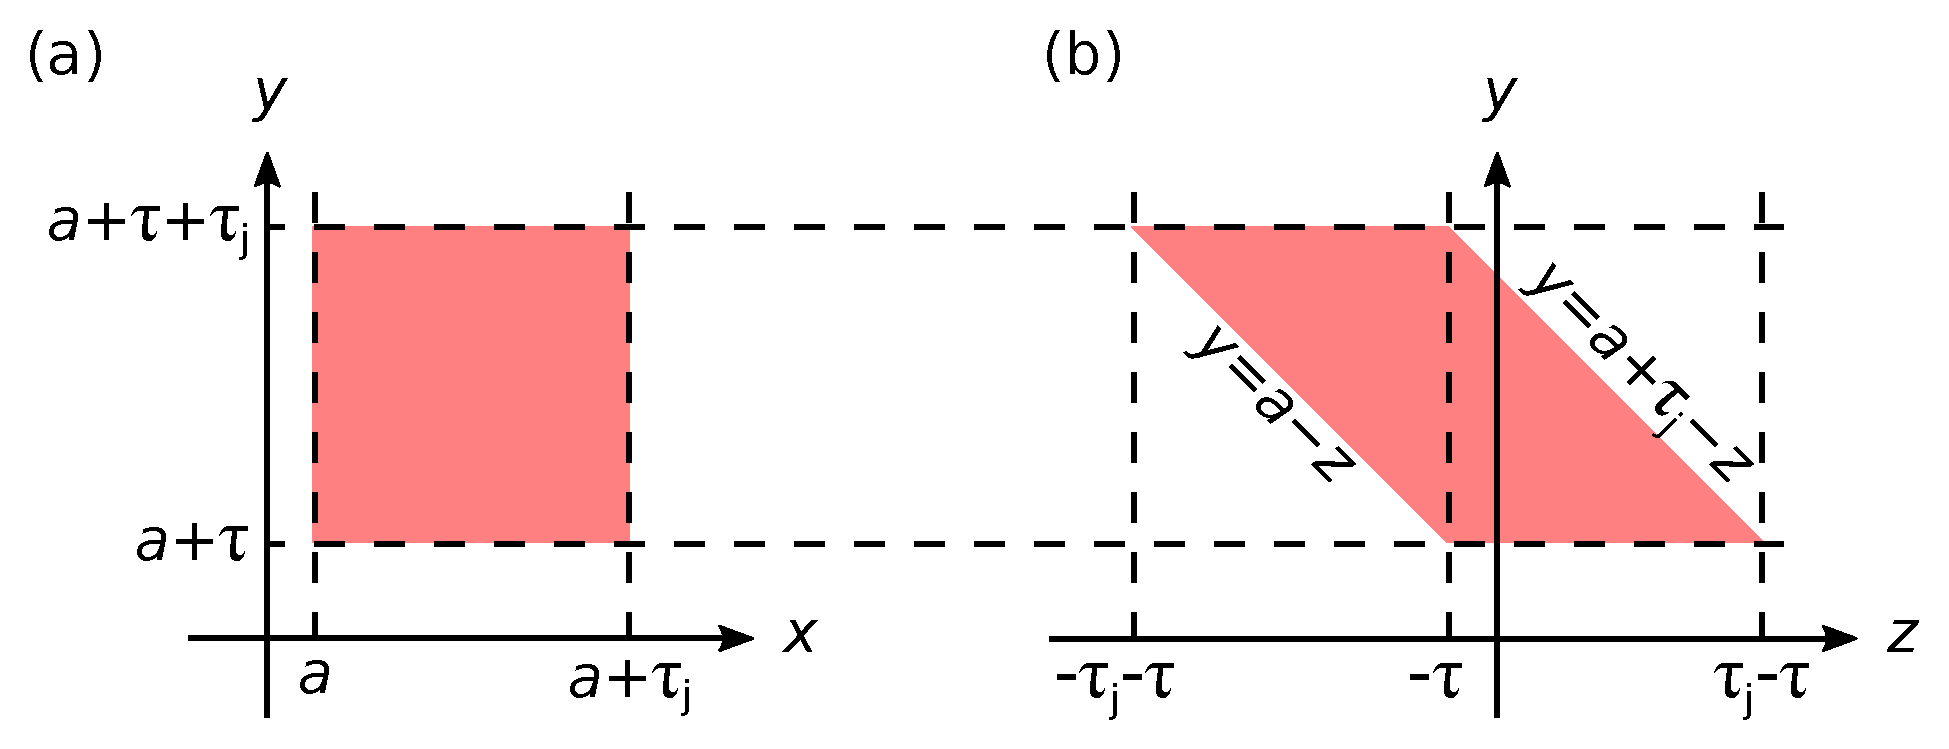
\includegraphics[width = \textwidth]{%
    Appendices/OscillatorPhaseNoise/figs/integration_domains.pdf}
  \caption[Integration domains]{
    Integration domains (a) before and (b) after
    the change of variables in
    (\ref{eq:OscillatorPhaseNoise:change_of_variables}).}
  \label{fig:OscillatorPhaseNoise:integration_domains}
\end{figure}
%
\chapter{Sound-wave characterization}
\label{app:SoundWaveCharacterization}
\begin{itemize}
  \item Sound-wave dispersion relation
\end{itemize}


\section{Hardware}
\label{sec:SoundWaveCharacterization:Hardware}
\subsection{Speaker}
\label{sec:SoundWaveCharacterization:Hardware:speaker}
\subsection{Calibrated microphone}
\label{sec:SoundWaveCharacterization:Hardware:microphone}
\subsection{Test stand}
\label{sec:SoundWaveCharacterization:Hardware:test_stand}


\section{Sound-wave measurements}
\label{sec:SoundWaveCharacterization:Measurements}
To lowest order, the speaker is cylindrically symmetric.
Thus, the sound waves are expected to have
axial, radial, and frequency dependencies.
Sections~\ref{sec:SoundWaveCharacterization:Measurements:amlitude} through
\ref{sec:SoundWaveCharacterization:Measurements:phasing}
summarize these measurements and their implications
for the sound-wave model developed in
Section~\ref{sec:SoundWaveCharacterization:Model}.


\subsection{On-axis amplitude}
\label{sec:SoundWaveCharacterization:Measurements:amlitude}
After centering the microphone on the speaker's symmetry axis,
the on-axis amplitude can be easily characterized by
varying both the frequency $f$ of the sound waves and
the microphone height $z$ above the speaker face.
The frequencies $f$ and heights $z$
are motivated by the parameters of the heterodyne interferometer
described in Chapter~\ref{ch:Implementation}.
Specifically, the interferometer spatial bandwidth
$|k| \leq \SI{5}{\per\centi\meter}$
from (\ref{eq:Implementation:kfsv_interferometer_design}) motivates
sound-wave measurements at frequencies
$f \lesssim \SI{30}{\kilo\hertz}$
(i.e.\ $|k| \lesssim \SI{5}{\per\centi\meter}$).
Further, to produce a robust interference signal
during sound-wave calibrations,
the speaker is placed very close
to the edge of the collimated probe beam,
which has 1/e $E$ radius $w_0 = \SI{3.4}{\centi\meter}$;
thus, sound-wave measurements are made at heights
spanning the probe-beam profile
$z
=
\{\SI{2.5}{\centi\meter}, \SI{5.5}{\centi\meter}, \SI{8.5}{\centi\meter}\}$.
The on-axis amplitude of the sound waves as a function of
wavenumber $k$ and height $z$ above the speaker face is shown in
Fig.~\ref{fig:SoundWaveCharacterization:tymphany_on_axis_amplitude}.
As expected, the on-axis amplitude decreases with
increasing distance $z$ from the speaker face.
Further, the on-axis amplitude has a complicated wavenumber dependence, but
it is relatively flat for
$\SI{1}{\per\centi\meter} \lesssim k \lesssim \SI{3.5}{\per\centi\meter}$.

\begin{figure}
  \centering
  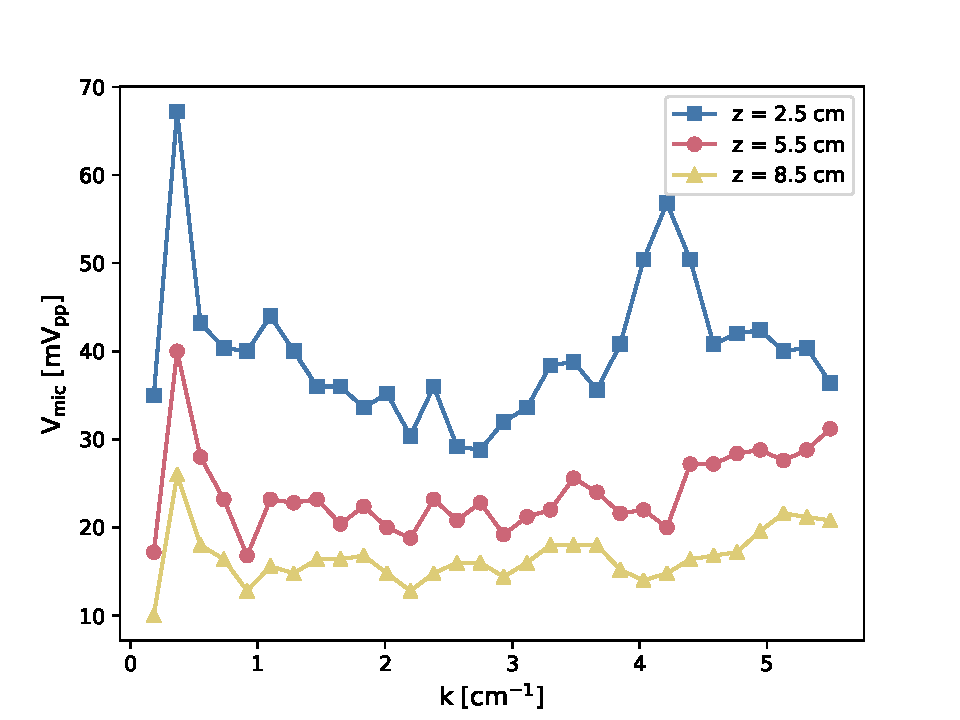
\includegraphics[width = \textwidth]{%
    Appendices/SoundWaveCharacterization/figs/tymphany_on_axis_amplitude.pdf}
  \caption[On-axis amplitude of sound waves]{%
    On-axis amplitude of sound waves as a function of
    wavenumber $k$ and height $z$ above the speaker face.
    Note that the amplitude is specified
    as a \emph{peak-to-peak} value.
  }
\label{fig:SoundWaveCharacterization:tymphany_on_axis_amplitude}
\end{figure}


\subsection{Wavefront phasing}
\label{sec:SoundWaveCharacterization:Measurements:phasing}
Characterizing the sound-wave phasing is somewhat more involved
than characterizing the on-axis amplitude,
as it requires measurements at several radial positions $\rho$
for each frequency $f$ and microphone height $z$.
For this reason, the wavefront-phasing measurements
are more coarsely sampled in frequency $f$
than the on-axis amplitude measurements in
Section~\ref{sec:SoundWaveCharacterization:Measurements:amlitude}.
For a given frequency $f$ and height $z$,
the sound-wave phasing is measured by
tracking a point of constant phase in the microphone waveform
as the radial position $\rho$ is varied;
such tracking can be easily accomplished
by triggering the oscilloscope
with a copy of the waveform that is driving the speaker.
To begin the radial scan,
the microphone height $z$ is selected, and
the microphone is displaced from the speaker's symmetry axis
by a few centimeters.
Then, in $\SI{1}{\centi\meter}$ increments,
the microphone is moved radially inwards towards the center;
upon passing through the center,
the radial scan is continued in $\SI{1}{\centi\meter}$ increments
until the sound-wave amplitude becomes negligible.
Note that beginning the radial scan
with a small displacement from the symmetry axis
allows empirical identification of the symmetry-axis location
(by e.g.\ fitting the measured amplitude and/or phasing
and identifying the extremum that occurs at the symmetry axis).

\begin{figure}
  \centering
  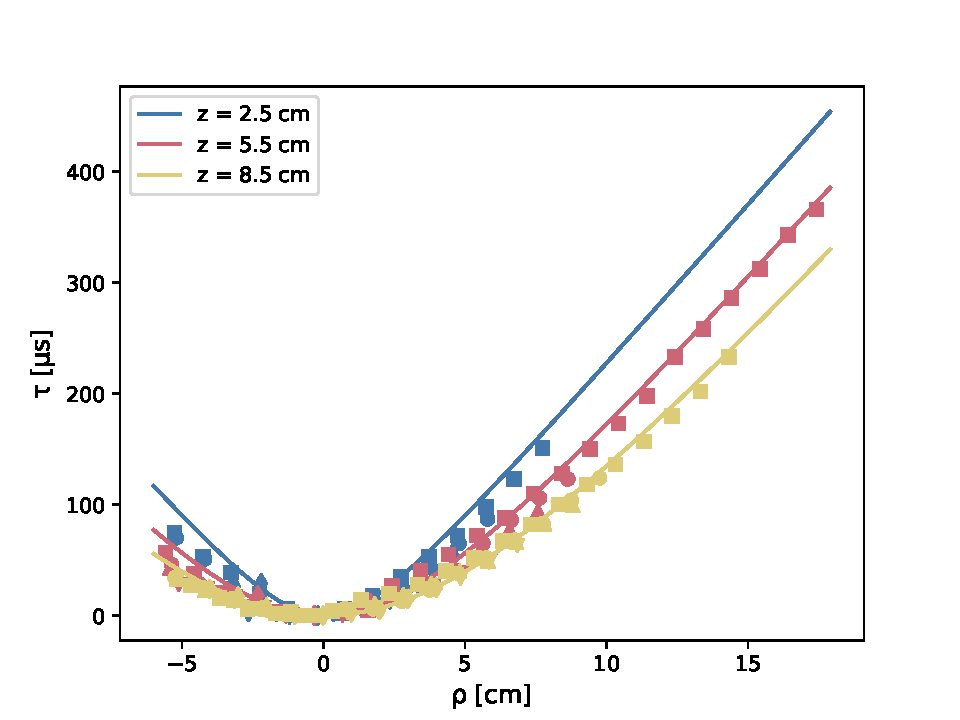
\includegraphics[width = \textwidth]{%
    Appendices/SoundWaveCharacterization/figs/tymphany_wavefront_phasing.pdf}
  \caption[Wavefront phasing of sound waves]{%
    Wavefront phasing of sound waves.
    The symbols show the measured time delay $\tau$
    between the wavefront at height $z$ and radial displacement $\rho$ and
    the corresponding on-axis wavefront (i.e.\ same $z$ but $\rho = 0$),
    with each symbol shape corresponding to particular frequency.
    The traces correspond to the time delay
    (\ref{eq:SoundWaveCharacterization:time_delay})
    predicted for spherical waves.
    The close proximity of the measured points to the spherical-wave traces
    indicates that, to lowest order, the waves are approximately spherical
    over the spatial domain and frequencies probed.
  }
\label{fig:SoundWaveCharacterization:tymphany_wavefront_phasing}
\end{figure}

At sufficiently large distances,
the speaker will behave like a point source,
producing sound waves with spherical wavefronts.
This point-source approximation is taken as a reasonable
starting point for the investigation of the wavefront phasing.
If a sound wave is measured on axis at height $z$ above the speaker,
the corresponding wavefront will subsequently arrive
at position $r = (z^2 + \rho^2)$
delayed by a time $\tau$
\begin{equation}
  \tau = \frac{r - z}{c_s},
  \label{eq:SoundWaveCharacterization:time_delay}
\end{equation}
\graffito{\textcolor{red}{value for $c_s$}}
where $c_s$ is the sound speed.
Fig.~\ref{fig:SoundWaveCharacterization:tymphany_wavefront_phasing}
compares the measured time delay to
the time delay predicted for spherical waves
(\ref{eq:SoundWaveCharacterization:time_delay})
as a function of height $z$, radial position $\rho$, and frequency $f$.
Clearly, to lowest order, the waves are approximately spherical
over the spatial domain and frequencies probed.


\subsection{Spatial envelope}
\label{sec:SoundWaveCharacterization:Measurements:envelope}
If the sound-wave amplitude is also measured
during the radial scans described in
Section~\ref{sec:SoundWaveCharacterization:Measurements:phasing},
the spatial envelope of the sound waves can also be quantified.
Fig.~\ref{fig:SoundWaveCharacterization:tymphany_spatial_envelope_z_5_5cm}
displays the spatial envelopes of sound waves of various frequencies $f$
at height $z = \SI{5.5}{\centi\meter}$ above the face of the speaker.
Clearly, the width of the spatial envelope decreases
with increasing frequency $f$.
Measurements at other heights $z$
exhibit qualitatively similar behavior.

\begin{figure}
  \centering
  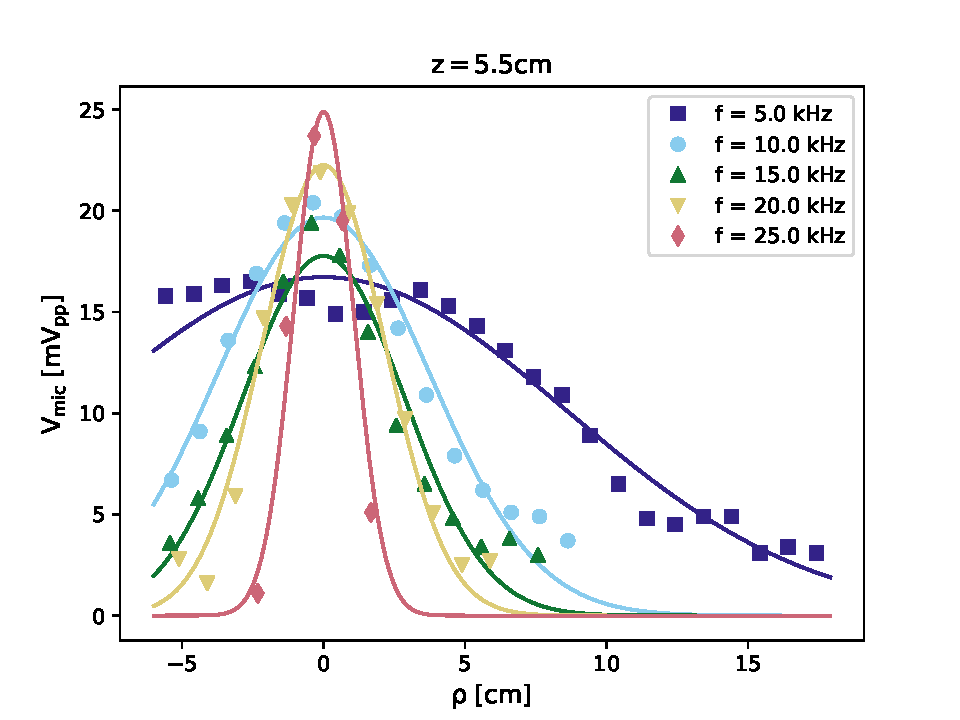
\includegraphics[width = \textwidth]{%
    Appendices/SoundWaveCharacterization/figs/tymphany_spatial_envelope_z_5_5cm.pdf}
  \caption[Representative spatial envelopes of sound waves]{%
    Sound-wave spatial envelopes for frequencies $f$
    at height $z = \SI{5.5}{\centi\meter}$ above the face of the speaker.
    Symbols indicate measurement points, while
    the traces correspond to Gaussian fits of the form
    (\ref{eq:SoundWaveCharacterization:Gaussian}).
    Measurements and fits at other heights $z$
    exhibit qualitatively similar trends.
  }
\label{fig:SoundWaveCharacterization:tymphany_spatial_envelope_z_5_5cm}
\end{figure}

The narrowing of the spatial envelope with increasing frequency
can be quantified by fitting the measurements
to an assumed functional form.
To lowest order, the spatial envelopes are well approximated by a Gaussian
\begin{equation}
  V_{\text{mic}}(\rho)
  =
  V_0(z, f)
  \exp\left[
    \frac{-\rho^2}{w(z, f)^2}
  \right],
  \label{eq:SoundWaveCharacterization:Gaussian}
\end{equation}
where $w(z, f)$ is the 1/e radius, which
is a function of the height $z$ and the sound-wave frequency $f$.
Gaussian fits to the envelope measurements are also shown in
Fig.~\ref{fig:SoundWaveCharacterization:tymphany_spatial_envelope_z_5_5cm}.
Deviations from a Gaussian are most apparent at low frequencies;
this may be attributable to baffle diffraction across the speaker face but
was not further investigated.
The approximation of a Gaussian envelope
will be sufficiently accurate for the present work.
Fig~\ref{fig:SoundWaveCharacterization:tymphany_gaussian_widths}
displays the fitted 1/e Gaussian radii $w$ as a function of
sound-wave wavenumber $k$ and
height $z$ above the face of the speaker.
As previously and anecdotally noted for $z = \SI{5.5}{\centi\meter}$,
the width of the spatial envelope $w$
decreases with increasing $k$ for each height $z$.
Further, $w$ increases with increasing $z$, which
results from free-space diffraction of the sound wave.

\begin{figure}
  \centering
  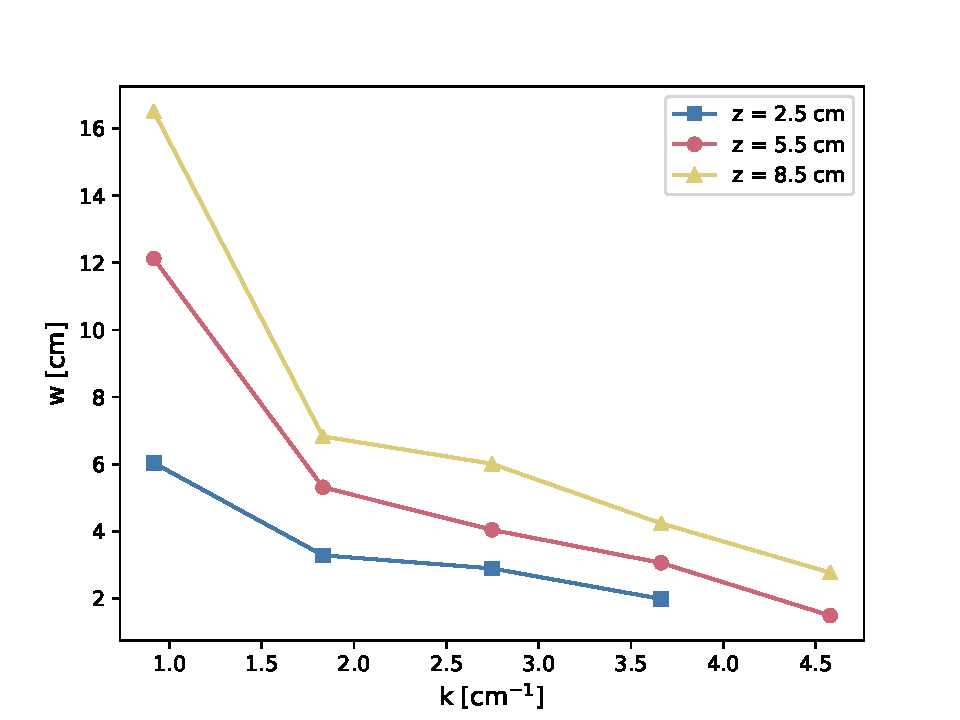
\includegraphics[width = \textwidth]{%
    Appendices/SoundWaveCharacterization/figs/tymphany_gaussian_widths.pdf}
  \caption[Gaussian widths of sound waves]{%
    Fitted 1/e Gaussian radii $w$ of sound waves
    as a function of sound-wave wavenumber $k$ and
    height $z$ above the face of the speaker.
  }
\label{fig:SoundWaveCharacterization:tymphany_gaussian_widths}
\end{figure}


\section{Sound-wave model}
\label{sec:SoundWaveCharacterization:Model}


\section{Perturbed index of refraction}
\label{sec:SoundWaveCharacterization:PerturbedIndexOfRefractiion}


\bibliographystyle{plainurl}
\bibliography{references}
%
\chapter{Spectral estimation}
\label{app:SpectralEstimation}
In contrast to deterministic processes,
random processes cannot be modeled via an explicit mathematical relationship.
Rather, random processes are characterized
in terms of probabilities and statistical properties.
Any given observation of a random process represents
only one of many possible observations;
each such observation is referred to as
a ``sample'' or a ``realization'' of the random process
and is denoted as $x_k(t)$.
The random process itself consists of
the ensemble of all of the potential observations
and is denoted as $\{x_k(t)\}$.
Random processes can be stationary or nonstationary.
The statistical properties of a stationary random process
do not vary in time, and
the spectral tools discussed below
are all developed for analysis of stationary random processes.


\section{Non-parametric techniques}
\label{app:SpectralEstimation:NonParametric}
Most of the discussion below is distilled from
the seminal work by Bendat and Piersol~\cite{bendat_and_piersol}, and
inquisitive readers are directed there
for a more extensive treatment of the subject.

The windowed, finite Fourier transform $X_k(f, T)$
of a continuous signal $x_k(t)$
sampled for $-T / 2 \leq t < T / 2$
is defined as
\begin{equation}
  X_k(f, T)
  =
  \int_{-T / 2}^{T / 2}
  dt \, [w(t) \cdot x_k(t)] e^{-i \, 2 \pi f t},
  \label{eq:SpectralEstimation:finite_Fourier_transform}
\end{equation}
where $w(t)$ is an arbitrary windowing function.
Typically, the selected windowing function smoothly tapers
as $|t| \rightarrow T / 2$
to minimize side-lobe ``leakage''
that results from discontinuities at the start and end of the sample record.
Further, to prevent power loss, the windowing function
is also typically normalized such that
\begin{equation}
  \frac{1}{T} \int_{-T/2}^{T/2} dt \, [w(t)]^2 = 1.
\end{equation}
The normalized Hanning window is perhaps
the most commonly used windowing function, and
it is used uniformly throughout this work.

For real-valued, stationary random processes $\{x_k(t)\}$ and $\{y_k(t)\}$,
the one-sided \emph{cross-spectral density} function $G_{xy}(f)$ is defined as
\begin{equation}
  G_{xy}(f)
  \equiv
  \lim_{T \rightarrow \infty}
  \frac{2}{T} E \left[ X_k^*(f, T) Y_k(f, T) \right]
  \label{eq:SpectralEstimation:cross_spectral_density_defn}
\end{equation}
for $0 < f < \infty$;
$G_{xy}(f)$ is not defined for $f < 0$, and
it is reduced by a factor of two relative to
(\ref{eq:SpectralEstimation:cross_spectral_density_defn}) at $f = 0$
(the value of $G_{xy}(0)$ is of little relevance to this work).
Note that $E[\cdot]$ is the expectation value operator;
this operator averages over all of the realizations in the ensemble, and
its application ensures that
(\ref{eq:SpectralEstimation:cross_spectral_density_defn})
is a statistically consistent definition of the cross-spectral density
(that is, ensemble averaging is needed for $G_{xy}(f)$
to approach the true cross-spectral density
as $T \rightarrow \infty$). % see pgs. 127, 128 of Bendat & Piersol, 4th ed.
If, in addition to being stationary,
the random process is also \emph{ergodic},
the ensemble average can be replaced
with a time average of $X_k(f, T)$
over successive time slices.
If desired, these time slices may partially overlap.
Unless otherwise noted,
all of the ensemble averages in this work are computed
using this assumption of ergodicity, and
successive slices are selected to overlap by 50\%.

In general $G_{xy}(f)$ is a complex-valued function.
This can be made explicit by writing
\begin{equation}
  G_{xy}(f) = \left| G_{xy}(f) \right| e^{i \alpha_{xy}(f)},
  \label{eq:SpectralEstimation:cross_spectral_density_explicit_complex}
\end{equation}
where $\alpha_{xy}(f)$ is the \emph{phase angle}.
Note that if
$\lim_{T \rightarrow \infty} E[X_k(f, T)] \propto e^{i \alpha_x}$ and
$\lim_{T \rightarrow \infty} E[Y_k(f, T)] \propto e^{i \alpha_y}$, then
\begin{equation}
  \alpha_{xy} = \alpha_y - \alpha_x.
\end{equation}
Further, note that for the special case $\{x_k(t)\} = \{y_k(t)\}$,
$G_{xx}(f)$ is real-valued (i.e.\ $G_{xx}(f) = |G_{xx}(f)|$) and
is referred to as the one-sided \emph{autospectral density} function.

The degree of correlation between random processes
$\{x_k(t)\}$ and $\{y_k(t)\}$ can be easily quantified
with the corresponding spectral density functions.
In particular, the \emph{magnitude-squared coherence} function
$\gamma_{xy}^2(f)$ is defined as
\begin{equation}
  \gamma_{xy}^2(f)
  \equiv
  \frac{|G_{xy}(f)|^2}{G_{xx}(f) G_{yy}(f)},
  \label{eq:SpectralEstimation:magnitude_squared_coherence_defn}
\end{equation}
and it satisfies
\begin{equation}
  0 \leq \gamma_{xy}^2(f) \leq 1
  \label{eq:SpectralEstimation:magnitude_squared_coherence_bounds}
\end{equation}
for $0 \leq f < \infty$.
If $\gamma_{xy}^2(f) = 1$,
$\{x_k(t)\}$ and $\{y_k(t)\}$ are $100\%$ correlated at frequency $f$, and
if $\gamma_{xy}^2(f) = 0$,
$\{x_k(t)\}$ and $\{y_k(t)\}$ are completely uncorrelated at frequency $f$.
Note that the ensemble-averaging operation in
(\ref{eq:SpectralEstimation:cross_spectral_density_defn})
is paramount to the computation
of \emph{informative} values for $\gamma_{xy}^2(f)$;
that is, if ensemble averaging is ignored, and
only single realizations of the random processes are used,
$\gamma_{xy}^2(f) \equiv 1$ for all $f$,
\emph{regardless} of the actual degree of coherence
between between $\{x_k(t)\}$ and $\{y_k(t)\}$.

Care should be taken when computing spectral density estimates.
Table~\ref{table:ToroidalCorrelation:spectral_estimate_random_errors}
summarizes the random errors associated with the estimates
of various spectral properties.
Note that the number of realizations $N_r$ used
in the computation of the ensemble average
is a parameter that can be specified
at the time of analysis and that
increasing $N_r$ reduces the random errors of each spectral estimate.
(While increased $\gamma_{xy}^2(f)$ also reduces random errors,
$\gamma_{xy}^2(f)$ is an intrinsic property of the data
rather than a parameter that can be specified at the time of analysis).
Further, in various programming languages,
it is not uncommon to ``detrend'' realizations $x_k(t)$ and $y_k(t)$
by subtracting the signal mean or linear trend
prior to application of
(\ref{eq:SpectralEstimation:cross_spectral_density_defn}).
However, the author anecdotally notes that his experience with
such detrending can lead to values of $\gamma_{xy}^2(f)$
that unphysically exceed the bounds established in
(\ref{eq:SpectralEstimation:magnitude_squared_coherence_bounds}).
The subtleties of such discrepancies were not investigated further, and
no such detrending was applied to signals
prior to spectral computations in this work;
instead, if needed, signals are high-pass filtered as described in
Section~\ref{sec:Implementation:DataPreparation:high_pass_filtering}.

\begin{table}[t]
  \centering
  \renewcommand{\arraystretch}{1.5}% Spread rows out...
  \begin{tabular}{%
    >{\centering}m{5.0cm} >{\centering}m{5.0cm}
  }
    \toprule%
    \textbf{Spectral estimate}
    & \textbf{Random error} \cite{bendat_and_piersol}
    \tabularnewline%
    \midrule
    $G_{xy}(f)$
    & $\varepsilon \left[G_{xy}(f) \right]
    =
    \frac{1}{|\gamma_{xy}(f)| \sqrt{N_r}}$
    \tabularnewline%
    $\alpha_{xy}(f)$
    & s.d.$\left[ \alpha_{xy}(f) \right]
    \approx
    \frac{[1 - \gamma_{xy}^2(f)]^{1/2}}{|\gamma_{xy}(f)| \sqrt{2 N_r}}$
    \tabularnewline%
    $\gamma_{xy}^2(f)$
    & $\varepsilon \left[ \gamma_{xy}^2(f) \right]
    =
    \frac{\sqrt{2} [1 - \gamma_{xy}^2(f)]}{|\gamma_{xy}(f)| \sqrt{N_r}}$
    \tabularnewline%
    \toprule%
  \end{tabular}
  \caption[Random errors in spectral estimates]{%
    Random errors in estimates of spectral properties are functions of
    the number of realizations $N_r$ used
    in the computation of the ensemble average and
    the coherence magnitude $|\gamma_{xy}(f)|$.
    Here, s.d$[\cdot]$ represents the standard deviation of the estimate, and
    $\varepsilon[\cdot]$ represents the standard deviation of the estimate
    \emph{normalized} to the true value of the spectral property.
    }%
\label{table:ToroidalCorrelation:spectral_estimate_random_errors}
\end{table}


\section{Parametric techniques}
\label{app:SpectralEstimation:Parametric}


\bibliographystyle{plainurl}
\bibliography{references}
%
\chapter{Synchronization of digital records}
\label{app:DigitizerSynchronization}
Digital signal processing is often foundational to signal analysis.
Of course, application of such techniques
requires converting an analog signal to a digital record.
Efficient conversion requires
both quantization of the signal magnitude and
temporal sampling~\cite{bennett_bstj48}.
When examining the phasing between multiple digital records,
the synchronization of this temporal sampling
is of paramount importance.

This appendix discusses post-processing synchronization of digital records.
Below, Section~\ref{app:DigitizerSynchronization:temporal_sampling}
defines temporal sampling and
mentions caveats regarding nominal and actual sampling parameters.
Section~\ref{app:DigitizerSynchronization:digitization_schemes}
then discusses various digitization schemes,
highlighting which schemes allow synchronization.
Finally, Section~\ref{app:DigitizerSynchronization:phase_locked_synchronization}
details the synchronization of phase-locked digital records.


\section{Temporal sampling}
\label{app:DigitizerSynchronization:temporal_sampling}
Typically, temporal sampling of signal $x_j(t)$ occurs
at a fixed sampling rate $F_j$ such that
successive points in the digital record
are separated in time by $1 / F_j$.
Digitization begins at the trigger time $t_j[0]$ such that
the $m\ts{th}$ digitized point is sampled at time
\begin{equation}
  t_j[m] = t_j[0] + \frac{m}{F_j}.
  \label{eq:DigitizerSynchronization:timebase_generic}
\end{equation}
Ideally, the \emph{realized} sampling rate $F_j$ and trigger time $t_j[0]$
are equal to their \emph{nominal} values
$F_j^{\nom}$ and $t_j^{\nom}[0]$, respectively.
However, short-term jitter, long-term drifts, and constant offsets
often plague real-world digitization such that
$F_j \neq F_j^{\nom}$, $t_j[0] \neq t_j^{\nom}[0]$, and
\begin{equation}
  t_j[m] \neq t_j^{\nom}[0] + \frac{m}{F_j^{\nom}};
\end{equation}
that is, the actual sample times of the digital record
differ from their nominal values.
In a properly operating digitizer,
these discrepancies are typically small, and
an autospectral-density estimate (for example)
of $x_j(t)$ from its digital record
will be negligibly compromised.
When estimating the \emph{phasing}
between $x_j(t)$ and $x_{k}(t)$ for $j \neq k$, however,
identifying and correcting such timebase discrepancies
becomes paramount in importance.


\section{Which digital records can be synchronized?}
\label{app:DigitizerSynchronization:digitization_schemes}
The digitization scheme determines
whether or not digital records
$\{x_j[m]\}$ and $\{x_k[m]\}$
can be synchronized.
The cleanest, simplest, and most problem-free scheme
is to digitize $x_j(t)$ and $x_k(t)$ on the \emph{same} system
such that the actual sample rates and trigger times
of both digital records are identical
(i.e.\ $F_j = F_k$ and $t_j[0] = t_k[0]$, respectively).
However, such a scheme is not always feasible.
Further, note that multiple digitizer boards
operating in a master-slave configuration
can still suffer from trigger-time offsets,
despite nominally being part of the same digitization system.
The next-best scheme is to use phase-locked digitizers
such that
\begin{equation}
  \frac{F_j}{F_k}
  =
  \frac{F_j^{\nom}}{F_k^{\nom}}
  =
  \text{constant (for \emph{phase-locked} digitizers)},
  \label{eq:DigitizerSynchronization:phase_locked_constraint}
\end{equation}
regardless of any short-term jitter or long-term drift
in the digitizer clocks.
As shown in
Section~\ref{app:DigitizerSynchronization:phase_locked_synchronization},
the actual sampling times of phase-locked digital records
differ (at most) by a constant ``trigger offset'',
which can be compensated easily.
Finally, the least-desirable scheme
is to use free-running digitizers
such that $F_j / F_k \neq F_j^{\nom} / F_k^{\nom}$;
it may be impossible to synchronize records
from free-running digitizers.
While the below discussion considers
synchronization via post-processing,
it should be noted for completeness
that hardware solutions for synchronization also exist
\cite{stillerman_fed10}.


\section{Synchronization of phase-locked digital records}
\label{app:DigitizerSynchronization:phase_locked_synchronization}
This section details the synchronization of phase-locked digital records.
Specifically, Section~\ref{app:DigitizerSynchronization:phase_locked_synchronization:trigger_offset}
defines the ``trigger offset'' between phase-locked digital records, and
Section~\ref{app:DigitizerSynchronization:phase_locked_synchronization:trigger_offset_effect}
discusses the phase bias produced by a finite trigger offset.
Section~\ref{app:DigitizerSynchronization:phase_locked_synchronization:trigger_offset_estimates}
describes methods for estimating the trigger offset.
Then, using standard techniques~\cite[Sec.~4.5]{oppenheim},
the trigger offset can be compensated easily in post-processing,
even if the offset is a non-integer multiple of the sample spacing.


\subsection{The ``trigger offset''}
\label{app:DigitizerSynchronization:phase_locked_synchronization:trigger_offset}
Phase-locked digitizers may suffer from a deleterious ``trigger offset''.
To see this, consider two digitizers $j$ and $k$.
Assume that the digitizers have different nominal trigger times
$t_j^{\nom}[0] \neq t_k^{\nom}[0]$ but
the same nominal sampling rate
$F_j^{\nom} = F_k^{\nom}$.
(If the digitizers have different nominal sampling rates, however,
the records from one of the digitizers
can be digitally resampled~\cite[Sec.~4.6]{oppenheim}
with the sampling rate of the other digitizer, and
then the presentation below proceeds unchanged).
Because the nominal trigger times of digitizers $j$ and $k$ differ,
their $m\ts{th}$ nominal timestamps also differ,
i.e.\ $t_j^{\nom}[m] \neq t_k^{\nom}[m]$.
Instead, $t_j^{\nom}[m] = t_k^{\nom}[n]$, where
\begin{equation}
  n
  =
  m
  +
  F_j^{\nom}
  \left(
    t_j^{\nom}[0]
    -
    t_k^{\nom}[0]
  \right),
  \label{eq:DigitizerSynchronization:nominal_timebase_index_relation}
\end{equation}
and the equality of the nominal sampling rates has been utilized.
Now, for digitizer $j$ define
$\delta t_j = t_j[0] - t_j^{\nom}[0]$
to be the difference between the actual and nominal trigger times,
$\delta F_j = F_j - F_j^{\nom}$
to be the difference between the actual and nominal sampling rates, and
$\bar{\delta F_j} = \delta F_j / F_j^{\nom}$
to be the normalized difference between the actual and nominal sampling rates
($|\bar{\delta F_j}| \ll 1$).
Similar definitions apply for digitizer $k$.
Because the digitizers satisfy the phase-locked constraint
(\ref{eq:DigitizerSynchronization:phase_locked_constraint}),
\begin{equation}
  \bar{\delta F_j} = \bar{\delta F_k}.
  \label{eq:DigitizerSynchronization:phase_locked_normalized_sample_rate_deviations}
\end{equation}
(Note that equality
(\ref{eq:DigitizerSynchronization:phase_locked_normalized_sample_rate_deviations})
holds even if the nominal sampling rates are different).
Then, to first order in $\bar{\delta F_j}$,
the actual sampling times $t_j[m]$
are related to the nominal sampling times $t_j^{\nom}[m]$ via
\begin{equation}
  t_j[m]
  \approx
  t_j^{\nom}[m]
  +
  \delta t_j
  -
  \frac{m \cdot \bar{\delta F_j}}{F_j^{\nom}}.
  \label{eq:DigitizerSynchronization:timebase_actual_vs_nominal}
\end{equation}
Thus, trigger-time discrepancy $\delta t_j$
produces a constant offset
between the actual and nominal sampling times of digitizer $j$, while
sampling-rate discrepancy $\delta F_j$
produces a linear ramp
between the actual and nominal sampling times of digitizer $j$.

Now, in some situations it is of the utmost importance
that the actual sampling times of digitizers $j$ and $k$ align.
(Inferring the spatial structure of a signal from its phasing
between two spatially separated sensors is one such example).
The \emph{nominal} sampling times are aligned via
(\ref{eq:DigitizerSynchronization:nominal_timebase_index_relation}), but
any remaining discrepancy between the \emph{actual} sampling times is
\begin{align}
  \delta t_{\trig}
  &=
  t_j[m] - t_k[n]
  \notag \\
  &=
  \left( \delta t_j - \delta t_k \right)
  +
  \bar{\delta F_j} \left( t_j^{\nom}[0] - t_k^{\nom}[0] \right);
  \label{eq:DigitizerSynchronization:trigger_offset}
\end{align}
this situation is shown schematically in
Figure~\ref{fig:DigitizerSynchronization:trigger_offset_schematic}.
Here, the first term on the right-hand side of
(\ref{eq:DigitizerSynchronization:trigger_offset})
corresponds to the difference between
trigger-time discrepancies of each digitizer, while
the second term on the right-hand side
corresponds to the relative sampling-rate discrepancy
weighted by the difference in nominal trigger times.
As both effects are related to triggering,
this timestamp discrepancy is referred to as
the ``trigger offset'' $\delta t_{\trig}$.
Note that $\delta t_{\trig}$ is a single, constant value
for any given pair of phase-locked digital records.

\begin{figure}
  \centering
  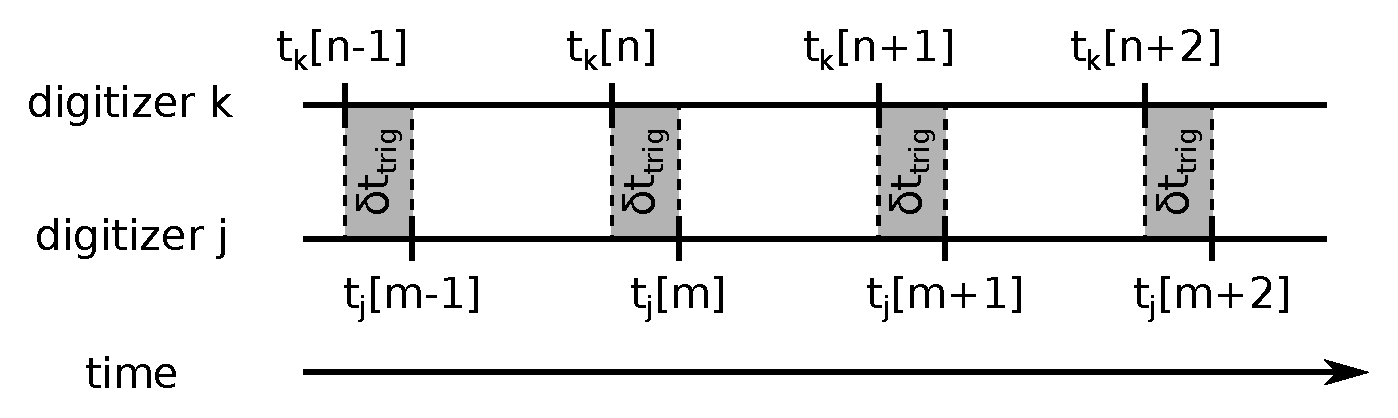
\includegraphics[width = \textwidth]{%
    Appendices/DigitizerSynchronization/figs/trigger_offset_schematic.pdf}
  \caption[``Trigger offset'' between phase-locked digitizers]{%
    The ``trigger offset'' $\delta t_{\trig}$ between phase-locked digitizers.
    Here, the $n\ts{th}$ nominal sampling time of digitizer $k$ equals
    the $m\ts{th}$ nominal sampling time of digitizer $k$
    (i.e.\ $t_j^{\nom}[m] = t_k^{\nom}[n]$), where
    $n$ and $m$ are related via
    (\ref{eq:DigitizerSynchronization:nominal_timebase_index_relation}).
    However, a finite trigger offset
    (\ref{eq:DigitizerSynchronization:trigger_offset})
    produces a discrepancy between the \emph{actual} sampling times
    of the two digitizers (i.e.\ $t_j[m] \neq t_k[n]$),
    which can bias phase measurements, as discussed in
    Section~\ref{app:DigitizerSynchronization:phase_locked_synchronization:trigger_offset_effect}.
  }
\label{fig:DigitizerSynchronization:trigger_offset_schematic}
\end{figure}


\subsection{Effect of the trigger offset}
\label{app:DigitizerSynchronization:phase_locked_synchronization:trigger_offset_effect}
The trigger offset (\ref{eq:DigitizerSynchronization:trigger_offset})
biases the measured phasing between the digital records.
To see this, let $x_j(t)$ be a coherent mode
of angular frequency $\omega$ such that
the corresponding digital record is
\begin{align}
  x_j[m]
  &=
  x_j(t_j[m])
  \notag \\
  &\propto
  X_j(\omega) e^{i \omega t_j[m]}
  \notag \\
  &=
  |X_j(\omega)| e^{i \{ \alpha_j(\omega) + \omega t_j[m]\}},
\end{align}
where $|X_j(\omega)|$ is the Fourier amplitude and
$\alpha_j(\omega)$ is the Fourier phase.
(Here, the Fourier-transform kernel is $\propto e^{-i \omega t}$ and
the inverse Fourier-transform kernel is $\propto e^{i \omega t}$,
in accord with the NumPy implementation
of the fast Fourier transform (FFT)~\cite{numpy_fft};
if the opposite convention is used for FFT computations,
then the substitution $\delta t_{\trig} \rightarrow -\delta t_{\trig}$
should be made in equations
(\ref{eq:DigitizerSynchronization:measured_phase_difference}),
(\ref{eq:DigitizerSynchronization:trigger_offset_estimate_apriori_phase}), and
(\ref{eq:DigitizerSynchronization:trigger_offset_estimate_frequency_swept})).
Then, after aligning \emph{nominal} sampling times via
(\ref{eq:DigitizerSynchronization:nominal_timebase_index_relation}),
the \emph{measured} phase difference $\Delta \alpha_{\meas}$
between digital records $\{x_j[m]\}$ and $\{x_k[n]\}$ is
\begin{align}
  \Delta \alpha_{\meas}
  &=
  \arg\left(
    x_k^*[n]
    \cdot
    x_j[m]
  \right)
  \notag \\
  &=
  \left[
    \alpha_j(\omega)
    -
    \alpha_k(\omega)
  \right]
  +
  \omega
  \left(
    t_j[m] - t_k[n]
  \right)
  \notag \\
  &=
  \Delta \alpha(\omega)
  +
  \left( \omega \cdot \delta t_{\trig} \right),
  \label{eq:DigitizerSynchronization:measured_phase_difference}
\end{align}
where $\Delta \alpha(\omega) = \alpha_j(\omega) - \alpha_k(\omega)$
is the true phase difference and
$\delta t_{\trig}$ is defined in
(\ref{eq:DigitizerSynchronization:trigger_offset}).
Thus, non-zero trigger offset $\delta t_{\trig}$ biases
the measured phase difference $\Delta \alpha_{\meas}$
away from the true phase difference $\Delta \alpha$.
The above argument readily extends to broadband signals.


\subsection{Estimating the trigger offset}
\label{app:DigitizerSynchronization:phase_locked_synchronization:trigger_offset_estimates}
Clearly, a finite trigger offset is undesirable.
In some situations, it is possible
to estimate the trigger offset.
Then, using standard techniques~\cite[Sec.~4.5]{oppenheim},
the trigger offset can be compensated easily in post-processing,
even if the offset is a non-integer multiple of the sample spacing.

If the true phase difference $\Delta \alpha(\omega)$
is known \emph{a priori} (from e.g.\ another measurement),
solving for $\delta t_{\trig}$ in
(\ref{eq:DigitizerSynchronization:measured_phase_difference})
yields an estimated trigger offset
\begin{equation}
  \delta t_{\trig}
  =
  \frac{\Delta \alpha_{\meas}(\omega) - \Delta \alpha(\omega)}{\omega}.
  \label{eq:DigitizerSynchronization:trigger_offset_estimate_apriori_phase}
\end{equation}
Although \emph{a priori} knowledge of $\Delta \alpha$ may make
(\ref{eq:DigitizerSynchronization:trigger_offset_estimate_apriori_phase})
seem rather academic,
it does find real-world application.
For example, imagine the signals from
a regularly spaced array of channels
are digitized across multiple digitizer boards.
The intra-board trigger offsets are negligible
such that the true phase difference $\Delta \alpha$
can be accurately estimated from
adjacent channels digitized on the same board;
comparing this estimate of $\Delta \alpha$
to the measured phase difference $\Delta \alpha_{\meas}$
between adjacent channels digitized on different boards
via (\ref{eq:DigitizerSynchronization:trigger_offset_estimate_apriori_phase})
then yields an estimate of the trigger offset between the boards.
This methodology is used to estimate the trigger offset
between the two boards of the \diiid\space PCI digitizer.

In addition to requiring \emph{a priori} knowledge
of the true phase difference $\Delta \alpha$,
trigger-offset estimate
(\ref{eq:DigitizerSynchronization:trigger_offset_estimate_apriori_phase})
also suffers from aliasing.
That is, $\Delta \alpha_{\meas}$ is only measured modulo $2 \pi$ such that
(\ref{eq:DigitizerSynchronization:trigger_offset_estimate_apriori_phase})
specifies an infinite set of potential trigger offsets,
with adjacent values spaced by $2 \pi / \omega$.
This is particularly troublesome for ``large'' trigger offsets.

Under certain circumstances, the trigger offset
can be estimated in an alternative, alias-free manner.
For example, consider a coherent mode
with time-dependent angular frequency $\omega(t)$.
If the angular frequency ramps linearly in time
(i.e.\ $\dot{\omega} = d\omega / dt = \text{constant}$) and
the true phase difference $\Delta \alpha$
does \emph{not} vary in time,
taking the time derivative of
(\ref{eq:DigitizerSynchronization:measured_phase_difference}) and
solving for $\delta t_{\trig}$ yields
\begin{align}
  \delta t_{\trig}
  =
  \frac{1}{\dot{\omega}}
  \frac{d\left[ \Delta \alpha_{\meas}(\omega) \right]}{dt}
  =
  \frac{d\left[ \Delta \alpha_{\meas}(\omega) \right]}{d\omega}.
  \label{eq:DigitizerSynchronization:trigger_offset_estimate_frequency_swept}
\end{align}
Because
(\ref{eq:DigitizerSynchronization:trigger_offset_estimate_frequency_swept})
depends on the derivative of $\Delta \alpha_{\meas}$,
it is an alias-free estimate of the trigger offset.
Further,
(\ref{eq:DigitizerSynchronization:trigger_offset_estimate_frequency_swept})
does \emph{not} require \emph{a priori} knowledge
of the true phase difference $\Delta \alpha$
(other than requiring that it be constant in time).
This methodology is used to estimate the trigger offset
between \diiid's two toroidally separated interferometers.


\bibliographystyle{plainurl}
\bibliography{references}
%
% \chapter{External Clock}
\label{app:ExternalClock}

\begin{itemize}
  \item Cite D-tAcq documentation
\end{itemize}

% The frequency division is performed in `Dt216Init.fun` via the commands
% 
%     set.ext_clk DIx falling
%     setExternalClock DIx [div DOy]
% 
% The first command maps the external clock to digital input line
% `DIx` (x = {0, 1, 2, ..., 5)} and tells the digitizer what clock
% characteristic to sample on (here, the falling edge (as opposed to
% the rising edge)). The second command tells the digitizer to actually
% use the external clocking (as opposed to internal) by accepting a clock
% on digital input line `DIx` (x = {0, 1, 2, ..., 5}), optionally deriving
% a "local" clock by dividing by integer factor `div`, and also optionally
% outputting the derived local clock to digital output line
% `DOy` (y = {0, 1, 2, ...5}, with the constraint that x != y).
% 
% Note that the *minimum* value of `div` is 2. Note further that the commands
% *MUST* be issued in the above order to get correct clocking between the master
% and slave boards (described below); this is not well-documented in the
% user manuals, but it is absolutely essential.
% 
% I've hard-coded `div` = 4 to obtain a 4 MS/s sampling rate when using a
% 16 MHz external clock.
% 
% Master and slave board:
% -----------------------
% Previously, board 7 generated a local internal clock and distributed this
% to board 8 via the PXI backplane; for this reason, board 7's clock source
% (node name: `CLOCK_SRC`) was referred to as "MASTER" in the MDSplus tree.
% The trigger was accepted on board 8 and similarly distributed to board 7.
% 
% Attempting to "streamline" the logic, I've now designated board 8 as "MASTER".
% This means that board 8 accepts both the external clock and the trigger and
% distributes both to board 7 (the "slave"). This required making changes to
% the MDSplus tree.
% 
% Signal routing:
% ---------------
% Signal routing was altered in `Dt216Init.fun` and the MDSplus tree to realize
% the external clock and master-and-slave configuration discussed above. There
% are also some very slight tweaks to how the routing is done in
% `dt216__init.fun` and `dt216__store.fun` that are well-explained in the
% commentary surrounding the adjacent changes.
% 
% Note that the signal routing and the fact that the minimum value of `div`
% in the setExternalClock command (above) means that the maximum sample rate
% we can achieve with a 16 MHz external clock is 8 MS/s. (Sampling at the full
% 16 MS/s requires non-trivial changes to the routing).
% 
% Tests:
% ------
% As mentioned above, Mike's clock system has two spare outputs, each
% programmed to output a 16 MHz clock signal. The first output is used
% as our external clock input. The second output was connected to our
% divide-by-4 flip-flop circuit and digitized on ch. 8 and 16. Sampling
% at 16 MS/s (which required manually re-routing the clock signals etc),
% we expect a strong peak exactly at 4 MHz (corresponding to the fundamental
% frequency of the 4 MHz square wave). This is exactly what we see,
% as shown in the attached figure (`4MHz_signal_at_16MSPS.pdf`).
% 
% Also, when sampling at <= 8 MS/s (i.e. the normal signal routing I've
% implemented above), the phase difference between the signals is constant
% (i.e. no relative drift between boards, as is desired. Note that sampling
% at 8 MS/s allows us to just barely resolve the phase of the 4 MHz square wave
% at the digitizer Nyquist frequency). For some reason, however, when
% digitizing at 16 MS/s (with the altered routing), the phase of the signals
% digitized between the two boards is *not* constant, presumably resulting
% from some subtlety of the digitizer operation that I'm not quite grasping;
% however, by restricting our sample rates to <= 8 MS/s and using the usual
% routing, we shouldn't run into any problems :)

%
% %% This defines the bibliography file (main.bib) and the bibliography style.
%% If you want to create a bibliography file by hand, change the contents of
%% this file to a `thebibliography' environment.  For more information 
%% see section 4.3 of the LaTeX manual.
\begin{singlespace}
\bibliography{main}
\bibliographystyle{plain}
\end{singlespace}


\cleardoublepage\pagestyle{empty}

\hfill

\vfill


\pdfbookmark[0]{Colophon}{colophon}
\section*{Colophon}
This document was typeset using \texttt{classicthesis} developed by Andr\'e Miede (although aspects were changed to comply with the MIT thesis standards and the author's personal preferences).
The style was inspired by Robert Bringhurst's seminal book on typography ``\emph{The Elements of Typographic Style}''.
\texttt{classicthesis} is available for both \LaTeX\ and \mLyX:
\begin{center}
\url{http://code.google.com/p/classicthesis/}
\end{center}

\bigskip

\noindent\finalVersionString

Hermann Zapf's \emph{Palatino} and \emph{Euler} type faces (Type~1 PostScript fonts \emph{URW
Palladio L} and \emph{FPL}) are used. The ``typewriter'' text is typeset in \emph{FPL},
originally developed by Bitstream, Inc. as ``Bitstream Vera''. (Type~1 PostScript fonts were made available by Malte Rosenau and Ulrich Dirr.)

%\paragraph{note:} The custom size of the textblock was calculated
%using the directions given by Mr. Bringhurst (pages 26--29 and
%175/176). 10~pt Palatino needs  133.21~pt for the string
%``abcdefghijklmnopqrstuvwxyz''. This yields a good line length between
%24--26~pc (288--312~pt). Using a ``\emph{double square textblock}''
%with a 1:2 ratio this results in a textblock of 312:624~pt (which
%includes the headline in this design). A good alternative would be the
%``\emph{golden section textblock}'' with a ratio of 1:1.62, here
%312:505.44~pt. For comparison, \texttt{DIV9} of the \texttt{typearea}
%package results in a line length of 389~pt (32.4~pc), which is by far
%too long. However, this information will only be of interest for
%hardcore pseudo-typographers like me.%
%
%To make your own calculations, use the following commands and look up
%the corresponding lengths in the book:
%\begin{verbatim}
%    \settowidth{\abcd}{abcdefghijklmnopqrstuvwxyz}
%    \the\abcd\ % prints the value of the length
%\end{verbatim}
%Please see the file \texttt{classicthesis.sty} for some precalculated
%values for Palatino and Minion.
%
%    \settowidth{\abcd}{abcdefghijklmnopqrstuvwxyz}
%    \the\abcd\ % prints the value of the length







\end{document}
